\documentclass[
	leqno,
	a4paper, % Page size
	fontsize=12pt, % Base font size
	twoside=false, % Use different layouts for even and odd pages (in particular, if twoside=true, the margin column will be always on the outside)
	open=any, % If twoside=true, uncomment this to force new chapters to start on any page, not only on right (odd) pages
	chapterentrydots=true, % Uncomment to output dots from the chapter name to the page number in the table of contents
	numbers=noenddot, % Comment to output dots after chapter numbers; the most common values for this option are: enddot, noenddot and auto (see the KOMAScript documentation for an in-depth explanation)
    UTF-8, % Add this fix lots of style compile issue when using ctex and XeLaTex
	toc=nottotoc,
	BCOR=12mm,
	DIV=calc,
]{styles/kaobook}
%----------------------------------------------------------------------------------------
%	加载包以及文档配置,新项目可以直接复制粘贴
%----------------------------------------------------------------------------------------
%----------------------------------------------------------------------------------------
%	包以及文档配置,新项目可以直接复制粘贴
%----------------------------------------------------------------------------------------

% 加载排版包(不支持 chinese)
\usepackage{polyglossia}
\setmainlanguage{english}
\SetLanguageKeys{english}{indentfirst=true}
% 加载引号风格包(不支持 chinese)
\usepackage[style=english]{csquotes}
% 加载参考文献相关设置
\usepackage[style=gb7714-2015ms,backref=false]{styles/kaobiblioCJKsc} % 默认使用 GB 标准
\addbibresource{main.bib} % 参考文献文本
% 加载数学相关设置
\usepackage[framed]{styles/kaotheoremsCJKsc}
% 加载超链接相关设置
\usepackage{styles/kaorefsCJKsc}
% 加载平台中文字体及相关设置
\usepackage[testMathBox]{styles/kaoWinCJKsc}
% 加载测试包
\usepackage{blindtext}
\usepackage{zhlipsum} % 中文随机文本

%----------------------------------------------------------------------------------------
%	以下用来在首页中加入封面图的宏包(可直接复制粘贴)
%----------------------------------------------------------------------------------------
\usepackage{eso-pic}
\usepackage{graphicx} % 绘制图片所需宏包
\usepackage{adjustbox} % 图片缩放所需宏包
\usepackage{changepage} % 调整页面宽度所需宏包,用来调整\tableofcontents的minipage宽度

% % Choose the language
% \ifxetexorluatex
% 	\usepackage{polyglossia}
% 	\setmainlanguage{english}
% \else
% 	\usepackage[english]{babel} % Load characters and hyphenation
% \fi
% \usepackage[english=british]{csquotes}	% English quotes
\DeclareMathAlphabet{\mathcal}{OMS}{cmsy}{m}{n}
% \usepackage{ctex}
% \newcommand{\coloneqq}{\mathrel{\vcenter{\baselineskip0.5ex \lineskiplimit0pt \hbox{\scriptsize.}\hbox{\scriptsize.}}}=}
% \usepackage{tikz}
\usetikzlibrary{patterns}
% Load packages for testing
\usepackage{blindtext}
% 从mathtools包中引入\coloneqq和\eqqcolon命令
\makeatletter
\providecommand{\coloneqq}{\mathrel{\mathop{:}=}}
\providecommand{\eqqcolon}{\mathrel{\mathop{=}:}}
\makeatother
% \usepackage{amssymb}
% \usepackage{ulem}
% \usepackage{amsmath,amsfonts,amssymb}
%\usepackage{showframe} % Uncomment to show boxes around the text area, margin, header and footer
%\usepackage{showlabels} % Uncomment to output the content of \label commands to the document where they are used
% Load the bibliography package
% \usepackage{styles/kaobiblio}
\addbibresource{main.bib} % Bibliography file
% Load mathematical packages for theorems and related environments
% \usepackage[framed=true]{styles/kaotheorems}
% Load the package for hyperreferences
% \usepackage{styles/kaorefs}
% \graphicspath{{examples/documentation/images/}{images/}} 
% 定义note环境
\usepackage{mdframed} % 用于创建带框的环境
% \usepackage{amsthm}   % 用于定理类环境

% \setcounter{tocdepth}{4}
% \setcounter{secnumdepth}{4}
% 替换设置粗斜体数学符号
% 重新定义\boldsymbol命令,使其使用\symbfit命令
% 这样可以改变数学公式中粗体符号的显示方式
% \renewcommand{\boldsymbol}{\symbfit}
% 基本的note环境定义
\newmdtheoremenv{note}{注记}[chapter]
\mdfdefinestyle{solutionstyle}{
    linecolor=gray,
    backgroundcolor=gray!10,
    linewidth=1pt,
    innertopmargin=10pt,
    innerbottommargin=10pt,
    leftmargin=0pt,
    rightmargin=0pt,
}

\newtheorem*{solution}{解答}
\mdfdefinestyle{solutionstyle}{
    linecolor=gray,
    backgroundcolor=gray!10,
    linewidth=1pt,
    innertopmargin=10pt,
    innerbottommargin=10pt,
    leftmargin=0pt,
    rightmargin=0pt,
    font=\small % 设置字体大小为small
}
\surroundwithmdframed[style=solutionstyle]{solution} % 使用mdframed包将solution环境包围起来,并应用solutionstyle样式
% Paths in which to look for images
\makeindex[columns=3, title=Alphabetical Index, intoc] % 取消注释以生成按字母顺序排列的索引
\makeindex[columns=3, title=按字母排序的索引, intoc] % 创建一个按字母排序的索引,并将其添加到目录中
\makeglossaries % 生成术语表所需的文件
% 定义术语“computer”
\newglossaryentry{computer}{
	name=computer,
	description={is a programmable machine that receives input, stores and manipulates data, and provides output in a useful format}
}

% 定义缩略语(在文本中使用,例如 \acrfull{fpsLabel} 或 \acrshort{fpsLabel})
% 定义缩略语“FPS”,全称为“Frame per Second”,复数形式为“Frames per Second”
\newacronym[longplural={Frames per Second}]{fpsLabel}{FPS}{Frame per Second}
% 定义缩略语“TOC”,全称为“Table of Contents”,复数形式为“Tables of Contents”
\newacronym[longplural={Tables of Contents}]{tocLabel}{TOC}{Table of Contents}
 % 包含术语表定义
\makenomenclature % 生成术语表所需的文件
% Reset sidenote counter at chapters
%\counterwithin*{sidenote}{chapter} % 取消注释以在每章重置旁注计数器
\renewcommand\proofname{证明}

\usepackage{adjustbox}
% % 使用utf8编码,允许文档中包含UTF-8编码的字符
% % 在使用XeLaTeX或LuaLaTeX时通常不需要此包,因为它们原生支持UTF-8
% \usepackage[utf8]{inputenc}
% \usepackage{tikz}
\usepackage{float}
\usepackage{adjustbox}
\usepackage{eso-pic}
\usepackage{enumitem}
\usepackage{mathrsfs}
\usepackage{centernot}
\newcommand{\degree}{^\circ}
% hyperref应放在大多数包之后
\usepackage{hyperref}

\hypersetup{
    unicode=true,
    pdfencoding=auto,
    bookmarksnumbered=true,
    bookmarksopen=true,
    CJKbookmarks=true
}

% bookmark包必须在hyperref之后加载
% \usepackage{cleveref}

\graphicspath{{../figures/}}

\begin{document}

\subject{使用此文档作为模板}

\title[示例及说明文档 {\normalfont\texttt{kaobook}} 类]{现代数学笔记\\Modern Mathematics Notes}
\subtitle{中文 Kaobook 模板制作}

\author[乐绎华]{乐绎华·中大数学系2023级本科生}

\date{\zhtoday}

\publishers{Sun Yat-sen University}

%----------------------------------------------------------------------------------------

\frontmatter % Denotes the start of the pre-document content, uses roman numerals


\definecolor{titlecolorcoverpage}{RGB}{64, 62, 91}

\dedication{
	世界的和谐体现在形式和数量上,自然哲学的心和灵魂以及一切诗歌都体现在数学美的概念上。\\
	\flushright -- D'Arcy Wentworth Thompson
}

%----------------------------------------------------------------------------------------
%	OUTPUT TITLE PAGE AND PREVIOUS
%----------------------------------------------------------------------------------------

% Note that \maketitle outputs the pages before here
% \maketitle
\begin{titlepage} % 创建一个新的页面
%用来将图片从左下角开始平铺整个封面
	\AddToShipoutPicture*{%
	\AtPageLowerLeft{%
		\adjustbox{width=1.1\paperwidth, height=1.5\paperheight, keepaspectratio}{% 强制图片至纸张尺寸,但可能裁切
			\includegraphics{images/Elias_Maur.jpg}
		}
	}
}
\begin{flushleft} % 左对齐环境
	\setlength{\leftskip}{1cm} % 左侧缩进
	\makeatletter % 允许访问带有@字符的内部命令
	\vspace*{4cm} % 标题距离页面顶端的空白
	{\color{titlecolorcoverpage}\Huge \textbf{\@title} \par} % 使用前文定义的title作为标题
	\vspace{1cm} % 标题和子标题的间距
	{\color{titlecolorcoverpage}\Large\@subtitle \par} % 使用前文定义的subtitle作为子标题
	\vfill % 作者信息前的垂直填充
	{\color{white}\large{\@author}\par} % 作者名
	{\color{white}\large \@publishers \par} % 出版者
	{\color{white}\large \zhtoday\par} % 日期,默认为当天
	\makeatother % 将@重置为非字母字符
	\vspace{0cm} % 标题和子标题的间距
	% 结束左对齐环境
\end{flushleft}
\ClearShipoutPicture % 清除背景图片
\end{titlepage}

%----------------------------------------------------------------------------------------
%	PREFACE
%----------------------------------------------------------------------------------------

% \input{chapters/preface.tex}
% \index{preface}

%----------------------------------------------------------------------------------------
%	TABLE OF CONTENTS & LIST OF FIGURES/TABLES
%----------------------------------------------------------------------------------------

\begingroup % 以下命令的局部范围

% 定义目录、插图列表和表格列表的样式
%\setstretch{1} % 取消注释以修改目录中的行距
%\hypersetup{linkcolor=blue} % 取消注释以设置目录中链接的颜色
\setlength{\textheight}{230\hscale} % 手动调整目录页面的高度

% 打开etoc包的兼容模式
%\etocstandarddisplaystyle % "目录显示"仿佛etoc未加载
%\etocstandarddisplaystyle 已弃用,使用\etocclasstocstyle
% \etocclasstocstyle % "目录显示"仿佛etoc未加载
% \etocstandardlines % "目录行"仿佛etoc未加载

\tableofcontents % 输出目录
\listoffigures % 输出插图列表
% 注释掉以下两行以在不同页面上显示插图列表和表格列表
\let\cleardoublepage\bigskip
\let\clearpage\bigskip
\listoftables % 输出表格列表

\endgroup


%----------------------------------------------------------------------------------------
%	MAIN BODY
%----------------------------------------------------------------------------------------
\mainmatter % 表示正文内容的开始,重置页码并使用阿拉伯数字


\setchapterstyle{kao} % 选择默认的章节标题样式
\pagelayout{wide}
\addpartwithbg{课内笔记}{elias-maurer-gLo2UCpH5i8-unsplash}
\pagelayout{margin}

% \setchapterimage[8cm]{Paul Pastourmatzis Unsplash}
\setchapterpreamble[u]{\margintoc}
\chapter{常微分方程}
\labch{ode}

本章主要是《常微分方程》王高雄(第三版)的笔记整理.

\section{一阶线性微分方程}

\subsection{分离变量法的应用}

分离变量法,对于 $\displaystyle \frac{dy}{dx}=f(x,y)$ 类型,注意可能的 $\displaystyle y=\text{Const.}$ 的解.

注意 $\displaystyle \frac{dy}{y}=d\ln \lvert y \rvert$.

变量代换,对于 $\displaystyle \frac{dy}{dx}=f\left( \frac{y}{x} \right)$,换元 $\displaystyle u=\frac{y}{x}$,于是 $\displaystyle x=uy$,就可以变成可分离变量的形式.

注意 $\displaystyle \int \cot x=\ln \lvert \sin x \rvert,\int \tan x=-\ln \lvert \cos x \rvert$.
$$
    \frac{dy}{dx}=-\frac{e^{ y^{2}+3x }}{y}\Rightarrow-\frac{y}{e^{ y^{2} }}dy=e^{ 3x }dx\Rightarrow\frac{1}{2}e^{ -y^{2} }=\frac{1}{3}e^{ 3x }+\text{Const.}
$$
对于 $\displaystyle \frac{dy}{dx}=\frac{2x-y+1}{x-2y+1}$,先求解
$$
    \left\{\begin{array}{l}
        2x-y+1=0 \\
        x-2y+1=0
    \end{array}\right.
$$
得到 $\displaystyle x=-\frac{1}{3},y=\frac{1}{3}$. 变量代换令 $\displaystyle x=X-\frac{1}{3},y=Y+\frac{1}{3}$,目的是变成齐次微分方程,再令 $\displaystyle u=\frac{Y}{X}$,即可.

思路就是强行换元分离变量,直到化为可分离变量的形式.
$$
    \frac{dy}{dx}=\frac{y^{6}-2x^{2}}{2xy^{5}+x^{2}y^{2}}\Rightarrow\frac{y^{2}dy}{dx}=\frac{(y^{3})^{2}-2x^{2}}{2xy^{3}+x^{2}}\overset{ u=y^{3} }{ \Rightarrow }\frac{1}{3}\frac{du}{dx}=\frac{u^{2}-2x^{2}}{2xu+x^{2}}=\frac{1-2\left( \frac{u}{x} \right)^{2}}{2\frac{u}{x}+1}
$$
对于 $\displaystyle \frac{x}{y}\frac{dy}{dx}=f(xy)$,可以换元 $\displaystyle xy=u$,变成变量分离方程 $\displaystyle \frac{du}{dx}=\frac{u(f(u)+1)}{x}$. 比如
$$
    x(1+x^{2}y^{2})dx=xdy
$$
对于具有性质 $\displaystyle x(t+s)=\frac{x(t)+x(s)}{1-x(t)x(s)}$ 的函数,先带入 $\displaystyle s=t=0$,再带入 $\displaystyle x'(t)=\lim_{ s \to 0 }\frac{x(t+s)-x(t)}{s}$ 中.

对于\textbf{伯努利微分方程} $\displaystyle \frac{dy}{dx}=P(x)y+Q(x)y^{n}$,其中 $\displaystyle n\neq0,1$,只需要两边乘上 $\displaystyle y^{-n}$,就可以得到
$$
    y^{-n}\frac{dy}{dx}=(1-n)^{-1}\frac{dy^{1-n}}{dx}=P(x)y^{1-n}+Q(x)
$$
换元令 $\displaystyle z=y^{1-n}$ 就有标准形式,再利用常数变易法就可以得到结果.

\subsection{积分因子法}

完整的积分因子法:\href{https://math.libretexts.org/Courses/Mount_Royal_University/MATH_2200%3A_Calculus_for_Scientists_II/Appendix/A1%3A_Introduction_to_Differential_Equations/3.8%3A_Integrating_Factors}{Integrating Factors}

当微分方程 $\displaystyle P(x,y)dx+Q(x,y)dy=0$ 是\textbf{恰当微分方程}时,即有 $\displaystyle \frac{ \partial P }{ \partial y }=\frac{ \partial Q }{ \partial x }$,这个时候对于方程的解 $\displaystyle u(x,y)$,有 $\displaystyle \frac{ \partial u }{ \partial y }=P,\frac{ \partial u }{ \partial x }=Q$,于是积分得到 $\displaystyle u=\int P(x,y)dy+\phi(x)$,带回 $\displaystyle \frac{ \partial u }{ \partial x }=Q$ 解得 $\displaystyle \phi(x)$,就有了方程的解.

但是有时候微分方程不是恰当微分方程,即 $\displaystyle \frac{ \partial P }{ \partial y }-\frac{ \partial Q }{ \partial x }\neq0$,这时候要引入积分因子 $\displaystyle \mu=\mu(x,y)$,凑出恰当微分方程 $\displaystyle \mu Pdx+\mu Qdy=0$. 即有 $\displaystyle \frac{ \partial \mu P }{ \partial y }=\frac{ \partial \mu Q }{ \partial x }$,即 $\displaystyle Q\frac{ \partial \mu }{ \partial x }-P\frac{ \partial \mu  }{ \partial y }=\left( \frac{ \partial P }{ \partial y }-\frac{ \partial Q }{ \partial x } \right)\mu$. 我们希望 $\displaystyle \mu$ 只与一个变量有关,这样便于计算出 $\displaystyle \mu$,以 $x$ 为例,$\displaystyle \mu$ 只与 $x$ 有关的充要条件是 $\displaystyle \frac{\frac{ \partial P }{ \partial y }-\frac{ \partial Q }{ \partial x }}{Q}=\psi(x)$,于是解出 $\displaystyle \mu=e^{ \int \psi(x) \, dx }$. 同理,$\displaystyle \mu$ 只与 $\displaystyle y$ 有关的充要条件为 $\displaystyle \displaystyle \frac{\frac{ \partial P }{ \partial y }-\frac{ \partial Q }{ \partial x }}{-P}=\phi(y)$,解得 $\displaystyle \mu=e^{ \int \phi(y) \, dy }$.

\begin{exercise}
    对于齐次微分方程\sidenote{形如 $\frac{d y}{d x}=f\left(\frac{y}{x}\right)$ 的一阶微分方程称为齐次微分方程,如 $\displaystyle dy=\frac{x^{2}+y^{2}}{xy}dx$.} $\displaystyle P(x,y)dx+Q(x,y)dy=0$,若 $\displaystyle xP+yQ\neq0$,则有积分因子 $\displaystyle \mu=\frac{1}{xP+yQ}$.
\end{exercise}

\subsubsection{求解一般的\texorpdfstring{$\mu(x,y)$}{mu(x,y)}}

考虑齐次微分方程
\begin{equation}\label{eq:integrating_factor}
    M(x,y)dx+N(x,y)dy=0
\end{equation}

\begin{theorem}\label{thm:integrating_factor}
    令 $M,N,M_y,N_y$ 在开矩形 $R$ 上连续,那么
    \begin{enumerate}
        \item 如果 $(M_y-N_x)/N$ 在 $R$ 上与 $y$ 无关,那么定义
              $$p(x)=\frac{M_y-N_x}{N}$$
              则方程\ref{eq:integrating_factor} 有积分因子
              \begin{equation}\label{eq:integrating_factor_1}
                  \mu(x)=\pm \exp\left( \int p(x) \, dx \right)
              \end{equation}
        \item 如果 $(N_x-M_y)/M$ 在 $R$ 上与 $x$ 无关,那么定义
              $$q(y)=\frac{N_x-M_y}{M}$$
              则方程\ref{eq:integrating_factor} 有积分因子
              \begin{equation}\label{eq:integrating_factor_2}
                  \mu(y)=\pm \exp\left( \int q(y) \, dy \right)
              \end{equation}
    \end{enumerate}
\end{theorem}

一般而言,我们希望积分因子有形式 $\mu(x,y)=P(x)Q(y)$,这样便于计算. \sidenote[][2mm]{这样就有
    \begin{align*}
        \mu_x(x,y) & =P'(x)Q(y), \\
        \mu_y(x,y) & =P(x)Q'(y).
    \end{align*}
}

带入式子 $\displaystyle \frac{ \partial (\mu M) }{ \partial y }=\frac{ \partial (\mu N) }{ \partial x }$,得到
\begin{equation}\label{eq:integrating_factor_3}
    M(x) N(y)\left(M_y-N_x\right)=M'(x) N(y) N-M(x) N'(y) M,
\end{equation}
令 $p(x)=P'(x)/P(x)$,$q(y)=Q'(y)/Q(y)$,则有
\begin{equation}\label{eq:integrating_factor_4}
    M_y-N_x=p(x)N-q(y)M.
\end{equation}
\marginnote{意思就是只要把 $M_y-N_x$ 写成 $p(x)N-q(y)M$ 的形式,就可以找到积分因子.}
于是我们反解出
\begin{equation}\label{eq:integrating_factor_5}
    P(x)=\pm \exp\left( \int p(x) \, dx \right)\qquad Q(y)=\pm\exp\left( \int q(y) \, dy \right).
\end{equation}
积分因子为 $\mu(x,y)=P(x)Q(y)$.\sidenote[][2mm]{没有一般的方法说明满足方程\ref{eq:integrating_factor_4} 的 $p(x)$ 和 $q(y)$ 是否存在.}

\begin{exercise}
    求如下方程的积分因子:
    \begin{equation}\label{eq:integrating_factor_6}
        2x y^3 dx+(3x^2y^2+x^2y^3+1)dy=0. \marginnote{这不是恰当微分方程.}
    \end{equation}
\end{exercise}

\begin{solution}
    在方程\ref{eq:integrating_factor_6} 中,$M=2xy^3$,$N=3x^2y^2+x^2y^3+1$,于是
    \begin{align*}
        M_y-N_x=6xy^2-(6xy^2+2xy^3)=-2xy^3=-M,
    \end{align*}
    根据定理\ref{thm:integrating_factor},可以找到与$x$无关的积分因子,记$q(y)=1$,因为
    \begin{equation*}
        \int q(y) \, dy=\int 1 \, dy=y,
    \end{equation*}
    所以$\mu(y)=e^y$ 是一个积分因子,于是得到恰当微分方程
    \begin{equation*}
        2xy^3e^ydx+(3x^2y^2+x^2y^3+1)e^ydy=0.
    \end{equation*}
    于是
    \begin{align}
        F_x(x,y) & =2xy^3e^y,\label{eq:integrating_factor_7}                 \\
        F_y(x,y) & =3x^2y^2e^y+x^2y^3e^y+e^y.\label{eq:integrating_factor_8}
    \end{align}
    对方程\ref{eq:integrating_factor_7} 关于$x$积分得到
    \begin{equation*}
        F(x,y)=x^2y^3e^y+\phi(y).
    \end{equation*}
    关于$y$求导得到
    \begin{equation*}
        F_y(x,y)=3x^2y^2e^y+x^2y^3e^y+e^y=\frac{d\phi(y)}{dy}.
    \end{equation*}
    与方程\ref{eq:integrating_factor_8} 比较得到 $\phi '(y)=e^y$,于是 $\phi(y)=e^y$,于是微分方程\ref{eq:integrating_factor_6}的解为
    \begin{equation*}
        (x^2y^3+1)e^y=c.\marginnote{这是一个隐式解.}
    \end{equation*}
\end{solution}

\subsection{一阶隐式微分方程与解的参数表示}

\begin{example}
    求解方程 $\displaystyle xy'^{3}=1+y'$
\end{example}

\begin{solution}
    $$
        xy'^{3}=1+y'\overset{ p=y' }{ \Rightarrow } x=\frac{1}{p^{3}}+\frac{1}{p^{2}}
    $$
    两边对 $y$ 求导得到
    $$
        \frac{1}{p}=\left( -\frac{3}{p^{4}} -\frac{2}{p^{3}}  \right)\frac{dp}{dy}\Rightarrow dy=\left( -\frac{3}{p^{3}} -\frac{2}{p^{2}}  \right)dp\Rightarrow y=\frac{3}{2p^{2}}+\frac{2}{p}+c
    $$
    故原方程的通解为
    $$
        \left\{\begin{array}{l}
            x=\frac{1}{p^{3}}+\frac{1}{p^{2}} \\
            y=\frac{3}{2p^{2}} +\frac{2}{p}+c
        \end{array}\right.
    $$
    $p$ 为参数且 $\displaystyle p\neq0$,$c$ 为任意常数.
\end{solution}

\begin{note}
    不显含$x$或$y$的微分方程。解是参数形式
    \[
        x=x(t),y=y(t)
    \]
\end{note}
\subsubsection{不显含$x$的微分方程}

\begin{example}
    求解方程 $x^3+y^{\prime 3}-3 x y^{\prime}=0\left(\right.$ 这里 $\left.y^{\prime}=\frac{\mathrm{d} y}{\mathrm{~d} x}\right)$.
\end{example}

\begin{solution}
    令 $y^{\prime}=p=t x$,则由方程得
    $$
        x=\frac{3 t}{1+t^3},
    $$
    从而
    $$
        p=\frac{3 t^2}{1+t^3}
    $$
    于是
    $$
        \mathrm{d} y=\frac{9\left(1-2 t^3\right) t^2}{\left(1+t^3\right)^3} \mathrm{~d} t
    $$
    积分之,得到
    $$
        y=\int \frac{9\left(1-2 t^3\right) t^2}{\left(1+t^3\right)^3} \mathrm{~d} t=\frac{3}{2} \frac{1+4 t^3}{\left(1+t^3\right)^2}+c
    $$
    因此,方程的通解表成参数形式
    $$
        \left\{\begin{array}{l}
            x=\frac{3 t}{1+t^3}, \\
            y=\frac{3}{2} \frac{1+4 t^3}{\left(1+t^3\right)^2}+c
        \end{array}\right.
    $$
\end{solution}

\subsubsection{不显含$y$的微分方程}

\begin{example}
    例 5 求解方程 $y^2\left(1-y^{\prime}\right)=\left(2-y^{\prime}\right)^2$.
\end{example}

\begin{solution}
    令 $2-y^{\prime}=y t$ ,则与原微分方程消去 $y^{\prime}$ 后,有
    $$
        y^2(y t-1)=y^2 t^2,
    $$
    由此得
    $$
        y=\frac{1}{t}+t
    $$
    并且
    $$
        y^{\prime}=1-t^2,
    $$
    这是原微分方程的参数形式. 因此
    $$
        \mathrm{d} x=\frac{\mathrm{d} y}{y}=-\frac{1}{t^2} \mathrm{~d} t,
    $$
    积分之,得到
    $$
        x=\frac{1}{t}+c
    $$
    于是求得方程的参数形式的通解为
    $$
        \left\{\begin{array}{l}
            x=\frac{1}{t}+c, \\
            y=\frac{1}{t}+t
        \end{array}\right.
    $$
    或者消去参数 $t$ 得
    $$
        y=x+\frac{1}{x-c}-c,
    $$
    其中 $c$ 为任意常数.
    此外,当 $y^{\prime}=0$ 时原方程变为 $y^2=4$ ,于是 $y= \pm 2$ 也是方程的解.
\end{solution}


\section{存在唯一性理论}

\subsection{构造Picard序列求近似解}

\begin{note}
    以操作主义视之,对于微分方程,$\displaystyle y'=f(x,y)$,先求出平凡解 $\displaystyle \varphi_{0}$,再利用算子 $\displaystyle A(\varphi)(x)=y_{0}+\int_{x_{0}}^{x} f(\xi,\varphi(\xi)) \, d\xi$. 构造 Picard 序列,求出 $\displaystyle \varphi_{1},\varphi_{2},\dots$
\end{note}

\subsubsection{误差估计}

$\displaystyle f(x,y)$ 在矩形区域 $\displaystyle R:[x_{0}-a,x_{0}+a]\times[y_{0}-b,y_{0}+b]$ 上满足 Lipschitz 条件,即存在常数 $\displaystyle L>0$,使得 $\displaystyle \lvert f(x,y_{1})-f(x,y_{2}) \rvert\leq L\lvert y_{1}-y_{2} \rvert$ 对所有的 $\displaystyle (x, y_{1}), (x, y_{2})\in R$ 都成立.

记 $\displaystyle M=\max_{(x,y)\in R}\lvert f(x,y) \rvert,h=\min\left( a,\frac{b}{M} \right)$. 于是解 $\displaystyle y=\varphi(x)$ 在区间\sidenote[][2mm]{这是\textbf{解的存在区间}的定义.} $\displaystyle [x_{0}-h,x_{0}+h]$ 上存在,且\textbf{误差估计}为
$$
    \left|\varphi_n(x)-\varphi(x)\right| \leqslant \frac{M L^n}{(n+1)!} h^{n+1}
$$
\begin{note}
    解的存在唯一性可以用压缩映射定理证明\cite{Arnold},并延拓到 $\displaystyle [x_{0}-h,x_{0}+h]$ 上.
\end{note}

\subsection{解对初值与参数的依赖性}

之前我们把初值 $\displaystyle (t_{0},x_{0})$ 看为固定的,得到的解 $\displaystyle \varphi$ 只是 $\displaystyle t$ 的函数,如果初值条件发生了改变,则相应的解也会改变,为了研究解对初值改变的稳定性,我们将解视为 $\displaystyle \varphi(t,t_{0},x_{0})$. 如果方程中还包含参数 $\displaystyle \lambda$,那就视为 $\displaystyle \varphi(t,t_{0},x_{0},\lambda)$. 我们有必要研究解 $\displaystyle \varphi(t,t_{0},x_{0},\lambda)$ 的连续依赖性和可微依赖性. 一般地,可以不妨设初值条件为 $\displaystyle \mathbf{x}(0)=0$,否则平移变换. 于是我们研究如下的微分方程初值问题:
$$
    \frac{d\mathbf{x}}{dt}=\mathbf{f}(t,\mathbf{x},\lambda)\qquad \mathbf{x}(0)=0
$$
\begin{note}
    如果函数 $f$ 满足 Lipschitz 条件,则解 $\displaystyle \varphi(t,t_{0},x_{0},\lambda)$ 对初值 $\displaystyle (t_{0},x_{0})$ 连续依赖,对参数 $\displaystyle \lambda$ 可微.
\end{note}
接下来研究对于参数的求导性质:

对于初值问题
\begin{equation}\label{dhak}
    \frac{\mathrm{d} \boldsymbol{x}}{\mathrm{~d} t}=\boldsymbol{f}(t, \boldsymbol{x}, \boldsymbol{\lambda}), \quad \boldsymbol{x}\left(0\right)=\boldsymbol{0}_0
\end{equation}
\begin{corollary}
    $z:=\frac{\partial \varphi}{\partial t_0}$ 满足初值问题
    \begin{equation}\label{eq:ode_1}
        \frac{\mathrm{d} z}{\mathrm{~d} t}=\left(\frac{\partial}{\partial x} f(t, \varphi, \lambda)\right) z, \quad z\left(t_0\right)=-f\left(t_0, x_0, \lambda\right)
    \end{equation}
    $z:=\frac{\partial \varphi}{\partial x_0}$ 满足初值问题
    \begin{equation}\label{eq:ode_2}
        \frac{\mathrm{d} z}{\mathrm{~d} t}=\left(\frac{\partial}{\partial x} f(t, \varphi, \lambda)\right) z, \quad z\left(t_0\right)=1
    \end{equation}
    $z:=\frac{\partial \varphi}{\partial \lambda}$ 满足初值问题
    \begin{equation}\label{eq:ode_3}
        \frac{\mathrm{d} z}{\mathrm{~d} t}=\left(\frac{\partial}{\partial x} f(t, \varphi, \lambda)\right) z+\frac{\partial}{\partial \lambda} f(t, \varphi, \lambda), \quad z\left(t_0\right)=0
    \end{equation}
\end{corollary}
\begin{note}
    上述三个线性方程(\ref{eq:ode_1})、(\ref{eq:ode_2})、(\ref{eq:ode_3})称为初值问题\ref{dhak}关于 $t_0$ , $x_0, \lambda$ 的线性变分方程. 证明是利用初值问题\ref{dhak}的等价积分方程来对 $t_0, x_0$, $\lambda$ 作相应的求导.
\end{note}

对于
$$
    \varphi(t,t_{0},x_{0},\lambda)=x_{0}+\int_{t_{0}}^{t} f(\tau,\varphi(\tau,t_{0},x_{0},\lambda),\lambda) \, d\tau \qquad \varphi(t_{0},t_{0},x_{0},\lambda)=x_{0}
$$
考虑作用 $\displaystyle \frac{ \partial   }{ \partial x_{0} }$ 得到
$$
    \frac{ \partial \varphi }{ \partial x_{0} } (t,t_{0},x_{0},\lambda)=1+\int_{t_{0}}^{t} \frac{ \partial f }{ \partial x } (\tau,\varphi(\tau,t_{0},x_{0},\lambda),\lambda)\cdot \frac{ \partial \varphi }{ \partial x_{0} } (\tau,\varphi(\tau,t_{0},x_{0},\lambda),\lambda) \, d\tau
$$
于是解为
$$
    \frac{d}{dt}\frac{ \partial \varphi }{ \partial x_{0} } =\frac{ \partial f }{ \partial x } (t,\varphi(t,t_{0},x_{0},\lambda),\lambda)\cdot \frac{ \partial \varphi }{ \partial x_{0} } (t,\varphi(t,t_{0},x_{0},\lambda),\lambda)
$$
初值条件为
$$
    \frac{ \partial \varphi }{ \partial x_{0} } (t_{0},t_{0},x_{0},\lambda)=1.
$$
考虑作用 $\displaystyle \frac{ \partial   }{ \partial \lambda }$ 得到
{\small $$
    \frac{ \partial \varphi }{ \partial \lambda } (t,t_{0},x_{0},\lambda)=0+\int_{t_{0}}^{t} \frac{ \partial f }{ \partial x } (\tau,\varphi(\tau,t_{0},x_{0},\lambda),\lambda)\cdot \frac{ \partial \varphi }{ \partial \lambda } (\tau,t_{0},x_{0},\lambda)+\frac{ \partial f }{ \partial \lambda } (\tau,\varphi(\tau,t_{0},x_{0},\lambda),\lambda) \, d\tau
$$}
于是解为
$$
    \frac{d}{dt}\frac{ \partial f }{ \partial \lambda } (t,t_{0},x_{0},\lambda)=\frac{ \partial f }{ \partial x } (t,\varphi(t,t_{0},x_{0},\lambda),\lambda)\cdot \frac{ \partial \varphi }{ \partial \lambda } (t,t_{0},x_{0},\lambda)+\frac{ \partial f }{ \partial \lambda } (t,\varphi(t,t_{0},x_{0},\lambda),\lambda)
$$
初值条件为
$$
    \frac{ \partial f }{ \partial \lambda } (t_{0},t_{0},x_{0},\lambda)=0
$$

\subsection{求奇解}

以下将介绍如何求解参数曲线族的包络和微分方程的奇解.

求解参数曲线组的包络关键在于对参数求导后消去参数,还要画图判断是否为包络.

对于一族直线:$\displaystyle x\cos\alpha+y\sin\alpha-p=0$,其中 $\displaystyle \alpha$ 是参数, $p$ 是常数.

对 $\displaystyle \alpha$ 求导得到 $\displaystyle -x\sin\alpha+y\cos\alpha=0$,自然地消掉 $\displaystyle \alpha$ 得到 $\displaystyle x^{2}+y^{2}=p^{2}$ 为该族直线的包络.

对于曲线族 $\displaystyle (y-c)^{2}-\frac{2}{3}(x-c)^{3}=0$,其中 $c$ 是参数.

对 $\displaystyle c$ 求导得到 $\displaystyle -2(y-c)+2(x-c)^{2}=0$,自然消参得到 $\displaystyle (x-c)^{3}\left[ (x-c)-\frac{2}{3} \right]=0$,解得 $\displaystyle y=x$ 或 $\displaystyle y=x-\frac{2}{9}$. 然而从图像上看前者不是包络,而后者是包络.

\subsubsection{求奇解}

由奇解的定义容易知道一阶微分方程的通解的包络 (如果存在) 一定是奇解;反之,微分方程的奇解 (如果存在) 也是微分方程的通解的包络.

\begin{note}

    微分方程的通解指的不是全部解.
\end{note}
为了求出奇解,可以先求出微分方程的通解,然后求通解的包络.

接下来介绍另一种求奇解的方法.

由隐函数定理知道,如果 $\displaystyle F(x,y,y')=0$ 关于 $\displaystyle x,y,y'$ 连续可微,则只要 $\displaystyle \frac{ \partial F }{ \partial y' }\neq0$ 就能保证解的唯一性,因此奇解 (如果存在) 必须同时满足下列方程
$$
    F(x,y,y')=0\qquad \frac{ \partial F(x,y,y') }{ \partial y' } =0.
$$
于是方程 $\displaystyle F(x,y,y')=0$ 的奇解包含在如下方程组消去 $p$ 而得到的曲线中
$$
    \left\{\begin{array}{l}
        F(x,y,p)=0 \\
        \frac{ \partial F }{ \partial p } (x,y,p)=0
    \end{array}\right.
$$
该曲线称为方程 $\displaystyle F(x,y,y')=0$ 的 $p$ -\textbf{判别曲线}. $\displaystyle p$ -判别曲线是否是方程的奇解,需要进一步检验.

\paragraph{Example}

\begin{example}
    求方程 $\displaystyle y'^{2}+y^{2}-1=0$ 的奇解
\end{example}

考虑 $p$ -判别曲线:
$$
    \left\{\begin{array}{l}
        p^{2}+y^{2}-1=0 \\
        2p=0
    \end{array}\right.
$$
消去 $p$ 得到 $p$ -判别曲线为 $\displaystyle y=\pm1$. 容易验证,这两条直线都是方程的奇解,因为原方程的通解为 $\displaystyle y=\sin(x+c)$.

\begin{example}
    求方程 $\displaystyle y=2x\frac{dy}{dx}-\left( \frac{dy}{dx} \right)^{2}$ 的奇解
\end{example}

求得 $p$ -判别曲线为 $\displaystyle y=x^{2}$,但是 $\displaystyle y=x^{2}$ 不是方程的解,故此方程没有奇解.

\subsubsection{克莱罗微分方程}
$$
    y=xp+f(p)\qquad \text{其中 }p=\frac{dy}{dx},f(p)\text{是 }p\text{ 的连续可微函数}
$$
其通解为直线族
$$
    y=cx+f(c)\qquad \text{其中 }c\text{ 为参数}
$$
其奇解就是该直线族的包络.

\section{高阶微分方程}

\subsection{高阶线性微分方程理论}

考虑如下的 $n$ 阶线性微分方程;
\begin{equation}\label{4.1}
    x^{(n)}+a_{1}(t)x^{(n-1)}+\dots+a_{n-1}(t)x+a_{n}(t)x=f(t)
\end{equation}
其中 $\displaystyle a_{i}(t)$ 和 $\displaystyle f(t)$ 都是区间 $\displaystyle t\in[a,b]$ 上的连续函数. 如果 $\displaystyle f(t)\equiv0$,则方程 式\ref{4.1} 变为
\begin{equation}\label{4.2}
    x^{(n)}+a_{1}(t)x^{(n-1)}+\dots+a_{n-1}(t)x+a_{n}(t)x=0
\end{equation}
这被称为 $n$ 阶齐次线性微分方程,而 式\ref{4.1} 被称为 $n$ 阶非齐次线性微分方程.
\subsubsection{解法}

\paragraph{齐次线性微分方程}

直接猜出 $n$ 个解 $\displaystyle x_{1}(t),\dots,x_{n}(t)$,故通解为 $\displaystyle x(t)=c_{1}x_{1}(t)+\dots+c_{n}x_{n}(t)$,其中 $\displaystyle c_{i}$ 为参数.

\paragraph{非齐次线性微分方程}

\begin{note}
    使用常数变易法.
\end{note}
联立如下等式
$$
    \left\{\begin{array}{l}
        x_{1}^{(i)}(t)c_{1}'(t)+\dots+x_{n}^{(i)}(t)c_{n}'(t)=0 \qquad i=0,1,\dots,n-2 \\
        x_{1}^{(n-1)}(t)c_{1}'(t)+\dots+x_{n}^{(n-1)}(t)c_{n}'(t)=f(t)
    \end{array}\right.
$$
解出 $\displaystyle c_{i}'(t)=\varphi _{i}'(t),i=1,2,\dots,n$,积分得到 $\displaystyle c_{i}(t)=\int \varphi _{i}(t) \, dt+\gamma _{i}$,其中 $\displaystyle \gamma _{i}$ 是任意常数. 故通解为
$$
    x=\sum_{i=1}^{n} \gamma _{i}x_{i}(t)+\sum_{i=1}^{n} x_{i}(t)\int \varphi _{i}(t) \, dt
$$
\subparagraph{示例}

求方程 $\displaystyle x''+x=\frac{1}{\cos t}$ 的通解.

已知它的对应齐次线性微分方程的基本解组为 $\displaystyle \cos t,\sin t$. 应用常数变易法,令
$$
    x=c_{1}(t)\cos t+c_{2}(t)\sin t
$$
把它带入方程,则可得决定 $\displaystyle c_{1}'(t)$ 和 $\displaystyle c_{2}'(t)$ 的两个方程
$$
    \left\{\begin{array}{l}
        \cos t \cdot c_{1}'(t)+\sin t\cdot c_{2}'(t)=0 \\
        -\sin t\cdot c_{1}'(t)+\cos t\cdot c_{2}'(t)=\frac{1}{\cos t}
    \end{array}\right.
$$
解得
$$
    c_{1}'(t)=-\frac{\sin t}{\cos t},\qquad c_{2}'(t)=1
$$
由此
$$
    c_{1}(t)=\ln \lvert \cos t \rvert +\gamma_{1},\qquad c_{2}(t)=t+\gamma_{2}
$$
于是原方程的通解为
$$
    x=\gamma_{1}\cos t+\gamma_{2}\sin t+\cos t\cdot \ln \lvert \cos t \rvert +t\sin t
$$
其中 $\displaystyle \gamma_{1},\gamma_{2}$ 为任意常数.

\subsection{一般线性微分方程求解}

记
\begin{gather}
    \frac{d^{n}}{dt^{n}}x+a_{1}(t)\frac{d^{n-1}}{dt^{n-1}}x+\dots+a_{n}(t)x=f(t)\tag{4.1}  \\
    \frac{d^{n}}{dt^{n}}x+a_{1}(t)\frac{d^{n-1}}{dt^{n-1}}x+\dots+a_{n}(t)x=0 \tag{4.2}
\end{gather}
若 式\ref{4.2} 中 $\displaystyle a_{i}(t)$ 都是实值函数,如果 $\displaystyle x=z(t)=\varphi(t)+i\psi(t)$ 是 式\ref{4.2} 的复值解,那么 $\displaystyle \varphi(t),\psi(t),\bar{z}(t)$ 都是 式\ref{4.2} 的解.

若 $\displaystyle \frac{d^{n}}{dt^{n}}x+a_{1}(t)\frac{d^{n-1}}{dt^{n-1}}x+\dots+a_{n}(t)x=u(t)+iv(t)$ 有复值解 $\displaystyle x=U(t)+iV(t)$,这里 $\displaystyle a_{i}(t),u(t),v(t)$ 都是实值函数,那么这个解的实部 $\displaystyle U(t)$ 和虚部 $\displaystyle V(t)$ 分别是下面两个方程的解
\begin{gather}
    \frac{d^{n}}{dt^{n}}x+a_{1}(t)\frac{d^{n-1}}{dt^{n-1}}x+\dots+a_{n}(t)x=u(t) \\
    \frac{d^{n}}{dt^{n}}x+a_{1}(t)\frac{d^{n-1}}{dt^{n-1}}x+\dots+a_{n}(t)x=v(t)
\end{gather}
\begin{note}
    若 $\displaystyle \forall i,a_{i}(t)=a_{i}$ 为常数,操作主义视之
\end{note}
方程 式\ref{4.2} 的特征方程为 $\displaystyle \lambda^{n}+a_{1}\lambda^{n-1}+\dots+a_{n}=0$,特征方程的 $n$ 个根为 $\displaystyle \lambda_{1},\lambda_{2},\dots,\lambda _{n}$.

若没有重根,那么方程 式\ref{4.2} 的解为 $\displaystyle e^{ \lambda_{1}t },e^{ \lambda_{2}t },\dots,e^{ \lambda _{n}t }$.

若有重根,则对于 $m$ 重根 $\displaystyle \lambda$,它对应的 $m$ 个解为 $\displaystyle e^{ \lambda t },t e^{ \lambda t },\dots,t^{m-1}e^{ \lambda t }$.

\textbf{欧拉方程}
$$
    x^{n}\frac{d^{n}}{dx^{n}}y+a_{1}x^{n-1}\frac{d^{n-1}}{dx^{n-1}}y+\dots+a_{n-1}x\frac{d}{dx}y+a_{n}y=0
$$
只需要变量替换 $\displaystyle x=e^{ t }$,就有
\begin{equation}\label{4.30}
    \displaystyle \frac{d^{n}}{dt^{n}}y+b_{1}\frac{d^{n-1}}{dt^{n-1}}y+\dots+b_{n}y=0
\end{equation}
化为一般的常系数线性微分方程. 于是 $\displaystyle y$ 有形如 $\displaystyle e^{ \lambda t }$ 的解,故 $\displaystyle y$ 有形如 $\displaystyle x^{\lambda}$ 的解. 因此可以将 $\displaystyle x^{K}$ ($K$ 为某个变量) 带入欧拉方程直接得到 (不用换元) 式\ref{4.30} 对应的代数方程 (特征方程):
$$
    K(K-1)\dots(K-n+1)+a_{1}K(K-1)\dots(K-n+2)+\dots+a_{n}=0
$$
单根对应的解是类似的 $\displaystyle x^{\lambda_{1}},\dots,x^{\lambda _{n}}$,而对于重数为 $m$ 的根 $\displaystyle K_{0}$ 有解 $\displaystyle x^{K_{0}},x^{K_{0}}\ln \lvert x \rvert,\dots,x^{K_{0}}\ln ^{m-1}\lvert x \rvert$.

\paragraph{Example}

求解 $\displaystyle x^{2}\frac{d^{2}y}{dx^{2}}+3x\frac{dy}{dx}+5y=0$.

对应的特征方程为 $\displaystyle K^{2}+2K+5=0$,解得 $\displaystyle K=-1\pm2i$,故方程的通解为 $\displaystyle y=x^{-1}(c_{1}\cos(2\ln \lvert x \rvert)+c_2\sin(2\ln \lvert x \rvert))$,其中 $\displaystyle c_{1},c_{2}$ 是任意常数.

\subsubsection{非齐次线性微分方程·比较系数法与拉普拉斯变换法}

\begin{note}
    当然可以利用\textbf{常数变易法}来做,但是往往太复杂,下面介绍当 $\displaystyle f(t)$ 具有某些特殊形状时所适用的一些方法——\textbf{比较系数法}和\textbf{拉普拉斯变换法},它们的特点时不用积分而是使用代数方法即可求解非齐次线性微分方程的特解.
\end{note}
\paragraph{比较系数法}

设 $\displaystyle f(t)=(b_{0}t^{m}+b_{1}t^{m-1}+\dots+b_{m})e^{ \lambda t }$,其中 $\displaystyle \lambda$ 及 $\displaystyle b_{i}\ (i=0,1,\dots,m)$ 为实常数,那么方程 $\displaystyle x^{(n)}(t)+a_{1}x^{(n-1)}(t)+\dots a_{n-1}x'+a_{n}x=f(t)$ 有形如
$$
    \widetilde{x}=t^{k}(B_{0}t^{m}+B_{1}t^{m-1}+\dots+B_{m-1}t+B_{m})e^{ \lambda t }
$$
的特解,其中 $k$ 为特征方程 $\displaystyle F(\lambda)=0$ 的根 $\displaystyle \lambda$ 的重数 (单根相当于 $\displaystyle k=1$;当 $\displaystyle \lambda$ 不是特征根时,取 $\displaystyle k=0$),而 $\displaystyle B_{0},B_{1},\dots,B_{m}$ 是待定常数,可以通过比较系数来确定.

如果 $\displaystyle \lambda=0$,则 $\displaystyle f(t)=b_{0}t^{m}+\dots+b_{m}$,分两种情况讨论.

若 $\displaystyle \lambda=0$ 不是特征根,那么直接将 $\displaystyle \widetilde{x}=B_{0}t^{m}+\dots+B_{m}$ 带入微分方程比较两边系数,解出 $\displaystyle B_{i}$.

若 $\displaystyle \lambda=0$ 是 $k$ 重特征根,那么特解可以有形式 $\displaystyle \widetilde{x}=t^{k}(\gamma_{0}t^{m}+\gamma_{1}t^{m-1}+\dots.+\gamma _{m})$.

如果 $\displaystyle \lambda\neq0$,则换元 $\displaystyle x=ye^{ \lambda t }$,将方程化为
$$
    \frac{d^{n}y}{dt^{n}}+A_{1}\frac{d^{n-1}y}{dt^{n-1}}+\dots+A_{n-1}\frac{dy}{dt}+A_{n}y=b_{0}t^{m}+\dots+b_{m}
$$
其中 $\displaystyle A_{1},A_{2},\dots,A_{n}$ 都是常数. 仿照 $\displaystyle \lambda=0$ 的情形求解即可.

\paragraph{Laplace 变换法}

\begin{table*}[ht!]
    \vspace{1em}  % 上方增加间距
    \renewcommand{\arraystretch}{2.5} % 增加行间距,1.5是倍数值
    \caption{Laplace 变换表}
    \centering
    \begin{tabular}{c|c|c|c}
        \hline
        序号 & 原函数 $\displaystyle f(t)$                    & 像函数 $\displaystyle F(s)=\int_0^{+\infty} e^{-st}f(t)dt$                   & $\displaystyle F(s)$的定义域                      \\
        \hline
        1  & $\displaystyle 1$                           & $\displaystyle \frac{1}{s}$                                               & $\displaystyle \mathrm{Re}\,s>0$              \\
        \hline
        2  & $\displaystyle t$                           & $\displaystyle \frac{1}{s^2}$                                             & $\displaystyle \mathrm{Re}\,s>0$              \\
        \hline
        3  & $\displaystyle t^n$                         & $\displaystyle \frac{n!}{s^{n+1}}$                                        & $\displaystyle \mathrm{Re}\,s>0$              \\
        \hline
        4  & $\displaystyle e^{zt}$                      & $\displaystyle \frac{1}{s-z}$                                             & $\displaystyle \mathrm{Re}\,s>\mathrm{Re}\,z$ \\
        \hline
        5  & $\displaystyle te^{zt}$                     & $\displaystyle \frac{1}{(s-z)^2}$                                         & $\displaystyle \mathrm{Re}\,s>\mathrm{Re}\,z$ \\
        \hline
        6  & $\displaystyle t^ne^{zt}$                   & $\displaystyle \frac{n!}{(s-z)^{n+1}}$                                    & $\displaystyle \mathrm{Re}\,s>\mathrm{Re}\,z$ \\
        \hline
        7  & $\displaystyle \sin \omega t$               & $\displaystyle \frac{\omega}{s^2+\omega^2}$                               & $\displaystyle \mathrm{Re}\,s>0$              \\
        \hline
        8  & $\displaystyle \cos \omega t$               & $\displaystyle \frac{s}{s^2+\omega^2}$                                    & $\displaystyle \mathrm{Re}\,s>0$              \\
        \hline
        9  & $\displaystyle \sinh \omega t$              & $\displaystyle \frac{\omega}{s^2-\omega^2}$                               & $\displaystyle \mathrm{Re}\,s>|\omega|$       \\
        \hline
        10 & $\displaystyle \cosh \omega t$              & $\displaystyle \frac{s}{s^2-\omega^2}$                                    & $\displaystyle \mathrm{Re}\,s<|\omega|$       \\
        \hline
        11 & $\displaystyle t\sin \omega t$              & $\displaystyle \frac{2s\omega}{(s^2+\omega^2)^2}$                         & $\displaystyle \mathrm{Re}\,s>0$              \\
        \hline
        12 & $\displaystyle t\cos \omega t$              & $\displaystyle \frac{s^2-\omega^2}{(s^2+\omega^2)^2}$                     & $\displaystyle \mathrm{Re}\,s>0$              \\
        \hline
        13 & $\displaystyle e^{\lambda t}\sin \omega t$  & $\displaystyle \frac{\omega}{(s-\lambda)^2+\omega^2}$                     & $\displaystyle \mathrm{Re}\,s>\lambda$        \\
        \hline
        14 & $\displaystyle e^{\lambda t}\cos \omega t$  & $\displaystyle \frac{s-\lambda}{(s-\lambda)^2+\omega^2}$                  & $\displaystyle \mathrm{Re}\,s>\lambda$        \\
        \hline
        15 & $\displaystyle te^{\lambda t}\sin \omega t$ & $\displaystyle \frac{2\omega(s-\lambda)}{[(s-\lambda)^2+\omega^2]^2}$     & $\displaystyle \mathrm{Re}\,s>\lambda$        \\
        \hline
        16 & $\displaystyle te^{\lambda t}\cos \omega t$ & $\displaystyle \frac{(s-\lambda)^2-\omega^2}{[(s-\lambda)^2+\omega^2]^2}$ & $\displaystyle \mathrm{Re}\,s>\lambda$        \\
        \hline
    \end{tabular}
\end{table*}

由积分
$$
    F(s)=\int_{0}^{+\infty} e^{ -st  }f(t) \, dt
$$
所定义的确定于与复平面 ($\displaystyle \mathrm{Re} (s)>\sigma$) 上的复变数 $s$ 的函数 $\displaystyle F(s)$,称为函数 $\displaystyle f(t)$ 的 Laplace 变换,其中 $\displaystyle f(t)$ 于 $\displaystyle t\geq0$ 有定义,且满足不等式
$$
    \lvert f(t) \rvert <Me^{ \sigma t }
$$
这里 $\displaystyle M,\sigma$ 为某两个正常数. 我们将称 $\displaystyle f(t)$ 为原函数,而 $\displaystyle F(s)$ 称为像函数.

\begin{note}
    Laplace 变换法主要是借助 Laplace 变换把常系数线性微分方程 (组) 转换成复变数$s$ 的代数方程 (组). 通过一些代数运算,一般地再利用 Laplace 变换表,即可求出微分方程 (组) 的解.
\end{note}
\marginnote{当然,方法本身也具有一定的局限性,它要求所考察的微分方程的右端函数必须是原函数,否则方法就不适用了.}

那么按原函数微分性质可知:
\begin{gather}
    \mathscr{L}[x'(t)]=sX(s)-x_{0} \\
    \dots \\
    \mathscr{L}[x^{(n)}(t)]=s ^{n}X(s)-s ^{n-1}x_{0}-s ^{n-2}x_{0}'-\dots-x_{0}^{(n-1)}
\end{gather}
\begin{exercise}
    求方程 $\displaystyle x'''+3x''+3x'+x=1$ 的满足初值条件 $\displaystyle x(0)=x'(0)=x''(0)=0$ 的解.
\end{exercise}
\begin{solution}
    对方程两边同时进行 Laplace 变换得到
    $$
        (s^{3}+3s^{2}+3s+1)X(s)=\frac{1}{s}
    $$
    由此得
    $$
        X(s)=\frac{1}{s(s+1)^{3}}=\frac{1}{s}-\frac{1}{s+1}-\frac{1}{(s+1)^{2}}-\frac{1}{(s+1)^{3}}
    $$
    查表得到原函数并求和得到
    $$
        x(t)=1-e^{ -t }-te^{ -t }-\frac{1}{2}t^{2}e^{ -t }
    $$
\end{solution}
\subsection{高阶微分方程的降阶和幂级数解法}

一般的高阶微分方程没有普遍的解法,处理问题的基本原则是降阶.
\marginnote{特别地,对于二阶(\textcolor[HTML]{2DC26B}{变系数})齐次线性微分方程,如果能知道它的一个非零特解,则可以利用降阶法求得与它线性无关的另一个特解,从而得到方程的通解;对于非齐次线性微分方程,只需再运用常数变易法求出它的一个特解,问题也就解决了.}

\subsubsection{降阶方法}

\paragraph{不显含$x$}
方程呈形状
$$
    F(t,x^{(k)},x^{(k+1)},\dots,x^{(n)})=0\qquad 1\leq k\leq n
$$
令 $\displaystyle x^{(k)}=y$,则方程降为关于 $y$ 的 $\displaystyle n-k$ 阶方程
$$
    F(t,y,y',\dots,y^{(n-k)})=0
$$
\paragraph{不显含$t$}
方程呈形状
$$
    F(x,x',\dots,x^{(n)})=0
$$
令 $\displaystyle x'=y$,并以 $\displaystyle y$ 作为新的未知函数,视 $x$ 为新自变量,则方程可以降一阶. 事实上,我们有
$$
    x'=y,\quad x''=\frac{dy}{dt}=\frac{dy}{dx}x'=y\frac{dy}{dx},\quad x'''=y\left( \frac{dy}{dx} \right)^{2}+y^{2}\frac{d^{2}y}{dx^{2}},\quad \dots
$$
于是方程变为
$$
    F\left( x,y,\frac{dy}{dx},\dots,\frac{d^{n-1}y}{dx^{n-1}} \right)=0
$$
\begin{exercise}
    求解方程
    \[
        ax''+\left[1+\left(x'\right)^2\right]^{3/2}=0
    \]
\end{exercise}
\begin{solution}
    令 $x'=y$,则 $x''=\frac{dy}{dx}\cdot\frac{dx}{dt}=y\frac{dy}{dx}$,代入原方程得
    \[
        ay\frac{dy}{dx}+\left[1+y^2\right]^{3/2}=0
    \]
    分离变量得
    \[
        \frac{ay}{(1+y^2)^{3/2}}dy=-dx
    \]
    积分得
    \[
        -\frac{a}{\sqrt{1+y^2}}=-x+C_1
    \]
    即
    \[
        x'=y=\pm\sqrt{\frac{1}{(\frac{x-C_1}{a})^2}-1}
    \]
    再次积分得
    \[
        \sqrt{a^2-(x+C_1)^2}=\pm (t+C_2)
    \]
    即$(x+C_1)^2+(y+C_2)^2=a^2$,其中$C_1,C_2$为常数.
\end{solution}
\paragraph{齐次线性微分方程}
\begin{equation}
    \frac{d^{n}x}{dt^{n}}+a_{1}(t)\frac{d^{n-1}x}{dt^{n-1}}+\dots+a_{n}(t)x=0
    \label{eq:4.2}
\end{equation}
\marginnote{方程\ref{eq:4.2}的求解问题归结于求 $n$ 个线性无关的特解,但这没有普遍方法可循. 但是,如果知道方程的一个非零特解,则可以利用变换,将方程降一阶.}
操作上,设 $\displaystyle x_{1},x_{2},\dots,x_{k}$ 为方程\ref{eq:4.2}的 $k$ 个线性无关解,显然 $\displaystyle x_{i}\neq0(i=1,2,\dots,k)$,令 $\displaystyle x=x_{k}y$,直接计算得到 (普通二项式求导法则)
$$
    \begin{aligned}
        x'      & =x_{k}y'+x_{k}'y                                                                   \\
        x''     & =x_{k}y''+2x_{k}'y'+x_{k}''y                                                       \\
                & \dots                                                                              \\
        x^{(n)} & =x_{k}y^{(n)}+nx_{k}'y^{(n-1)}+\frac{n(n-1)}{2}x_{k}''y^{(n-2)}+\dots+x_{k}^{(n)}y
    \end{aligned}
$$
带入\ref{eq:4.2}得到
$$
    x_{k}y^{(n)}+[nx_{k}'+a_{1}(t)x_{k}]y^{(n-1)}+\dots+[ \underbrace{ x_{k}^{(n)}+a_{1}x_{k}^{(n-1)}+\dots+a_{n}x_{k} }_{ =0 } ]y=0
$$
令 $\displaystyle z=y'$ 得到
\begin{equation}
    z^{(n-1)}+b_{1}(t)z^{(n-2)}+\dots+b_{n-1}(t)z=0
    \label{eq:4.67}
\end{equation}
这就实现了降阶,有如下关系 $\displaystyle z=y'=\left( \frac{x}{x_{k}} \right)'$,或者 $\displaystyle x=x_{k}\int z \, dt$,因此对于方程\ref{eq:4.67},我们就知道它的 $\displaystyle k-1$ 个线性无关解 $\displaystyle z_{i}=\left( \frac{x_{i}}{x_{k}} \right)'(i=1,2,\dots,k-1)$.

再操作一次,令 $\displaystyle z=z_{k-1}\int u \, dt$,则可将方程化为关于 $u$ 的 $\displaystyle n-2$ 阶齐次线性微分方程
$$
    u^{(n-2)}+c_{1}(t)u^{(n-3)}+\dots+c_{n-2}(t)u=0
$$
还有其 $\displaystyle k-2$ 个线性无关解
$$
    u_{i}=\left( \frac{z_{i}}{z_{k-1}} \right)',\qquad i=1,2,\dots,k-2
$$
\subparagraph{示例}
对于二阶齐次线性微分方程
$$
    \frac{d^{2}x}{dt^{2}}+p(t)\frac{dx}{dt}+q(t)x=0
$$
设 $\displaystyle x=x_{1}\neq0$ 是上述方程的解,经过变换 $\displaystyle x=x_{1}\int y \, dt$ 后,方程就化为
$$
    x_{1}\frac{dy}{dt}+[2x_{1}'+p(t)x_{1}]y=0
$$
解得
$$
    y=c\cdot\frac{1}{x_{1}^{2}}\cdot e^{ -\int p(t) \, dt  }
$$
因此
$$
    x=x_{1}\left[ c_{1}+c\int \frac{1}{x_{1}^{2}} e^{ -\int p(t) \, dt  } \, dt  \right]
$$
取 $\displaystyle c_{1}=0,c=1$,我们得到方程特解
$$
    x=x_{1}\int \frac{1}{x_{1}^{2}}e^{ -\int p(t) \, dt  } \, dt
$$
\subsubsection{二阶线性微分方程的幂级数解法}

\paragraph{解法}
设
$$
    y=a_{0}+a_{1}x+a_{2}x^{2}+\dots+a_{n}x^{n}+\dots
$$
为方程的解,这里 $\displaystyle a_{i}\,(i=0,1,2,\dots,n,\dots)$ 是待定常数. 将 $\displaystyle y$ 带入微分方程得到 $\displaystyle \{ a_{n} \}$ 的递推关系和初值.

\begin{exercise}
    求方程$y''-xy=0$的通解.
\end{exercise}

\begin{solution}
    设$y=a_0+a_1x+\cdots+a_nx^n+\cdots$,带入方程得到
    $$
        \sum_{n=2}^{\infty}n(n-1)a_nx^{n-2}-x\sum_{n=0}^{\infty}a_nx^n=0
    $$
    即
    $$
        \sum_{n=2}^{\infty}n(n-1)a_nx^{n-2}-\sum_{n=1}^{\infty}a_{n-1}x^n=0
    $$
    比较系数得到
    $$
        \begin{cases}
            a_2=0 \\
            n(n-1)a_n-a_{n-1}=0
        \end{cases}
    $$
    不过 $a_0,a_1$ 是任意的. 于是
    \begin{align*}
        y= & a_0\left[1+\frac{x^3}{2\cdot 3}+\frac{x^6}{2\cdot 3\cdot 5\cdot 6}+\cdots+\frac{x^{3n}}{2\cdot 3\cdot 5\cdot 6\cdots(3n-1)(3n)}\right]    \\
           & +a_1\left[x+\frac{x^4}{3\cdot 4}+\frac{x^7}{3\cdot 4\cdot 6\cdot 7}+\cdots+\frac{x^{3n+1}}{3\cdot 4\cdot 6\cdot 7\cdots(3n)(3n+1)}\right]
    \end{align*}
    这个幂级数的收敛半径是无限大的,因而级数的和就是所要求的通解.
\end{solution}

\paragraph{理论}
考虑二阶齐次线性微分方程
\begin{equation}
    \frac{d^{2}y}{dx^{2}}+p(x)\frac{dy}{dx}+q(x)y=0
    \label{eq:4.72}
\end{equation}
带有初值条件 $\displaystyle y(0)=y_{0},y'(0)=y_{0}'$. 为了说明该方程可以通过幂级数求解,我们引入定理\sidenote{
    \begin{theorem}\label{thm:existence_of_power_series_solution_1}
        若方程\ref{eq:4.72}中系数 $\displaystyle p(x),q(x)$ 都可以展开成 $x$ 的幂级数,且收敛区间为 $\displaystyle \lvert x \rvert<R$,则方程\ref{eq:4.72}有形如
        \begin{equation}
            y=\sum_{n=0}^{\infty} a_{n}x^{n}
            \label{eq:4.73}
        \end{equation}
        的特解,也以 $\displaystyle \lvert x \rvert<R$ 为级数的收敛区间.
    \end{theorem}
}


\paragraph{Bessel 方程}
有些方程不满足上述条件,但是也能求解,比如 $\alpha$ 阶 Bessel 方程:
\begin{equation}
    x^{2}\frac{d^{2}y}{dx^{2}}+x\frac{dy}{dx}+(x^{2}-\alpha^{2})y=0
    \label{eq:bessel}
\end{equation}
其中 $\alpha$ 为非负常数,不一定是正整数\sidenote{若$\alpha$为正整数,就有$J_{\alpha}(x)=(-1)^{\alpha}J_{-\alpha}(x)$,此时$J_{\alpha}(x)$和$J_{-\alpha}(x)$线性相关,需要寻找与$J_{\alpha}(x)$线性无关的解,就要定义\textbf{第二类Bessel函数} $Y_{\alpha}(x)$}. 这里 $\displaystyle p(x)=\frac{1}{x},q(x)=1-\frac{\alpha^{2}}{x^{2}}$ 显然不满足上述定理的条件,为了说明Bessel方程可以通过幂级数求解,我们引入定理\sidenote[][*1]{
    \begin{theorem}\label{thm:existence_of_power_series_solution_2}
        若方程\ref{eq:bessel}中系数 $\displaystyle p(x),q(x)$ 满足:$\displaystyle xp(x),x^{2}q(x)$ 均能展成 $x$ 的幂级数,且收敛区间为 $\displaystyle \lvert x \rvert<R$,若 $\displaystyle a_{0}\neq0$,则方程\ref{eq:bessel}有形如
        \begin{equation}
            y=x^{\alpha}\sum_{n=0}^{\infty}a_{n}x^{n} =\sum_{n=0}^{\infty} a_{n}x^{n+\alpha}
            \label{eq:4.75}
        \end{equation}
        的特解,其中 $\displaystyle \alpha$ 是一个待定的常数.
    \end{theorem}
}.

\begin{example}\label{ex:bessel}
    求解$\alpha\in \mathbb{R}_{\ge 0}\setminus\mathbb{Z}$阶Bessel方程\ref{eq:bessel}. 通解为
    $$
        y=c_1J_{\alpha}(x)+c_2J_{-\alpha}(x)
    $$
    其中$J_{\alpha}(x)$是$\alpha$阶Bessel函数.\footnote{
        第一类Bessel函数
        \begin{equation}
            J_{\alpha}(x)=\sum_{k=0}^{\infty}\frac{(-1)^k}{k!\Gamma(\alpha+k+1)}\left(\frac{x}{2}\right)^{2k+\alpha}
        \end{equation}
        第二类Bessel函数
        \begin{equation}\label{eq:4.79}
            Y_{\alpha}(x)=\frac{J_{\alpha}(x)\cos(\pi\alpha)-J_{-\alpha}(x)}{\sin(\pi\alpha)}
        \end{equation}
    }
\end{example}

当$\alpha\in \mathbb{Z}_{\ge 0}$时,Bessel方程的解为
\begin{equation}\label{eq:4.77}
    y=c_1J_{\alpha}(x)+c_2Y_{\alpha}(x)
\end{equation}
若$\alpha\in\mathbb{Z}$,此时公式\ref{eq:4.79}中$Y_{\alpha}(x)$是$0/0$型,则取极限值.


\begin{solution}
    用幂级数来证,仿照\ref{ex:ode-4.78}. Left as an exercise.
\end{solution}

\begin{exercise}
    求方程$x^2y''+xy'+(4x^2-\frac{9}{25})y=0$的通解.
\end{exercise}

\begin{solution}
    引入变量$t=2x$,则方程化为
    \begin{equation}\label{eq:4.76}
        t^2y''+ty'+(t^2-\frac{9}{25})y=0\marginnote{因为
            \[
                \frac{dy}{dx}=2\frac{dy}{dt},\quad \frac{d^2y}{dx^2}=4\frac{d^2y}{dt^2}
            \]
        }
    \end{equation}
    这是一个$\alpha=3/5$阶Bessel方程. 由例\ref{ex:bessel}可知,方程\ref{eq:4.76}的通解为
    $$
        y=c_1J_{3/5}(2x)+c_2J_{-3/5}(2x)
    $$
    其中$J_{\alpha}(x)$是$\alpha$阶Bessel函数.
\end{solution}

\begin{exercise}\label{ex:ode-4.78}
    求解方程
    \begin{equation}\label{eq:4.78}
        tx''+2(t+1)x'+(2+t)x=0,\quad t\ne 0
    \end{equation}
\end{exercise}

\begin{solution}
    改写为$x''-(\frac{2}{t}+2)x'+(\frac{2}{t}+1)x=0$. 它满足定理\ref{thm:existence_of_power_series_solution_2}的条件:$tp(t)=-2t-2,t^2 q(t)=2t+t^2$. 因此,方程有形如
    \[
        x=\sum_{k=0}^{\infty}a_kt^{k+\alpha}
    \]
    的特解,其中$\alpha$是待定的常数. 将$x$带入方程\ref{eq:4.78}得到
    \begin{align*}
        \alpha(\alpha-3)a_0t^{\alpha-2}+(\alpha^2-3\alpha)a_1t^{\alpha-1}+\sum_{k=0}^{\infty}\left[(\alpha+k+2)(\alpha+k-1)a_{k+2}-2(\alpha+k)a_{k+1}+a_k\right]t^{\alpha+k}=0
    \end{align*}
    比较系数得到
    \[
        \begin{cases}
            \alpha(\alpha-3)a_0=0   \\
            (\alpha^2-3\alpha)a_1=0 \\
            (\alpha+k+2)(\alpha+k-1)a_{k+2}-2(\alpha+k)a_{k+1}+a_k=0,\quad k=0,1,2,\dots
        \end{cases}
    \]
    因为$a_0\ne 0$,所以$\alpha=0$或$\alpha=3$. 若$\alpha=0$,则
    \[
        (k+2)(k-1)a_{k+2}-2ka_{k+1}+a_k=0,\quad k=0,1,2,\dots
    \]
    注意到一个解为
    \[
        a_0=a_1=a_2=0,\quad a_k=\frac{1}{(k-3)!},\quad k=3,4,5,\dots
    \]
    于是方程的一个特解为
    \[
        x=\sum_{k=3}^{\infty}\frac{t^k}{(k-3)!}=t^3\sum_{k=0}^{\infty}\frac{t^k}{k!}=t^3e^t
    \]
    若$\alpha=3$,则
    \[
        (k+5)(k+2)a_{k+2}-2(k+3)a_{k+1}+a_k=0,\quad k=0,1,2,\dots
    \]
    注意到一个解为
    \[
        a_k=\frac{1}{k!},\quad k=0,1,2,\dots
    \]
    于是方程的一个特解为
    \[
        x=\sum_{k=0}^{\infty}\frac{t^k}{k!}=e^t
    \]
    上面求得的两个解线性无关,因此方程的通解为
    \[
        x=c_1t^3e^t+c_2e^t
    \]
\end{solution}

\section{线性系统}

如下一阶微分方程组被称为一个线性系统(linear system):
\begin{align*}
    y_1' & =a_{11}(t)y_1+\cdots+a_{1n}(t)y_n+f_1(t) \\
    y_2' & =a_{21}(t)y_1+\cdots+a_{2n}(t)y_n+f_2(t) \\
         & \vdots                                   \\
    y_n' & =a_{n1}(t)y_1+\cdots+a_{nn}(t)y_n+f_n(t)
\end{align*}
也可以写作矩阵形式:
\begin{equation}\label{eq:4.80}
    \frac{d}{dt}\begin{bmatrix}y_1\\\vdots\\y_n\end{bmatrix}=\begin{bmatrix}a_{11}(t)&\cdots&a_{1n}(t)\\a_{21}(t)&\cdots&a_{2n}(t)\\\vdots&\ddots&\vdots\\a_{n1}(t)&\cdots&a_{nn}(t)\end{bmatrix}\begin{bmatrix}y_1\\\vdots\\y_n\end{bmatrix}+\begin{bmatrix}f_1(t)\\\vdots\\f_n(t)\end{bmatrix}
\end{equation}
也就是
\begin{equation}\label{eq:4.81}
    \mathbf{y}'=A(t)\mathbf{y}+\mathbf{f}(t)
\end{equation}
其中$A(t)$是$n\times n$矩阵,$\mathbf{f}(t)$是$n$维向量.

方程\ref{eq:4.81}的初值问题为
\begin{equation}\label{eq:4.82}
    \mathbf{y}'=A(t)\mathbf{y}+\mathbf{f}(t),\quad \mathbf{y}(t_0)=\mathbf{k}
\end{equation}
其中$\mathbf{k}$是给定的$n$维向量$(k_1,\cdots,k_n)^{\top}$.

\begin{theorem}
    若$A(t)$和$\mathbf{f}(t)$在区间$I$上连续,则方程\ref{eq:4.82}在$I$上存在唯一解.
\end{theorem}

\begin{remark}
    这里的$n\times n$线性微分方程系统类似于关于$P_0(t)y^{(n)}+P_1(t)y^{(n-1)}+\cdots+P_{n-1}(t)y'+P_n(t)y=Q(t)$的线性微分方程求解问题.
\end{remark}

\subsection{线性系统}

下面考虑线性系统
\begin{equation}\label{eq:4.83}
    \mathbf{y}'=A(t)\mathbf{y}
\end{equation}
方程\ref{eq:4.83}具有线性无关的解$\mathbf{y}_1,\cdots,\mathbf{y}_n$,则$\mathbf{y}_1,\cdots,\mathbf{y}_n$的线性组合也是方程\ref{eq:4.83}的解.

令
\[
    Y=[\mathbf{y}_1,\cdots,\mathbf{y}_n]=\begin{bmatrix}
        y_{11} & y_{12} & \cdots & y_{1n} \\
        y_{21} & y_{22} & \cdots & y_{2n} \\
        \vdots & \vdots & \ddots & \vdots \\
        y_{n1} & y_{n2} & \cdots & y_{nn}
    \end{bmatrix}
\]
这意味着
\begin{align*}
    Y' & =[\mathbf{y}_1',\cdots,\mathbf{y}_n']    \\
       & =[A\mathbf{y}_1,\cdots,A\mathbf{y}_n]    \\
       & =A [\mathbf{y}_1,\cdots,\mathbf{y}_n]=AY
\end{align*}
我们把$Y$的行列式称为$\{\mathbf{y}_1,\cdots,\mathbf{y}_n\}$的\textbf{Wronsky行列式},记为$W(t)=det(Y)$.
\begin{theorem}[Abel's Formula]\label{thm:4.8}
    设$\{\mathbf{y}_1,\cdots,\mathbf{y}_n\}$是方程\ref{eq:4.83}的解,$A(t)$在$(a,b)$上连续,$t,t_0\in(a,b)$,则$\{\mathbf{y}_1,\cdots,\mathbf{y}_n\}$的Wronsky行列式为
    \begin{equation}\label{eq:4.84}
        W(t)=W(t_0)\exp\left(\int_{t_0}^t \mathrm{tr}(A(s))\mathrm{d}s\right)
    \end{equation}\marginnote{证明见\cite{Trench}p.528}
\end{theorem}
因此,要么$W$没有零点,要么$W$恒为零.
\begin{example}
    向量函数
    \[
        \mathbf{y}_1(t)=\begin{bmatrix}
            -e^{2t} \\
            2e^{2t}
        \end{bmatrix},\quad
        \mathbf{y}_2(t)=\begin{bmatrix}
            -e^{-t} \\
            e^{-t}
        \end{bmatrix}
    \]
    如下常系数线性系统在$\mathbb{R}$上的解
    \[
        \mathbf{y}'=\begin{bmatrix}
            -4 & -3 \\
            6  & 5
        \end{bmatrix}\mathbf{y}
    \]
    \begin{enumerate}[label=\alph*)]
        \item 求$\{\mathbf{y}_1,\mathbf{y}_2\}$的Wronsky行列式.
        \item 验证公式\ref{eq:4.84}.
        \item 解初值问题
              \begin{equation}\label{eq:4.86}
                  \mathbf{y}'=\begin{bmatrix}
                      -4 & -3 \\
                      6  & 5
                  \end{bmatrix}\mathbf{y},\quad \mathbf{y}(0)=\begin{bmatrix}
                      4 \\
                      -5
                  \end{bmatrix}
              \end{equation}
    \end{enumerate}
\end{example}

\begin{solution}
    \begin{enumerate}[label=\alph*)]
        \item 由Wronsky行列式的定义,
              \[
                  W(t)=\begin{vmatrix}
                      -e^{2t} & -e^{-t} \\
                      2e^{2t} & e^{-t}
                  \end{vmatrix}=e^{2t}e^{-t}\begin{vmatrix}
                      -1 & -1 \\
                      2  & 1
                  \end{vmatrix}=e^t
              \]
        \item 这里$tr(A(t))=-4+5=1$,所以,若$t_0$为任意常数,则
              \[
                  W(t)=W(t_0)e^{\int_{t_0}^t tr(A(s))\mathrm{d}s}=W(t_0)e^{t-t_0}=W(t_0)e^t=e^{t_0}e^{t-t_0}=e^t.
              \]
        \item 方程\ref{eq:4.83}的通解为
              \begin{equation}\label{eq:4.85}
                  \mathbf{y}=c_1\mathbf{y}_1+c_2\mathbf{y}_2=\begin{bmatrix}
                      -e^{2t} & -e^{-t} \\
                      2e^{2t} & e^{-t}
                  \end{bmatrix}\begin{bmatrix}
                      c_1 \\
                      c_2
                  \end{bmatrix}
              \end{equation}
              在方程\ref{eq:4.85}中,令$t=0$,则
              \[
                  c_1\begin{bmatrix}
                      -1 \\
                      2
                  \end{bmatrix}+c_2\begin{bmatrix}
                      -1 \\
                      1
                  \end{bmatrix}=\begin{bmatrix}
                      4 \\
                      -5
                  \end{bmatrix}
              \]
              解得$c_1=-1,c_2=-3$,带入这些值到方程\ref{eq:4.85}中,得到初值问题\ref{eq:4.86}的解
              \[
                  \mathbf{y}=\begin{bmatrix}
                      e^{2t}+3e^{-t} \\
                      -2e^{2t}-3e^{-t}
                  \end{bmatrix}
              \]
    \end{enumerate}
\end{solution}

\subsection{$A$为常数时(从代数的角度)}\label{sec:4.10}

下面考虑如下线性系统
\begin{equation}\label{eq:4.87}
    \mathbf{y}'=A\mathbf{y}
\end{equation}
其中$A$为$n\times n$的常数矩阵.

\begin{theorem}\label{thm:4.9}
    假设$A$有$n$个实特征值$\lambda_1,\cdots,\lambda_n$\footnote{并不需要互异},对应\textcolor{green}{线性无关}的特征向量$\mathbf{x}_1,\cdots,\mathbf{x}_n$,则方程\ref{eq:4.87}的通解为
    \[
        \mathbf{y}=c_1\mathbf{x}_1e^{\lambda_1 t}+\cdots+c_n\mathbf{x}_ne^{\lambda_n t}
    \]
\end{theorem}

\begin{note}
    $n=2$时,可以画出相平面图,给出几何直观,详见\cite{Trench}p.539.
\end{note}

如果$A$没有$n$个线性无关的特征向量呢?\sidenote{也就是说$A$的几何重数小于代数重数.}我们有如下的定理,帮助我们找到所有解.

\begin{theorem}\label{thm:4.10}
    假设$n\times n$矩阵$A$有重数$\ge 2$的特征值$\lambda_1$,对应的特征子空间维数为$1$\footnote{也就是说,所有$\lambda_1$-特征向量都是线性相关的.},则存在无穷多个非零向量$\mathbf{u}$\sidenote{也就是说,所有广义特征向量.},使得
    \[
        (A-\lambda_1 I)\mathbf{u}=\mathbf{x}
    \]
    并且$\mathbf{u}$满足
    \[
        \mathbf{y}_1=\mathbf{x}e^{\lambda_1 t},\quad \mathbf{y}_2=\mathbf{u}e^{\lambda_1 t}+\mathbf{x}te^{\lambda_1 t}
    \]
    是方程\ref{eq:4.87}的线性无关的解.\sidenote{更进一步,如果还存在$\mathbf{v}$使得$(A-\lambda_1 I)\mathbf{v}=\mathbf{u}$,则$\mathbf{y}_3=\mathbf{v}e^{\lambda_1 t}+\mathbf{u}te^{\lambda_1 t}+\mathbf{x}\frac{t^2}{2}e^{\lambda_1 t}$也是方程\ref{eq:4.87}的解.}
\end{theorem}

\begin{note}
    广义特征向量是由Jordan块来区分的,而不是特征值.
\end{note}

\begin{example}
    使用定理\ref{thm:4.10}求解
    \[
        \mathbf{y}'=\begin{bmatrix}
            11 & -25 \\
            4  & -9
        \end{bmatrix}\mathbf{y}
    \]
\end{example}

\begin{solution}
    $\lambda_1=1$是$A$的重数为$2$的特征值,对应的特征子空间维数为$1$,所有特征向量是如下向量的标量倍
    \[
        \begin{bmatrix}
            5 \\
            2
        \end{bmatrix}
    \]
    因此,存在解
    \[
        \mathbf{y}_1=\begin{bmatrix}
            5 \\
            2
        \end{bmatrix}e^{t}
    \]
    根据定理\ref{thm:4.10},第二个解由$\mathbf{y}=\mathbf{u}e^{\lambda_1 t}+\mathbf{x}te^{\lambda_1 t}$给出,其中$\mathbf{u}$满足$(A-\lambda_1 I)\mathbf{u}=\mathbf{x}$,即
    \[
        \begin{bmatrix}
            10 & -25 \\
            4  & -10
        \end{bmatrix}\begin{bmatrix}
            u_1 \\
            u_2
        \end{bmatrix}=\begin{bmatrix}
            5 \\
            2
        \end{bmatrix}
    \]
    解得$u_1-\frac{5}{2}u_2=\frac{1}{2}$,取$u_2=0$,则$u_1=\frac{1}{2}$,所以
    \[
        \mathbf{y}_2=\begin{bmatrix}
            1/2 \\
            0
        \end{bmatrix}e^{t}+\begin{bmatrix}
            5 \\
            2
        \end{bmatrix}te^{t}
    \]
    于是,方程\ref{eq:4.87}的通解为
    \[
        \mathbf{y}=c_1\begin{bmatrix}
            5 \\
            2
        \end{bmatrix}e^{t}+c_2\left(\begin{bmatrix}
            1/2 \\
            0
        \end{bmatrix}e^{t}+\begin{bmatrix}
            5 \\
            2
        \end{bmatrix}te^{t}\right)
    \]
\end{solution}

如果$A$有复特征值$\lambda=\alpha\pm i\beta$\marginnote{复特征值总是成对出现的},对应特征向量$\mathbf{x}=\mathbf{u}\pm\mathbf{v}i$,其中$\mathbf{u}$和$\mathbf{v}$是实向量,那么方程\ref{eq:4.87}的解由下面的定理给出.
\begin{theorem}\label{thm:4.11}
    符号如上定义,则方程\ref{eq:4.87}的解为
    \[
        \mathbf{y}_1=e^{\alpha t}(\mathbf{u}\cos(\beta t)-\mathbf{v}\sin(\beta t)),\quad \mathbf{y}_2=e^{\alpha t}(\mathbf{u}\sin(\beta t)+\mathbf{v}\cos(\beta t))
    \]
    是方程\ref{eq:4.87}的线性无关的解.\sidenote{
        其实并不需要这个定理,我们只需要定理\ref{thm:4.9},求解出解为
        \begin{align*}
            \mathbf{z}_1 & =e^{(\alpha+i\beta) t}(\mathbf{u}+i\mathbf{v})                         \\
            \mathbf{z}_2 & =e^{(\alpha-i\beta) t}(\mathbf{u}-i\mathbf{v})=\overline{\mathbf{z}_1}
        \end{align*}
        然后令(也就是分别取$\mathbf{z}_1$的实部和虚部)
        \begin{align*}
            \mathbf{y}_1 & =\frac{1}{2}(\mathbf{z}_1+\mathbf{z}_2)=e^{\alpha t}(\mathbf{u}\cos(\beta t)-\mathbf{v}\sin(\beta t))  \\
            \mathbf{y}_2 & =\frac{1}{2i}(\mathbf{z}_1-\mathbf{z}_2)=e^{\alpha t}(\mathbf{u}\sin(\beta t)+\mathbf{v}\cos(\beta t))
        \end{align*}
        即可. 因为$\mathbf{z}_1$和$\mathbf{z}_2$是线性无关的,所以$\{\mathbf{y}_1,\mathbf{y}_2\}$是线性无关的.
    }
\end{theorem}

\begin{example}
    使用定理\ref{thm:4.11}求解
    \begin{equation}\label{eq:4.88}
        \mathbf{y}'=\begin{bmatrix}
            1 & -1 & -2 \\
            1 & 3  & 2  \\
            1 & -1 & 2
        \end{bmatrix}\mathbf{y}
    \end{equation}
\end{example}

\begin{solution}\sidenote{这里我们详细写出每一步的计算.}
    \ref{eq:4.88}中系数矩阵$A$的特征方程为
    \[
        \begin{vmatrix}
            1-\lambda & -1        & -2        \\
            1         & 3-\lambda & 2         \\
            1         & -1        & 2-\lambda
        \end{vmatrix}=-(\lambda-2)((\lambda-2)^2+4)
    \]
    于是特征根为$\lambda_1=2$和$\lambda_{2,3}=2\pm 2i$. 先对于$\lambda_1$,解出特征向量为
    \[
        \mathbf{x}_1=\begin{bmatrix}
            -1 \\
            -1 \\
            1
        \end{bmatrix}
    \]
    于是方程\ref{eq:4.88}的第一个解为
    \[
        \mathbf{y}_1=e^{2t}\begin{bmatrix}
            -1 \\
            -1 \\
            1
        \end{bmatrix}
    \]
    接下来,$(A-(2+2i)I)\mathbf{x}=\mathbf{0}$的增广矩阵为
    \[
        \begin{bmatrix}
            -1-2i & -1   & -2  & \vdots & 0 \\
            1     & 1-2i & 2   & \vdots & 0 \\
            1     & -1   & -2i & \vdots & 0
        \end{bmatrix}
    \]
    行简化标准型为
    \[
        \begin{bmatrix}
            1 & 0 & -i & \vdots & 0 \\
            0 & 1 & i  & \vdots & 0 \\
            0 & 0 & 0  & \vdots & 0
        \end{bmatrix}
    \]
    于是$x_1=ix_3,x_2=-ix_3$,取$x_3=1$,则
    \[
        \mathbf{x}_2=\begin{bmatrix}
            i  \\
            -i \\
            1
        \end{bmatrix}
    \]
    如下式子的实部和虚部
    \[
        e^{2t}(\cos(2t)+i \sin(2t))\begin{bmatrix}
            i  \\
            -i \\
            1
        \end{bmatrix}
    \]
    为
    \[
        \mathbf{y}_2=e^{2t}\begin{bmatrix}
            \cos(2t)  \\
            -\sin(2t) \\
            \cos(2t)
        \end{bmatrix},\quad \mathbf{y}_3=e^{2t}\begin{bmatrix}
            \sin(2t) \\
            \cos(2t) \\
            \sin(2t)
        \end{bmatrix}
    \]
    是方程\ref{eq:4.88}的两个解. 因为$\{\mathbf{y}_1,\mathbf{y}_2,\mathbf{y}_3\}$的Wronsky行列式在$t=0$时,为
    \[
        \begin{vmatrix}
            -1 & 0 & 1  \\
            -1 & 0 & -1 \\
            1  & 1 & 0
        \end{vmatrix}=-2
    \]
    不为零,所以$\{\mathbf{y}_1,\mathbf{y}_2,\mathbf{y}_3\}$是线性无关的. 于是,方程\ref{eq:4.88}的通解为
    \[
        \mathbf{y}=c_1\begin{bmatrix}
            -1 \\
            -1 \\
            1
        \end{bmatrix}e^{2t}+c_2\begin{bmatrix}
            \cos(2t)  \\
            -\sin(2t) \\
            \cos(2t)
        \end{bmatrix}+c_3\begin{bmatrix}
            \sin(2t) \\
            \cos(2t) \\
            \sin(2t)
        \end{bmatrix}
    \]
\end{solution}

\subsection{$A$为常数时(从几何的角度)}
之前的讨论已经非常充分了,当$A$的代数重数不等于几何重数的时候,我们可以通过广义特征向量来给出线性系统\ref{eq:4.83}的通解。

\cite{王高雄}p.246这里的方法太愚蠢了,不便理解,最后给出这么一个式子:
\[
    \boldsymbol{\varphi}(t)=\sum_{j=1}^k \mathrm{e}^{\lambda_j t}\left[\sum_{i=0}^{n_j-1} \frac{t^i}{i!}\left(\boldsymbol{A}-\lambda_j \boldsymbol{E}\right)^i\right] \boldsymbol{v}_j .
\]
我认为看看就好,真正的计算还是要采用\ref{sec:4.10}的方法.

\subsection{非齐次线性系统}\label{sec:4.11}

接下来我们考虑非齐次线性系统
\begin{equation}\label{eq:4.89}
    \mathbf{y}'=A(t)\mathbf{y}+\mathbf{f}(t)
\end{equation}
其中$\mathbf{f}$是连续函数.

\begin{theorem}
    \marginnote{类似最初等的情况,非齐次线性系统\ref{eq:4.89}的通解都是由一个特解和对应齐次线性系统\ref{eq:4.83}的通解构成的.}
    对于方程\ref{eq:4.89},假设$\mathbf{y}_p$是特解,$\mathbf{y}_1,\cdots,\mathbf{y}_n$是齐次方程\ref{eq:4.83}的线性无关解,则方程\ref{eq:4.89}的通解为
    \[
        \mathbf{y}=\mathbf{y}_p+c_1\mathbf{y}_1+\cdots+c_n\mathbf{y}_n
    \]
\end{theorem}

接下来找到方程\ref{eq:4.89}的特解就是一个问题了.

首先给出\ref{eq:4.83}的解组$\{\mathbf{y}_1,\cdots,\mathbf{y}_n\}$,得到$Y=(\mathbf{y}_1,\cdots,\mathbf{y}_n)$. 我们希望方程\ref{eq:4.89}的特解有如下形式
\begin{equation}\label{eq:4.90}
    \mathbf{y}_p=Y\mathbf{u}
\end{equation}
其中$\mathbf{u}$是待定函数. 对方程\ref{eq:4.90}两边求导,得到
\begin{equation}\label{eq:4.91}
    \mathbf{y}_p'=Y'\mathbf{u}+Y\mathbf{u}'=AY\mathbf{u}+Y\mathbf{u}'=A\mathbf{y}_p+Y\mathbf{u}'
\end{equation}
与方程\ref{eq:4.90}对比,得到$\mathbf{y}_p=Y\mathbf{u}$是方程\ref{eq:4.89}的特解,当且仅当
\begin{equation}\label{eq:4.92}
    Y\mathbf{u}'=\mathbf{f}
\end{equation}
\begin{exercise}\label{ex:4.14}
    \cite{王高雄} p.235 14. 给定方程组
    $$
        \boldsymbol{x}^{\prime}=\boldsymbol{A}(t) \boldsymbol{x},
    $$
    这里 $\boldsymbol{A}(t)$ 是区间 $a \leqslant t \leqslant b$ 上的连续 $n \times n$ 矩阵。设 $\boldsymbol{\Phi}(t)$ 是 (5.15)的一个基解矩阵, $n$ 维向量函数 $\boldsymbol{F}(t, \boldsymbol{x})$ 在 $a \leqslant t \leqslant b,\|\boldsymbol{x}\|<\infty$ 。上连续, $t_0 \in[a, b]$ 。试证明初值问题
    \begin{equation}\label{eq:4.94}
        \begin{cases}
            \mathbf{y}'=A(t)\mathbf{y}+\mathbf{f}(t) \\
            \mathbf{y}(t_0)=\mathbf{y}_0
        \end{cases}
    \end{equation}
    的唯一解 $\boldsymbol{\varphi}(t)$ 是积分方程组
    \begin{equation}\label{eq:4.95}
        \boldsymbol{x}(t)=\boldsymbol{\Phi}(t) \boldsymbol{\Phi}^{-1}\left(t_0\right) \boldsymbol{\eta}+\int_{t_0}^t \boldsymbol{\Phi}(t) \boldsymbol{\Phi}^{-1}(s) \boldsymbol{F}(s, \boldsymbol{x}(s)) \mathrm{d} s
    \end{equation}
    的连续解. 反之, \ref{eq:4.95} 的连续解也是初值问题 \ref{eq:4.94} 的解.
\end{exercise}
\begin{proof}
    证明是显然的. 只需要简单解微分方程即可.
\end{proof}

\begin{example}
    找到如下方程的特解
    \begin{equation}\label{eq:4.93}
        \mathbf{y}'=-\frac{2}{t}\begin{bmatrix}
            t & -3t^2 \\
            1 & -2t
        \end{bmatrix}\mathbf{y}+t^2\begin{bmatrix}
            1 \\
            1
        \end{bmatrix}
    \end{equation}
    已知
    \[
        Y=\begin{bmatrix}
            2t & 3t^2 \\
            1  & 2t
        \end{bmatrix}
    \]是方程\ref{eq:4.83}的在区间$(-\infty,0)$和$(0,\infty)$上的解组.
\end{example}

\begin{solution}
    求方程\ref{eq:4.93}的特解$\mathbf{y}_p=Y\mathbf{u}$,代入方程\ref{eq:4.92},得到
    \[
        \begin{bmatrix}
            2t & 3t^2 \\
            1  & 2t
        \end{bmatrix}\begin{bmatrix}
            u_1' \\
            u_2'
        \end{bmatrix}=\begin{bmatrix}
            t^2 \\
            t^2
        \end{bmatrix}
    \]
    其中$Y$的Wronsky行列式为
    \[
        \begin{vmatrix}
            2t & 3t^2 \\
            1  & 2t
        \end{vmatrix}=4t^2-3t^2=t^2
    \]
    不为零,所以根据Cramer法则,解得
    \begin{align*}
        \mathbf{u}_1 & =\frac{1}{t^2}\begin{bmatrix}
                                         t^2 & 3t^2 \\
                                         t^2 & 2t
                                     \end{bmatrix}=\frac{2t^3-3t^4}{t^2}=2t-3t^2 \\
        \mathbf{u}_2 & =\frac{1}{t^2}\begin{bmatrix}
                                         2t & t^2 \\
                                         1  & t^2
                                     \end{bmatrix}=\frac{2t^3-t^2}{t^2}=2t-1
    \end{align*}
    于是
    \[
        \mathbf{u}'=\begin{bmatrix}
            2t-3t^2 \\
            2t-1
        \end{bmatrix}
    \]
    积分并取常数项为$0$,得到
    \[
        \mathbf{u}=\begin{bmatrix}
            t^2-t^3 \\
            t^2-t
        \end{bmatrix}
    \]
    于是,方程\ref{eq:4.93}的特解为
    \[
        \mathbf{y}_p=Y\mathbf{u}=\begin{bmatrix}
            2t & 3t^2 \\
            1  & 2t
        \end{bmatrix}\begin{bmatrix}
            t^2-t^3 \\
            t^2-t
        \end{bmatrix}
        =\begin{bmatrix}
            t^3(t-1) \\
            t^2(t-1)
        \end{bmatrix}
    \]
\end{solution}


最后我们给出$A$为常数时的非齐次线性系统.
\begin{equation}\label{eq:4.96}
    \mathbf{y}'=A\mathbf{y}+\mathbf{f}(t),\quad \mathbf{y}(t_0)=\mathbf{y}_0
\end{equation}
直接带入\ref{ex:4.14}
\[
    \boldsymbol{\varphi}(t)=\exp \left[\left(t-t_0\right) \boldsymbol{A}\right] \boldsymbol{\eta}+\int_{t_0}^t \exp [(t-s) \boldsymbol{A}] \boldsymbol{f}(s) \mathrm{d} s .
\]

\subsection{线性系统的常数变易法}

系统的常数变易法。该思想本质上和上一节\ref{sec:4.11}的思想一致,只不过换了一套说法。

从上一节我们可以知道,如果$\mathbf{c}$是常数列向量,$\boldsymbol{\Phi}(t)$是基解矩阵,则$\varphi(t)=\boldsymbol{\Phi}(t)\mathbf{c}$是齐次方程的通解,它不可能是非齐次方程$\mathbf{y}'=\boldsymbol{A}(t)\mathbf{y}+\mathbf{f}(t)$的通解。按照常数变易法的思想,我们假设非齐次方程的通解为$\varphi(t)=\boldsymbol{\Phi}(t)\mathbf{c}(t)$,其中$\mathbf{c}(t)$是待定函数。带入非齐次方程,得到
\[
    \boldsymbol{\Phi}'(t)\mathbf{c}(t)+\boldsymbol{\Phi}(t)\mathbf{c}'(t)=\boldsymbol{A}(t)\boldsymbol{\Phi}(t)\mathbf{c}(t)+\mathbf{f}(t)
\]
由于$\boldsymbol{\Phi}'(t)=\boldsymbol{A}(t)\boldsymbol{\Phi}(t)$,所以
\[
    \boldsymbol{\Phi}(t)\mathbf{c}'(t)=\mathbf{f}(t)
\]
于是
\[
    \mathbf{c}(t)=\int_{t_0}^t\boldsymbol{\Phi}(s)^{-1}\mathbf{f}(s)\mathrm{d}s,\quad t_0,t\in(a,b)
\]
其中$\mathbf{c}(t_0)=0$,于是
\[
    \varphi(t)=\boldsymbol{\Phi}(t)\int_{t_0}^t\boldsymbol{\Phi}(s)^{-1}\mathbf{f}(s)\mathrm{d}s,\quad t\in(a,b)
\]
\textcolor{red}{反之},将上述解带入非齐次方程,可以验证它确实是解。
\begin{align*}
    \varphi'(t) & =\boldsymbol{\Phi}'(t)\int_{t_0}^t\boldsymbol{\Phi}(s)^{-1}\mathbf{f}(s)\mathrm{d}s+\boldsymbol{\Phi}(t)\boldsymbol{\Phi}(t)^{-1}\mathbf{f}(t)                 \\
                & =\boldsymbol{A}(t)\boldsymbol{\Phi}(t)\int_{t_0}^t\boldsymbol{\Phi}(s)^{-1}\mathbf{f}(s)\mathrm{d}s+\boldsymbol{\Phi}(t)\boldsymbol{\Phi}(t)^{-1}\mathbf{f}(t) \\
                & =\boldsymbol{A}(t)\varphi(t)+\mathbf{f}(t)
\end{align*}

一个推论是:

如果 $a_1(t), a_2(t), \cdots, a_n(t), f(t)$ 是区间 $a \leqslant t \leqslant b$上的连续函数, $x_1(t), x_2(t), \cdots, x_n(t)$ 是区间 $a \leqslant t \leqslant b$ 上齐次线性微分方程
$$
    x^{(n)}+a_1(t) x^{(n-1)}+\cdots+a_n(t) x=0
$$
的基本解组,那么,非齐次线性微分方程
\begin{equation}\label{eq:5.28}
    x^{(n)}+a_1(t) x^{(n-1)}+\cdots+a_n(t) x=f(t)
\end{equation}
的满足初值条件
$$
    \varphi\left(t_0\right)=0, \varphi^{\prime}\left(t_0\right)=0, \cdots, \varphi^{(n-1)}\left(t_0\right)=0, t_0 \in[a, b]
$$
的解由下面公式给出
\begin{equation}\label{eq:5.29}
    \varphi(t)=\sum_{k=1}^n x_k(t) \int_{t_0}^t\left\{\frac{W_k\left[x_1(s), x_2(s), \cdots, x_n(s)\right]}{W\left[x_1(s), x_2(s), \cdots, x_n(s)\right]}\right\} f(s) \mathrm{d} s,
\end{equation}
这里 $W\left[x_1(s), x_2(s), \cdots, x_n(s)\right]$ 是 $x_1(s), x_2(s), \cdots, x_n(s)$ 的朗斯基行列式, $W_k\left[x_1(s), x_2(s), \cdots, x_n(s)\right]$ 是在 $W\left[x_1(s), x_2(s), \cdots, x_n(s)\right]$ 中的第 $k$ 列代以 $(0,0, \cdots, 0,1)^{\mathrm{T}}$ 后得到的行列式,而且公式\ref{eq:5.28}的任一解 $u(t)$ 都具有形式
$$
    u(t)=c_1 x_1(t)+c_2 x_2(t)+\cdots+c_n x_n(t)+\varphi(t)
$$
这里$c_1,c_2,\cdots,c_n$是适当选取的常数. 公式\ref{eq:5.29}称为\ref{eq:5.28}的\textbf{常数变易公式}.

$n=2$时,公式\ref{eq:5.29}为
\begin{equation}\label{eq:5.31}
    \varphi(t)=\int_{t_0}^t\frac{x_2(t)x_1(s)-x_1(t)x_2(s)}{W[x_1(s),x_2(s)]}f(s)\mathrm{d}s
\end{equation}
\begin{example}
    试求方程 $x^{\prime \prime}+x=\tan t$ 的一个解.
\end{example}
\begin{solution}
    易知对应的齐次线性微分方程 $x^{\prime \prime}+x=0$ 的基本解组为 $x_1(t)=\cos t, x_2(t)=\sin t$ 。我们直接利用公式 (5.31) 来求方程的一个解. 这时
    $$
        W\left[x_1(t), x_2(t)\right]=\left|\begin{array}{cc}
            \cos t  & \sin t \\
            -\sin t & \cos t
        \end{array}\right|=1 .
    $$
    由公式\ref{eq:5.31}即得 (取 $t_0=0$ )
    $$
        \begin{aligned}
            \varphi(t) & =\int_0^t(\sin t \cos s-\cos t \sin s) \tan s \mathrm{~d} s                       \\
                       & =\sin t \int_0^t \sin s \mathrm{~d} s-\cos t \int_0^t \sin s \tan s \mathrm{~d} s \\
                       & =\sin t(1-\cos t)+\cos t(\sin t-\ln |\sec t+\tan t|)                              \\
                       & =\sin t-\cos t \ln |\sec t+\tan t|
        \end{aligned}
    $$
    注意,因为 $\sin t$ 是对应的齐次线性微分方程的一个解,所以函数
    $$
        \bar{\varphi}(t)=-\cos t \ln |\sec t+\tan t|
    $$
    也是原方程的一个解。
\end{solution}

\subsection{线性系统的Laplace变换法}

感觉太复杂了,见\cite{王高雄} p.259.

\section{非线性微分方程的稳定性}

本章讨论非线性常微分方程组
\begin{equation}\label{eq:5.32}
    \frac{\mathrm{d} \boldsymbol{y}}{\mathrm{~d} t}=\boldsymbol{g}(t ; \boldsymbol{y}), \quad \boldsymbol{y} \in \mathbf{R}^n
\end{equation}
的解的性态. 我们略去对存在唯一性、解的延拓和连续性、可微性的讨论,因为这部分和之前完全类似.

\begin{definition}[稳定与渐近稳定]
    如果对任意给定的 $\varepsilon>0$, 存在 $\delta>0\left(\delta\right.$ 一般与 $\varepsilon$ 和 $t_0$有关),使当任一 $x_0$ 满足 $\left\|x_0\right\| \leqslant \delta$ 时,方程组(\ref{eq:5.32})的由初值条件 $\boldsymbol{x}\left(t_0\right)=x_0$ 确定的解 $\boldsymbol{x}(t)$, 对一切 $t \geqslant t_0$ 均有
    $$
        \|\boldsymbol{x}(t)\|<\varepsilon
    $$
    则称方程组(\ref{eq:5.32})的零解 $\boldsymbol{x}=\mathbf{0}$ 为稳定的.

    如果(\ref{eq:5.32})的零解 $\boldsymbol{x}=\mathbf{0}$ 稳定,且存在这样的 $\delta_0>0$ 使当 $\left\|x_0\right\|<\delta_0$ 时, 满足初值条件 $\boldsymbol{x}\left(t_0\right)=\boldsymbol{x}_0$ 的解 $\boldsymbol{x}(t)$ 均有
    $$
        \lim _{t \rightarrow+\infty} x(t)=\mathbf{0}
    $$
    则称零解 $\boldsymbol{x}=\mathbf{0}$ 为渐近稳定的\footnote{渐近稳定之于稳定,类似于一致连续之于连续,问题的关键点在于$\delta_0$是固定的,还是依赖于$(t_0,x_0)$的.}.
\end{definition}
如果 $\boldsymbol{x}=\mathbf{0}$ 渐近稳定, 且存在域 $D_0$, 当且仅当 $\boldsymbol{x}_0 \in D_0$ 时满足初值条件 $\boldsymbol{x}\left(t_0\right)=\boldsymbol{x}_0$ 的解 $\boldsymbol{x}(t)$ 均有 $\lim _{t \rightarrow+\infty} \boldsymbol{x}(t)=\mathbf{0}$, 则域 $D_0$ 称为 (渐近) 稳定域或吸引域. 若稳定域为全空间, 即 $\delta_0=+\infty$, 则称零解 $\boldsymbol{x}=\mathbf{0}$ 为\textbf{全局渐近稳定}的或简称\textbf{全局稳定}的.

当零解 $\boldsymbol{x}=\mathbf{0}$ 不是稳定时, 称它是不稳定的. 即是说: 如果对某个给定的 $\varepsilon>0$ 不管 $\delta>0$ 怎样小, 总有一个 $\boldsymbol{x}_0$ 满足 $\left\|\boldsymbol{x}_0\right\| \leqslant$ $\delta$, 使由初值条件 $\boldsymbol{x}\left(t_0\right)=x_0$ 所确定的解 $\boldsymbol{x}(t)$, 至少存在某个 $t_1>t_0$ 使得
$$
    \left\|\boldsymbol{x}\left(t_1\right)\right\|=\varepsilon,
$$
则称方程组\ref{eq:5.32}的零解 $\boldsymbol{x}=\mathbf{0}$ 为不稳定的.

\subsection{$V$函数法}

\begin{definition}
    假设 $V(\boldsymbol{x})$ 为在域 $\|\boldsymbol{x}\| \leqslant H$ 内定义的一个实连续函数, $V(0)=0$ 。如果在此域内恒有 $V(\boldsymbol{x}) \geqslant 0$ ,则称函数 $V$ 为常正的;如果对一切 $\boldsymbol{x} \neq 0$ 都有 $V(x)>0$ ,则称函数 $V$ 为定正的;如果函数 $-V$ 是定正(或常正)的,则称 $V$ 为定负(或常负)的.
\end{definition}
进一步假设函数 $V(\boldsymbol{x})$ 关于所有变元的偏导数存在且连续,以方程$\frac{d\mathbf{x}}{dt}=\mathbf{f}(\mathbf{x})$的解代人,然后对 $t$ 求导数
$$
    \frac{\mathrm{d} V}{\mathrm{~d} t}=\sum_{i=1}^n \frac{\partial V}{\partial x_i} \frac{\mathrm{~d} x_i}{\mathrm{~d} t}=\sum_{i=1}^n \frac{\partial V}{\partial x_i} f_i,
$$
这样求得的导数 $\frac{\mathrm{d} V}{\mathrm{~d} t}$ 称为函数 $V$ 通过方程$\frac{d\mathbf{x}}{dt}=\mathbf{f}(\mathbf{x})$的全导数.

\begin{theorem}
    如果对微分方程组
    \begin{equation}\label{eq:6.20}
        \frac{d\mathbf{x}}{dt} = \mathbf{f}(\mathbf{x})
    \end{equation}
    可以找到一个定正函数 $V(\boldsymbol{x})$ ,其通过方程 \eqref{eq:6.20} 的全导数 $\frac{\mathrm{d} V}{\mathrm{~d} t}$ 为常负函数或恒等于零,则方程组 \eqref{eq:6.20} 的零解是稳定的.

    如果有定正函数 $V(x)$, 其通过 \eqref{eq:6.20} 的全导数 $\frac{\mathrm{d} V}{\mathrm{~d} t}$ 为定负的, 则方程组 \eqref{eq:6.20} 的零解是渐近稳定的.

    如果存在函数 $V(\boldsymbol{x})$ 和某非负常数 $\mu$, 而通过 \eqref{eq:6.20} 的全导数 $\frac{\mathrm{d} V}{\mathrm{~d} t}$ 可以表示为
    $$
        \frac{\mathrm{d} V}{\mathrm{~d} t}=\mu V+W(x)
    $$
    且当 $\mu=0$ 时, $W$ 为定正函数,而当 $\mu \neq 0$ 时 $W$ 为常正函数或恒等于零; 又在 $\boldsymbol{x}=\mathbf{0}$ 的任意小邻域内都至少存在某个 $\bar{x}$, 使 $V(\bar{x})$ $>0$, 那么, 方程组 \eqref{eq:6.20} 的零解是不稳定的.
\end{theorem}

\subsection{线性近似法}
我们考虑最简单的一阶常系数线性微分方程组
\begin{equation}\label{eq:6.10}
    \frac{d\mathbf{x}}{dt}=\boldsymbol{A}\mathbf{x}
\end{equation}
特征方程为
\begin{equation}\label{eq:6.12}
    \det(\boldsymbol{A}-\lambda\boldsymbol{I})=0
\end{equation}
现在考虑非线性微分方程组
\begin{equation}\label{eq:6.13}
    \frac{d\mathbf{x}}{dt}=\boldsymbol{A}\mathbf{x}+\boldsymbol{R}(\mathbf{x})
\end{equation}
其中 $\boldsymbol{R}(0)=\mathbf{0}$ ,且满足条件
$$
    \frac{\|\boldsymbol{R}(\boldsymbol{x})\|}{\|\boldsymbol{x}\|} \longrightarrow 0 \quad\text { (当 }\|\boldsymbol{x}\| \rightarrow 0 \text { 时). }
$$
\begin{theorem} 
    若\ref{eq:6.10}的特征方程\ref{eq:6.12}没有零根或零实部的根,则非线性微分方程组\ref{eq:6.13}的零解的稳定性态与其线性近似的方程组 \ref{eq:6.10}的零解的稳定性态一致.这就是说,当特征方程\ref{eq:6.12}的根均具有负实部时,方程组\ref{eq:6.13}的零解是渐近稳定的,而当特征方程\ref{eq:6.12}具有正实部的根时,其零解是不稳定的.
\end{theorem}
\begin{remark}
    至于特征方程\ref{eq:6.12}除有负实部的根外还有零根或具零实部的根的情形,非线性微分方程组\ref{eq:6.13}的零解的稳定性态并不能由线性近似方程组\ref{eq:6.10}来决定.因为可以找到这样的例子,适当变动 $\boldsymbol{R}(\boldsymbol{x})$(当然条件( 6.14 )仍满足),便可使非线性微分方程组\ref{eq:6.13}的零解是稳定的或是不稳定的,这种情形称为临界情形.如何解决临界情形的稳定性问题,是常微分方程稳定性理论的重大课题之一.
\end{remark}


\section{数值解法——逐步逼近法}

\begin{theorem}[存在唯一性定理]
    如果 $\boldsymbol{A}(t)$ 是 $n \times n$ 矩阵, $\boldsymbol{f}(t)$ 是 $n$ 维列向量,它们都在区间 $a \leqslant t \leqslant b$ 上连续,则对于区间 $a \leqslant t \leqslant b$ 上的任何数 $t_0$ 及任一常数 $n$ 维列向量 $\boldsymbol{\eta}$, 方程组
    \begin{equation}\label{eq:5.4}
        \boldsymbol{x}'=\boldsymbol{A}(t) \boldsymbol{x}+\boldsymbol{f}(t)
    \end{equation}
    存在唯一解\footnote{这里只要连续就有唯一解,看似不需要Lipschitz条件,实际上Lipschitz条件被包含在"线性微分方程"的条件中.} $\boldsymbol{\varphi}(t)$ ,定义于整个区间 $a \leqslant t \leqslant b$ 上,且满足初值条件
    $$
        \boldsymbol{\varphi}\left(t_0\right)=\boldsymbol{\eta} .
    $$
\end{theorem}

\begin{proposition}
    设 $\boldsymbol{\varphi}(t)$ 是方程组 \ref{eq:5.4} 的定义于区间 $a \leqslant t \leqslant b$ 上且满足初值条件 $\boldsymbol{\varphi}\left(t_0\right)=\boldsymbol{\eta}$ 的解,则 $\boldsymbol{\varphi}(t)$ 是积分方程
    $$
        \boldsymbol{x}(t)=\boldsymbol{\eta}+\int_{t_0}^t[\boldsymbol{A}(s) \boldsymbol{x}(s)+\boldsymbol{f}(s)] \mathrm{d} s, \quad a \leqslant t \leqslant b
    $$
    的定义于 $a \leqslant t \leqslant b$ 上的连续解. 反之亦然.
\end{proposition}
现在取 $\boldsymbol{\varphi}_0(t)=\boldsymbol{\eta}$, 构造皮卡逐步逼近向量函数序列如下:
$$
    \begin{cases}\boldsymbol{\varphi}_0(t)=\boldsymbol{\eta}, & a \leqslant t \leqslant b \\ \boldsymbol{\varphi}_k(t)=\boldsymbol{\eta}+\int_{t_0}^t\left[\boldsymbol{A}(s) \boldsymbol{\varphi}_{k-1}(s)+\boldsymbol{f}(s)\right] \mathrm{d} s & (k=1,2, \cdots) .\end{cases}
$$
向量函数 $\boldsymbol{\varphi}_k(t)$ 称为\ref{eq:5.4}的第 $k$ 次近似解.

\section{极限环}

极限环就是微分方程的解形成一个环。

例 1 对平面阶非线性驻定方程组
\begin{equation}\label{eq:6.47}
    \begin{cases}
        \frac{\mathrm{d} x}{\mathrm{~d} t}=x+y-x\left(x^2+y^2\right) \\
        \frac{\mathrm{d} y}{\mathrm{d} t}=-x+y-y\left(x^2+y^2\right)
    \end{cases}
\end{equation}
如取极坐标 $x=r \cos \theta, y=r \sin \theta$ ,则方程组 \eqref{eq:6.47} 可化为
\begin{equation}\label{eq:6.48}
    \frac{\mathrm{d} r}{\mathrm{~d} t}=r\left(1-r^2\right), \quad \frac{\mathrm{d} \theta}{\mathrm{d} t}=-1
\end{equation}
由式 \eqref{eq:6.48} 可知当 $r=0$ 和 $r=1$ 时 $\frac{\mathrm{d} r}{\mathrm{~d} t}=0$, 而 $\frac{\mathrm{d} \theta}{\mathrm{d} t}=-1$, 即有两个特解
$$
    r=0, \quad \theta=t_0-t, \quad t \geqslant t_0
$$
及
$$
    r=1, \quad \theta=t_0-t, \quad t \geqslant t_0 .
$$
第一个解即为原点, 是一奇点 (易知它是不稳定焦点); 而第二个解在相平面上是半径等于 1 以原点为圆心的一个圆。这个以圆为轨线的解是一个周期解,周期为 $2 \pi$ ,轨线是沿着顺时针方向旋转的。

我们来看看除了前面的两个特解外,其余轨线的性态如何。在相平面上任意作一个半径为 $R>0$ (圆心在原点)的圆,考虑通过 $\boldsymbol{r}=R$ 圆上的任一点 $\left(R, \theta^*\right)$ 方程轨线的走向。

当 $R=R_1<1$ 时, 由式 \eqref{eq:6.48} 有
$$
    \left.\frac{\mathrm{d} r}{\mathrm{~d} t}\right|_{r=R_1}=R_1\left(1-R_1^2\right)>0,\left.\quad \frac{\mathrm{~d} \theta}{\mathrm{~d} t}\right|_{\theta=\theta^*}=-1<0,
$$
即轨线按顺时针方向从圆 $r=R_1$ 上走出圆外.

当 $R=R_2>1$ 时,则由 \eqref{eq:6.48} 有
$$
    \left.\frac{\mathrm{d} r}{\mathrm{~d} t}\right|_{r=R_2}=R_2\left(1-R_2^2\right)<0,\left.\quad \frac{\mathrm{~d} \theta}{\mathrm{~d} t}\right|_{\theta=\theta^*}=-1<0,
$$
即轨线按顺时针方向从圆 $r=R_2$ 上走进圆内.
\begin{marginfigure}
    \centering
    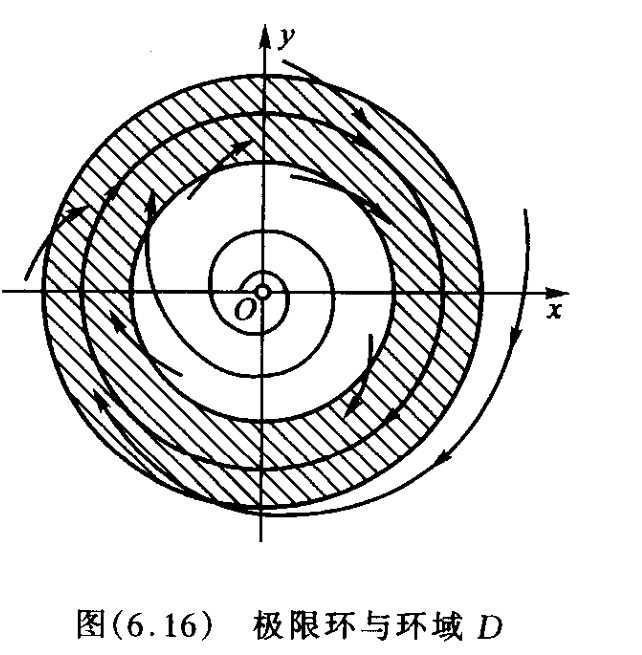
\includegraphics[width=\textwidth]{极限环.png}
    \caption{极限环}
    \label{fig:极限环}
\end{marginfigure}

假设平面驻定微分方程组
\begin{equation}\label{eq:6.33}
    \frac{\mathrm{d} x}{\mathrm{~d} t}=X(x, y), \quad \frac{\mathrm{d} y}{\mathrm{~d} t}=Y(x, y),
\end{equation}
其右端函数 $X, Y$ 在相平面的某域 $G$ 内有一阶连续偏导数。
\begin{theorem}
    如果 $G$ 内存在有界的环形闭域 $D$, 在其内不含有方程组 \eqref{eq:6.33} 的奇点,而 \eqref{eq:6.33} 的经过域 $D$ 上点的解 $x=x(t), y=$ $y(t)$ 当 $t \geqslant t_0$ (或 $t \leqslant t_0$ ) 时不离开该域, 则或者其本身是一个周期解(闭轨线),或者它按正向(或负向)趋近于 $D$ 内的某一周期解 (闭轨线).
\end{theorem}

\begin{theorem}[极限环的存在性]\label{theorem:limit_cycle_existence}
    如果于 $G$ 内存在单连通域 $D^*$, 在其内函数 $\frac{\partial X}{\partial x}+$ $\frac{\partial Y}{\partial y}$ 不变号且在 $D^*$ 内的任何子域上不恒等于零,则方程组 \eqref{eq:6.33} 在域 $D^*$ 内不存在任何周期解, 更不存在任何极限环.
\end{theorem}
\begin{proof}
    现在用反证法利用格林 (Green) 公式来证明定理. 假设 $D^*$ 内存在某周期为 $T$ 的周期解
    $$
        \Gamma: x=x(t), \quad y=y(t), \quad 0 \leqslant t \leqslant T,
    $$
    则对于由 $\Gamma$ 所围成的域 $D_{\Gamma}\left(\right.$ 显然 $\left.D_{\Gamma} \subset D^*\right)$ 有
    $$
        \begin{aligned}
              & \iint_{\mathrm{D}_{\Gamma}}\left(\frac{\partial X}{\partial x}+\frac{\partial Y}{\partial y}\right) \mathrm{d} x \mathrm{~d} y=\int_{\Gamma}(X \mathrm{~d} y-Y \mathrm{~d} x) \\
            = & \int_0^T\left(X \frac{\mathrm{~d} y}{\mathrm{~d} t}-Y \frac{\mathrm{~d} x}{\mathrm{~d} t}\right) \mathrm{d} t=\int_0^T(X Y-Y X) \mathrm{d} t=0,
        \end{aligned}
    $$
    这与定理的假设矛盾, 故在域 $D^*$ 内不存在任何周期解更不存在任何极限环。
\end{proof}

\section{奇点}

考虑二维(平面)一阶驻定微分方程组
\begin{equation}\label{eq:6.50}
    \begin{cases}
        \frac{\mathrm{d} x}{\mathrm{~d} t}=X(x, y), \\
        \frac{\mathrm{d} y}{\mathrm{~d} t}=Y(x, y),
    \end{cases}
\end{equation}
\begin{definition}[奇点]
    同时满足$X(x,y)=0$和$Y(x,y)=0$的点称为方程组的奇点。
\end{definition}
不妨设奇点为原点$(0,0)$,则$X(0,0)=Y(0,0)=0$。否则平移变换。

下面我们考虑驻定微分方程组是线性的情形下其轨线在相平面上的性态,并根据奇点邻域内轨线分布的不同性态来区分奇点的不同类型。这时方程的形式为
\begin{equation}\label{eq:6.51}
    \begin{cases}
        \frac{\mathrm{d} x}{\mathrm{~d} t}=a_{11}x+a_{12}y, \\
        \frac{\mathrm{d} y}{\mathrm{~d} t}=a_{21}x+a_{22}y,
    \end{cases}
\end{equation}
显然,坐标原点为奇点。如果方程组\ref{eq:6.51}的系数矩阵还满足
\[
    \begin{vmatrix}
        a_{11} & a_{12} \\
        a_{21} & a_{22}
    \end{vmatrix}\ne 0
\]
则此奇点还是唯一的。

根据线性代数的理论,我们知道,在线性变换下,奇点的类型是不变的,所以对于线性方程组\ref{eq:6.51},其奇点的类型与如下四种形式之一相同:
\[
    \left[\begin{array}{ll}\lambda & 0 \\ 0 & \mu\end{array}\right],\left[\begin{array}{ll}\lambda & 1 \\ 0 & \lambda\end{array}\right],\left[\begin{array}{ll}\lambda & 0 \\ 0 & \lambda\end{array}\right],\left[\begin{array}{rr}\alpha & \beta \\ -\beta & \alpha\end{array}\right]
\]
其中$\lambda,\mu,\alpha,\beta$为实数。这些标准形式是根据方程组\ref{eq:6.51}的特征方程来确定的。
\subsection{从特征根判断奇点类型}
\href{https://zhuanlan.zhihu.com/p/307458958}{见此文章总结}

奇点类型和特征根的关系如下:
\begin{table*}[ht!]
    \centering
    \begin{tabular}{ccc}
        \toprule
        奇点类型 & 特征根      & 稳定性条件            \\
        \midrule
        鞍点   & 实数异号     & 不稳定              \\
        结点   & 实数同号     & 实部为正时不稳定,实部为负时稳定 \\
        奇结点  & 重实数根     & 实部为正时不稳定,实部为负时稳定 \\
        焦点   & 复数,实部不为零 & 实部为正时不稳定,实部为负时稳定 \\
        中心   & 纯虚数      & 稳定,但不渐近稳定        \\
        \bottomrule
    \end{tabular}
    \caption{奇点类型、特征根与稳定性的关系}
    \label{tab:奇点类型与特征根的关系}
\end{table*}

\subsubsection{同号相异实根}
方程的标准类型为
$$\frac{\mathrm{d} \xi}{\mathrm{d} t}=\lambda_1 \xi, \frac{\mathrm{~d} \eta}{\mathrm{~d} t}=\lambda_2 \eta$$
相平面上的轨线形状如图\ref{fig:结点}所示。
\begin{figure}[h]
    \centering
    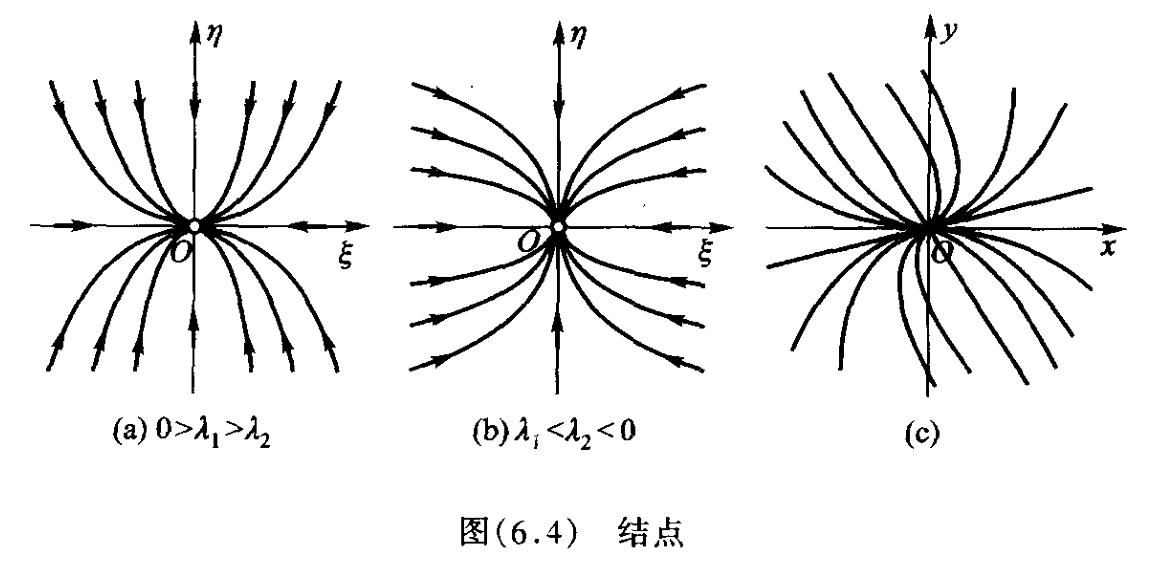
\includegraphics[width=\textwidth]{结点.png}
    \caption{结点}
    \label{fig:结点}
\end{figure}
图\ref{fig:结点}中,$\lambda_1,\lambda_2<0$,此时结点为\textbf{稳定结点},当$\lambda_1,\lambda_2>0$时,轨线走向相反。此时结点为\textbf{不稳定结点}。
\subsubsection{异号实根}

\begin{figure}[H]
    \centering
    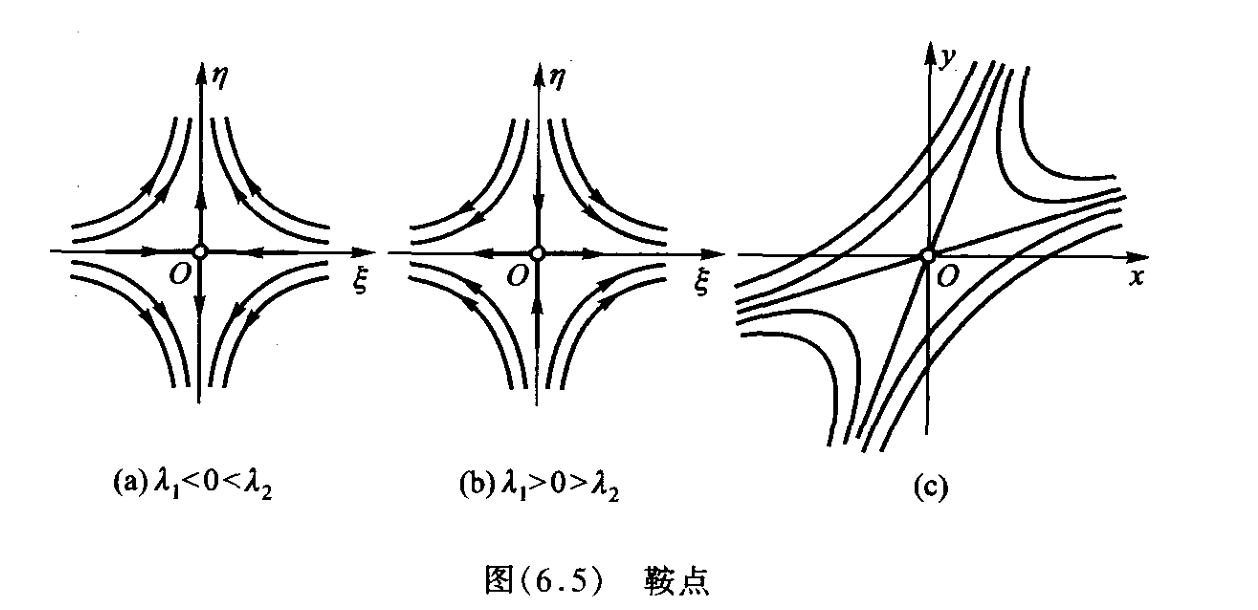
\includegraphics[width=\textwidth]{鞍点.png}
    \caption{鞍点}
    \label{fig:鞍点}
\end{figure}

\subsubsection{重根}
这时可以分两种情况讨论:

第一种是相似于
\[\left[\begin{array}{ll}\lambda & 1 \\ 0 & \lambda\end{array}\right]\]
方程可以化为
\[\frac{\mathrm{d} \xi}{\mathrm{d} t}=\lambda \xi+\eta, \quad \frac{\mathrm{d} \eta}{\mathrm{d} t}=\lambda \eta\]
其解为
\[
    \xi(t)=(At+B)\mathrm{e}^{\lambda t},\quad \eta(t)=A\mathrm{e}^{\lambda t}
\]
其中$\lambda$为实特征根,$A,B$为常数。
\begin{figure}[h]
    \centering
    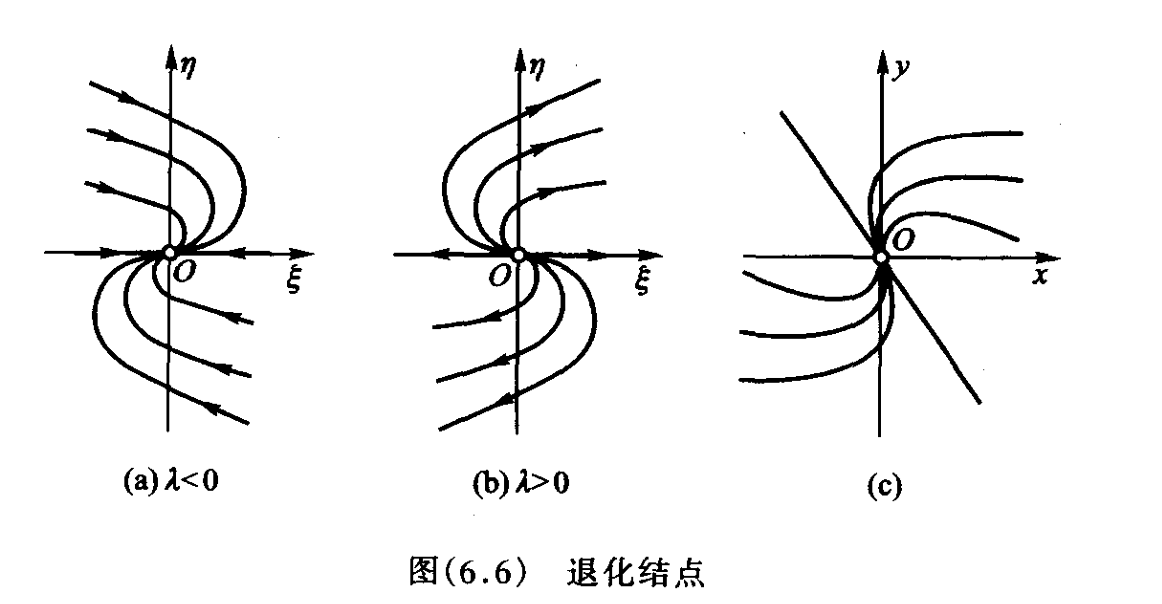
\includegraphics[width=\textwidth]{退化结点.png}
    \caption{退化结点}
    \label{fig:退化结点}
\end{figure}

第二种是相似于
\[\left[\begin{array}{ll}\lambda & 0 \\ 0 & \lambda\end{array}\right]\]
方程可以化为
\[\frac{\mathrm{d} x}{\mathrm{d} t}=\lambda x, \quad \frac{\mathrm{d} y}{\mathrm{d} t}=\lambda y\]
其解为
\[
    x(t)=A\mathrm{e}^{\lambda t},\quad y(t)=B\mathrm{e}^{\lambda t}
\]
其中$\lambda$为实特征根,$A,B$为常数。

于是
\[y=\frac{B}{A}x\]
\begin{figure}[h]
    \centering
    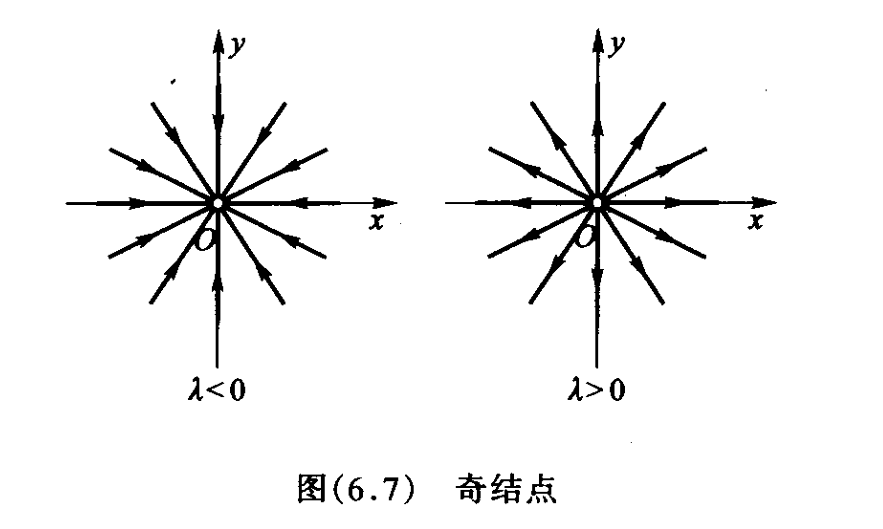
\includegraphics[width=\textwidth]{奇结点.png}
    \caption{奇结点}
    \label{fig:奇结点}
\end{figure}

\subsubsection{非零实部复根}
系数矩阵相似于
\[\left[\begin{array}{rr}\alpha & \beta \\ -\beta & \alpha\end{array}\right]\]
方程可以化为
\[\frac{\mathrm{d} \xi}{\mathrm{d} t}=\alpha \xi-\beta \eta, \quad \frac{\mathrm{d} \eta}{\mathrm{d} t}=\beta \xi+\alpha \eta\]
其解为
\[
    \xi(t)=A\mathrm{e}^{\alpha t}\cos(\beta t+\theta), \quad \eta(t)=A\mathrm{e}^{\alpha t}\sin(\beta t+\theta)
\]
其中$A,\theta$为常数。
\begin{figure}[h]
    \centering
    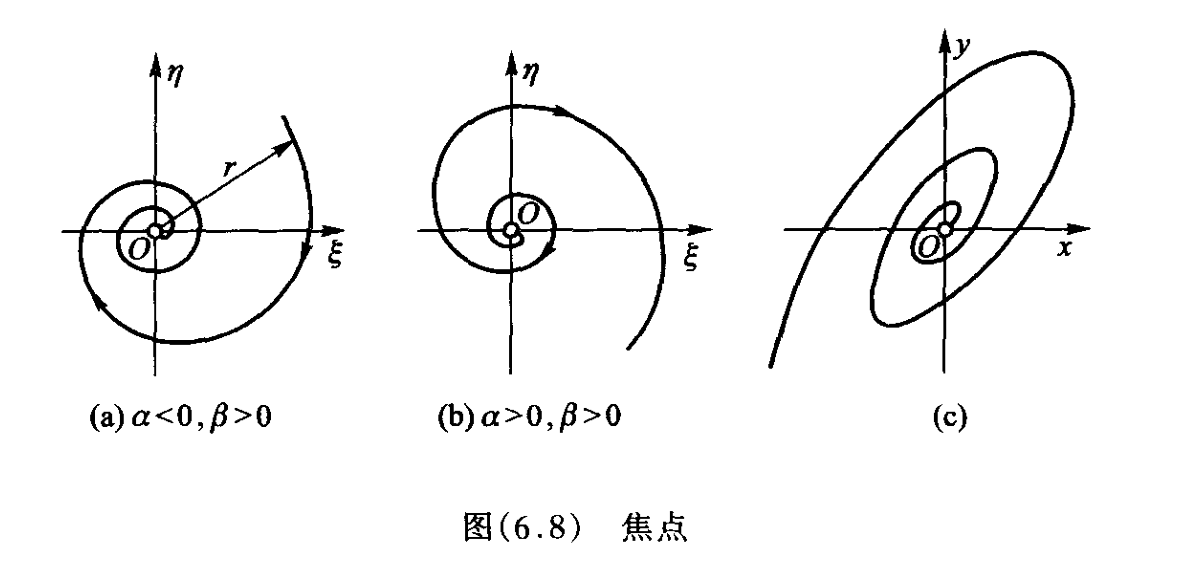
\includegraphics[width=\textwidth]{焦点.png}
    \caption{焦点}
    \label{fig:焦点}
\end{figure}

\subsubsection{纯虚根}
系数矩阵相似于\sidenote{也就是$\alpha=0$}
\[\left[\begin{array}{rr}0 & \beta \\ -\beta & 0\end{array}\right]\]
方程可以化为
\[\frac{\mathrm{d} x}{\mathrm{d} t}=-\beta y, \quad \frac{\mathrm{d} y}{\mathrm{d} t}=\beta x\]
其解为
\[
    x(t)=A\cos(\beta t+\theta), \quad y(t)=A\sin(\beta t+\theta)
\]
其中$A,\theta$为常数。
\begin{figure}[h]
    \centering
    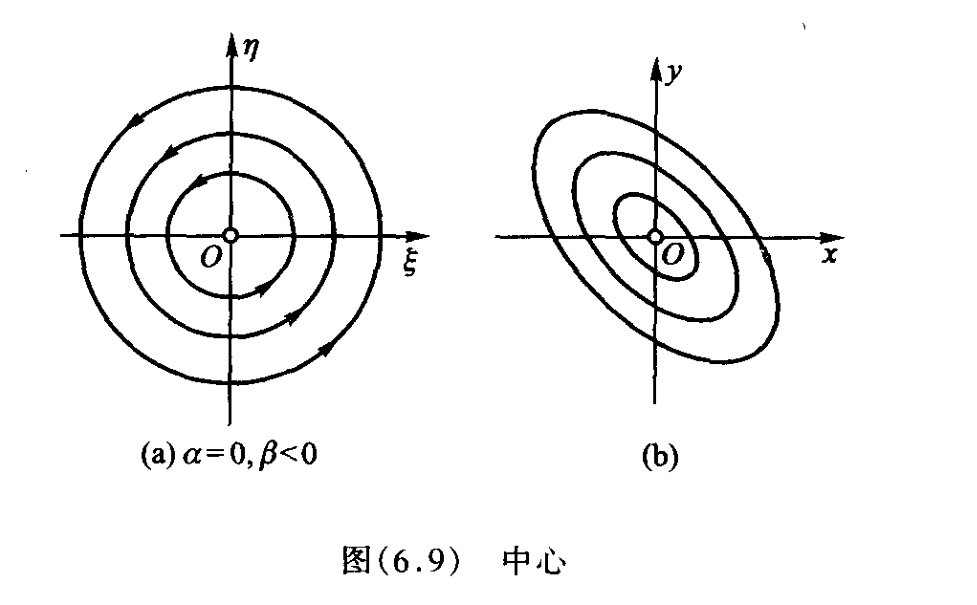
\includegraphics[width=\textwidth]{中心.png}
    \caption{中心}
    \label{fig:中心}
\end{figure}

\subsection{直接从特征方程判断奇点类型}
奇点的类型和特征方程的根之间的关系可以用图\ref{fig:奇点类型}来表示,对于特征方程
\[
    \lambda^2+p\lambda+q=0
\]
\begin{figure}[h]
    \centering
    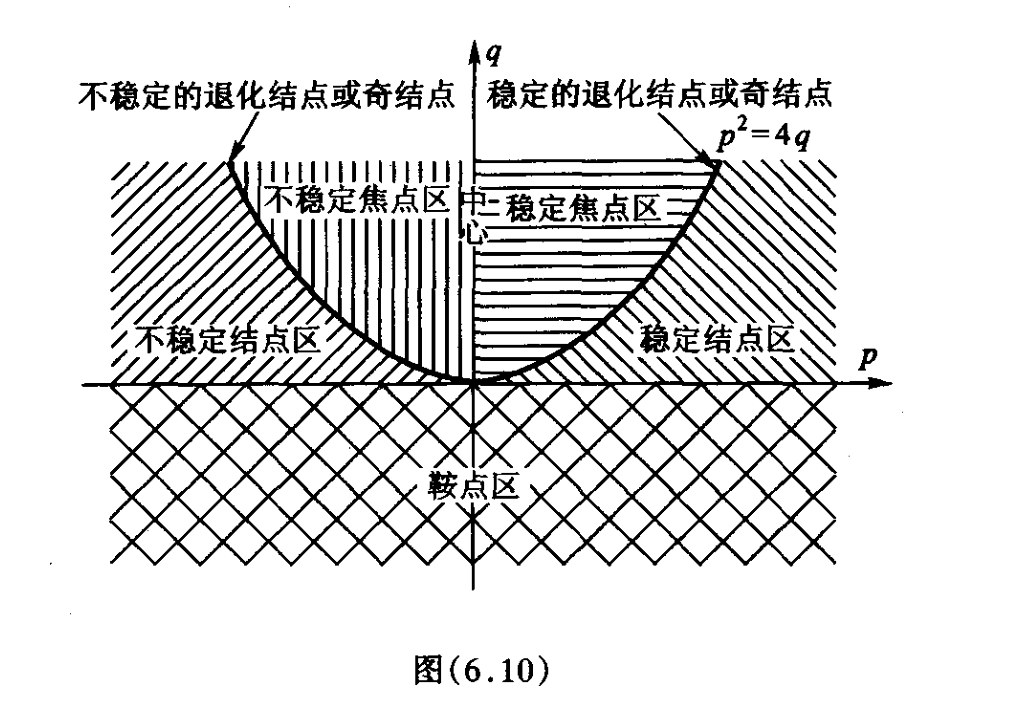
\includegraphics[width=\textwidth]{奇点类型.png}
    \caption{奇点类型}
    \label{fig:奇点类型}
\end{figure}

\section{练习}

\begin{exercise}
    $y^2(a d x-d y)-x(x+a y) d y=0$, 其中参数 $\mathrm{a}>0$;\marginnote{使用注意力}
\end{exercise}
\begin{remark}
    原方程可以变为齐次方程形式:$\frac{dy}{dx}=\frac{ay^2}{x^2+y^2+axy}$,但计算过程比较复杂。
\end{remark}
\begin{solution}
    注意到 $y\equiv 0$ 是特解: 若 $y\ne 0$ ,则原方程可变为: $\frac{y d x-x d y}{x^2+y^2}-\frac{1}{a y} d y=0$,因此通解为: $\arctan \frac{y}{x}-\frac{1}{a} \ln |y|=c$ 或 $y=x \tan \left(c+\frac{\ln |y|}{a}\right)$ ,其中, $c$ 是任意常数.
\end{solution}

\begin{exercise}
    $\frac{d}{d t}\binom{x}{y}=\left(\begin{array}{cc}-1 & 1 \\ 2 & 1\end{array}\right)\binom{x}{y}+\binom{e^{-t}}{0}$\marginnote{求解高阶微分方程,但是不使用特征根法}
\end{exercise}
\begin{remark}
    若用特征方法求解,容易出现计算错误。
\end{remark}
\begin{solution}
    由 $\left\{\begin{array}{c}x^{\prime}=-x+y+e^{-t} \\ y^{\prime}=2 x+y\end{array}\right.$ 得: $\left\{\begin{array}{l}y=x^{\prime}+x-e^{-t} \\ x^{\prime \prime}-3 x=-2 e^{-t}\end{array}\right.$

    现在求解方程: $\mathrm{x}^{\prime \prime}-3 \mathrm{x}=-2 e^{-t}$ 的通解为: $\mathrm{x}=c_1 e^{\sqrt{3} t}+c_2 e^{-\sqrt{3} t}+e^{-t}$

    最后, 原方程组的通解为:
    $\left\{\begin{array}{c}x=c_1 e^{\sqrt{3} t}+c_2 e^{-\sqrt{3} t}+e^{-t} \\ y=(1+\sqrt{3}) c_1 e^{\sqrt{3} t}+(1-\sqrt{3}) c_2 e^{-\sqrt{3} t}-e^{-t}\end{array}\right.$ ,其中 $c_1, c_2$ 为任意常数.
\end{solution}

\begin{exercise}
    对于一阶微分方程 $\frac{d y}{d x}=x^2-2 x y+y^2$,\marginnote{解的存在唯一性定理,Picard逐步逼近法,延拓解的存在区间,解对参数的偏导数}
    \begin{enumerate}
        \item 若 $-1 \leq x \leq 1,-1 \leq y \leq 1$, 试根据解的存在唯一性定理给出满足初始条件 $y(0)=0$ 的特解的存在区间;
        \item 若 $-1 \leq x \leq 1,-1 \leq y \leq 1$, 试根据Picard逐步逼近法给出满足初始条件 $y(0)=0$ 的二次近似解;
        \item 若 $-\infty \leq x \leq+\infty,-\infty \leq y \leq+\infty$, 试求满足初始条件 $y(0)=2$ 的延拓解的存在区间;
        \item 若 $-\infty \leq x \leq+\infty,-\infty \leq y \leq+\infty$ ,并记满足初始条件 $y\left(x_0\right)=y_0$ 的特解为 $\varphi\left(\mathrm{x} ; \mathrm{x}_0, \mathrm{y}_0\right)$, 试求偏导数函数: $\left.\frac{\partial \varphi\left(x ; x_0, y_0\right)}{\partial x_0}\right|_{x_0=0, y_0=1},\left.\frac{\partial \varphi\left(x ; x_0, y_0\right)}{\partial y_0}\right|_{x_0=0, y_0=1}$, $\left.\frac{\partial \varphi\left(x ; x_0, y_0\right)}{\partial x_0}\right|_{x_0=0, y_0=2},\left.\frac{\partial \varphi\left(x ; x_0, y_0\right)}{\partial y_0}\right|_{x_0=0, y_0=2}$ 的分析表达式.
    \end{enumerate}
\end{exercise}
\begin{solution}
    \begin{enumerate}
        \item 解: $f(x, y)=y^2-2 x y+x^2=(y-x)^2, a=1, b=1, M=\max |f(x, y)|=4$, $\mathrm{h}=\min \left(a, \frac{b}{M}\right)=\frac{1}{4}$. 因此, 解的存在区间为: $-\frac{1}{4} \leq x \leq \frac{1}{4}$
        \item 解: $x_0=0, \varphi_0(x)=y_0=0, \varphi_n(x)=y_0+\int_{x_0}^x f\left(s, \varphi_{n-1}(s)\right) d s, n=1,2, \ldots$

              一次近似解: $\varphi_1(x)=0+\int_0^x f\left(s, \varphi_0(s)\right) d s=\int_0^x(0-s)^2 d s=\frac{1}{3} x^3$
              二次近似解: $\varphi_2(x)=0+\int_0^x f\left(s, \varphi_1(s)\right) d s$
              $$
                  =\int_0^x\left(\frac{1}{3} s^3-s\right)^2 d s=\frac{1}{63} x^7-\frac{2}{15} x^5+\frac{1}{3} x^3
              $$
        \item 解: 对于 $\frac{d y}{d x}=(y-x)^2$, 令 $\mathrm{z}=\mathrm{y}-\mathrm{x}$, 则 $\frac{d z}{d x}=z^2-1=(z-1)(z+1)$,其通解为: $\mathrm{z}=\frac{1+c e^{2 x}}{1-c e^{2 x}}$, 其中 c 是任意常数, 因此 $\mathrm{y}=\mathrm{z}+\mathrm{x}=\frac{1+c e^{2 x}}{1-c e^{2 x}}+x$条件 $\mathrm{y}(0)=2$ 给出 $\mathrm{c}=\frac{1}{3}$, 因此满足 $\mathrm{y}(0)=2$ 的特解为: $\mathrm{y}=\frac{3+e^{2 x}}{3-e^{2 x}}+x$延拓解的存在区间为: $-\infty<x<\frac{1}{2} \ln 3$
    \end{enumerate}
\end{solution}

\begin{exercise}
    3. 设 $\boldsymbol{A}(t)$ 为区间 $a \leqslant t \leqslant b$ 上的连续 $n \times n$ 实矩阵, $\boldsymbol{\Phi}(t)$ 为方程 $\boldsymbol{x}'=$ $\boldsymbol{A}(t) \boldsymbol{x}$ 的基解矩阵,而 $\boldsymbol{x}=\boldsymbol{\varphi}(t)$ 为其一解。试证:
    \begin{enumerate}
        \item 对于方程 $\boldsymbol{y}'=-\boldsymbol{A}^{\mathrm{T}}(t) \boldsymbol{y}$ 的任一解 $\boldsymbol{y}=\boldsymbol{\psi}(t)$ 必有 $\boldsymbol{\psi}^{\mathrm{T}}(t) \boldsymbol{\varphi}(t)=$ 常数;
        \item $\boldsymbol{\Psi}(t)$ 为方程 $\boldsymbol{y}'=-\boldsymbol{A}^{\mathrm{T}}(t) \boldsymbol{y}$ 的基解矩阵的充要条件是存在非奇异的常数矩阵 $\boldsymbol{C}$, 使 $\boldsymbol{\Psi}^{\mathrm{T}}(t) \boldsymbol{\Phi}(t)=\boldsymbol{C}$.
    \end{enumerate}
\end{exercise}

\begin{proof}
    \begin{enumerate}
        \item 对于方程$\boldsymbol{y}'=-\boldsymbol{A}^{\mathrm{T}}(t) \boldsymbol{y}$,有$(y^\top)'=(y')^\top=(-A^\top y)^\top=-y^\top A$. 于是
              \[
                  \frac{d}{dt}(\boldsymbol{\psi}^\top \boldsymbol{\varphi})=(\boldsymbol{\psi}^\top)' \boldsymbol{\varphi}+\boldsymbol{\psi}^\top \boldsymbol{\varphi}'=-\boldsymbol{\psi}^\top A \boldsymbol{\varphi}+\boldsymbol{\psi}^\top A \boldsymbol{\varphi}=0
              \]
              于是$\boldsymbol{\psi}^\top \boldsymbol{\varphi}$为常数.
        \item 显然.
    \end{enumerate}
\end{proof}

\begin{exercise}
    $Y$是$\boldsymbol{x}'=\boldsymbol{A}(t)\boldsymbol{x}$的基解矩阵当且仅当$(Y^{-1})^{\top}$是$\boldsymbol{y}'=-\boldsymbol{A}^{\top}(t)\boldsymbol{y}$的一个基解矩阵.\sidenote{矩阵函数
        \[Q(t)=\begin{bmatrix}
                q_{11}(t) & q_{12}(t) & \cdots & q_{1n}(t) \\
                q_{21}(t) & q_{22}(t) & \cdots & q_{2n}(t) \\
                \vdots    & \vdots    & \ddots & \vdots    \\
                q_{n1}(t) & q_{n2}(t) & \cdots & q_{nn}(t)
            \end{bmatrix}
        \]
        被称为可微的,如果它的每个元素$q_{ij}(t)$都可微. 且$Q'(t)$被定义为
        \[
            Q'(t)=\begin{bmatrix}
                q_{11}'(t) & q_{12}'(t) & \cdots & q_{1n}'(t) \\
                q_{21}'(t) & q_{22}'(t) & \cdots & q_{2n}'(t) \\
                \vdots     & \vdots     & \ddots & \vdots     \\
                q_{n1}'(t) & q_{n2}'(t) & \cdots & q_{nn}'(t)
            \end{bmatrix}
        \]
    }
\end{exercise}

\begin{proof}
    对$Y^{-1}Y=I$两边求导,得到
    \[
        (Y^{-1}Y)'=Y^{-1}Y'+(Y^{-1})'Y=0
    \]
    于是$(Y^{-1}) ' Y=-Y^{-1}Y'=-Y^{-1}A(t)$. 由于$Y'=A(t)Y$,所以
    \[
        (Y^{-1})'=-Y^{-1}A(t)Y^{-1}=-Y^{-1}A(t)
    \]
    于是$((Y^{-1})^{\top})'=-A^{\top}(t)(Y^{-1})^{\top}$.
\end{proof}

\begin{exercise}
    求解 $x^{\prime \prime}(t)-9 x(t)=\mathrm{e}^{-3 t}\left(t^2+\sin 3 t\right)$.
\end{exercise}
\begin{solution}
    假设 $x(t)=\left(a t^3+b t^2+c t+m \cos 3 t+n \sin 3 t\right) \mathrm{e}^{-3 t}$, 则
    \[
        \frac{-18 a t^2+6 a t-12 b t+2 b-6 c+(18 m-9 n) \sin 3 t-(9 m+18 n) \cos 3 t}{\mathrm{e}^{3 t}}=\frac{t^2+\sin 3 t}{\mathrm{e}^{3 t}}
    \]
    解方程,得 $x_{\mathrm{p}}(t)=\frac{-180 t^3-90 t^2-30 t-72 \sin (3 t)+144 \cos (3 t)-5}{3240 \mathrm{e}^{3 t}}$ 为一特解。显然对应齐次方程的通解为 $x_{\mathrm{g}}(t)=c_1 \mathrm{e}^{3 t}+c_2 \mathrm{e}^{-3 t}$, 故所有解是
    \[
        x(t)=\frac{-180 t^3-90 t^2-30 t-72 \sin (3 t)+144 \cos (3 t)-5}{3240 \mathrm{e}^{3 t}}+c_1 \mathrm{e}^{3 t}+c_2 \mathrm{e}^{-3 t}
    \]
\end{solution}

\begin{exercise}
    考虑微分方程组: $\left\{\begin{array}{l}x^{\prime}=-x+y-x y^2 \\ y^{\prime}=-x-y-x^2 y\end{array}\right.$\marginnote{李雅普诺夫函数,极限环的存在性}
    \begin{enumerate}
        \item 试通过构造李雅谱洛夫函数,证明原点是渐近稳定的。(5 分)
        \item 试证明该系统在整个平面上无极限环。(5 分)
    \end{enumerate}
\end{exercise}

\begin{solution}
    \begin{enumerate}
        \item 构造李雅普诺夫函数$V(x,y)=x^2+y^2$,则
              \[
                  \frac{dV}{dt}=\frac{\partial V}{\partial x}\frac{dx}{dt}+\frac{\partial V}{\partial y}\frac{dy}{dt}=-2x^2-2y^2-4x^2y^2<0\quad(x,y)\ne (0,0)
              \]
              因此原点是渐近稳定的。
        \item 利用定理\ref{theorem:limit_cycle_existence},只需证明$\frac{\partial X}{\partial x}+\frac{\partial Y}{\partial y}$在平面上不变号且在平面上不为零。
              \[
                  \frac{\partial X}{\partial x}+\frac{\partial Y}{\partial y}=-1-1-x^2-y^2<0
              \]
              因此该系统在整个平面上无极限环。
    \end{enumerate}
\end{solution}

\begin{exercise}
    五. (20 分) 求出下列平面系统的所有奇点, 并判断奇点在相应线性近似方程中的类型:\marginnote{求解奇点并判断类型}
    $$
        \left\{\begin{array}{l}
            \frac{d x}{d t}=x^2-4 y \\
            \frac{d y}{d t}=x^2-(y-3)^2
        \end{array}\right.
    $$
\end{exercise}

\begin{solution}
    $$
        \left\{\begin{aligned}
            x^2-4 y     & =0 \\
            x^2-(y-3)^2 & =0
        \end{aligned}\right.
    $$
    $\Rightarrow(2,1),(-2,1),(6,9),(-6,9)$ 为所有奇点.
    $\left(x_0, y_0\right)$ 处线性近似对应矩阵
    $$
        \begin{gathered}
            A\left(x_0, y_0\right)=\left.\left(\begin{array}{ll}
                    2 x & -4      \\
                    2 x & -2(y-3)
                \end{array}\right)\right|_{\left(x_0, y_0\right)} \\
            A(2,1)=\left(\begin{array}{ll}
                    4 & -4 \\
                    4 & 4
                \end{array}\right) \\
            \operatorname{det}(A(2,1)-\lambda I)=\lambda^2-8 \lambda+32=(\lambda-4-4 i)(\lambda-4+4 i)
        \end{gathered}
    $$
    特征值为具有正实部的复数, $(2,1)$ 为(不稳定)焦点。
    同理可以知道 $A(-2,1)$ 特征值为 $\pm 4 \sqrt{2}$ 异号实数, $(-2,1)$ 为鞍点; $A(6,9)$ 特征值为 $\pm 4 \sqrt{6}$ 异号实数, $(6,9)$ 为鞍点; $A(-6,9)$ 特征值为 $-12 \pm 4 \sqrt{3}$ 为同号相异实数且同为负数, $(-2,1)$ 为稳定结点.
\end{solution}

\begin{exercise}
    12.已知方程组
    $$
        \left\{\begin{array}{l}
            \frac{\mathrm{d} x_1}{\mathrm{~d} t}=\frac{1}{t} x_1-x_2+t, \\
            \frac{\mathrm{~d} x_2}{\mathrm{~d} t}=\frac{1}{t^2} x_1+\frac{2}{t} x_2-t^2,
        \end{array} \quad t>0\right.
    $$
    的对应齐次方程组有解 $x_1=t^2, x_2=-t$ ,求其通解.
\end{exercise}
\begin{solution}
    由定理\ref{thm:4.8},设对应的齐次方程有另一解$y_1,y_2$,则
    $$
        \begin{vmatrix}
            t^2 & y_1 \\
            -t & y_2
        \end{vmatrix}=\exp\left(\int\frac{1}{t}+\frac{2}{t}dt\right)=t^3
    $$
    也就是$y_1=t^2-ty_2$,带入齐次方程组的第2个方程得到$\frac{dy_2}{dt}=t^{-1}y_2+1$,解得$y_2=t\ln t$,从而$y_1=t^2-t^2\ln t$,于是有基解矩阵
    \[
        \Phi(t)=\begin{bmatrix}
            t^2 & t^2(1-\ln t) \\
            -t & t\ln t
        \end{bmatrix}
    \]
    现在利用常数变易法求解非线性方程组的一个特解,只需照章办事,就有
    $$
        \tilde{x}=\begin{bmatrix}
            \frac{t^2}{2}\ln t-\frac{t^2}{2}(\ln t)^2+\frac{t^4}{4}-\frac{t^2}{4} \\
            \frac{t}{2}(\ln t)^2+\frac{t}{2}\ln t -\frac{3}{4}t^3+\frac{3}{4}t
        \end{bmatrix}
    $$
    于是通解为
    \[
        x=t^2\begin{bmatrix}
            t^2 & t^2(1-\ln t) \\
            -t & t\ln t
        \end{bmatrix}\begin{bmatrix}c_1 \\ c_2\end{bmatrix}+\begin{bmatrix}
            \frac{t^2}{2}\ln t-\frac{t^2}{2}(\ln t)^2+\frac{t^4}{4}-\frac{t^2}{4} \\
            \frac{t}{2}(\ln t)^2+\frac{t}{2}\ln t -\frac{3}{4}t^3+\frac{3}{4}t
        \end{bmatrix}
    \]
\end{solution}



\begin{thebibliography}{99}
    \bibitem{王高雄} 王高雄, 周之铭, 朱思铭, 王寿松. 常微分方程[M]. 第三版. 高等教育出版社, 2006.
    \bibitem{张伟年} 张伟年, 杜正东, 徐冰. 常微分方程[M]. 第二版. 高等教育出版社, 2014.
    \bibitem{Trench} William F. Trench. Elementary Differential Equations. 2013.
    \bibitem{Arnold} V.I.Arnold. Ordinary Differential Equations. 2010.
    \bibitem{Walter} Wolfgang Walter. Ordinary Differential Equations. Graduate Texts in Mathematics, Vol. 182. Springer-Verlag, 1998.
\end{thebibliography}


\setchapterimage[8cm]{Paul Pastourmatzis Unsplash}
\setchapterpreamble[u]{\margintoc}
\chapter{概率论}
\labch{probability}

\section{集合理论}

概率论中的$\subset$可能表示包含关系,也可能表示真包含关系. 而$\subseteq$一定表示包含关系,$\subsetneq$一定表示真包含关系.

$\sigma$-代数又叫$\sigma$-域.

\begin{definition}[概率空间]
    设 $\Omega$ 为样本空间, $\mathscr{F}$ 为 $\Omega$ 的部分子集构成的 $\sigma$-代数. 如果存在定义在 $\mathscr{F}$ 上而取值于 $[0,1]$ 的函数 $P$ ,满足
    \begin{enumerate}[label=(\roman*)]
        \item 规范性: $P(\Omega)=1$;
        \item 可列可加性:对 $A_i \in \mathscr{F}, i=1,2, \cdots$ ,且 $A_i \cap A_j=\emptyset, i \neq j$ ,有
              $$
                  P\left(\bigcup_{i=1}^{\infty} A_i\right)=\sum_{i=1}^{\infty} P\left(A_i\right),
              $$
    \end{enumerate}
    则称 $\mathscr{F}$ 为事件域, $P$ 为概率, $P(A)$ 为事件 $A \in \mathscr{F}$ 的概率, 三元组 $(\Omega, \mathscr{F}, P)$ 为概率空间.
\end{definition}


\subsection{Dynkin 定理}

\begin{definition}[$\pi$-系统、$\sigma$-代数、$\lambda$-系统]
    设 $S$ 是一个非空集合, $\mathcal{P}(S):=\{A \subseteq S\}$ 是 $S$ 的幂集. 称集族 $\mathcal{A} \subseteq \mathcal{P}(S)$ 是一个 $S$ 上的
    \begin{enumerate}
        \item $\pi$-系统, 如果 $\mathcal{A}$ 对集合的有限交运算封闭, 即 $A, B \in \mathcal{A} \Longrightarrow A \cap B \in \mathcal{A}$.
        \item $\sigma$-代数, 如果
              \begin{enumerate}[label=(\roman*)]
                  \item $S \in \mathcal{A}$
                  \item $\mathcal{A}$ 对集合的补运算封闭,即 $A \in \mathcal{A} \Longrightarrow A^c \in \mathcal{A}$
                  \item $\mathcal{A}$ 对集合的可数交\sidenote{可以等价替换为可数并,因为$\sigma$-代数对补运算封闭}运算封闭,即对可数多个\sidenote[][*2]{这里的可数多个如果替换为有限个,那它就成了代数的定义. $\sigma$通常表示可数多个}集合 $A_1, A_2, \cdots \in \mathcal{A}$ ,我们有
                        $$
                            \bigcap_{i=1}^{\infty} A_i \in \mathcal{A} .
                        $$
              \end{enumerate}
        \item $\lambda$-系统, 如果\footnote{如果满足前两条,则称为$\lambda_0$类,我们有$\pi$类+$\lambda_0$类=代数,而条件三等价于单调类,于是$\pi$类+$\lambda_0$类+单调类=$\sigma$代数}
              \begin{enumerate}[label=(\roman*)]
                  \item \label{def:lambda_system_1}$S \in \mathcal{A}$\marginnote{$\lambda$-系统定义中的\ref{def:lambda_system_1},\ref{def:lambda_system_2}说明$\lambda$-系统对集合的补运算封闭}
                  \item \label{def:lambda_system_2}$A, B \in \mathcal{A}, A \subseteq B \Longrightarrow B \backslash A \in \mathcal{A}$
                  \item \sidenote{可以等价替换为:设$A_1\subseteq A_2\subseteq \cdots$是$\mathcal{A}$中的可数多项的升链,则$$\bigcup_{i=1}^{\infty} A_i \in \mathcal{A}$$}设 $A_1, A_2, \cdots \in \mathcal{A}$ 是可数多个互不相交的集合, 则有
                        $$
                            \bigsqcup_{i=1}^{\infty} A_i \in \mathcal{A}
                        $$
              \end{enumerate}
    \end{enumerate}
\end{definition}

\begin{theorem}[Dynkin $\pi$-$\lambda$ 定理]\label{thm:dynkin_pi_lambda_theorem}
    设$\mathcal{F}\subseteq \mathcal{P}(S)$是一个$\pi$-系统,则
    $$
        \sigma(\mathcal{F})=\lambda(\mathcal{F})
    $$
\end{theorem}

\begin{theorem}[单调类定理]\label{thm:monotone_class_theorem}
    设$\mathcal{F}\subseteq \mathcal{P}(S)$是一个代数,则
    $$
        \sigma(\mathcal{F})=M(\mathcal{F})
    $$
\end{theorem}

\begin{theorem}
    单调类定理\ref{thm:monotone_class_theorem} 与 Dynkin 定理\ref{thm:dynkin_pi_lambda_theorem} 是等价的.
\end{theorem}

接下来我们总结一下这些集合系统之间的关系:
\begin{itemize}
    \item 所有的 $\sigma$-代数 $\subseteq$ 所有的 $\lambda$-系统 $\subseteq$ 所有的单调类
    \item 所有的 $\sigma$-代数 $\subseteq$ 所有的代数 $\subseteq$ 所有的 $\pi$-系统
    \item $\sigma$-代数 $=$ 单调类 + 代数 $=$ $\lambda$-系统 + $\pi$-系统
\end{itemize}

\section{离散型与连续型随机变量}

\begin{definition}[离散型随机变量]
    如果随机变量$X$ 的取值为有限个或可数个,则称$X$为离散型随机变量.
\end{definition}

以下就$X$取可数个值的情况进行讨论. 有限值情况类似.

设$X$是离散型随机变量,取值为$x_1,x_2,\cdots,x_n,\cdots$,则$X$的分布列定义为
$$
    p_k=\mathbb{P}(X=x_k)
$$
设函数$f(x)$取值于$\{x_1,x_2,\cdots\}$,$f(x_k)=p_k$,则称$f(x)$为随机变量$X$的概率质量函数(PMF, Probability Mass Function).

当分布列 $\left\{p_k\right\}$ 的规律性不够明显时, 也常常用如下的方式表达概率分布,
\begin{tabular}{c|cccc}
    $X$       & $x_1$ & $x_2$ & $x_3$ & $\cdots$ \\
    \hline$P$ & $p_1$ & $p_2$ & $p_3$ & $\cdots$
\end{tabular}
分布列具有如下性质:
\begin{itemize}
    \item $p_k\ge 0$
    \item $\sum_{k=1}^{\infty} p_k=1$\sidenote{因为对于$k\ne j$,$\{X=x_j\}$发生,$\{X=x_k\}$就不能发生,所以$\{X=x_j\},j=1,2,\cdots$是互不相容事件. 利用
              \[
                  \Omega=\bigcup_{k=1}^{\infty} \{X=x_k\}
              \]
              和概率的可列可加性得到
              \[
                  1=\mathbb{P}(\Omega)=\sum_{k=1}^{\infty} \mathbb{P}(X=x_k)=\sum_{k=1}^{\infty} p_k
              \]
          }
\end{itemize}


\begin{definition}[连续型随机变量]
    设$X$是随机变量,如果存在非负函数$f(x)$使得对任何满足$-\infty\le a<b\le \infty$的$a,b$,有
    $$
        \mathbb{P}(a\le X\le b)=\int_a^b f(x) \, dx
    $$
    则称$X$为连续型随机变量. 称$f(x)$为$X$的概率密度函数.
\end{definition}

设$f(x)$是$X$的概率密度,则$f(x)$有如下的基本性质.
\begin{itemize}
    \item $\int_{-\infty}^{\infty} f(x) \, dx=1$
    \item 对任意$a\in\mathbb{R}$,有$\mathbb{P}(X=a)=0$,于是
          $$
              \mathbb{P}(a\le X\le b)=\mathbb{P}(a<X\le b)=\mathbb{P}(a\le X<b)=\mathbb{P}(a<X<b)
          $$
    \item 对数集$A\in\mathcal{R}$,有
          $$
              \mathbb{P}(X\in A)=\int_A f(x) \, dx
          $$
\end{itemize}

\section{独立性}

\begin{definition}[独立性]
    \begin{itemize}
        \item 两个事件$A,B$独立\footnote{若$A,B$独立,则$A^c,B$独立,$A,B^c$独立,$A^c,B^c$独立. 证明思路是将$A\cup B$看成全集再 Subtract.},当且仅当$\mathbb{P}(A\cap B)=\mathbb{P}(A)\mathbb{P}(B)$.\marginnote{事件$A,B$独立,当且仅当随机变量$\mathbb{1}_A,\mathbb{1}_B$独立}
        \item 两个随机变量$X,Y$独立\footnote{若$X,Y$独立,则$\sigma(X),\sigma(Y)$独立.},当且仅当对任意$C,D\in\mathcal{R}$,有$\mathbb{P}(X\in C, Y\in D)=\mathbb{P}(X\in C)\mathbb{P}(Y\in D)$.\sidenote{也就是说,事件$A=\{X\in C\}$与$B=\{Y\in D\}$独立}
        \item 两个$\sigma$-域$\mathcal{F},\mathcal{G}$独立,当且仅当对任意$A\in\mathcal{F}$,$B\in\mathcal{G}$,有$\mathbb{P}(A\cap B)=\mathbb{P}(A)\mathbb{P}(B)$.
    \end{itemize}
\end{definition}

\begin{kaobox}[frametitle="独立"与"两两独立"]
    对于事件$A_1,A_2,\cdots,A_n$,
    \begin{itemize}
        \item 独立\sidenote[][*-4]{即对于任意指标$I\subset \{1,2,\cdots,n\}$,有$\mathbb{P}\left(\bigcap_{i\in I}A_i\right)=\prod_{i\in I}\mathbb{P}(A_i)$}一定两两独立\sidenote[][*-1]{即$\mathbb{P}(A_i\cap A_j)=\mathbb{P}(A_i)\mathbb{P}(A_j)$对任意$i\ne j$成立}
        \item 两两独立不一定独立\sidenote[]{反例考虑:设$X_1,X_2,X_3$是独立的随机变量,且$\mathbb{P}(X_i=0)=\mathbb{P}(X_i=1)=1/2$. 令$A_1=\{X_2=X_3\}$,$A_2=\{X_3=X_1\}$,$A_3=\{X_1=X_2\}$. 这些事件两两独立但不独立,因为$\mathbb{P}(A_1\cap A_2\cap A_3)=1/4\ne 1/8=\mathbb{P}(A_1)\mathbb{P}(A_2)\mathbb{P}(A_3)$}
    \end{itemize}
\end{kaobox}

\begin{definition}[集合类的独立]\label{def:集合类的独立}
    集合类$A_1,A_2,\cdots,A_n\in\mathcal{F}$被称为独立,如果对任意$A_i\in\mathcal{A}_i$和$I\subset \{1,2,\cdots,n\}$,有$\mathbb{P}(\bigcap_{i\in I}A_i)=\prod_{i\in I}\mathbb{P}(A_i)$.
\end{definition}

\begin{lemma}
    不失一般性,可以假设每个$\mathcal{A}_i$都包含全集$\Omega$. 那么定义\ref{def:集合类的独立}中等价于
    $$
        \mathbb{P}\left(\bigcap_{i\in I}A_i\right)=\prod_{i\in I}\mathbb{P}(A_i)\qquad \text{whenever } A_i\in\mathcal{A}_i\sidenote{因为对于$i\notin I$,可以令$A_i=\Omega$,这样就不用定义$I$了.}
    $$
\end{lemma}

\begin{theorem}\label{thm:independence_of_sigma_algebras}
    假设集合类$\mathcal{A}_1,\mathcal{A}_2,\cdots,\mathcal{A}_n$独立,且$\mathcal{A}_i$是$\pi$-系统,那么$\sigma(\mathcal{A}_1),\sigma(\mathcal{A}_2),\cdots,\sigma(\mathcal{A}_n)$也独立.
\end{theorem}

在数学中,想要证明某个性质对一个很大的集合成立,只需要证明这个性质对于集合的生成元成立即可. 如下的定理就利用了这个思想,目标是对于实数上的Borel代数成立,但是只需要对形如$\{(-\infty,a):a\in \mathbb{R}\}$的集合成立即可.\sidenote{甚至只需对$\{(-\infty,a):a\in \mathbb{Q}\}$证明成立即可. 因为一列可数个有理数可以逼近任意实数.}因为$\sigma(\{(-\infty,a):a\in \mathbb{R}\})=\mathcal{B}$.

\begin{theorem}
    为了证明$X_1,X_2,\cdots,X_n$独立,只需要证明:对于任意$x_1,x_2,\cdots,x_n\in (-\infty,\infty]$,有
    $$
        \mathbb{P}\left(\bigcap_{i=1}^n \{X_i\le x_i\}\right)=\prod_{i=1}^n \mathbb{P}(X_i\le x_i)
    $$
\end{theorem}

\begin{proof}
    令$\mathcal{A}_i$为形如$\{X_i\le x_i\}$的集合类,这显然是$\pi$-系统,由下面的练习\ref{ex:sigma_algebra_generated_by_inverse_image}可知,$\sigma(\mathcal{A}_i)=\sigma(X_i)$,所以根据定理\ref{thm:independence_of_sigma_algebras}就得到结果.
\end{proof}

\begin{exercise}\label{ex:sigma_algebra_generated_by_inverse_image}
    证明:若$\mathcal{A}$生成$\mathcal{S}$,那么$X^{-1}\coloneqq \{\{X\in A\}:A\in\mathcal{A}\}$生成$\sigma(X)=\{\{X\in B\}:B\in\mathcal{S}\}$.
\end{exercise}

\begin{proof}
    照章办事. 令$\mathcal{G}$是包含$X^{-1}(\mathcal{A})$的最小$\sigma$-代数. 因为$\sigma(X)$是包含$X^{-1}(\mathcal{A})$的$\sigma$-代数,所以$\sigma(X)\subseteq \mathcal{G}$. 职是之故,存在$\sigma$-域\sidenote{因为$\mathcal{G}$是$\sigma$-域.}$\mathcal{F}$满足$\mathcal{A}\subset \mathcal{F}\subset\mathcal{S}$,使得有$\mathcal{G}=\{\{X\in B\}:B\in\mathcal{S}\}$. 由于$\mathcal{S}$是由$\mathcal{A}$生成的,所以$\mathcal{F}=\mathcal{S}$.
\end{proof}

\begin{theorem}\label{thm:independence_of_sigma_algebras_2}
    令集合类\marginnote{这是二维的情况}$\mathcal{F}_{i,j},1\le i\le n,1\le j\le m(i)$独立,令$\mathcal{G}_i=\sigma(\cup_{j=1}^{m(i)}\mathcal{F}_{i,j})$. 则$\mathcal{G}_1,\mathcal{G}_2,\cdots,\mathcal{G}_n$独立.
\end{theorem}

\begin{proof}
    令$\mathcal{A}_i$为具有形式$\cap_j A_{i,j}$的集合类(其中$A_{i,j}\in\mathcal{F}_{i,j}$),显然$\mathcal{A}_i$是$\pi$-系统,包含$\Omega$和$\cup_j\mathcal{F}_{i,j}$,所以根据定理\ref{thm:independence_of_sigma_algebras}就得到:$\sigma(\mathcal{A}_i)=\mathcal{G}_i$独立.
\end{proof}

\begin{theorem}\label{thm:independence_of_inverse_image}
    若$X_{i,j},1\le i\le n,1\le j\le m(i)$独立,$f_i:\mathbf{R}^{m(i)}\to \mathbf{R}$可测,那么$f_i(X_{i,1},X_{i,2},\cdots,X_{i,m(i)})$独立.
\end{theorem}

\begin{proof}
    令$\mathcal{F}_{i,j}=\sigma(X_{i,j})$,则$\mathcal{F}_{i,j}$独立,令$\mathcal{G}_i=\sigma(\cup_j\mathcal{F}_{i,j})$,则根据定理\ref{thm:independence_of_sigma_algebras_2},$\mathcal{G}_1,\mathcal{G}_2,\cdots,\mathcal{G}_n$独立,........未完待续\sidenote{没有搞懂这个证明.}
\end{proof}

定理\ref{thm:independence_of_inverse_image}的特殊情况是:若$X_1,X_2,\cdots,X_n$独立,则$X_1$与$X_2\cdots X_n$独立. 而且,$X_1+X_2+\cdots+X_n$与$X_1,X_2,\cdots ,X_n$独立.

\begin{exercise}
    若$(X_1,X_2,\cdots,X_n)$有概率密度$f(x_1,x_2,\cdots,x_n)$\sidenote[][*1]{即对于任意$A\in\mathcal{R}^n$,有$$
    \begin{aligned}
        & \quad \mathbb{P}((X_1,X_2,\cdots,X_n)\in A) \\
        & = \int_A f(x_1,x_2,\cdots,x_n) \, dx
    \end{aligned}
    $$},且$f(x)$可以被写成$g(x_1)g(x_2)\cdots g(x_n)$,其中$g_m\ge 0$,则$X_1,X_2,\cdots,X_n$独立.\footnote{$g_m$并不必为概率密度函数.}
\end{exercise}

\begin{proposition}
    \begin{itemize}
        \item 设 $(\xi, \eta)$ 是离散型随机变量, 那么它们独立的充要条件是联合分布列等于两个边沿分布列的乘积.
        \item 设 $(\xi, \eta)$ 是连续型随机变量, 那么它们独立的充要条件是联合密度函数在其连续点上等于两个边沿密度函数的乘积.
    \end{itemize}
\end{proposition}

现在考虑下面的问题: 如果 $\xi, \eta$ 是随机变量, $f \in \mathscr{B}^2$. 问: 在求期望 $E[f(\xi, \eta)]$ 时, 能否先固定一个, 即先求 $E[f(x, \eta)]$, 得到 $x$ 的函数, 再将 $\xi$ 代入到这个函数中去, 得到一个随机变量,然后求这个随机变量的期望?\sidenote{回答一般是否定的. 例如,取 $f(x, y)=x y$ . 此时,对任意两个随机变量 $\xi, \eta$ ,上面公式成立意味着 $E[\xi \eta]=E[\xi] E[\eta]$ ,即 $\xi, \eta$ 不相关. 这显然一般是不对的. 比如, $\xi=\eta, \xi$ 是对称随机变量 $(\xi$ 与 $-\xi$ 同分布 $), E[\xi]=0$ (例如 $\xi \sim N(0,1))$. 则
$$
    \varphi(x):=E[x \eta]=0, \quad \forall x,
$$
于是
$$
    E[\varphi(\xi)]=0
$$
但显然
$$
    E[f(\xi, \eta)]=E\left[\xi^2\right] \neq 0
$$}

但是在独立的情形下, 这个结论是成立的. 我们有如下的定理:
\begin{theorem}\label{thm:independence_of_random_variables_and_expectation}
    设 $f: \mathbb{R}^2 \mapsto \mathbb{R}$ 为非负 Borel可测, $(\xi, \eta)$ 为二维随机变量. 令
    $$
        \varphi(x):=E[f(x, \eta)] .
    $$
    则 $\varphi: \mathbb{R} \mapsto \mathbb{R}$ 为非负 Borel可测,且 $\xi, \eta$ 为独立的充要条件对任意这样的 $f$,
    $$
        E[f(\xi, \eta)]=E[\varphi(\xi)] .
    $$
\end{theorem}
\begin{note}
    这个定理是条件期望的一个应用.
\end{note}
\begin{proof}
    先证$\varphi$的Borel可测性,由于非负可测函数可以由非负简单函数单调上升地逼近,所以由单调收敛定理,只需对$f$是非负简单函数证明. 而由期望的线性性,这又归结为对示性函数证明. 因此我们设
    \[f=1_A,\quad A\in\mathscr{B}^2\]
    令
    $$
        \mathscr{G}:=\left\{A \in \mathscr{B}^2: \varphi(x):=E\left[1_A(x, \eta)\right] \text { 为Borel可测 }\right\} .
    $$
    则易证 $\mathscr{G}$ 为 $\lambda$-类, 且包含了 $\pi$-类:
    $$
        \Pi:=\{(-\infty, a] \times(-\infty, b], a, b \in \mathbb{R}\} .
    $$
    因此由单调类定理有 $\mathscr{G}=\sigma(\Pi)=\mathscr{B}^2$.

    下面证第二个结论. 充分性显然,因为取
    $$
        f(x, y):=1_{(-\infty, a]}(x) \cdot 1_{(-\infty, b]}(y),
    $$
    则
    $$
        E[f(\xi, \eta)]=E[\varphi(\xi)]
    $$
    就变为
    $$
        P(\xi \leqslant a, \eta \leqslant b)=P(\xi \leqslant a) P(\eta \leqslant b) .
    $$
    往证必要性. 令
    $$
        \begin{gathered}
            \mathscr{G}:=\left\{A \in \mathscr{B}^2: \text { 定理对函数 } f:=1_A \text { 成立 }\right\} . \\
            \mathscr{C}:=\{(a, b] \times(c, d]: a<b, c<d\} .
        \end{gathered}
    $$
    则 $\mathscr{C}$ 为 $\pi$-类, 且 $\mathscr{B}^2=\sigma(\mathscr{C})$. 对 $A:=(a, b] \times(c, d] \in \mathscr{C}$, 令
    $$
        f:=1_A .
    $$
    则
    $$
        \varphi(x)=E\left[1_A(x, \eta)\right]=1_{(a, b]}(x) E\left[1_{(c, d]}(\eta)\right]=1_{(a, b]}(x) P(c<\eta \leqslant d) .
    $$
    所以
    $$
        E[\varphi(\xi)]=E\left[1_{(a, b]}(\xi)\right] P(c<\eta \leqslant d)=P(a<\xi \leqslant b) P(c<\eta \leqslant d) .
    $$
    而由独立性也有
    $$
        \begin{aligned}
            E[f(\xi, \eta)] & =E\left[1_{(a, b] \times(c, d]}(\xi, \eta)\right] \\
                            & =P(a<\xi \leqslant b, c<\eta \leqslant d)         \\
                            & =P(a<\xi \leqslant b) P(c<\eta \leqslant d) .
        \end{aligned}
    $$
    所以, $\mathscr{C} \subset \mathscr{G}$.

    往证 $\mathscr{G}$ 为 $\lambda$-类. 显然 $\mathbb{R}^2 \in \mathscr{G}$. 设 $A, B \in \mathscr{G}, A \subset B$. 对任意 $C \subset \mathscr{B}^2$, 令
    $$
        \varphi_C(x):=E\left[1_C(x, \eta)\right],
    $$
    则
    $$
        E\left[\varphi_B(\xi)\right]-E\left[\varphi_A(\xi)\right]=E\left[\varphi_{B \backslash A}(\xi)\right] .
    $$
    因此
    $$
        \begin{aligned}
            E\left[1_{B \backslash A}(\xi, \eta)\right] & =E\left[1_B(\xi, \eta)-1_A(\xi, \eta)\right]               \\
                                                        & =E\left[1_B(\xi, \eta)\right]-E\left[1_A(\xi, \eta)\right] \\
                                                        & =E\left[\varphi_B(\xi)\right]-E\left[\varphi_A(\xi)\right] \\
                                                        & =E\left[\varphi_{B \backslash A}(\xi)\right] .
        \end{aligned}
    $$
    所以 $B-A \in \mathscr{G}$. 再设 $A_n \in \mathscr{G}, A_n \uparrow A$. 则由单调收敛定理有
    $$
        \begin{aligned}
            E\left[1_A(\xi, \eta)\right] & =\lim _{n \rightarrow \infty} E\left[1_{A_n}(\xi, \eta)\right] \\
                                         & =\lim _{n \rightarrow \infty} E\left[\varphi_{A_n}(\xi)\right] \\
                                         & =E\left[\lim _{n \rightarrow \infty} \varphi_{A_n}(\xi)\right] \\
                                         & =E\left[\varphi_A(\xi)\right]
        \end{aligned}
    $$
    所以 $A \in \mathscr{G}$. 这样, 由 $\lambda-\pi$ 定理, $\mathscr{G}$ 为 $\sigma$-代数. 于是 $\mathscr{G}=\mathscr{B}^2$.

    现在, 若 $f$ 是简单函数:
    $$
        f:=\sum_{k=1}^n a_k 1_{A_k}, \quad a_k \in \mathbb{R}, A_k \in \mathscr{B}^2,
    $$
    则有
    $$
        \begin{aligned}
            E[f(\xi, \eta)] & =\sum_{k=1}^n a_k E\left[1_{A_k}(\xi, \eta)\right] \\
                            & =\sum_{k=1}^n a_k E\left[\varphi_{A_k}(\xi)\right] \\
                            & =E\left[\sum_{k=1}^n a_k \varphi_{A_k}(\xi)\right] \\
                            & =E[\varphi(\xi)]
        \end{aligned}
    $$
    最后, 设 $f \geqslant 0, f \in \mathscr{B}^2$. 于是, 存在简单函数 $f_n \uparrow f$. 以 $\varphi_n$ 表示 $f_n$ 对应的 $\varphi$, 则由单调收敛定理,有
    $$
        \begin{aligned}
            E[f(\xi, \eta)] & =\lim _{n \rightarrow \infty} E\left[f_n(\xi, \eta)\right] \\
                            & =\lim _{n \rightarrow \infty} E\left[\varphi_n(\xi)\right] \\
                            & =E[\varphi(\xi)]
        \end{aligned}
    $$
\end{proof}
在定理\ref{thm:independence_of_random_variables_and_expectation}中,用$f(x,y)\cdot \mathbb{1}_{f(x,y)\in A}$替换$f(x,y)$,则有
\begin{corollary}
    延续定理\ref{thm:independence_of_random_variables_and_expectation}中的符号,若 $\xi, \eta$ 独立,则
    \[
        \mathbb{P}(f(\xi,\eta)\in A)=\mathbb{E}[\varphi(\eta)]
    \]
    其中$\varphi(y)=\mathbb{P}(f(\xi,y)\in A)$
\end{corollary}

\section{不相关与独立}

对于随机变量$\xi,\eta$,若$\mathbb{E}[\xi\eta]=\mathbb{E}[\xi]\mathbb{E}[\eta]$,则称$\xi,\eta$不相关. 也就是说他们的协方差为0.

自然地,独立意味着不相关,但是不相关并不意味着独立. 因为不相关是个整体的概念\sidenote{求期望是整体概念},而独立是局部概念.

\begin{note}
    但在一个重要的特殊情形,不相关和独立是等价的. 这就是$(\xi,\eta)$服从二维正态分布的情形.
\end{note}

\begin{theorem}
    如果$(\xi,\eta)$服从二维正态分布,则$\xi,\eta$不相关当且仅当$\xi,\eta$独立.
\end{theorem}

\begin{theorem}
    设$\xi$和$\eta$均为只取两个不同值的随机变量,那么$\xi$与$\eta$独立的充要条件是它们不相关.
\end{theorem}

\begin{proof}
    只用证明不相关\sidenote{$E[\xi\eta]=E[\xi]E[\eta]$.}推出独立性,不妨设$\xi,\eta\in\{0,1\}$,直接解方程即可验证$P(\xi=i,\eta=j)=P(\xi=i)P(\eta=j),i,j\in\{0,1\}$.
    \[
        \begin{array}{c|c|c|c}
                & X=0                              & X=1 &     \\
            \hline
            Y=0 & \begin{array}{c} p_1 \end{array} & p_2 & a   \\
            \hline
            Y=1 & p_3                              & p_4 & 1-a \\
            \hline
                & b                                & 1-b &     \\
        \end{array}
    \]
    由不相关性,可以知道$E[XY]=E[X]E[Y]$,即$p_4=(1-a)(1-b)$. 显然可以求出$p_1,p_2,p_3$,从而验证独立性.
\end{proof}

\section{分布}

% \begin{definition}[分布函数、概率密度函数]\label{def:distribution_function_and_probability_density_function}

% \end{definition}
\subsection{特殊分布函数}

\begin{itemize}
    \item 均匀分布 $U(a,b)$: 分布函数与概率密度函数为
          $$f(x)=\begin{cases}
                  0,               & x<a       \\
                  \frac{x-a}{b-a}, & x\in[a,b] \\
                  1,               & x>b
              \end{cases} \qquad p(x)=\begin{cases}
                  \frac{1}{b-a}, & x\in[a,b] \\
                  0,             & \text{其他}
              \end{cases}$$
          特征函数为
          $$\varphi(t) = \frac{e^{itb} - e^{ita}}{it(b-a)}$$
    \item 指数分布 $Exp(\lambda)$: 分布函数与概率密度函数为
          $$f(x)=\begin{cases}
                  1-e^{-\lambda x}, & x\geq 0 \\
                  0,                & x<0
              \end{cases} \qquad p(x)=\begin{cases}
                  \lambda e^{-\lambda x}, & x\geq 0 \\
                  0,                      & x<0
              \end{cases}$$
          特征函数为
          $$\varphi(t) = \frac{\lambda}{\lambda - it}$$
    \item 正态分布 $N(\mu,\sigma^2)$: 分布函数与概率密度函数为
          \begin{gather*}
              f(x)=\frac{1}{\sqrt{2\pi}\sigma}\int_{-\infty}^x e^{-\frac{(t-\mu)^2}{2\sigma^2}}dt \\
              p(x)=\frac{1}{\sqrt{2\pi}\sigma}e^{-\frac{(x-\mu)^2}{2\sigma^2}}, \quad x\in\mathbb{R}
          \end{gather*}
          特征函数为
          $$\varphi(t) = e^{i\mu t - \frac{1}{2}\sigma^2 t^2}$$
    \item 二项分布 $B(n,p)$: 分布函数与概率质量函数为
          $$f(x)=\sum_{k\leq x}\binom{n}{k}p^k(1-p)^{n-k} \qquad P(X=k)=\binom{n}{k}p^k(1-p)^{n-k}, \quad k=0,1,\ldots,n$$
          特征函数为
          $$\varphi(t) = \left(q + pe^{it}\right)^n, \quad q = 1-p$$
    \item 泊松分布 $P(\lambda)$: 分布函数与概率质量函数为
          $$f(x)=\sum_{k\leq x}\frac{\lambda^k}{k!}e^{-\lambda} \qquad P(X=k)=\frac{\lambda^k}{k!}e^{-\lambda}, \quad k=0,1,2,\ldots$$
          特征函数为
          $$\varphi(t) = e^{\lambda(e^{it} - 1)}$$
    \item 几何分布 $G(p)$: 分布函数与概率质量函数为
          $$f(x)=1-(1-p)^{\lfloor x \rfloor} \qquad P(X=k)=p(1-p)^{k-1}, \quad k=1,2,\ldots$$
          特征函数为
          $$\varphi(t) = \frac{pe^{it}}{1 - (1-p)e^{it}}$$
    \item 超几何分布 $H(N,M,n)$: 分布函数与概率质量函数为
          $$f(x)=\sum_{k\leq x}\frac{\binom{M}{k}\binom{N-M}{n-k}}{\binom{N}{n}} \qquad P(X=k)=\frac{\binom{M}{k}\binom{N-M}{n-k}}{\binom{N}{n}}, \quad k=\max(0,n-N+M),\ldots,\min(n,M)$$
          特征函数较复杂,通常不以简单形式表示。
    \item 负二项分布 $NB(r,p)$: 分布函数与概率质量函数为
          $$f(x)=\sum_{k\leq x}\binom{k+r-1}{k}p^r(1-p)^k \qquad P(X=k)=\binom{k+r-1}{k}p^r(1-p)^k, \quad k=0,1,2,\ldots$$
          特征函数为
          $$\varphi(t) = \left(\frac{p}{1 - (1-p)e^{it}}\right)^r$$
\end{itemize}

\begin{theorem}[gamma 分布的性质]
    若$X\sim gamma(\alpha,\lambda),Y=gamma(\beta,\lambda)$,且$X,Y$独立,则$X+Y\sim gamma(\alpha+\beta,\lambda)$.\footnote{证明只需照章办事,}
\end{theorem}

\begin{theorem}[正态分布的性质]
    若$X\sim normal(\mu ,a ),Y\sim normal(\nu,b)$,且$X,Y$独立,则$X+Y\sim normal(\mu+\nu,a+b)$.\footnote{证明只需照章办事.}
\end{theorem}

目前我们接触到的分布的关系为
\begin{itemize}
    \item $n$ 个独立同分布 $B(1, p)$ 的 0-1 分布随机变量之和服从二项分布 $B(n, p)$
    \item 若 $X_1\sim B(n_1,p),X_2\sim B(n_2,p)$ 且独立,则 $X_1+X_2\sim B(n_1+n_2,p)$
    \item 若 $X_1\sim P(\lambda_1),X_2\sim P(\lambda_2)$ 且独立,则 $X_1+X_2\sim P(\lambda_1+\lambda_2)$
    \item $r$ 个独立同分布几何分布 $G(p)$ 的随机变量之和服从参数为 $r$ 和 $p$ 的 Pascal 分布
    \item 若 $X_i\sim N(\mu_i,\sigma_i^2),i=1,\cdots,n$ 且独立,则对任意实数 $a_1,\cdots,a_n$,有
          $$\sum_{i=1}^n a_iX_i\sim N\left(\sum_{i=1}^n a_i\mu_i,\sum_{i=1}^n a_i^2\sigma_i^2\right)$$
\end{itemize}

\subsection{联合分布与边缘分布}
对于随机向量 $(X, Y)$, 我们称
$$
    F(x, y)=P(X \leq x, Y \leq y)
$$
为 $(X, Y)$ 的联合概率分布函数, 简称为联合分布 (joint distribution).
$$
    \begin{gathered}
        F_X(x)=P(X \leq x, Y \leq \infty)=F(x, \infty) \\
        F_Y(y)=P(X \leq \infty, Y \leq y)=F(\infty, y)
    \end{gathered}
$$
我们称 $X$ 的分布函数 $F_X(x)$, $Y$ 的分布函数 $F_Y(x)$ 为 $(X, Y)$ 的边缘分布函数 (marginal distribution function).

\begin{theorem}
    设 $X, Y$ 分别有概率密度 $f_X(x), f_Y(y)$. 则 $X, Y$ 独立的充分必要条件是随机向量 $(X, Y)$ 有联合密度
    $$
        f(x, y)=f_X(x) f_Y(y) .
    $$
\end{theorem}

\subsection{二维正态分布}
特别地,设 $(\xi, \eta)$ 服从二维正态分布 $N(\mu, \Sigma)$ ,其中 $\mu=\left(\mu_1, \mu_2\right)$ ,
$$
    \Sigma=\left(\begin{array}{cc}
            \sigma_1^2             & \rho \sigma_1 \sigma_2 \\
            \rho \sigma_1 \sigma_2 & \sigma_2^2
        \end{array}\right)
$$
其中 $\sigma_1, \sigma_2>0, \rho \in(-1,1)$ .则 $(\xi, \eta)$ 的密度函数写成分量形式为
$$
    \begin{aligned}
        p(x, y)= & \frac{1}{2 \pi \sigma_1 \sigma_2 \sqrt{1-\rho^2}} \exp \left\{-\frac{1}{2\left(1-\rho^2\right)}\right.                                                                                       \\
                 & \left.\cdot\left[\frac{\left(x-\mu_1\right)^2}{\sigma_1^2}-\frac{2 \rho\left(x-\mu_1\right)\left(y-\mu_2\right)}{\sigma_1 \sigma_2}+\frac{\left(y-\mu_2\right)^2}{\sigma_2^2}\right]\right\}
    \end{aligned}
$$
此时,也记为 $(\xi, \eta) \sim N\left(\mu_1, \mu_2, \sigma_1^2, \sigma_2^2, \rho\right)$ .图\ref{fig:二维正态分布}是 $N(5,5,1,1,0.5)$ 的密度函数图像.
\begin{marginfigure}
    \centering
    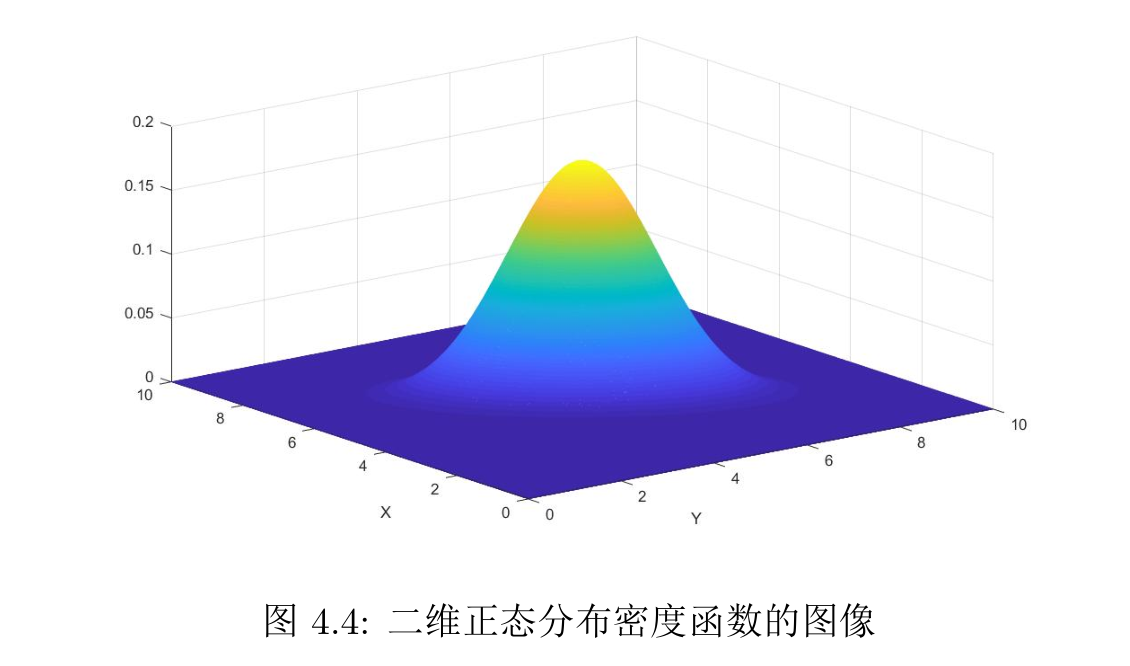
\includegraphics[width=\textwidth]{二维正态分布.png}
    \caption{二维正态分布的密度函数图像}
    \label{fig:二维正态分布}
\end{marginfigure}
现在求其边沿分布.为此将 $p(x, y)$ 改写为
$$
    \begin{aligned}
        p(x, y)= & \frac{1}{\sqrt{2 \pi} \sigma_1} \exp \left\{-\frac{\left(x-\mu_1\right)^2}{2 \sigma_1^2}\right\}                                                                                                                     \\
                 & \cdot \frac{1}{\sqrt{2 \pi\left(1-\rho^2\right)} \sigma_2} \exp \left\{-\frac{\left[y-\left(\mu_2+\rho \frac{\sigma_2}{\sigma_1}\left(x-\mu_1\right)\right]^2\right.}{2 \sigma_2^2\left(1-\rho^2\right)}\right\}     \\
        =        & \frac{1}{\sqrt{2 \pi} \sigma_2} \exp \left\{-\frac{\left(y-\mu_2\right)^2}{2 \sigma_2^2}\right\}                                                                                                                     \\
                 & \cdot \frac{1}{\sqrt{2 \pi\left(1-\rho^2\right)} \sigma_1} \exp \left\{-\frac{\left[x-\left(\mu_1+\rho_{\frac{\sigma_1}{\sigma_2}}\left(y-\mu_2\right)\right)\right]^2}{2 \sigma_1^2\left(1-\rho^2\right)}\right\} .
    \end{aligned}
$$
由此易得
$$
    \begin{aligned}
         & p_{\xi}(x)=\int_{\mathbb{R}} p(x, y) d y=\frac{1}{\sqrt{2 \pi} \sigma_1} e^{-\frac{\left(x-\mu_1\right)^2}{2 \sigma_1^2}}, \\
         & p_\eta(y)=\int_{\mathbb{R}} p(x, y) d x=\frac{1}{\sqrt{2 \pi} \sigma_2} e^{-\frac{\left(y-\mu_2\right)^2}{2 \sigma_2^2}} .
    \end{aligned}
$$
这就是说,正态分布的边沿分布仍为正态分布,$\xi \sim N\left(\mu_1, \sigma_1^2\right)$ 和 $\eta \sim N\left(\mu_2, \sigma_2^2\right)$ .注意这两个边沿分布都与 $\rho$ 无关,这就顺带举出了一个不同的联合分布有相同的边沿分布的例子.
\begin{example}
    如果$(\alpha,\beta)\sim N(0,0,1,1,0.5)$,$(\xi,\eta)\sim (0,0,1,1,-0.5)$那么 $(\alpha,\beta)$ 和 $(\xi,\eta)$ 的边沿分布相同,但联合分布不同.
\end{example}

同时,由于两个边缘分布$N(\mu_1,\sigma_1^2)$和$N(\mu_2,\sigma_2^2)$的协方差$\operatorname{Cov}(\xi,\eta)=\rho\sigma_1\sigma_2$,所以当相关系数$\rho=0$的时候,即不相关,$\xi$和$\eta$独立. 

\section{随机变量的函数的分布}

最简单的情形,是由一维随机变量 $X$ 的概率分布去求其一给函数 $Y=g(X)$ 的分布. 较常见的,是由 $\left(X_1, X_2, \cdots, X_n\right)$ 的分布求 $Y=g\left(X_1, X_2, \cdots, X_n\right)$ 的分布. 更一般地,由 $\left(X_1, X_2, \cdots, X_n\right)$的分布去求 $\left(Y_1, Y_2, \cdots, Y_m\right)$ 的分布,其中 $Y_i=g_i\left(X_1, X_2, \cdots, X_n\right)$ $i=1,2, \cdots, m$ .

这一部分内容,与数理统计中求统计量的分布有密切的联系.

\subsection{离散型随机变量的情形}

设$X$的分布律为
\[
    P(X=x_i)=p_i, \quad i=1,2,\cdots
\]
令$g:\mathbb{R}\to\mathbb{R}$,则$Y=g(X)$的分布律为
\[
    P(Y=y_j)=P(g(X)=y_j)=\sum_{x_i;g(x_i)=y_j}p_i=\sum_{i:g(x_i)=y_j}p_i
\]
上述结论可以推广到多维随机变量的情况.

设随机向量$X$的分布律为$P(X=x)$,则$X$的函数$Y=g(X)$的分布律为
\[
    P(Y=y)=P(g(X)=y)=\sum_{x:g(x)=y}p(X=x)
\]
\begin{example}
    设 $X \sim B(n, p), Y \sim B(m, p)$ 且 $X$ 和 $Y$ 相互独立,则 $X+Y \sim$ $B(n+m, p)$.
\end{example}
这种性质叫做\textbf{再生性}. 可推广至多维.\sidenote{再生性的证明可以考虑使用特征函数,会更加简单.}
\begin{example}
    设 $X \sim P(\lambda), Y \sim P(\mu)$ , 且 $X$ 和 $Y$ 独立,则有 $X+Y \sim$ $P(\lambda+\mu)$ . 即 Poisson 分布亦具有再生性.
\end{example}

\subsection{连续型随机变量的情形}

\begin{theorem}[密度变换公式]
    设随机变量$X$有概率密度函数$f(x),x\in(a,b)(a,b$可以为$\infty)$, 而$y=g(x)$在$x\in(a,b)$上是严格单调的连续函数,存在唯一的反函数$x=h(y),y\in(\alpha,\beta)$并且$h^{\prime}(y)$存在且连续, 那么$Y=g(X)$也是连续型随机变量且有概率密度函数
    $$
        p(y)=f(h(y))\left|h^{\prime}(y)\right|, \quad y\in(\alpha,\beta).
    $$
\end{theorem}

\begin{remark}
    当 $g$ 不是在全区间上单调而是逐段单调时, 密度变换公式变为逐段的:
    $$
        p(y)=\sum_{i=1}^n f(h_i(y))\left|h_i^{\prime}(y)\right|, \quad y\in(\alpha,\beta).
    $$
    其中$h_i(y)$是$g(x)=y$在$x\in(a_i,b_i)$上的唯一解,$a_i,b_i$是$g(x)$的单调区间.
\end{remark}
接下来是多维随机变量的情况.
\begin{theorem}[二维密度变换公式]\label{eq:two-dimensional_density_transform}
    设 $\left(\xi_1, \xi_2\right)$ 是 2 维连续型随机向量,具有联合密度函数 $p\left(x_1, x_2\right)$ ,设 $\zeta_j=f_j\left(\xi_1, \xi_2\right), j=1,2$ . 若 $\left(\xi_1, \xi_2\right)$ 与 $\left(\zeta_1, \zeta_2\right)$ 一一对应,逆映射 $\xi_j=h_j\left(\zeta_1, \zeta_2\right), j=1,2$ . 假定每个 $h_j\left(y_1, y_2\right)$ 都有一阶连续偏导数. 则 $\left(\zeta_1, \zeta_2\right)$ 亦为连续型随机向量,且其联合概率密度为
    $$
        q\left(y_1, y_2\right)=\left\{\begin{array}{cl}
            p\left(h_1\left(y_1, y_2\right), h_2\left(y_1, y_2\right)\right)|J|, & \left(y_1, y_2\right) \in \mathbb{D}    \\
            0,                                                                   & \left(y_1, y_2\right) \notin \mathbb{D}
        \end{array}\right.
    $$
    其中 $\mathbb{D}$ 是随机向量 $\left(\zeta_1, \zeta_2\right)$ 的所有可能值的集合, $J$ 是变换的 Jaccobi行列式,即
    $$
        J=\left|\begin{array}{ll}
            \frac{\partial h_1}{\partial y_1} & \frac{\partial h_1}{\partial y_2} \\
            \frac{\partial h_2}{\partial y_1} & \frac{\partial h_2}{\partial y_2}
        \end{array}\right|
    $$
\end{theorem}

\begin{theorem}[n维密度变换公式]\label{eq:n-dimensional_density_transform}
    设 $\left(\xi_1, \cdots, \xi_n\right)$ 是 $n$ 维连续型随机向量, 具有联合密度函数 $p\left(x_1, \cdots, x_n\right)$ . 假设存在 $n$ 个 $n$ 元函数
    $$
        y_j=f_j\left(x_1, \cdots, x_n\right), \quad j=1, \cdots, n
    $$
    使得
    $$
        \zeta_j=f_j\left(\xi_1, \cdots, \xi_n\right), \quad j=1, \cdots, n
    $$
    若 $\left(\xi_1, \cdots, \xi_n\right)$ 与 $\left(\zeta_1, \cdots, \zeta_n\right)$ 之间一一对应,逆映射为 $\xi_j=h_j\left(\zeta_1, \cdots, \zeta_n\right)$ , $j=1, \cdots, n$ . 其中每个 $h_j\left(y_1, \cdots, y_n\right)$ 都有一阶连续偏导数,那么随机向量 $\left(\zeta_1, \cdots, \zeta_n\right)$ 是连续型的,且具有联合密度函数
    $$
        q\left(y_1, \cdots, y_n\right)=\left\{\begin{array}{cl}
            p\left(h_1\left(y_1, \cdots, y_n\right), \cdots, h_n\left(y_1, \cdots, y_n\right)\right)|J|, & \left(y_1, \cdots, y_n\right) \in \mathbb{D}    \\
            0,                                                                                           & \left(y_1, \cdots, y_n\right) \notin \mathbb{D}
        \end{array}\right.
    $$
    其中 $\mathbb{D}$ 是随机向量 $\left(\zeta_1, \cdots, \zeta_n\right)$ 的所有可能值的集合, $J$ 是变换的 Jaccobi行列式,即
    $$
        J=\left|\begin{array}{ccc}
            \frac{\partial h_1}{\partial y_1} & \cdots & \frac{\partial h_1}{\partial y_n} \\
            \vdots                            & \ddots & \vdots                            \\
            \frac{\partial h_n}{\partial y_1} & \cdots & \frac{\partial h_n}{\partial y_n}
        \end{array}\right|
    $$
    其中 $\mathbb{D}$ 是随机向量 $\left(\zeta_1, \cdots, \zeta_n\right)$ 的所有可能值的集合, $J$ 是变换的 Jaccobi 行列式, 即
    $$
        J=\left|\begin{array}{ccc}
            \frac{\partial h_1}{\partial y_1} & \cdots & \frac{\partial h_1}{\partial y_n} \\
            \vdots                            & \vdots & \vdots                            \\
            \frac{\partial h_n}{\partial y_1} & \cdots & \frac{\partial h_n}{\partial y_n}
        \end{array}\right|
    $$
\end{theorem}
一些连续型随机变量,也具有再生性.
\begin{example}
    设 $X \sim N\left(\mu_1, \sigma_1^2\right), Y \sim N\left(\mu_2, \sigma_2^2\right)$ 且 $X$ 与 $Y$ 相互独立, 则:
    $$
        X+Y \sim N\left(\mu_1+\mu_2, \sigma_1^2+\sigma_2^2\right) .
    $$
    更一般地, 设 $X_i \sim N\left(\mu_i, \sigma_i^2\right), i=1, \cdots, n, X_1, \cdots, X_n$ 相互独立. $a_1, \cdots, a_n, b$ 为任意 $n+1$ 个实数,其中 $a_1, \cdots, a_n$ 不全为零. 令 $X=\sum_{i=1}^n a_i X_i+b$, 则有: $X \sim N\left(\mu, \sigma^2\right)$, 其中 $\mu=\sum_{i=1}^n a_i \mu_i+b$, $\sigma^2=\sum_{i=1}^n a_i^2 \sigma_i^2$.
\end{example}
\begin{example}
    设 $X_1 \sim \chi_n^2, X_2 \sim \chi_m^2$, 且 $X_1$ 和 $X_2$ 相互独立, 则 $X_1+X_2 \sim$ $\chi_{n+m}^2$.
\end{example}
有时我们还会碰到计算随机变量之商的概率密度. 我们有
\begin{theorem}
    如果 $(\xi, \eta)$ 是二维连续型随机向量,它们的联合密度为 $f(x, y)$ ,则它们的商 $\xi / \eta$ 是连续型随机变量,具有密度函数
    $$
        \begin{aligned}
            p_{\frac{\xi}{\eta}}(x)             & =\int_{-\infty}^{\infty}|t| f(x t, t) d t, \quad \forall x \in \mathbb{R} . \\
            \text { 而 } p_{\frac{\eta}{\xi}}(x) & =\int_{-\infty}^{\infty}|u| f(u, x u) d u, \quad \forall x \in \mathbb{R} .
        \end{aligned}
    $$
\end{theorem}



\section{卷积}

分布函数$F_1$和$F_2$的卷积定义为
$$
    F(x)=\int_{-\infty}^{\infty} F_1(x-y)F_2(y) \, dy,\quad x\in\mathbb{R}
$$
写作
$$
    F=F_1*F_2
$$
简单验证可以知道$F$也是分布函数.
\begin{theorem}
    若$X_1,X_2$独立,则$X_1+X_2$的分布函数为$F_{X_1+X_2}=F_{X_1}*F_{X_2}$.
\end{theorem}
\begin{proof}
    我们希望证明
    \[\forall x\in\mathbb{R}, \quad \mathbb{P}(X_1+X_2\le x)=\mathbb{P}(X_1\le x-X_2)=F_{X_1}(x-X_2)\]
    为此我们定义函数
    \[f(x_1,x_2)=\begin{cases}
            1, & x_1+x_2\le x \\
            0, & \text{其他}
        \end{cases}\]
    则$f$是$\mathbb{R}^2$上的Borel可测函数,且
    \begin{align*}
        \int_\Omega f(X_1,X_2) \, d\mathbb{P} & =\iint_{\mathbb{R}^2} f(x_1,x_2) \, \mu^2(dx_1,dx_2)                    \\
                                              & =\int_{\mathbb{R}}\mu_2(dx_2)\int_{\mathbb{R}}f(x_1,x_2) \, \mu_1(dx_1) \\
                                              & =\int_{\mathbb{R}}\mu_2(dx_2)\int_{(-\infty,x-x_2)}1 \, \mu_1(dx_1)     \\
                                              & =\int_{-\infty}^{\infty}F_2(x-x_2) \, dF_1(x_2)                         \\
                                              & =F_1*F_2(x)
    \end{align*}
    这就是$\mathbb{P}(X_1+X_2\le x)=(F_1*F_2)(x)$.
\end{proof}
\begin{corollary}
    双算子$*$满足交换律和结合律.
\end{corollary}
概率密度函数$p_1$和$p_2$的卷积定义为
$$
    p(x)=\int_{-\infty}^{\infty} p_1(x-y)p_2(y) \, dy,\quad x\in\mathbb{R}
$$
写作
$$
    p=p_1*p_2
$$
简单验证可以知道$p$也是概率密度函数.
\begin{theorem}
    两个绝对连续的分布函数(概率密度分别为$p_1$和$p_2$)的卷积也是绝对连续的分布函数(概率密度为$p_1*p_2$).
\end{theorem}
\begin{proof}
    由Fubini定理,我们有
    \begin{align*}
        \int_{-\infty}^x p(u)du & =\int_{-\infty}^x du \int_{-\infty}^{\infty} p_1(u-y)p_2(y) \, dy                   \\
                                & = \int_{-\infty}^{\infty}\left[\int_{-\infty}^{x} p_1(u-y) \, du\right]p_2(y) \, dy \\
                                & = \int_{-\infty}^{\infty} F_1(x-y)p_2(y) \, dy                                      \\
                                & = \int_{-\infty}^{\infty} F_1(x-y) \, dF_2(y)                                       \\
                                & = (F_1*F_2)(x)
    \end{align*}
    也就是说,$p$是$F_1*F_2$的分布函数.
\end{proof}

两个概率测度$\mu_1$和$\mu_2$的卷积定义为
$$
    \mu(A)=\int_{\mathbb{R}^2} \mu_1(A-y) \, d\mu_2(y),\quad A\in\mathcal{B}(\mathbb{R}^2)
$$
写作
$$
    \mu=\mu_1*\mu_2
$$
简单验证可以知道$\mu$也是概率测度.

对于关于$\mu_1*\mu_2$可积的Borel函数$g$,我们有
\[
    \int_{\mathbb{R}} g(u)(\mu_1*\mu_2)(du)=\iint_{\mathbb{R}^2} g(x+y) \, \mu_1(dx)\mu_2(dy)
\]



\section{期望与方差}

\subsection{期望}

\begin{definition}[期望]
    设 $X$ 是有概率密度 $f(x)$ 的随机变量, 如果下式成立,
    $$
        \int_{-\infty}^{\infty}|x| f(x) d x<\infty
    $$
    就称
    $$
        \int_{-\infty}^{\infty} x f(x) d x
    $$
    为 $X$ 或 $f(x)$ 的数学期望或均值.
\end{definition}

期望具有如下性质:

设$\mathbb{E}|X_j|<\infty(1\leq j\leq n)$,$c_0,c_1,\cdots,c_n$是常数,则有以下结果:
\begin{enumerate}
    \item 线性组合$Y=c_0+c_1X_1+c_2X_2+\cdots+c_nX_n$的数学期望存在,且
          $$\mathbb{E}(Y)=c_0+c_1\mathbb{E}(X_1)+c_2\mathbb{E}(X_2)+\cdots+c_n\mathbb{E}(X_n)$$
    \item 若$X_1,X_2,\cdots,X_n$相互独立,则$Z=X_1X_2\cdots X_n$的数学期望存在,且
          $$\mathbb{E}(X_1X_2\cdots X_n)=\mathbb{E}(X_1)\mathbb{E}(X_2)\cdots\mathbb{E}(X_n)$$
    \item 若$X_1\leq X_2$,则$\mathbb{E}(X_1)\leq\mathbb{E}(X_2)$
\end{enumerate}

\begin{lemma}
    若$\mathbb{E}|X|=0$,则$P(X=0)=1$.
\end{lemma}

\begin{proof}
    \begin{align*}
        P(|X|>1/n) & =P(n|X|>1) \mathbb{E}(\mathbb{1}_{n|X|>1})           \\
                   & \le  E(n|X|\mathbb{1}_{n|X|>1}) \le n\mathbb{E}|X|=0
    \end{align*}
    由概率的连续性得到
    \[
        P(|X|>0)=P(\bigcap_{n=1}^{\infty} \{|X|>1/n\})=0
    \]
    所以$P(X=0)=1-P(|X|>0)=1$.
\end{proof}
以概率$1$发生又称为几乎必然(almost surely)发生,用a.s.表示.

\begin{definition}[中心矩和原点矩]
    设 $X$ 是随机变量, $m$ 是正整数. 如果 $\mathbb{E}|X|^m<\infty$, 就称
    \[
        \mathbb{E}X^m
    \]
    为 $X$ 的 $m$ 阶原点矩, 称
    \[
        \mathbb{E}(X-\mathbb{E}X)^m
    \]
    为 $X$ 的 $m$ 阶中心矩. 当 $m>2$ 时, 我们将原点矩和中心矩统称为高阶矩.
\end{definition}

\subsection{方差}

\begin{definition}[方差]
    设随机变量$X$的数学期望$\mu=\mathbb{E}X$有限,则称$\mathbb{E}(X-\mu)^2$为$X$的方差(variance),记作$\operatorname{Var}(X)$或$\sigma_{XX}$。当$\operatorname{Var}(X)<\infty$时,称$X$的方差有限。称$\sigma_X=\sqrt{\operatorname{Var}(X)}$为$X$的标准差(standard deviation)。
\end{definition}
当 $X$ 有概率密度 $f(x)$ 时, 利用公式 (2.1) 得到
$$
    \operatorname{Var}(X)=\int_{-\infty}^{\infty}(x-\mu)^2 f(x) d x .
$$
方差具有如下性质:

设$a,b,c$是常数,$\mathbb{E}(X)=\mu, \operatorname{Var}(X)<\infty,\mu_j=\mathbb{E}X_j,\operatorname{Var}(X_j)<\infty(1\le j\le n)$,则
\begin{enumerate}
    \item $\operatorname{Var}(a+bX)=b^2\operatorname{Var}(X)$
    \item $\operatorname{Var}(X)=\operatorname{E}(X-\mu)^2<\mathbb{E}(X-c)^2$,只要$c\ne \mu$\sidenote{
              \begin{align*}
                  \mathbb{E}(X-c)^2 & =\mathbb{E}(X-\mu+c-\mu)^2                                         \\
                                    & =\mathbb{E}(X-\mu)^2+2(c-\mu)\mathbb{E}(X-\mu)+\mathbb{E}(c-\mu)^2 \\
                                    & =\operatorname{Var}(X)+2(c-\mu)^2
              \end{align*}
          }
    \item $\operatorname{Var}(X)=0$的充分必要条件是$P(X=\mu)=1$
    \item $\operatorname{Var}(\sum_{j=1}^n X_j)=\sum_{i=1}^n \sum_{j=1}^n \operatorname{Cov}(X_i,X_j)=\sum_{i=1}^n \sum_{j=1}^n [\mathbb{E}(X_iX_j)-\mathbb{E}(X_i)\mathbb{E}(X_j)]$
    \item 当$X_1,\cdots,X_n$独立时,$\operatorname{Var}(\sum_{j=1}^n X_j)=\sum_{j=1}^n \operatorname{Var}(X_j)$
\end{enumerate}

\section{协方差}

设 $\sigma_X=\sqrt{\sigma_{X X}}, \sigma_Y=\sqrt{\sigma_{Y Y}}$ 分别是 $X, Y$ 的标准差.

\begin{definition}[协方差]
    设$\mu_X=\mathbb{E}X,\mu_Y=\mathbb{E}Y$存在,当$\mathbb{E}|(X-\mu_X)(Y-\mu_Y)|<\infty$时,称
    \[
        \mathbb{E}[(X-\mu_X)(Y-\mu_Y)]
    \]
    为随机变量$X,Y$的协方差(covariance)\footnote{$\operatorname{Cov}(X,Y)=\mathbb{E}(XY)-\mathbb{E}X\mathbb{E}Y$},记作$\operatorname{Cov}(X,Y)$或$\sigma_{XY}$。当$\operatorname{Cov}(X,Y)=0$时,称$X,Y$不相关。
\end{definition}

\begin{definition}[相关系数]
    当$0<\sigma_X\sigma_Y<\infty$时,称
    \[
        \rho_{XY}=\frac{\sigma_{XY}}{\sigma_X\sigma_Y}
    \]
    为$X,Y$的相关系数(correlation coefficient)。有时也用$\rho(X,Y)$表示相关系数$\rho_{XY}$。
\end{definition}
\begin{itemize}
    \item $|\rho_{XY}|\le 1$
    \item $|\rho_{XY}|=1$当且仅当存在$a,b\in\mathbb{R}$,使得$P(Y=aX+b)=1$
    \item 若$X,Y$独立,则$X,Y$不相关,即$\rho_{XY}=0$.
\end{itemize}
\begin{example}
    设$(X,Y)$在单位圆$D=\{(x,y)\mid x^2+y^2\le 1\}$内均匀分布,则$X,Y$不相关,也不独立。
\end{example}
\begin{proof}
    由例2.4知道$\mathbb{E}(X)=\mathbb{E}(Y)=0$,于是
    \[
        \operatorname{Cov}(X,Y)=\iint_{\mathbb{R}^2} xy f(x,y)\,dx\,dy=\frac{1}{\pi}\int_{-1}^1 y\,dy\int_{-\sqrt{1-y^2}}^{\sqrt{1-y^2}} x\,dx=0
    \]
    所以$X,Y$不相关。

    又由$\S 3.3$的例3.1知道联合密度不能写成两个边缘密度的乘积,所以$X,Y$不独立。
\end{proof}
\begin{remark}
    相关系数$\rho_{XY}$只表示了$X,Y$间的线性关系。当$\rho_{XY}=0$时,尽管称$X,Y$不相关,它们之间还可以有很强的非线性关系。

    例如当$Y=X^2,X\sim N(0,\sigma^2)$时,$(X,Y)$总在抛物线$y=x^2$上,但是$X,Y$不相关,因为
    \[
        \operatorname{Cov}(X,Y)=\mathbb{E}[X(Y-\sigma^2)]=\mathbb{E}X^3-\sigma^2\mathbb{E}X=0
    \]
\end{remark}

\subsection{随机向量与随机矩阵的期望}

\begin{itemize}
    \item 设 $\boldsymbol{X}=\left(X_1, X_2, \ldots, X_n\right)$ 是随机向量, 若 $\mathrm{E} X_i=\mu_i$, 则记
          $$
              \boldsymbol{\mu}=\left(\mu_1, \mu_2, \ldots, \mu_n\right)
          $$
          称
          $$
              \mathrm{E} \boldsymbol{X}=\boldsymbol{\mu}
          $$
    \item 若 $Y_{i j}(i=1, \ldots, m, j=1, \ldots, n)$ 是随机变量, $\mathrm{E} Y_{i j}$ 存在, 记
          $$
              \boldsymbol{Y}=\left(\begin{array}{cccc}
                      Y_{11}  & Y_{12}  & \cdots & Y_{1 n} \\
                      Y_{21}  & Y_{22}  & \cdots & Y_{2 n} \\
                      \vdots  & \vdots  &        & \vdots  \\
                      Y_{m 1} & Y_{m 2} & \cdots & Y_{m n}
                  \end{array}\right)
          $$
          则称
          $$
              \mathrm{E} \boldsymbol{Y}=\left(\begin{array}{cccc}
                      \mathrm{E} Y_{11}  & \mathrm{E} Y_{12}  & \cdots & \mathrm{E} Y_{1 n} \\
                      \mathrm{E} Y_{21}  & \mathrm{E} Y_{22}  & \cdots & \mathrm{E} Y_{2 n} \\
                      \vdots             & \vdots             &        & \vdots             \\
                      \mathrm{E} Y_{m 1} & \mathrm{E} Y_{m 2} & \cdots & \mathrm{E} Y_{m n}
                  \end{array}\right)
          $$
\end{itemize}
设 $\boldsymbol{X}$ 和 $\boldsymbol{Y}$ 如上定义, $\mathrm{E} \boldsymbol{X}$ 和 $\mathrm{E} \boldsymbol{Y}$ 存在。
对任意常数向量 $\boldsymbol{a}=\left(a_1, \ldots, a_n\right), k \times m$ 常数矩阵 $A$ 和 $n \times l$ 常数矩阵 $B$, 有
$$
    \begin{aligned}
        \mathrm{E}\left(a \boldsymbol{X}^T\right) & =a \mathrm{E} \boldsymbol{X}^T,           \\
        (\mathrm{E} \boldsymbol{Y})^T             & =\mathrm{E}\left(\boldsymbol{Y}^T\right), \\
        \mathrm{E}(A \boldsymbol{Y})              & =A \mathrm{E}(\boldsymbol{Y}),            \\
        \mathrm{E}(\boldsymbol{Y} B)              & =\mathrm{E}(\boldsymbol{Y}) B,            \\
        \mathrm{E}(A \boldsymbol{Y} B)            & =A \mathrm{E}(\boldsymbol{Y}) B .
    \end{aligned}
$$

\subsection{协方差阵}
\begin{definition}[协方差矩阵]
    如果随机向量 $\boldsymbol{X}=\left(X_1, X_2, \cdots, X_n\right)$ 的数学期望 $\boldsymbol{\mu}=\mathrm{E} \boldsymbol{X}$存在,每个 $X_i$ 的方差 $\operatorname{Var}\left(X_i\right)<\infty$ ,就称
    $$
        \Sigma=\mathrm{E}\left[(\boldsymbol{X}-\boldsymbol{\mu})^{\mathrm{T}}(\boldsymbol{X}-\boldsymbol{\mu})\right]=\left(\sigma_{i j}\right)_{n \times n}
    $$
    为 $\boldsymbol{X}$ 的协方差矩阵. 其中
    $$
        \sigma_{i j}=\operatorname{Cov}\left(X_i, X_j\right)
    $$
    是 $X_i, X_j$ 的协方差.
    协方差矩阵 $\Sigma$ 是对称矩阵.
    如果矩阵 $A$ 的行列式 $\operatorname{det}(A)=0$, 就称 $A$ 是退化的.
\end{definition}
\begin{theorem}
    设 $\Sigma$ 是 $\boldsymbol{X}=\left(X_1, X_2, \cdots, X_n\right)$ 的协方差矩阵, 则
    \begin{enumerate}
        \item $\Sigma$ 是非负定矩阵,
        \item $\Sigma$ 退化的充分必要条件是有不全为零的常数 $a_1, a_2, \cdots, a_n$ 使得
              $$
                  P\left(\sum_{i=1}^n a_i\left(X_i-\mu_i\right)=0\right)=1
              $$
              其中 $\mu_i=\mathrm{E} X_i$.
    \end{enumerate}
\end{theorem}

\begin{proof}
    任取一个 $n$ 维实向量 $\boldsymbol{a}=\left(a_1, a_2, \cdots, a_n\right)$, 有
    $$
        \begin{aligned}
            \boldsymbol{a} \Sigma \boldsymbol{a}^{\mathrm{T}} & =\sum_{i=1}^n \sum_{j=1}^n a_i a_j \sigma_{i j}                                                        \\
                                                              & =\sum_{i=1}^n \sum_{j=1}^n a_i a_j \mathrm{E}\left[\left(X_i-\mu_i\right)\left(X_j-\mu_j\right)\right] \\
                                                              & =\mathrm{E}\left[\sum_{i=1}^n \sum_{j=1}^n a_i a_j\left(X_i-\mu_i\right)\left(X_j-\mu_j\right)\right]  \\
                                                              & =\mathrm{E}\left[\sum_{i=1}^n a_i\left(X_i-\mu_i\right)\right]^2                                       \\
                                                              & =\operatorname{Var}\left[\sum_{i=1}^n a_i\left(X_i-\mu_i\right)\right]                                 \\
                                                              & \geq 0 .
        \end{aligned}
    $$
    所以 $\Sigma$ 非负定.

    从上式看出, $\Sigma$ 退化的充分必要条件是有非零向量 $\boldsymbol{a}$ 使得
    $$
        \operatorname{Var}\left[\sum_{i=1}^n a_i\left(X_i-\mu_i\right)\right]=0
    $$
    再用定理 3.1 的(3)得到本定理的(2)。
\end{proof}

\section{条件期望与条件方差}

\begin{definition}[条件期望]
    $X:\Omega\to \mathbb{R}$是$(\Omega,\mathcal{F}_0,\mathbb{P})$上的随机变量,$X$可积\sidenote{即$\mathbb{E}|X|<\infty$.} $\mathcal{F}\subseteq \mathcal{F}_0$是$\sigma$-子域. 则称随机变量$Y:\Omega\to \mathbb{R}$为$X$在$\mathcal{F}$上的条件期望,满足:
    \begin{enumerate}
        \item $Y$是$\mathcal{F}$-可测
        \item 对于任意$A\in\mathcal{F}$,有$\mathbb{E}(X\mathbb{1}_A)=\mathbb{E}(Y\mathbb{1}_A)$
    \end{enumerate}
    我们将$Y$记为$\mathbb{E}(X|\mathcal{F})$.\footnote{$Y$存在唯一.}
\end{definition}

\begin{property}
    令$(\Omega,\mathcal{F},\mathbb{P})$是一个概率空间,$\mathcal{F}\subseteq \mathcal{F}_0$是一个$\sigma$-子域. 令$X,Y$是$\mathcal{F}$上的可积随机变量. 则
    \begin{enumerate}
        \item 对于任意$a,b\in\mathbb{R}$,有$\mathbb{E}(aX+bY|\mathcal{F})=a\mathbb{E}(X|\mathcal{F})+b\mathbb{E}(Y|\mathcal{F})$.
        \item 若$X\le Y$,则$\mathbb{E}(X|\mathcal{F})\le \mathbb{E}(Y|\mathcal{F})\, a.s.$
        \item 若$X_n\ge 0$且$X_n\uparrow X$,则$\mathbb{E}(X_n|\mathcal{F})\uparrow \mathbb{E}(X|\mathcal{F})$.
        \item 若$\sigma(X)$和$\mathcal{F}$独立,则$\mathbb{E}(X|\mathcal{F})=\mathbb{E}(X)$.
        \item 若$X\in\mathbb{F}$,则$\mathbb{E}(X|\mathcal{F})=X$.
    \end{enumerate}
\end{property}

\section{估计与放缩}

\begin{lemma}
    若$\displaystyle Y\geq0$,$\displaystyle p>0$,那么
    $$
        \mathbb{E}(Y^{p})=\int_{0}^{\infty} py^{p-1}\mathbb{P}(Y>y) \, dy
    $$
\end{lemma}

分布积分即可得到
\[
    \mathbb{E}(Y^{p})=\int_{0}^{\infty} x^{p} \, dF(x)=\int_{0}^{\infty} x^{p} f(x) \, dx
\]
其中$F(x)$是$Y$的分布函数,$f(x)$是$Y$的概率密度函数.

\begin{proposition}[Jensen 不等式]\label{prop:jensen_inequality}
    令$\varphi(x)$是$\mathbb{R}$上的凸函数\footnote{即对任意$x,y\in\mathbb{R}$,有$\varphi(\lambda x+(1-\lambda)y)\le \lambda \varphi(x)+(1-\lambda)\varphi(y)$},$X$是$\Omega$上的可积随机变量,且$\varphi(X)$也可积,则
    $$
        \varphi(\mathbb{E}X)\le \mathbb{E}(\varphi(X))
    $$
\end{proposition}

\begin{theorem}[Chebyshev 不等式]
    令$\varphi:\mathbf{R}\to\mathbf{R}$满足$\varphi\ge 0$,令$A\in\mathcal{R}$,$i_A\coloneqq \inf\{\varphi(y):y\in A\}$,则
    $$
        i_A \mathbb{P}(X\in A)\le \mathbb{E}(\varphi(X);X\in A)\le \mathbb{E}(\varphi(X))\marginnote{
            经常用到的版本是
            $$
                a^2\mathbb{P}(|X|\ge a)\le \mathbb{E}(X^2)
            $$
            只需令$A=\{x:|x|\ge a\}$,$\varphi(x)=x^2$即可.
        }
    $$
\end{theorem}

\begin{proof}
    考虑对应的随机变量版本:由$i_A$的定义和$\varphi\ge 0$可知
    $$
        i_A \mathbb{1}_{(X\in A)}\le \varphi(X)\mathbb{1}_{(X\in A)}\le \varphi(X)
    $$
    取期望即得结果.
\end{proof}

\begin{theorem}[Ottaviani 不等式]
    设有正常数$a,b$,使得对于任意$1\le k\le n$,有
    \[
        P(|S_n-S_k|\le b)\ge a
    \]
    则对任意$c>0$,
    \[
        P(\max_{1\le k\le n}|S_k|> b+c)\le \frac{1}{a}P(|S_n|>c)
    \]
\end{theorem}

\begin{proof}
    令\marginnote{$\tau$也就是$|S_k|$第一次超过$b+c$的时刻}
    \begin{gather}
        \tau\coloneqq \inf\{k:|S_k|>b+c\} \label{eq:tau_def_ottaviani} \\
        A_k\coloneqq \{|S_n-S_k|\le b\} \label{eq:Ak_def_ottaviani}
    \end{gather}
    则$\{\tau =k\},k=1,2,\cdots,n$两两无交,且
    \begin{gather}
        \sum_{k=1}^n \{\tau =k\}=\left\{\max_{1\le k\le n}|S_k|>b+c\right\}\\
        \sum_{k=1}^n \{\tau =k\}A_k\subset \{|S_n|>c\}
    \end{gather}
    由于$\{\tau=k\}\in\sigma(\xi_1,\cdots,\xi_k),A_k\in\sigma(\xi_{k+1},\cdots,\xi_n)$,所以$\{\tau=k\}$与$A_k$独立,于是
    \begin{align*}
        P(|S_n|>c) & \ge P(\sum_{k=1}^n \{\tau =k\}A_k)  \\
                   & = \sum_{k=1}^n P(\{\tau =k\})P(A_k) \\
                   & \ge a\sum_{k=1}^n P(\{\tau =k\})    \\
                   & =aP(\max_{1\le k\le n}|S_k|>b+c)
    \end{align*}
\end{proof}

\begin{theorem}[Kolmogorov 不等式]\label{thm:kolmogorov_inequality}
    设 $\xi_1, \xi_2, \cdots, \xi_n$ 是相互独立随机变量, $E\left[\xi_i\right]=0, \forall i$. 记 $S_k:=\xi_1+\cdots+\xi_k$. 证明Kolmogorov不等式
    $$
        P\left(\max _{1 \leqslant k \leqslant n}\left|S_k\right| \geqslant C\right) \leqslant \frac{E\left[S_n^2\right]}{C^2} .
    $$
\end{theorem}

\begin{theorem}[广义 Kolmogorov 不等式]\label{thm:generalized_kolmogorov_inequality}
    条件和符号与定理\ref{thm:kolmogorov_inequality}相同. 证明: 若 $\varphi$ 还是非负偶函数, 且在正半轴上是递增的, 则
    $$
        P\left(\max _{1 \leqslant k \leqslant n} \varphi\left(S_k\right) \geqslant \varepsilon\right) \leqslant \frac{1}{\varphi(\varepsilon)} E\left[\varphi\left(S_n\right)\right], \quad \forall \varepsilon>0 .
    $$
    这就是广义Kolmogorov不等式.\footnote{取 $\varphi(x):=x^2$ 则得到本来的Kolmogorov不等式}
\end{theorem}
\begin{theorem}[Doob不等式]
    对 $p>1$ 有
    $$
        E\left[\left(\max _{1 \leqslant k \leqslant n}\left|S_k\right|\right)^p\right] \leqslant q^p E\left[\left|S_n\right|^p\right],
    $$
    其中 $1 / p+1 / q=1$. 此不等式称为Doob不等式.
\end{theorem}
\begin{exercise}\label{ex:1}
    设$X,Y$为随机变量,$EX=EY=0,DX=DY=1$,证明:$\forall \varepsilon>0$,有
    \[
        E(\max(X^2,Y^2))\le 1+\sqrt{1-\rho^2}
    \]
\end{exercise}
\begin{proof}
    \begin{align*}
            & E(\max(X^2,Y^2))                                                 \\
        =   & E\left(\frac{1}{2}(|X^2|+|Y^2|)+\frac{1}{2}|X^2-Y^2|\right)      \\
        =   & \frac{1}{2}E(|X^2|)+\frac{1}{2}E(|Y^2|)+\frac{1}{2}E(|X^2-Y^2|)  \\
        =   & \frac{1}{2}D(X)+\frac{1}{2}D(Y)+\frac{1}{2}E(|X-Y|)E(|X+Y|)      \\
        \le & 1+\frac{1}{2}\sqrt{E(|X-Y|^2)E(|X+Y|^2)}                         \\
        =   & 1+\frac{1}{2}\sqrt{(E(X^2)+E(Y^2)-2E(XY))(E(X^2)+E(Y^2)+2E(XY))} \\
        =   & 1+\frac{1}{2}\sqrt{4(1-\rho^2)}=1+\sqrt{1-\rho^2}
    \end{align*}
\end{proof}
\begin{corollary}
    对于任意给定的$\varepsilon>0$,有\footnote{其中$\sigma_X=\sqrt{DX},\sigma_Y=\sqrt{DY}$,$\rho$是$X,Y$的相关系数}
    \[
        P(|X-EX|\ge \varepsilon\sigma_X,|Y-EY|\ge \varepsilon\sigma_Y)\le \frac{1}{\varepsilon^2}(1+\sqrt{1-\rho^2})
    \]
\end{corollary}

\section{大数定律}

\begin{definition}[大数定律]
    设$X_1,X_2,\cdots$是一列随机变量,记$S_n=X_1+X_2+\cdots+X_n$,若
    \[
        \frac{S_n-ES_n}{n}\overset{P}{\to}0
    \]
    则称$X_1,X_2,\cdots$服从大数定律.
\end{definition}

\begin{theorem}[Markov大数定律]
    设$X_1,X_2,\cdots$是一列随机变量,$DX_i$存在,且
    \[
        \lim_{n\to\infty}\frac{D[S_n]}{n^2}=0
    \]
    则$X_1,X_2,\cdots$服从大数定律.
\end{theorem}
\begin{proof}
    由Chebyshev不等式,
    \[
        P(|S_n-ES_n|\ge \varepsilon n)\le \frac{D[S_n]}{\varepsilon^2 n^2}\to 0
    \]
    所以$X_1,X_2,\cdots$服从大数定律.
\end{proof}
\begin{corollary}[Chebyshev大数定律]
    设$X_1,X_2,\cdots$是一列\textcolor{red}{两两不相关}的随机变量,且$D[X_n]\le C,\forall n\ge 1$,则$X_1,X_2,\cdots$服从大数定律.
\end{corollary}

\begin{theorem}[Khinchin大数定律]
    设$X_1,X_2,\cdots$是一列独立同分布的随机变量,若$EX_1<\infty$,则$X_1,X_2,\cdots$服从大数定律.
\end{theorem}

\section{强大数定律}

如果把大数定律的结论
$$
    \frac{S_n-E\left[S_n\right]}{n} \xrightarrow{P} 0
$$
加强为
$$
    \frac{S_n-E\left[S_n\right]}{\varphi(n)} \xrightarrow{\text { a.s. }} 0,
$$
其中 $\varphi(n)=O(n)$ 或最好是 $o(n)$, 则称为强大数定律.
\begin{note}
    本节恒设$X_1,X_2,\cdots$是独立同分布的随机变量,$EX_i=0$,$S_n=X_1+X_2+\cdots+X_n$.
\end{note}
\begin{theorem}[强大数定律]
    设$X_1, X_2, \ldots$是两两独立同分布的随机变量,且$E\left|X_i\right|<\infty$。记$E X_i=\mu$,$S_n=X_1+\ldots+X_n$。则当$n \rightarrow \infty$时,$S_n / n \rightarrow \mu$几乎处处成立。
\end{theorem}



\section{特征函数}

\subsection{基本性质}
\begin{proposition}
    若$\xi,\eta$独立,则
    \[
        f_{\xi+\eta}(t)=f_{\xi}(t) f_\eta(t)
    \]
\end{proposition}
\begin{theorem}
    设 $f$ 是随机变量 $\xi$ 的特征函数,则
    \begin{enumerate}
        \item[(i)] $|f(t)| \leqslant f(0)=1, \forall t$ ;
        \item[(ii)] $f(-t)=\overline{f(t)}, \forall t$ ;
        \item[(iii)] $|f(t)-f(s)| \leqslant E\left[\left|e^{i(t-s) \xi}-1\right|\right], \forall t, s$ ;
        \item[(iv)] $f$ 在 $\mathbb{R}$ 上一致连续.
    \end{enumerate}
\end{theorem}
如果$\xi$有较好的可积性,那么其特征函数也有较好的光滑性,也就是说:
\begin{theorem}\label{theorem:特征函数可导性1}
    若 $E\left[|\xi|^n\right]<\infty$ ,则 $f$ 至少 $n$ 次可导,并有
    $$
        f^{(k)}(t)=i^k E\left[\xi^k e^{i t \xi}\right], \quad \forall k \leqslant n,
    $$
    且 $f^{(k)}$ 一致连续,$\forall k \leqslant n$ .
\end{theorem}
\begin{proof}
    直接利用积分下求导即可得到
    \[
        f'(t)=E[\frac{d}{dt}e^{it\xi}]=E[i\xi e^{it\xi}]=iE[\xi e^{it\xi}]
    \]
\end{proof}
\begin{corollary}
    \[
        f^{(k)}(0)=i^k E[\xi^k]
    \]
\end{corollary}
\begin{theorem}[反演公式]\label{theorem:inverse_formula}
    若\footnote{这个反演公式是初级版本的,完全的版本可以参见\cite{任佳刚}p.243}
    $$
        \int_{\mathbb{R}}|f(t)| d t<\infty
    $$
    则 $F$ 是连续型分布函数,且其密度函数为
    $$
        p(x):=\frac{1}{2 \pi} \int_{-\infty}^{\infty} e^{-i t x} f(t) d t
    $$
    若进一步有
    $$
        \int_{\mathbb{R}}|t|^n|f(t)| d t<\infty
    $$
    则 $p$ 为 $n$ 次连续可导,且
    $$
        p^{(n)}(x)=\frac{1}{2 \pi} \int_{-\infty}^{\infty}(-i t)^n e^{-i t x} f(t) d t
    $$
\end{theorem}



\subsection{特征函数的判定}
我们先给出一个充分条件:
\begin{theorem}[Pólya's theorem]
    如果 $\varphi$ 是一个实值的、偶的、连续的函数,并且满足以下条件:
    \begin{enumerate}
        \item $\varphi(0)=1$,
        \item $\varphi$ 在 $\boldsymbol{t}>0$ 时是凸的,
        \item $\varphi(\infty)=0$,
    \end{enumerate}
    那么 $\varphi(t)$ 是一个关于0对称的绝对连续分布的特征函数。
\end{theorem}
\begin{kaobox}
    事实上Bochner's Theorem给出了特征函数的充要条件,但是验证过于复杂。在实际操作过程中,我们通常采用以下的方法:\sidenote{
        参考\href{https://math.stackexchange.com/questions/273327/determining-if-something-is-a-characteristic-function}{Determining if something is a characteristic function}
    }
    \begin{enumerate}
        \item 检验特征函数的几条基本性质:$|f(t)|\le 1,f(-t)=\overline{f(t)}$,$f$一致连续
        \item Pólya's theorem
        \item 检验特征函数的可导性,利用定理\ref{theorem:特征函数可导性}
    \end{enumerate}
\end{kaobox}
\begin{theorem}\label{theorem:特征函数可导性}
    $f$为$\xi$的特征函数,若 $f^{(2 n)}(0)$ 存在且有限,则 $E\left[\xi^{2 n}\right]<\infty$ .进一步地,对任意$t$,$f^{(2n)}(t)$存在且有限.\sidenote{
        利用了定理\ref{theorem:特征函数可导性1}.
    }
\end{theorem}
\begin{proof}
    证明考虑将二阶导写成Schwarz导数的形式. 先设$n=1$,
    \begin{align*}
        f^{\prime \prime}(0) & =\lim _{t \downarrow 0} \frac{1}{2}\left[\frac{f^{\prime}(2 t)-f^{\prime}(0)}{2 t}+\frac{f^{\prime}(0)-f^{\prime}(-2 t)}{2 t}\right] \\
                             & =\lim _{t \downarrow 0} \frac{2 f^{\prime}(2 t)-2 f^{\prime}(-2 t)}{8 t}                                                             \\
                             & =\lim _{t \downarrow 0} \frac{f(2 t)-2 f(0)+f(-2 t)}{4 t^2}                                                                          \\
                             & =\lim _{t \downarrow 0} \int_{-\infty}^{\infty}\left(\frac{e^{i t x}-e^{-i t x}}{2 t}\right)^2 d F(x)                                \\
                             & =-\lim _{t \downarrow 0} \int_{-\infty}^{\infty} x^2\left(\frac{\sin t x}{t x}\right)^2 d F(x)
    \end{align*}
    于是由Fatou引理有
    \begin{align*}
        \int_{-\infty}^{\infty} x^2 d F(x) & =\int_{-\infty}^{\infty} x^2\left(\lim _{t \downarrow 0} \frac{\sin t x}{t x}\right)^2 d F(x)          \\
                                           & \leqslant \lim _{t \downarrow 0} \int_{-\infty}^{\infty} x^2\left(\frac{\sin t x}{t x}\right)^2 d F(x) \\
                                           & =-f^{\prime \prime}(0)
    \end{align*}
    于是$E[\xi^2]$存在且有限. 归纳即可得到$E[\xi^{2n}]$存在且有限. 再利用定理\ref{theorem:特征函数可导性1},可以得到$f^{(2n)}(t)$存在且有限.
\end{proof}
接下来是定理\ref{theorem:特征函数可导性}的一些应用,用于判断特征函数.
\begin{example}
    判断函数
    $$
        f(t):= \begin{cases}\sqrt{1-t^2} & |t|<1 \\ 0 & |t| \geqslant 1\end{cases}
    $$
    是否为特征函数。
\end{example}
\begin{solution}
    否。因为 $f^{\prime \prime}(0)$ 有限,若 $f$ 为特征函数,则 $f^{\prime \prime}$ 在任意点皆二次可导,但显然在 $t=1$ 时不可导。
\end{solution}
\begin{example}
    判断函数
    $$
        f(t):=|\cos (t)|
    $$
    是否为特征函数。
\end{example}
\begin{solution}
    否.$f(t)$ 在 $t=0$ 处无穷可导,但在 $t=\frac{\pi}{2}$ 处不可导.
\end{solution}
\begin{example}\label{example:特征函数判定1}
    判断函数
    $$
        f(t):=1-e^{-\frac{1}{|t|}}
    $$
    是否为特征函数。
\end{example}
\begin{solution}
    否.因为 $f^{(n)}(0)=0, \forall n$ ,所以若 $f$ 为 $\xi$ 的特征函数,则 $E[\xi]=D[\xi]=0$ 。因此 $\xi=0$ a.s..但此时 $\xi$ 的特征函数为 $f(t) \equiv 1$ 。
\end{solution}
\begin{example}
    判断函数
    $$
        f(t):=e^{-|t|^\alpha}, \quad \alpha>2
    $$
    是否为特征函数。
\end{example}
\begin{solution}
    否.此时 $f$ 在 $t=0$ 处二次可微,且 $f^{\prime}(0)=f^{\prime \prime}(0)=0$ .再用上个例子\ref{example:特征函数判定1}的推理.
\end{solution}

\section{中心极限定理}
\begin{theorem}[Laplace中心极限定理]\label{LaplaceCLT}
    设$\xi_1,\xi_2,\cdots$是独立同分布的随机变量,且$E\xi_1=0,E\xi_1^2=1$,则
    $$
        T_n\coloneqq\frac{\xi_1+\xi_2+\cdots+\xi_n}{\sqrt{n}}\xrightarrow{w}N(0,1)
    $$
\end{theorem}

\begin{proof}
    证明考虑特征函数和泰勒展开.
\end{proof}
上述中心极限定理\ref{LaplaceCLT}只是理论上的,实际应用中,我们通常使用如下的中心极限定理:
\begin{theorem}[中心极限定理]
    设$\xi_1,\xi_2,\cdots$是独立同分布的随机变量,且$E\xi_1=\mu,D\xi_1=\sigma^2$,则
    \[
        \frac{\sum_{i=1}^n \xi_i-n\mu}{\sqrt{n}\sigma}\sim N(0,1)
    \]
    以上公式对所有分布都可以使用.
\end{theorem}
\begin{kaobox}
    解题步骤:
    \begin{enumerate}
        \item 分析分布方式,找到$EX,DX$
        \item 列出不等关系,化为统一形式
        \item 查表
    \end{enumerate}
\end{kaobox}
\begin{example}
    设某随机试验成功概率$p=0.2$,现将实验独立地进行100次,则由中心极限定理可得实验成功次数介于16到32之间的概率$\alpha$为多少?
\end{example}
\begin{solution}
    计算期望和方差:
    \[
        EX=np=20,DX=np(1-p)=16
    \]
    由中心极限定理
    \[
        P(\frac{16-20}{4}\leq \frac{\xi-20}{4}\leq \frac{32-20}{4})=P(-1\leq \frac{\xi-20}{4}\leq 3)=\Phi(3)-(1-\Phi(1))=0.84
    \]
\end{solution}

\begin{example}
    设某型号的螺丝重量是随机变量,期望为50克,标准差为5克. 利用中心极限定理求
    \begin{enumerate}
        \item 100个螺丝一袋重量超过5.1千克的概率
        \item 每箱500袋螺丝,500袋中最多有4\% 重量超5.1千克的概率 
    \end{enumerate}
\end{example}
\begin{solution}
    第一问,列出不等关系
    \[
      \frac{\sum_{i=1}^{100}X_i-100\times 50}{5\sqrt{100}}\ge \frac{5100-100\times 50}{5\sqrt{100}}=2
    \]
    查表可得
    \[
        P(\frac{\sum_{i=1}^{100}X_i-100\times 50}{5\sqrt{100}}\ge 2)=1-\Phi(2)=0.0228
    \]
    第二问,设$X$为重量超5.1千克的袋数,则$X\sim B(500,0.0228)$,于是期望$EX=500\times 0.0228=11.4$,方差$DX=500\times 0.0228\times (1-0.0228)=11.134$,利用中心极限定理
    \[
        P(X\le 4\%\times 500)=P(\frac{X-11.4}{\sqrt{11.134}}\le \frac{20-11.4}{\sqrt{11.134}})=P(\frac{X-11.4}{\sqrt{11.134}}\le 2.58)=\Phi(2.58)=0.9951
    \]
\end{solution}




% \begin{enumerate}[label=\alph*)]
%     \item item 1
%     \item item 2
%   \end{enumerate}

\section{练习}

\begin{exercise}
    证明:
    \begin{enumerate}
        \item[(a)] $1_{\liminf _{n \rightarrow \infty} A_n}=\liminf { }_{n \rightarrow \infty} 1_{A_n}$ ;
        \item[(b)] $1_{\lim \sup _{n \rightarrow \infty}} A_n=\limsup_{n \rightarrow \infty} 1_{A_n}$ ;
        \item[(c)] $\lim \inf _{n \rightarrow \infty} A_n \subset \limsup _{n \rightarrow \infty} A_n$ .
    \end{enumerate}
\end{exercise}

\begin{proof}
    (a)首先注意到,
    $$
        \liminf _{n \rightarrow \infty} A_n=\bigcup_{n=1}^{\infty} \bigcap_{k=n}^{\infty} A_k, \liminf _{n \rightarrow \infty} a_n=\sup _{n \geq 1} \inf _{k \geq n} a_k=\lim _{n \rightarrow \infty} \inf _{k \geq n} a_k .
    $$
    为证两函数相等,只要证明它们的作用效果和定义域相同.

    当 $\omega \in \liminf _{n \rightarrow \infty} A_n$ 时,有 $1_{\liminf _{n \rightarrow \infty} A_n}(\omega)=1$ ,即 $\exists N \geq 1, \forall n \geq N$ ,s.t.$\omega \in A_n$ ,即 $1_{A_n}(\omega)=1$ ,此时 $\lim _n 1_{A_n}(\omega)=1$ 。当 $\omega \notin \liminf _{n \rightarrow \infty} A_n$ 时,有 $1_{\liminf _{n \rightarrow \infty} A_n}(\omega)=0$ ,即 $\forall N, \exists n \geq N$ ,s.t.$\omega \notin A_n$ ,此时 $1_{A_n}(\omega)=0$ ,注意到示性函数值域的有界性,可以得到 $\liminf _{n \rightarrow \infty} 1_{A_n}(\omega)=0$ .
    或者,
    $$
        1_{\liminf _{n \rightarrow \infty} A_n}=1_{\bigcup_{n=1}^{\infty} \cap_{k=n}^{\infty} A_k}=\sup _{n \geq 1}\left\{1_{\bigcap_{k=n}^{\infty} A_k}\right\}=\lim _{n \rightarrow \infty} 1_{\bigcap_{k=n}^{\infty} A_k}=\lim _{n \rightarrow \infty} \inf _{k \geq n}\left\{1_{A_k}\right\}=\liminf _{n \rightarrow \infty} 1_{A_n} .
    $$
\end{proof}
\begin{exercise}
    证明:
    $$
        P(A \Delta B)=P(A)+P(B)-2 P(A B)
    $$
\end{exercise}
\begin{proof}
    首先有 $A \Delta B=\left(A B^c\right) \cup\left(B A^c\right)$ ,而 $P\left(A B^c\right)=P(A)-P(A B)$ ,有 $P(A \Delta B)=P(A)-P(A B)+$ $P(B)-P(A B)=P(A)+P(B)-2 P(A B)$.
\end{proof}
\begin{exercise}
    设 $P, Q$ 都是概率,令 $\mathscr{A}:=\{A: P(A)=Q(A)\}$ .证明 $\mathscr{A}$ 是 $\lambda$-类.
\end{exercise}
\begin{proof}
    首先,由概率正则性,$P(\Omega)=Q(\Omega)=1$ ,于是 $\Omega \in \mathscr{A}$ ;其次,对任意 $B_1 \subset B_2 \in \mathscr{A}$ ,由概率有限可加性,$P\left(B_2 \backslash B_1\right)=P\left(B_2\right)-P\left(B_1\right)=Q\left(B_2\right)-Q\left(B_1\right)=Q\left(B_2 \backslash B_1\right)$ ,于是 $B_2 \backslash B_1 \in \mathscr{A}$ ;最后,对任意 $A_n \in \mathscr{A}, n \geq 1, A_n \uparrow A$ ,由概率从下连续性
    $$
        P(A)=P\left(\cap_{n \geq 1} A_n\right)=P\left(\lim _{n \rightarrow \infty} A_n\right)=\lim _{n \rightarrow \infty} P\left(A_n\right)=\lim _{n \rightarrow \infty} Q\left(A_n\right)=Q\left(\lim _{n \rightarrow \infty} A_n\right)=Q(A)
    $$
    于是 $A \in \mathscr{A}$ .综上, $\mathscr{A}$ 是一个 $\lambda$-类.
\end{proof}

\begin{exercise}
    设 $\mathscr{C}$ 为 $\pi$-类,$P_1$ 与 $P_2$ 都是定义在 $\sigma(\mathscr{C})$ 上的实值非负函数,且对任意互不相交的 $A_n \in \sigma(\mathscr{C})$ ,有
    $$
        P_i\left(\sum_{n=1}^{\infty} A_n\right)=\sum_{n=1}^{\infty} P_i\left(A_n\right), i=1,2
    $$
    证明:若 $\left.P_1\right|_{\mathscr{C}}=\left.P_2\right|_{\mathscr{C}}$ ,则 $P_1 \equiv P_2$ .
\end{exercise}
\begin{proof}
    假设 $P_1, P_2$ 都是有限实值非负函数,由题设,它们均满足可列可加性,因此都是有限测度.令 $\mathscr{A}=$ $\left\{A \in \sigma(\mathscr{C}): P_1(A)=P_2(A)\right\}$ 可以验证 $\mathscr{A}$ 是 $\lambda$-类并且包含 $\pi$-类 $\mathscr{C}$ ,由 Dynkin 定理我们有 $\mathscr{A}=\sigma(\mathscr{C})$ ,因此 $P_1 \equiv P_2$ .
\end{proof}

\begin{exercise}
    设 $P_n$ 是定义在同一样本空间上的概率,且 $\forall A \in \mathscr{F}, \lim _{n \rightarrow \infty} P_n(A)=: P(A)$ 存在.证明 $P$ 也是这个空间上的概率.
\end{exercise}
\begin{proof}
    \begin{enumerate}
        \item[1)] 非负性,$\forall A \in \mathscr{F}, 0 \leq P_n(A) \leq 1$ ,由极限的有界性,可得 $0 \leq P(A) \leq 1$ .
        \item[2)] 正则性,$P(\varnothing)=\lim _n P_n(\varnothing)=0, P(\Omega)=\lim _n P_n(\Omega)=1$ .
        \item[3)] 可列可加性,容易证明 $P$ 是有限集函数.假设此时 $P$ 不满足可列可加性,这等价于 $P$ 在 $\varnothing$ 处非(从)上连续,于是存在递减收敛到 $\varnothing$ 的集合序列 $\left\{A_n\right\} \subset \mathscr{F}$ ,使得 $\lim _{n \rightarrow \infty} P\left(A_n\right)=\varepsilon>0$ .按如下步骤定义序列 $\left\{k_n\right\},\left\{\ell_n\right\}:$ 取 $k_1=\ell_1=1$ ;进一步若 $k_j$ 和 $\ell_j$ 在 $j \leq n$ 时已经被定义,选择充分大的 $k_{n+1}$ 使得 $k_{n+1}>k_n$ 并且
            $$
                P_{k_{n+1}}\left(A_{\ell_n}\right) \geq 7 \varepsilon / 8,
            $$
            然后选择充分大的 $\ell_{n+1}$ 使得 $\ell_{n+1}>\ell_n$ 并且
            $$
                P_{k_{n+1}}\left(A_{\ell_{n+1}}\right) \leq \varepsilon / 8
            $$
            定义 $B_n=A_{\ell_n}-A_{\ell_{n+1}}$ .由概率有限可加性有 $P_{k_{n+1}}\left(B_n\right) \geq 3 \varepsilon / 4$ ,这样我们可以得到,对任意 $p \geq 1$ ,
            $$
                P_{k_j}\left(\cup\left\{B_n: n \text { 为偶数, } n \geq p\right\}\right) \geq 3 \varepsilon / 4 \text { ( } j \text { 为奇数, } j>p \text { ). }
            $$
            于是由极限存在的有界性,
            $$
                P\left(\cup\left\{B_n: n \text { 为偶数, } n \geq p\right\}\right) \geq 3 \varepsilon / 4 \quad(p \geq 1) \text {. }
            $$
            类似地,上式关于奇数 $n$ 取并也对,即
            $$
                P\left(\cup\left\{B_n: n \text { 为奇数, } n \geq p\right\}\right) \geq 3 \varepsilon / 4 \quad(p \geq 1) \text {. }
            $$
            将以上这两个奇数偶数相应的不等式相加,注意到 $\left\{B_n\right\}$ 是一列不相交集合列,我们得到
            $$
                P\left(A_{\ell_p}\right)=P\left(\cup_{i \geq p}^{\infty} B_i\right) \geq 3 \varepsilon / 2
            $$
            对任意 $p \geq 1$ 成立.由根据极限存在的有界性,上式与 $\lim _{n \rightarrow \infty} P\left(A_n\right)=\varepsilon>0$ 矛盾,于是 $\varepsilon=0$ ,即 $P$是可列可加的.
    \end{enumerate}
\end{proof}
\begin{exercise}
    设 $P_n$ 是定义在同一样本空间上的概率,$a_n \geq 0, \sum_{n=1}^{\infty} a_n=1$ .证明 $\sum_{n=1}^{\infty} a_n P_n$ 也是定义在这个空间上的概率.
\end{exercise}
\begin{proof}
    证明.假设样本空间为 $(\Omega, \mathscr{F})$ ,由概率公理,只要证明
    1)非负性,$\forall A \in \mathscr{F}, 0 \leq P_n(A) \leq 1$ ,从而 $0 \leq P(A)=\sum_{n \geq 1} a_n P_n(A) \leq \sum_{n \geq 1} a_n=1$ .
    2)正则性,$P(\varnothing)=\sum_n a_n P_n(\varnothing)=0, P(\Omega)=\lim _n a_n P_n(\Omega)=1$ .
    3)可列可加性,取 $\left\{A_m\right\} \subset \mathscr{F}$ 互不相交,由双指标级数求和换序定理,
    $$
        P\left(\sum_{m \geq 1} A_m\right)=\sum_{n \geq 1} a_n P_n\left(\sum_{m \geq 1} A_m\right)=\sum_{n \geq 1} \sum_{m \geq 1} a_n P_n\left(A_m\right)=\sum_{m \geq 1} \sum_{n \geq 1} a_n P_n\left(A_m\right)=\sum_{m \geq 1} P\left(A_m\right) .
    $$
    上述第三个等号可直接证明如下\sidenote{
        也可以用控制收敛定理证明.
        \begin{theorem}[双指标级数求和换序定理]
            设 $\left\{f_{n m}\right\}_{n, m \geq 1}$ 是一族实数,若 $0 \leq f_{n m}$ 或者 $\exists\left\{g_n\right\}$ ,使得 $\left|f_{n m}\right| \leq g_n, \forall n \geq 1$ ,并且 $\sum_{n=1}^{\infty} g_n<\infty$ ,则 $\sum_{m \geq 1} \sum_{n \geq 1} f_{n m}=\sum_{n \geq 1} \sum_{m \geq 1} f_{n m}$ .
        \end{theorem}
    },对任意 $j, k \geq 1$ ,
    $$
        \sum_{m \geq 1} \sum_{n \geq 1} a_n P_n\left(A_m\right) \geq \sum_{m \leq j} \sum_{n \leq k} a_n P_n\left(A_m\right)=\sum_{n \leq k} \sum_{m \leq j} a_n P_n\left(A_m\right),
    $$
    令 $j \rightarrow \infty$ ,再 $k \rightarrow \infty$ ,可得
    $$
        \sum_{n \geq 1} \sum_{m \geq 1} a_n P_n\left(A_m\right) \leq \sum_{m \geq 1} \sum_{n \geq 1} a_n P_n\left(A_m\right),
    $$
    同理由对称性,
    $$
        \sum_{n \geq 1} \sum_{m \geq 1} a_n P_n\left(A_m\right) \geq \sum_{m \geq 1} \sum_{n \geq 1} a_n P_n\left(A_m\right) .
    $$
\end{proof}

\begin{exercise}
    设 $P$ 是概率, $\lim _{n \rightarrow \infty} A_n=A$ 存在.证明
    $$
        P(A)=\lim _{n \rightarrow \infty} P\left(A_n\right)
    $$
\end{exercise}
\begin{proof}
    由概率测度的从上(从下)连续性,由第 13 题-(c),有
    $$
        P\left(\liminf _n A_n\right) \leqslant \lim _n \inf P\left(A_n\right) \leqslant \limsup _n P\left(A_n\right) \leqslant P\left(\limsup _n A_n\right)
    $$
    又因为 $\lim _{n \rightarrow \infty} A_n=A$ ,因此 $P\left(\liminf A_n\right)=P\left(\limsup A_n\right)$ ,从而 $P(A)=\lim _{n \rightarrow \infty} P\left(A_n\right)$ .
\end{proof}
\begin{exercise}
    证明下列不等式:
    \begin{enumerate}
        \item Boole 不等式:
              $$
                  P\left(\bigcap_{i=1}^n A_i\right) \geqslant 1-\sum_{i=1}^n P\left(A_i^c\right) \geqslant \sum_{i=1}^n P\left(A_i\right)-(n-1)
              $$
        \item Kounias 不等式:
              $$
                  P\left(\bigcup_{i=1}^n A_i\right) \leqslant \min _j\left\{\sum_{i=1}^n P\left(A_i\right)-\sum_{i \neq j} P\left(A_i A_j\right)\right\}
              $$
        \item Chung-Erdös 不等式:
              $$
                  P\left(\bigcup_{i=1}^n A_i\right) \geqslant \frac{\left(\sum_{i=1}^n P\left(A_i\right)\right)^2}{\sum_{i, j=1}^n P\left(A_i A_j\right)}
              $$
    \end{enumerate}
\end{exercise}
\begin{proof}
    \begin{enumerate}
        \item[1)] 注意到由次可加性,$\sum_{i=1}^n P\left(A_i^c\right) \geq P\left(\cup_{i=1}^n A_i^c\right)=1-P\left(\cap_{i=1}^n A_i\right)$ ,另外 $1-\sum_{i=1}^n P\left(A_i^c\right)=$ $1-\sum_{i=1}^n\left(1-P\left(A_i\right)\right)=1-n+\sum_{i=1}^n P\left(A_i\right)$.
        \item[2)] 只要证
            $$
                P\left(\bigcup_{i=1}^n A_i\right) \leq \sum_{i=1}^n P\left(A_i\right)-\sum_{i=2}^n P\left(A_1 \cap A_i\right),
            $$
            再由指标对称轮换性,即得所证.欲证上式,只要对 $n$ 使用归纳法即可,$k=2$ 时,$P\left(A_1 \cup A_2\right)=$ $P\left(A_1\right)+P\left(A_2\right)-P\left(A_1 A_2\right)$ ,即结论成立.假设 $k=n-1$ 结论成立,$k=n$ 时由下式易证.
            $$
                P\left(\left(\bigcup_{i=1}^{n-1} A_i\right) \cup A_n\right)=P\left(\bigcup_{i=1}^{n-1} A_i\right)+P\left(A_n\right)-P\left(\bigcup_{i=1}^{n-1} A_n A_i\right) .
            $$
        \item[3)] 假设 $X_n$ 是集合 $A_n$ 的示性函数 $\mathbb{1}_{A_n}$ ,取 $S_n=\sum_{k=1}^n \mathbb{1}_{A_k}$ ,那么
            $$
                E S_n^2=\sum_{i=1}^n \sum_{j=1}^n P\left(A_i A_j\right), E S_n=\sum_{i=1}^n P\left(A_i\right),
            $$
            从而
            $$
                P\left(\bigcup_{n \geq k} A_n\right) \geq P\left(\bigcup_{n=k}^l A_n\right) \geq P\left(\sum_{n=k}^l \mathbb{1}_{A_k} \neq 0\right)=P\left(S_l-S_{k-1} \neq 0\right) \geq \frac{\left[E\left(S_l-S_{k-1}\right)\right]^2}{E\left(S_l-S_{k-1}\right)^2} .
            $$
            以上令 $k=1, l=n$ ,即得 $P\left(\cup_{k=1}^n A_k\right) \geq \frac{\left(E S_n\right)^2}{E S_n^2}=\frac{\left(\sum_{i=1}^n P\left(A_i\right)\right)^2}{\sum_{i, j=1}^n P\left(A_i A_j\right)}$ .
    \end{enumerate}
\end{proof}

\begin{exercise}
    证明对条件概率的全概率公式:设 $A, B$ 是事件,$C_1, C_2, \cdots$ 是 $\Omega$ 的分割,则
    $$
        P(A \mid B)=\sum_{i=1}^{\infty} P\left(A \mid B C_i\right) P\left(C_i \mid B\right)
    $$
    只要 $P\left(B C_i\right)>0, \forall i=1,2, \cdots$ .
\end{exercise}
\begin{proof}
    由题意,
    $$
        P(A \mid B)=\frac{P(A B)}{P(B)}=\frac{P\left(A B \cap \sum_{i \geq 1} C_i\right)}{P(B)}=\sum_{i \geq 1} \frac{P\left(A B C_i\right)}{P\left(B C_i\right)} \frac{P\left(B C_i\right)}{P(B)}=\sum_{i=1}^{\infty} P\left(A \mid B C_i\right) P\left(C_i \mid B\right)
    $$
\end{proof}
\begin{exercise}
    设一家有两个孩子,老大是男孩,而有人又随机地看到这家的一个男孩。问这家的两个都是男孩的概率是多少?
\end{exercise}
\begin{proof}
    解.由 Bayes 公式,假设都是男孩为事件 $A$ ,一男一女为 $B$ ,随机看到的是男孩为 $A_1$ ,
    $$
        P\left(A \mid A_1\right)=\frac{P\left(A_1 \mid A\right) P(A)}{P\left(A_1 \mid A\right) P(A)+P\left(A_1 \mid B\right) P(B)}=\frac{2}{3}
    $$
\end{proof}
\begin{exercise}
    设 $\forall n=1,2, \cdots, \xi_n$ 是随机变量,$A_n \in \mathscr{F}$ ,且 $\left\{A_n\right\}$ 构成 $\Omega$ 的一个分割.令

    $$
        \xi(\omega):=\sum_{n=1}^{\infty} \xi_n(\omega) 1_{A_n}(\omega) .
    $$
    证明 $\xi$ 是随机变量.
\end{exercise}
\begin{proof}
    对任意 $a \in \mathbb{R}$ ,注意到
    $$
        \{\xi \leq a\}=\left\{\omega: \sum_{i=1}^{\infty} \xi_n(\omega) \mathbb{1}_{A_n}(\omega) \leq a\right\}=\bigcup_{n \geq 1} A_n \cap\left\{\xi_n \leq a\right\} \in \mathscr{F},
    $$
    于是 $\xi$ 是随机变量.
\end{proof}
\begin{exercise}
    设 $f: \mathbb{R}^n \mapsto \mathbb{R}^m$ .证明下列两条件均为 $f$ 是 Borel 函数的等价条件:
    \begin{enumerate}
        \item[(i)] 对任意开集 $O \subset \mathbb{R}^m, f^{-1}(O) \in \mathscr{B}^n$ ;
        \item[(ii)] 对任意闭集 $C \subset \mathbb{R}^m, f^{-1}(C) \in \mathscr{B}^n$ .
    \end{enumerate}
\end{exercise}
\begin{proof}
    只要注意到
    $$
        \mathscr{O}=\left\{O \subset \mathbb{R}^m: O \text { 为开集 }\right\}, \mathscr{C}=\left\{C \subset \mathbb{R}^m: O \text { 为闭集 }\right\}
    $$
    都是生成 $\mathscr{B}^m$ 的 $\pi$-类.
\end{proof}

\begin{exercise}
    定义在同一概率空间上的两个随机变量 $\xi, \eta$ 如果满足:
    $$
        P(\omega: \xi(\omega)=\eta(\omega))=1
    $$
    则称 $\xi=\eta$ a.s.证明:若 $\xi=\eta$ a.s.,则 $F_{\xi}=F_\eta$ .
\end{exercise}
\begin{proof}
    注意到
    $$
        F_{\xi}(x)=P(\xi \leq x)=P(\xi \leq x, \xi=\eta)+P(\xi \leq x, \xi \neq \eta)=P(\eta \leq x, \xi=\eta)+P(\eta \leq x, \xi \neq \eta)=F_\eta(x)
    $$
\end{proof}

\begin{exercise}
    举例说明存在两个随机变量 $\xi, \eta$ ,使得 $\forall \omega, \xi(\omega) \neq \eta(\omega)$ ,但 $F_{\xi}=F_\eta$ .
\end{exercise}
\begin{solution}
    比如令 $\xi=1-\eta, \eta \sim B(1,0.5)$ .
\end{solution}

\begin{kaobox}
    接下来直接从4.4节开始
\end{kaobox}

\begin{exercise}
    举例说明,当 $(\xi, \eta)$ 与 $(\alpha, \beta)$ 有相同的边沿分布时,不一定会有相同的联合分布.
\end{exercise}
如 $(\xi, \eta) \sim N(0,0,1,1,0.5),(\alpha, \beta) \sim N(0,0,1,1,-0.5)$.
\begin{exercise}
    设 $\xi$ 为随机变量,$c \geq 0$ 为常数并且不为 1 .证明:若 $\xi$ 与 $c \xi$ 同分布,则 $\xi=0, \mathbb{P}$-a.s..
\end{exercise}
\begin{proof}
    由定义
    $$
        F_{\xi}(x)=\mathbb{P}(\xi \leq x)=F_{c \xi}(x)=\mathbb{P}(c \xi \leq x)=\mathbb{P}\left(\xi \leq \frac{x}{c}\right)=F_{\xi}\left(\frac{x}{c}\right), \quad \forall x \in \mathbb{R}
    $$
    无妨设 $c>1$ ,于是
    $$
        F_{\xi}(x)=F_{\xi}\left(\frac{x}{c^n}\right)=F_{\xi}\left(c^n x\right), \forall n \geq 1
    $$
    由分布函数的右连左极与正则的性质,
    $$
        F_{\xi}(x)=\lim _{n \rightarrow \infty} F_{\xi}\left(\frac{x}{c^n}\right)=F_{\xi}(0)=\lim _{n \rightarrow \infty} F_{\xi}\left(c^n x\right)=F_{\xi}(\infty)=1, \quad x \geq 0
    $$
    进一步
    $$
        F_{\xi}(x)=\lim _{n \rightarrow \infty} F_{\xi}\left(\frac{x}{c^n}\right)=F_{\xi}(0)=\lim _{n \rightarrow \infty} F_{\xi}\left(c^n x\right)=F_{\xi}(-\infty)=0, \quad x<0
    $$
    即 $F_{\xi}(x)=\left\{\begin{array}{ll}1, & x \geq 0, \\ 0, & x<0 .\end{array}\right.$ 而这正是 Dirac 分布的特征函数,于是 $\xi=0, \quad \mathbb{P}$-a.s..
\end{proof}
\begin{exercise}
    设 $\xi$ 是连续型随机变量,分布密度是 $f$ .证明下面的随机变量也是连续型的,并求出分布密度.
    \begin{enumerate}
        \item[(i)] $\xi_1:=\xi^2$
        \item[(ii)] $\xi_2:=\sin \xi$ ;
        \item[(iii)] $\xi_3:=\exp (\xi)$ ;
        \item[(iv)] $\xi_4:=|\xi|$ ;
        \item[(v)] $\xi_5:=|\xi|^\alpha, \alpha>0$ .
    \end{enumerate}
\end{exercise}
\begin{proof}
    首先注意到若令 $\xi_i=f_i(\xi)$ ,有这些 $f_i$ 都是连续函数,因此 $\xi_i$ 都是随机变量.
    \begin{enumerate}
        \item[(i)] $p_{\xi_1}(y)=\left[P\left(\xi_1 \leq y\right)\right]^{\prime}=\frac{f(\sqrt{y})+f(-\sqrt{y})}{2} y^{-1 / 2}, y>0$ .
        \item[(ii)] 对 $-1 \leq y \leq 1$ ,
            $$
                \begin{aligned}
                    P(\sin X \leq y) & =\sum_{n=-\infty}^{\infty} P\left((2 n+1) \pi-\sin ^{-1} y \leq X \leq(2 n+2) \pi+\sin ^{-1} y\right)    \\
                                     & =\sum_{n=-\infty}^{\infty} F\left((2 n+2) \pi+\sin ^{-1} y\right)-F\left((2 n+1) \pi-\sin ^{-1} y\right)
                \end{aligned}
            $$
            因此
            $$
                p_{\xi_2}(y)=\frac{\mathrm{d} P(\sin X \leq y)}{d y}=\sum_{n=-\infty}^{\infty}\left[f\left((2 n+2) \pi+\sin ^{-1} y\right)+f\left((2 n+1) \pi-\sin ^{-1} y\right)\right] \frac{1}{\sqrt{1-y^2}},-1 \leq y \leq 1
            $$
        \item[(iii)] $p_{\xi_3}(y)=f(\ln y) / y, y>0$ .
        \item[(iv)] $p_{\xi_4}(y)=f(y)+f(-y), y>0$ .
        \item[(v)] $p_{\xi_5}(y)=\left[f\left(y^{1 / \alpha}\right)+f\left(-y^{1 / \alpha}\right)\right] y^{1 / \alpha-1} / \alpha, y>0$ .
    \end{enumerate}
\end{proof}
\begin{exercise}
    设 $\xi \sim N(0,1)$ .证明 $-\xi \sim N(0,1)$ .
\end{exercise}
\begin{proof}
    标准正态分布的密度函数是偶函数,$F_{-\xi}(x)=1-F_{\xi}(-x)$ ,因此 $F_{-\xi}^{\prime}(x)=p_{-\xi}(x)=-p_{\xi}(-x)=$ $p_{\xi}(x)$ .故 $-\xi \sim N(0,1)$ .
\end{proof}
\begin{exercise}
    设 $\xi$ 为随机变量(可能是多维).证明 $\{\omega:|\xi(\omega)|=\infty\} \in \mathscr{F}$ .
\end{exercise}
\begin{proof}
    假设 $\xi=\left(\xi_1, \cdots, \xi_d\right)$ 是 $d$ 维随机变量,于是 $\xi_i, 1 \leq i \leq d$ 为随机变量,从而 $\left\{\left|\xi_i\right|=\infty\right\} \in \mathscr{F}$ ,又注意到
    $$
        \{\omega:|\xi(\omega)|=\infty\}=\left(\bigcup_{n \geq 1}\{\omega:|\xi(\omega)| \leq n\}\right)^c=\bigcup_{i=1}^d\left\{\left|\xi_i\right|=\infty\right\} \in \mathscr{F}
    $$
\end{proof}
\begin{exercise}
    设 $\xi_1$ 与 $\xi_2$ 同分布,$\eta_1$ 与 $\eta_2$ 同分布.问 $\xi_1+\eta_1$ 是否与 $\xi_2+\eta_2$ 同分布?证明或举出反例.
\end{exercise}
\begin{solution}
    不一定,如 $\eta_1=\eta_2=\xi_1=-\xi_2 \sim N(0,1)$ ,此时 $\xi_2+\eta_2=0$ 服从单点分布,而 $\xi_1+\eta_1 \sim N(0,4)$ .
\end{solution}
\begin{note}
    缺少第八次作业
\end{note}
\begin{kaobox}
    接下来从5.5节开始
\end{kaobox}
\begin{exercise}
    设 $\xi, \xi_n, n=1,2, \cdots$ 是随机变量,$\varepsilon_n, n=1,2, \cdots$ 是正数,使得
    $$
        \lim _{n \rightarrow \infty} \varepsilon_n=0, \quad \sum_{n=1}^{\infty} P\left(\left|\xi_n-\xi\right| \geqslant \varepsilon_n\right)<\infty
    $$
    证明:$\xi_n \xrightarrow{\text { a.s.}} \xi$ .
\end{exercise}
\begin{proof}
    证明.由 Borel-Cantelli 引理,注意到 $\sum_{n=1}^{\infty} P\left(\left|\xi_n-\xi\right| \geqslant \varepsilon_n\right)<\infty$ ,于是 $P\left(\left|\xi-\xi_n\right| \geq \varepsilon_n\text{, i.o.}\right)=0$ .因为正数列 $\lim _{n \rightarrow \infty} \varepsilon_n=0$ ,于是 $\forall \varepsilon>0, \exists N$ ,s.t.$\forall n>N, \varepsilon_n \leq \varepsilon$ ,于是 $\left\{\left|\xi_n-\xi\right| \geq \varepsilon\right\} \subset\left\{\left|\xi-\xi_n\right| \geq \varepsilon_n\right\}$ ,于是 $P\left(\left|\xi-\xi_n\right| \geq \varepsilon\right.$, i.o.$) \leq P\left(\left|\xi-\xi_n\right| \geq \varepsilon_n\right.$, i.o.$)=0$ ,此即 $\xi_n \xrightarrow{\text { a.s }} \xi$ .
\end{proof}
\begin{exercise}
    设 $\varphi: \mathbb{R}^m \mapsto \mathbb{R}^n$ 为连续函数.证明 $\varphi$ 为 Borel 函数.
\end{exercise}
\begin{proof}
    对于连续函数,\textbf{开集的原像为开集},因此对于 $\mathbb{R}^n$ 中的开集类 $\mathscr{O}$ ,我们有 $f^{-1}(\mathscr{O}) \subset \mathscr{B}\left(\mathbb{R}^m\right)$ ,于是 $\varphi$为 Borel 函数.
\end{proof}
\begin{exercise}
    设 $\varphi: \mathbb{R} \mapsto \mathbb{R}$ 为单调函数.证明 $\varphi$ 为 Borel 函数.
\end{exercise}
\begin{proof}
    $\forall a \in \mathbb{R}$ ,由单调函数性质,可得 $\varphi^{-1}((-\infty, a))$ 为一个(连通)区间.又因为所有区间都是 Borel 可测集,所以 $\varphi^{-1}((-\infty, a)) \in \mathscr{B}(\mathbb{R})$ .于是 $\varphi$ 为 Borel 函数.
\end{proof}
\begin{exercise}
    设 $\xi$ 是可积随机变量.证明:
    \begin{enumerate}
        \item[(i)] $\forall a \geqslant 0$ ,
            $$
                E\left[\xi 1_{\xi \geqslant a}\right]=a P(\xi \geqslant a)+\int_a^{\infty} P(\xi \geqslant x) d x
            $$
        \item[(ii)] $\forall a \leqslant 0$ ,
            $$
                E\left[\xi 1_{\xi \leq a}\right]=a P(\xi \leqslant a)+\int_{-\infty}^a P(\xi \leqslant x) d x
            $$
        \item[(iii)]
            $$
                \lim _{|a| \rightarrow \infty}\left(|a| P(|\xi| \geqslant a)+\int_{|a|}^{\infty} P(|\xi| \geqslant x) d x\right)=0
            $$
    \end{enumerate}
\end{exercise}
\begin{proof}
    \begin{enumerate}
        \item[(i)] 注意到 $\xi \mathbb{1}_{\xi \geq a}$ 非负,于是由 Fubini 定理,
            $$
                \begin{aligned}
                    E \xi \mathbb{1}_{\xi \geq a} & =\int_0^{\infty} P\left(\xi \mathbb{1}_{\xi \geq a}>x\right) \mathrm{d} x                                                                   \\
                                                  & =\int_0^a P\left(\xi \mathbb{1}_{\xi \geq a}>x\right) \mathrm{d} x+\int_a^{\infty} P\left(\xi \mathbb{1}_{\xi \geq a}>x\right) \mathrm{d} x \\
                                                  & =a P(\xi \geq a)+\int_a^{\infty} P(\xi \geq a, \xi>x) \mathrm{d} x                                                                          \\
                                                  & =a P(\xi \geqslant a)+\int_a^{\infty} P(\xi \geqslant x) d x
                \end{aligned}
            $$
        \item[(ii)] 与(i)同理,注意到此时 $-\xi \mathbb{1}_{\xi \leq a}$ 非负.
        \item[(iii)] \textcolor{red}{第三问有误,此时若 $a<0$ 显然不会收敛到 0 .}此时若 $a$ 恒正,所要证明的式子为
            $$
                \lim _{a \rightarrow \infty}\left(a P(|\xi| \geqslant a)+\int_a^{\infty} P(|\xi| \geqslant x) d x\right)=0
            $$
            注意到
            $$
                a P(|\xi| \geqslant a)+\int_a^{\infty} P(|\xi| \geqslant a) d x=a P(\xi \geq a)+a P(\xi \leq-a)+\int_a^{\infty} P(\xi \geq x)+P(\xi \leq-x) d x
            $$
    \end{enumerate}
\end{proof}
\begin{exercise}
    以 $V$ 表示正立方体的体积.设 $V$ 服从参数为 $\lambda$ 的指数分布.求其边长 $l$ 的分布.
\end{exercise}
\begin{proof}
    注意到 $V=L^3$ ,即 $L=V^{\frac{1}{3}}$ ,而 $V$ 的密度函数为 $p_V(x)=\lambda \mathrm{e}^{-\lambda x}, x \geq 0$ ,由密度变换公式\ref{eq:n-dimensional_density_transform},有 $L$ 的密度为
    $$
        p_L(y)=p_V(x(y))\left|\frac{\mathrm{d} x}{\mathrm{~d} y}\right|=\lambda \mathrm{e}^{-\lambda y^3} 3 y^2, y \geq 0 .
    $$
\end{proof}
\begin{exercise}
    分别举出连续型与离散型随机变量 $\xi, \eta$ 的例子,满足 $F_{\xi}=F_\eta$ ,但 $P(\xi \neq \eta)=1$ .
\end{exercise}
\begin{proof}
    连续型,假设 $\xi=-\eta \sim N(0,1)$ ,那么 $F_{\xi}=F_\eta$ ,但 $P(\xi \neq \eta)=P(\xi \neq 0)=1$ .

    离散型,假设 $\xi=-\eta$ 都服从 Rademacher 分布,即 $P(\xi= \pm 1)=\frac{1}{2}$ ,此时 $F_{\xi}=F_\eta$ ,但 $P(\xi \neq \eta)=P(\xi \neq -\xi)=P(\xi=0)=1$
\end{proof}
\begin{exercise}
    分别举出连续型与离散型随机变量 $\xi, \eta, \zeta$ 的例子,满足 $F_{\xi}=F_\eta$ ,但 $F_{\xi \zeta} \neq F_{\eta \zeta}$ .
\end{exercise}
\begin{proof}
    连续型,假设 $\xi=\zeta=-\eta \sim N(0,1)$ ,

    离散型,假设 $\xi=\zeta=-\eta$ 都服从 Rademacher 分布,即 $P(\xi= \pm 1)=\frac{1}{2}$ .
\end{proof}
\begin{exercise}
    设 $(\xi, \eta)$ 服从单位圆盘上的均匀分布.计算 $\xi^2+\eta^2$ 的分布.
\end{exercise}
\begin{note}
    单位圆盘上的均匀分布,即 $(\xi, \eta)$ 服从 $\left\{(x, y): x^2+y^2 \leq 1\right\}$ 上的均匀分布.也就是 $P(\xi, \eta \in A)=\frac{\text{A的面积}}{\pi}$ .
\end{note}
\begin{proof}
    由极坐标变换公式 $\left\{\begin{array}{l}u=r \cos \theta, \\ v=r \sin \theta,\end{array}\right.$ 可得
    $$
        P\left(\xi^2+\eta^2 \leq x\right)=\int_{\xi^2+\eta^2 \leq x} \mathrm{~d} P=\iint_{u^2+v^2 \leq x} \frac{1}{\pi} \mathrm{~d} u \mathrm{~d} v=\int_0^{2 \pi} \int_0^{\sqrt{x}} \frac{1}{\pi} r \mathrm{~d} \theta \mathrm{~d} r= \begin{cases}x, & 0<x \leq 1 \\ 0, & x \leq 0 \\ 1, & x>1\end{cases}
    $$
\end{proof}
\begin{exercise}
    设 $(\xi, \eta)$ 服从区域 $\{(x, y): 0 \leqslant x \leqslant y \leqslant 1\}$ 上的均匀分布.计算 $\xi^n$ 的分布.
\end{exercise}
\begin{solution}
    $P\left(\xi^n \leq x\right)=P\left(\xi \leq x^{\frac{1}{n}}\right)=\int_0^{x^{\frac{1}{n}}} \mathrm{~d} u \int_u^1 2 \mathrm{~d} v=\int_0^{x^{\frac{1}{n}}} 2(1-u) \mathrm{d} u=1-\left(1-x^{\frac{1}{n}}\right)^2, 0 \leq x \leq 1$ .
\end{solution}
\begin{exercise}
    设 $X, Y, Z$ 为随机变量.判断下面说法是否正确,证明或给出反例.
    \begin{enumerate}
        \item[(i)] $X, Y$ 同分布时,$X+Z$ 与 $Y+Z$ 同分布;
        \item[(ii)] $X, Y$ 不同分布时,$X+Z$ 与 $Y+Z$ 不同分布;
        \item[(iii)] $X, Y$ 同分布时,$X Y$ 与 $X Z$ 同分布.
    \end{enumerate}
\end{exercise}
\begin{solution}
    \begin{enumerate}
        \item[(i)] 错,比如 $X=-Y=Z \sim N(0,1)$ .
        \item[(ii)] 错,比如 $\xi \sim N(0,1), X=3 \xi, Y=\xi, Z=-2 \xi$ .
        \item[(iii)] 错,比如 $X=-Y=Z \sim N(0,1)$ .
    \end{enumerate}
\end{solution}
\begin{exercise}

    设 $(\xi, \eta)$ 服从 $[0,1]^2$ 上的均匀分布.令 $X:=\xi \vee \eta, Y:=\xi \wedge \eta$ .求 $P(X \leq x \mid Y \leq y)$ .
\end{exercise}
\begin{solution}
    注意对 $x, y \in \mathbb{R}$ 要分类完善,
    $$
        \begin{aligned}
            P(X \leq x \mid Y \leq y) & =\frac{P(X \leq x, Y \leq y)}{P(Y \leq y)}                                                         \\
                                      & =\frac{P(\xi \vee \eta \leq x, \xi \wedge \eta \leq y)}{P(\xi \wedge \eta \leq y)}                 \\
                                      & =\frac{P(\xi \vee \eta \leq x)-P(\xi \vee \eta \leq x, \xi \wedge \eta>y)}{1-P(\xi \wedge \eta>y)} \\
                                      & =\frac{P(\xi \leq x, \eta \leq x)-P(y<\xi \leq x, y<\eta \leq x)}{1-P(\xi>y, \eta>y)}              \\
                                      & =\frac{x^2-(x-y)^2}{1-(1-y)^2}, 0<y \leq x<1 .
        \end{aligned}
    $$
\end{solution}
\begin{exercise}
    设 $r$ 服从 $[0,1]$ 上的均匀分布,$\theta$ 服从 $[0,2 \pi]$ 上的均匀分布,$r$ 与 $\theta$ 独立.令 $X:=r \cos \theta, Y=r \sin \theta$ .求 $(X, Y)$ 的联合分布.
\end{exercise}
\begin{solution}
    注意到 $\left\{\begin{array}{l}X=r \cos \theta, \\ Y=r \sin \theta .\end{array}\right.$ 于是 $\left\{\begin{array}{l}r=\sqrt{X^2+Y^2}, \\ \theta=\operatorname{Arg}(X, Y) .\end{array}\right.$ 设此时 $(r, \theta)$ 的密度函数为 $p_{r, \theta}(u, \rho)=\frac{1}{2 \pi},(u, \rho) \in$ $[0,1] \times[0,2 \pi]$ .由密度变换公式
    $$
        p_{X, Y}(x, y)=p_{r, \theta}\left(\sqrt{x^2+y^2}, \operatorname{Arg}(x, y)\right) \frac{1}{\sqrt{x^2+y^2}}=\frac{1}{2 \pi} \frac{1}{\sqrt{x^2+y^2}}, 0 \leq x^2+y^2 \leq 1
    $$
\end{solution}
\begin{exercise}
    设 $(X, Y)$ 服从单位圆盘上的均匀分布.令 $r=\sqrt{X^2+Y^2}, \theta:=\operatorname{Arg}(X, Y)$ .求 $(r, \theta)$ 的联合分布.
\end{exercise}
\begin{solution}
    注意到 $(X, Y)$ 的密度函数为 $p_{X, Y}(x, y)=\left\{\begin{array}{ll}\frac{1}{\pi}, & x^2+y^2 \leq 1, \\ 0, & \text { else.}\end{array}\right.$ 而 $r=\sqrt{X^2+Y^2}, \theta:=\operatorname{Arg}(X, Y)$ 的逆变换为 $\left\{\begin{array}{l}X=r \cos \theta, \\ Y=r \sin \theta .\end{array}\right.$ 由密度变换公式,$(r, \theta)$ 的密度为
    $$
        p_{r, \theta}(u, \rho)=p_{X, Y}(u \cos \rho, u \sin \rho)|u|= \begin{cases}\frac{u}{\pi}, & 0 \leq u \leq 1,0 \leq \rho \leq 2 \pi \\ 0, & \text { else }\end{cases}
    $$
\end{solution}

\begin{exercise}
    设 $\xi, \eta$ 是非负随机变量,$f$ 是 $\mathbb{R}$ 上的非负连续函数.令
    $$
        F(x):=\int_0^x f(y) d y
    $$
    证明
    $$
        \int_0^{\infty} E\left[\xi f(x) 1_{\eta \geqslant x}\right] d x=E[\xi F(\eta)]
    $$
\end{exercise}
\begin{proof}
    由 Fubini 定理,
    $$
        \begin{aligned}
            E \xi F(\eta) & =E \int_0^\eta \xi f(x) \mathrm{d} x                                               \\
                          & =E\left[\int_0^{+\infty} \mathbb{1}_{[0,\eta]}(x) \xi f(x) \mathrm{d} x\right] \\
                          & =\int_0^{\infty} E\left[\xi f(x) \mathbb{1}_{\eta \geq x}\right] \mathrm{d} x
        \end{aligned}
    $$
\end{proof}
\begin{exercise}
    设 $\xi, \eta$ 是非负随机变量,且 $\forall \lambda>0$ 有
    $$
        P(\xi \geqslant \lambda) \leqslant \frac{1}{\lambda} E\left[\eta 1_{\xi \geqslant \lambda}\right]
    $$
    证明:              
    $$
        E\left[\xi^p\right] \leqslant q^p E\left[\eta^p\right], \quad \forall p>1
    $$
    其中 $q:=\frac{p}{p-1}$ .
\end{exercise}
\begin{proof}
    由 Fubini 定理与 Holder 不等式,假设 $\frac{1}{p}+\frac{1}{q}=1$ ,
    $$
        \begin{aligned}
            E \xi^p=\int_0^{\infty} p \lambda^{p-1} P(\xi \geq \lambda) \mathrm{d} \lambda & \leq \int_0^{\infty} p \lambda^{p-2} E\left(\eta \mathbb{1}_{\xi \geq \lambda}\right) \mathrm{d} \lambda \\
                                                                                           & =p E\left(\eta \int_0^{\xi} \lambda^{p-2} \mathrm{~d} \lambda\right)                                     \\
                                                                                           & =\frac{p}{p-1} E\left[\eta \xi^{p-1}\right]                                                              \\
                                                                                           & \leq q\left[E \eta^p\right]^{\frac{1}{p}}\left[E \xi^{(p-1) q}\right]^{\frac{1}{q}}                      \\
                                                                                           & =q\left[E \eta^p\right]^{\frac{1}{p}}\left[E \xi^p\right]^{\frac{1}{q}}
        \end{aligned}
    $$
    再两边同时除以 $\left[E \xi^p\right]^{\frac{1}{q}}$ 后再取 $p$ 次方即得证.
\end{proof}
\begin{exercise}
    设 $\xi \sim N(0,1)$ .用 Chebyshev 不等式证明:对任意 $a>0$ 有
    $$
        P(|\xi|>a) \leqslant 2 e^{-\frac{a^2}{2}}
    $$
\end{exercise}
\begin{proof}
    证明.由对称性只需要证明 $P(\xi \geq a) \leq \mathrm{e}^{-\frac{a^2}{2}}$ ,由于 $\mathrm{e}^{t x}$ 在 $t>0$ 时是关于 $x$ 的单调递增的正函数,由 Chebyshev 不等式,
    $$
        P(\xi \geq a)=P\left(\mathrm{e}^{t \xi} \geq \mathrm{e}^{t a}\right) \leq \frac{E \mathrm{e}^{t \xi}}{\mathrm{e}^{t a}}
    $$
    注意到上式对任意的 $t \geq 0$ 都成立,而 $\xi$ 的矩母函数为 $M_{\xi}(t):=E \mathrm{e}^{t \xi}=\mathrm{e}^{\frac{t^2}{2}}$ ,于是
    $$
        \begin{aligned}
            P(\xi \geq a) \leq \inf _{t \geq 0} \frac{E \mathrm{e}^{t \xi}}{\mathrm{e}^{t a}} & =\inf _{t \geq 0} \exp \left(\frac{t^2}{2}-t a\right)                                                      \\
                                                                                              & =\inf _{t \geq 0} \exp \left[\frac{1}{2}\left((t-a)^2-a^2\right)\right]=\exp \left(-\frac{1}{2} a^2\right)
        \end{aligned}
    $$
\end{proof}
\begin{exercise}
    证明:
    $$
        1 \leqslant p<q \Longrightarrow\|\xi\|_p \leqslant\|\xi\|_q
    $$
\end{exercise}
\begin{proof}
    证明.由 Hölder 不等式
    $$
        \int_{\Omega}|\xi|^p \mathrm{~d} P \leq\left[\int_{\Omega}\left(|\xi|^p\right)^{\frac{q}{p}} \mathrm{~d} P\right]^{\frac{p}{q}}\left[\int_{\Omega} \mathrm{d} P\right]^{1-\frac{p}{q}}=\|\xi\|_q^p
    $$
    再两边开 $p$ 次方即得.

    或者注意到 $f(x):=x^{q / p}$ 是凸函数,再由 Jensen 不等式立得.
\end{proof}
\begin{exercise}
    问:是否存在一个二维随机向量 $\left(X_1, X_2\right)$ 及两个随机变量 $X_3, X_4$ ,使得 $\left(X_1, X_2\right), X_3, X_4$ 不独立,但 $X_1, X_3, X_4$ 独立,$X_2, X_3, X_4$ 也独立.
\end{exercise}
\begin{solution}
    答.存在,具体例子如下.取 $X_4 \equiv 1, X_1, X_2$ 是独立的 Bernoulli 随机变量,即 $P\left(X_i= \pm 1\right)=\frac{1}{2}, i=$ $1,2, X_3=X_1 X_2$ .那么 $X_3= \pm 1$ ,且 $P\left(X_3=1\right)= \frac{1}{2}=P\left(X_3=-1\right)$ ,注意到
    $$
        P\left(X_1=1, X_3=1, X_4=1\right)=P\left(X_1=1, X_1 X_2=1\right)=P\left(X_1=1, X_2=1\right)=P\left(X_1=1\right) P\left(X_3=1\right) P\left(X_4=1\right),
    $$
    于是 $X_1, X_3, X_4$ 独立,同理证明 $X_2, X_3, X_4$ 独立.但是,
    $$
        P\left(\left(X_1, X_2\right)=(1,1), X_3=1, X_4=1\right)=P\left(\left(X_1, X_2\right)=(1,1)\right)=\frac{1}{4} \neq P\left(\left(X_1, X_2\right)=(1,1)\right) P\left(X_3=1\right) P\left(X_4=1\right)
    $$
    于是 $\left(X_1, X_2\right), X_3, X_4$ 不独立.
\end{solution}
\begin{exercise}
    设 $\xi$ 服从 $[0,1]$ 上的均匀分布,$\eta$ 是 Bernoulli 随机变量,$P(\eta=1)=P(\eta=-1)=\frac{1}{2}, \xi$ 与 $\eta$ 独立.求 $\xi^{-1 / 2} \eta$ 的分布.
\end{exercise}
\begin{solution}
    由条件分布,
    $$
        \begin{aligned}
            P\left(\frac{\eta}{\sqrt{\xi}} \leq x\right) & =P\left(\frac{\eta}{\sqrt{\xi}} \leq x |\, \eta=1\right) P(\eta=1)+P\left(\frac{\eta}{\sqrt{\xi}} \leq x |\, \eta=-1\right) P(\eta=-1) \\
                                                         & =\frac{1}{2}\left[P\left(\frac{1}{\sqrt{\xi}} \leq x\right)+P\left(\frac{-1}{\sqrt{\xi}} \leq x\right)\right]
        \end{aligned}
    $$
    当 $x>1$ 时,有上式等于 $\frac{1}{2}\left[P\left(\xi \geq \frac{1}{x^2}\right)+1\right]=\frac{1}{2}\left[\left(1-\frac{1}{x^2}\right)+1\right]$ ;当 $x<-1$ 时,上式等于 $\frac{1}{2} P\left(\xi \leq \frac{1}{x^2}\right)=\frac{1}{2 x^2}$ ;当 $|x| \leq 1$ 时,上式等于 $\frac{1}{2}$ .
\end{solution}

\begin{exercise}
    设 $(\xi, \eta)$ 服从单位圆盘上的均匀分布.令 $X:=\xi^2+\eta^2$ ,
    $$
        Y:=\xi \sqrt{-\frac{2 \ln X}{X}}, \quad Z:=\eta \sqrt{-\frac{2 \ln X}{X}}
    $$
    证明 $Y$ 与 $Z$ 独立同分布,其共同的分布为 $N(0,1)$ .
\end{exercise}
\begin{proof}
    取随机变量以下的变换 $\xi=R \cos \Theta, \eta=R \sin \Theta$ ,由 $p_{\xi, \eta}(u, v)=\frac{1}{\pi}, u^2+v^2 \leq 1$ ,由变量代换公式,此时随机变量 $(R, \Theta)$ 的密度函数为 $p_{R, \Theta}(r, \theta)=\frac{r}{\pi}, 0 \leq r \leq 1,0 \leq \theta \leq 2 \pi$ .从而 $R$ 的边沿密度为 $p_R(r)=2 r, 0 \leq r \leq 1$ .从而 $R^2=\xi^2+\eta^2=X$ 服从 $[0,1]$ 上的均匀分布,而 $\Theta$ 服从 $[0,2 \pi]$ 上的均匀分布.注意到 $\cos \Theta=\frac{\xi}{\sqrt{\xi^2+\eta^2}}, \sin \Theta=\frac{\eta}{\sqrt{\xi^2+\eta^2}}$ ,注意到
    $$
        \begin{aligned}
             & Y=\xi \sqrt{-\frac{2 \ln X}{X}}=\frac{\xi}{\sqrt{\xi^2+\eta^2}} \sqrt{-2 \ln X}=\cos \left( \frac{\Theta}{2 \pi}\right) \sqrt{-2 \ln X}   \\
             & Z=\eta \sqrt{-\frac{2 \ln X}{X}}=\frac{\eta}{\sqrt{\xi^2+\eta^2}} \sqrt{-2 \ln X}=\sin \left( \Theta\right) \sqrt{-2 \ln X}
        \end{aligned}
    $$
    由第 23 题可以得到 $Y$ 与 $Z$ 独立同分布,其共同的分布为 $N(0,1)$ .
\end{proof}

\begin{exercise}
    设 $(\xi, \eta)$ 服从 $[0,1]^2$ 上的均匀分布.令
    $$
    X:=\sqrt{-2 \ln \xi} \cos (2 \pi \eta), \quad Y:=\sqrt{-2 \ln \xi} \sin (2 \pi \eta)
    $$
    证明 $X$ 与 $Y$ 独立同分布,其共同的分布为 $N(0,1)$ .
\end{exercise}

\begin{solution}
    令
    $$
R=\sqrt{ -2\ln \xi },\qquad \theta=2\pi \eta
$$
则
$$
X=R\cos\theta,\qquad Y=R\sin\theta
$$
求概率密度函数
$$
\begin{aligned}
f_{R,\theta}(R,\theta) & =f_{\xi ,\eta}(\xi,\eta)\lvert J_{1} \rvert=1\cdot \left\lvert  \frac{\partial (R,\theta)}{\partial (\xi,\eta)}  \right\rvert ^{-1}=\begin{vmatrix}
\frac{-1}{\xi \sqrt{ -2\ln \xi }} & 0 \\
0 & 2\pi
\end{vmatrix}^{-1}=\frac{Re^{ -R^{2}/2 }}{2\pi}   \\
f_{X,Y}(X,Y) & =f_{R,\theta}(R,\theta)\lvert J_{2} \rvert =\frac{Re^{ -R^{2}/2 }}{2\pi}\left\lvert  \frac{\partial (R,\theta)}{\partial (X,Y)}  \right\rvert ^{-1}=\frac{R e^{ -R^{2}/2 }}{2\pi}\cdot R^{-1}=\frac{1}{2\pi }e^{ -(X^{2}+Y^{2})/2 } 
\end{aligned}
$$
得出
$$
(X,Y)\sim N(0,0,1,1,0)
$$
所以  $X,Y$ 独立同分布(因为是正态分布,所以不相关 $\displaystyle \rho=0$ 等价于独立)

\end{solution}
\begin{exercise}
    设 $\xi, \eta_1, \eta_2$ 是随机变量,$\sigma(\xi)$ 与 $\sigma\left(\eta_1, \eta_2\right)$ 独立.设 $f: \mathbb{R}^3 \mapsto \mathbb{R}$ 为有界 Borel 函数.证明
    $$
        E\left[f\left(\xi, \eta_1, \eta_2\right)\right]=E\left[\varphi\left(\eta_1, \eta_2\right)\right]
    $$
    其中
    $$
        \varphi(x, y):=E[f(\xi, x, y)]
    $$
\end{exercise}
\begin{proof}
    令
    $$
        \mathscr{C}=\left\{A \in \mathscr{B}\left(\mathbb{R}^3\right): f(x, y, z)=\mathbb{1}_A(x, y, z), E f(x, y, z)=E \varphi\left(\eta_1, \eta_2\right)\right\}
    $$
    再令
    $$
        \mathscr{A}=\left\{A=A_1 \times A_2: A_1 \in \mathscr{B}(\mathbb{R}), A_2 \in \mathscr{B}\left(\mathbb{R}^2\right)\right\}
    $$
    注意到 $\sigma(\xi)$ 与 $\sigma\left(\eta_1, \eta_2\right)$ 独立,于是 $\mathscr{A} \subset \mathscr{C}$ ,再注意到 $\mathscr{A}$ 对有限交运算封闭,因此是 $\pi$-类,而 $\mathscr{C}$ 对真差运算以及单增极限封闭,并且包含全集 $\mathbb{R}^3$ ,于是 $\mathscr{C}$ 是 $\lambda$-类,由 Dynkin's $\pi$-$\lambda$ 定理,有 $\mathscr{C} \supset \sigma(\mathscr{A})=\mathscr{B}\left(\mathbb{R}^3\right)$ ,于是 $\mathscr{C}=\mathscr{B}\left(\mathbb{R}^3\right)$ ,也就是说对 $\mathscr{B}\left(\mathbb{R}^3\right)$ 中的集合的示性函数等式均成立,由线性性得对简单函数成立,又注意到对于一般的有界 Borel 函数 $f$ 我们可以找到简单函数序列 $\left\{f_n\right\}$ 逼近,于是由控制收敛定理得到对于任意有界可测函数 $f$ 也是成立的.
\end{proof}
\begin{exercise}
    设 $\varphi$ 是 $X$ 的特征函数.证明:
    \begin{enumerate}
        \item[(i)] 若有 $t_n \rightarrow 0$ 使得 $\left\|\varphi\left(t_n\right)\right\|=1$ ,则存在 $b \in \mathbb{R}$ 使得 $X=b$ a.s..
        \item[(ii)] 若有 $t_n \rightarrow 0$ 使得 $\varphi\left(t_n\right)=1$ ,则存在 $b \in \mathbb{R}$ 使得 $X=b$ a.s..
    \end{enumerate}
\end{exercise}
\begin{proof}
    \begin{enumerate}
        \item[(i)] 注意到 $\varphi(t)=E \mathrm{e}^{i t x}=E \cos t x+i E \sin t x$ ,因为存在 $t_k \neq 0$ 使得 $\left|\varphi\left(t_k\right)\right|=1$ ,从而存在 $a_k \in \mathbb{R}$ 使得 $\varphi\left(t_k\right)=\mathrm{e}^{i a_k t_k}$ ,于是 $\mathrm{e}^{i a_k t_k}=\int \mathrm{e}^{i t_k x} \mathrm{~d} F(x)$ ,即 $1=\int \mathrm{e}^{i t_k\left(x-a_k\right)} \mathrm{d} F(x)$ .比较等式两边的实部可得
            $$
                1=\int_{\mathbb{R}} \cos \left(t_k\left(x-a_k\right)\right) \mathrm{d} F(x) \Rightarrow \int_{\mathbb{R}}\left(1-\cos \left(t_k\left(x-a_k\right)\right)\right) \mathrm{d} F(x)=0
            $$
            注意到 $1-\cos \left(t_k\left(x-a_k\right)\right) \geq 0$ 恒成立,因此要使得关于分布 $F$ 的积分等于 0 ,于是对于随机变量 $X$有 $1=\cos t_k\left(X-a_k\right)$ ,a.s..即任意的 $k$ ,有 $\sum_{n \in \mathbb{Z}} P\left(X=a_k+2 \pi n / t_k\right)=1$ .此时若 $X$ 非退化,那么存在 $a \neq b$ ,使得 $a=a_k+2 \pi n_{k_1} / t_k, b=a_k+2 \pi n_{k_2} / t_k, n_{k_1} \neq n_{k_2}$ ,于是 $a-b=2 \pi\left(n_{k_1}-n_{k_2} / t_k\right)$ ,两边令 $k \rightarrow \infty$ ,由于 $\left|2 \pi\left(n_{k_1}-n_{k_2}\right) / t_k\right|>2 \pi / t_k \rightarrow \infty$ ,我们得到 $a-b \rightarrow \infty$ ,又因为 $a-b$ 显然有限,这是矛盾的,从而 $X$ 一定是退化的随机变量,也就是说存在 $b \in \mathbb{R}$ 使得 $X=b$ a.s..
        \item[(ii)] 由(i),当 $\varphi\left(t_n\right)=1$ 时,$\left|\varphi\left(t_n\right)\right|=1$ ,于是存在 $b \in \mathbb{R}$ 使得 $X=b$ a.s..
    \end{enumerate}
\end{proof}

\begin{exercise}
    设 $\xi$ 的特征函数为 $\varphi$ .证明:若有常数 $c$ 使得 $\varphi \equiv c$ ,则 $P(\xi=0)=1$ .
\end{exercise}
\begin{proof}
    注意到特征函数在 0 处等于 1 ,于是 $\varphi(t)=c=1=\varphi(0)$ .这意味着对任意的 $t, \mathrm{e}^{i t \xi}=1$ a.s.,于是 $P(\xi=0)=1$ .

    或者注意到此时 $\xi$ 与 $2 \xi$ 有相同的特征函数,也即有相同的分布,从而也可得 $P(\xi=0)=1$ .
\end{proof}

\begin{exercise}
    设 $\xi, \eta$ 是独立随机变量,且 $\xi+\eta$ 与 $\xi$ 同分布.证明 $\eta=0$ a.s..
\end{exercise}
\begin{proof}
    由独立性,$E \mathrm{e}^{i t(\xi+\eta)}=E \mathrm{e}^{i t \xi} E \mathrm{e}^{i t \eta}=E \mathrm{e}^{i t(\xi)}$ ,于是 $E \mathrm{e}^{i t \eta} \equiv 1$ ,由习题 8.2 第 5 题即得 $\eta=0$ a.s..
\end{proof}

\begin{exercise}
    设 $\varphi$ 是特征函数.证明:对任意 $\lambda \geqslant 0, e^{\lambda(\varphi-1)}$ 也是特征函数.
\end{exercise}
\begin{proof}
    证明.设 $\eta,\left\{\xi_i\right\}$ 是独立随机变量序列,$\left\{\xi_i\right\}$ 同分布,且 $\eta \sim \operatorname{Poi}(\lambda)$ ,那么 $\sum_{i=1}^\eta \xi_i$ 的特征函数即为 $\exp [\lambda(\varphi(t)-1)]$ .特别地,这是复合 Poisson 分布的特征函数.
\end{proof}

\begin{exercise}
    设 $\xi_n \sim P(n)$ .证明:
    $$
    \frac{\xi_n-n}{n^{\frac{1}{2}}} \xrightarrow{w} N(0,1) .
    $$
\end{exercise}
\begin{proof}
    此处 $P(n)$ 是参数为 $n$ 的 Poisson 分布,注意到 $\xi_n$ 的特征函数为 $\varphi_{\xi_n}(t)=\mathrm{e}^{n\left(\mathrm{e}^{i t}-1\right)}$ ,由特征函数的性质
$$
\varphi_{\frac{\xi_n-1}{n^{1 / 2}}}(t)=\varphi_{\xi_n}(t / \sqrt{n}) \mathrm{e}^{-i t \sqrt{n}}=\mathrm{e}^{-i t \sqrt{n}} \mathrm{e}^{n\left(e^{i t / \sqrt{n}}-1\right)} \rightarrow \mathrm{e}^{-\frac{1}{2} t^2}, \quad n \rightarrow \infty
$$
此即为 $N(0,1)$ 的特征函数,证毕.
\end{proof}
\begin{remark}
    证明这样的弱收敛,就是按照Laplace中心极限定理\ref{LaplaceCLT}的证明思路,用特征函数证明的.
\end{remark}












\section{期末考指南}

\begin{itemize}
    \item 贝叶斯公式考核的概率为 1
    \item 一定会考核 $\pi$ 类, $\lambda$ 类, $\sigma$ 代数
    \item $\sigma$ 代数的定义,概率 $P$ 的定义,
    \item 条件概率
    \item 集合函数 $\xi:\Omega \to \mathbf{R}$ 是随机变量,若 $\{ \omega:\xi (\omega)\geq\sigma_{0} \}\in \mathcal{F}$.
    \item 也会考多维
    \item 条件分布
    \item 随机变量的函数的分布
    \item 第五章,期望之下取极限
    \item 直接用那些公式就好了,证明不做要求
    \item 求期望求方差求相关系数
    \item 要考 Jensen 不等式,凸函数
    \item 条件独立性不考
    \item 条件期望不考
    \item 随机游走不考
    \item Markov 大数定律
    \item 特征函数的定义,基本性质,唯一性
    \item 相关的定义,相关系数要考
\end{itemize}

\section{2024-1 概率论期末考真题}

\begin{problem}
$\{ A_{i} \}_{i\in I}$ 是 $\Omega$ 的一个分割,$I$ 可列或有限,证明:$\mathscr{F}=\left\{  \sum_{i\in J}A_{i}:J\subset I  \right\}$ 是包含 $\{ A_{i} \}_{i\in I}$ 的最小 $\sigma$ 代数
\end{problem}

\begin{problem}
$\mathscr{C}$ 是 $\pi$ 类,$P_{1},P_{2}$ 是概率,证明:若 $\left.P_{1}\right|_{\mathscr{C}}=\left.P_{2}\right|_{\mathscr{C}}$,那么 $P_{1}\equiv P_{2}$.
\end{problem}

\begin{problem}
甲乙丙三个工厂加工零件个数之比为 $3:2:1$,出错率为 $8\%, 9\%, 12\%$,问
\begin{enumerate}
    \item 任取一个零件,出错概率为?
    \item 若出错了,这个零件是甲工厂加工的概率为?
\end{enumerate}
\end{problem}

\begin{problem}
$X,Y$ 是独立随机变量,$P(X=0)=P(X=2)=1/2$,$Y$ 的概率密度函数 $p(y)=2y,0<y<1$,考虑 $Z=X+Y$,判断 $Z$ 是离散还是连续型,求 $Z$ 的分布。
\end{problem}

\begin{problem}
随机变量 $X,Y$ 的联合分布 $p(x,y)=\begin{cases}a& \lvert y \rvert<x,0<x<1\\ 0& \text{otherwise}\end{cases}$,求 $a,EX,EY,\rho_{X,Y}$. 判断 $X,Y$ 是否独立.
\end{problem}

\begin{problem}
独立随机变量 $\xi_{1},\xi_{2}$ 分别服从参数为 $\lambda_{1},\lambda_{2}$ 的 Poisson 分布,
\begin{enumerate}
    \item 求 $\xi _{i}$ 的期望,特征函数
    \item 判断 $\xi_{1}+\xi_{2}$ 的类型,分布函数
    \item 求 $\xi_{1}$ 在条件 $\xi_{1}+\xi_{2}=n$ 下的条件分布,给出分布的类型和参数
\end{enumerate}
\end{problem}

\begin{problem}
$X_{n},X,Y$ 都是实值随机变量,$X_{n}$ 依概率收敛于 $X$,证明 $X_{n}Y$ 依概率收敛于 $XY$.
\end{problem}

\begin{problem}
$X_{n}$ 是一列随机变量。在伯努利试验中事件 $A$ 发生的概率为 $p$ 
$$
X_{n}=\left\{\begin{array}{ll}
1 & \text{第}n\text{次和第}n+1\text{次事件}A\text{都发生} \\
0 & \text{otherwise}
\end{array}\right.
$$
证明 $\{ X_{n} \}$ 服从大数定律
\end{problem}

\begin{problem}
求特征函数 $f(t)=\cos ^{2} (t)$ 对应的概率密度函数
\end{problem}

\begin{problem}
$X_{1},\dots,X_{n}$ 独立,服从参数为 $\lambda$ 的指数分布,令 $Y_{n}=\frac{1}{n}\sum_{i=1}^{n}X_{i}$,求 $\sqrt{ n }\left( Y_{n}-\frac{1}{\lambda} \right)$ 在极限 $n\to \infty$ 下的概率密度函数.
\end{problem}

\begin{remark}
分值:第 9 题只有 5分,第 6 题有 15 分,其它都是 10 分.
\end{remark}









\begin{thebibliography}{99}
    \bibitem{任佳刚} 任佳刚. 概率论教程(未出版).
    \bibitem{Durrett} Rick Durrett. Probability: Theory and Examples[M]. 2019.
    \bibitem{Chung} Kai Lai Chung. A course in probability theory[M]. Elsevier, 2000.
    \bibitem{Grimmett} Grimmett G, Stirzaker D. Probability and random processes[M]. Oxford university press, 2020.
    \bibitem{GTM261} Grimmett G, Stirzaker D. Probability and Stochastics[M]. Graduate Texts in Mathematics, Vol. 261. Springer-Verlag, 2001.
\end{thebibliography}


% \setchapterimage[8cm]{Paul Pastourmatzis Unsplash}
\setchapterpreamble[u]{\margintoc}
\chapter{数学分析III}
\labch{mathematical_analysis_3}

\section{多元微分学}

在\cite{邓东皋} 中,$f_{xy}$表示$\frac{\partial}{\partial y}\frac{\partial f}{\partial x}$. 即先对$x$求偏导,再对$y$求偏导.这一点与\cite{崔尚斌}不同,也和主流教材不同.

\subsection{多元函数的极值}

\begin{theorem}[Hessian判别法]\label{thm:hessian-discrimination}
    如果Hessian矩阵在$x$处是正定的,那么$f$在$x$处取得孤立的局部极小值。如果Hessian矩阵在$x$处是负定的,那么$f$在$x$处取得孤立的局部极大值。如果Hessian矩阵有正有负的特征值,那么$x$是$f$的鞍点。否则,该测试是不确定的。这意味着在局部极小值处,Hessian矩阵是正半定的,而在局部极大值处,Hessian矩阵是负半定的。

    对于正半定和负半定的Hessian矩阵,该测试是不确定的(在Hessian矩阵是半定但不是定的临界点可能是局部极值或鞍点)。然而,从Morse理论的角度可以得出更多结论。
\end{theorem}

\subsection{偏导数}
\begin{theorem}[杨定理]
    设函数 $f(x, y)$ 在点 $\left(x_0, y_0\right)$ 的某个邻域上有定义,且在此邻域上存在偏导数。假设两个偏导数 $f_x$ 和 $f_y$ 都在点 $\left(x_0, y_0\right)$ 可微,则
$$
\frac{\partial^2 f}{\partial x \partial y}\left(x_0, y_0\right)=\frac{\partial^2 f}{\partial y \partial x}\left(x_0, y_0\right) .
$$
\end{theorem}

\begin{proof}
    证明 考虑一元函数
$$
g(h)=f\left(x_0+h, y_0+h\right)-f\left(x_0+h, y_0\right)-f\left(x_0, y_0+h\right)+f\left(x_0, y_0\right) .
$$
我们来证明
\begin{align}
g(h)=f_{y x}\left(x, y_0\right) h^2+o\left(h^2\right), & \text { 当 } h \rightarrow 0,\label{eq:g-h-1} \\
g(h)=f_{x y}\left(x, y_0\right) h^2+o\left(h^2\right), & \text { 当 } h \rightarrow 0.\label{eq:g-h-2}
\end{align}
显然,所要证明的结论是式(\ref{eq:g-h-1})和式(\ref{eq:g-h-2})的直接推论。
对每个固定的充分小的 $h \neq 0$ ,考虑一元函数
$$
\varphi(x)=f\left(x, y_0+h\right)-f\left(x, y_0\right)
$$
显然有
$$
g(h)=\varphi\left(x_0+h\right)-\varphi\left(x_0\right) .
$$
对这个表达式应用拉格朗日中值定理可知存在 $0<\theta_1<1$ 使
\begin{equation}\label{eq:g-h-3}
    g(h)=\varphi^{\prime}\left(x_0+\theta_1 h\right) h=\left[f_x\left(x_0+\theta_1 h, y_0+h\right)-f_x\left(x_0+\theta_1 h, y_0\right)\right] h .
\end{equation}
由于 $f_x$ 在点 $\left(x_0, y_0\right)$ 可微,所以
$$
\begin{aligned}
f_x\left(x_0+\theta_1 h, y_0+h\right) & =f_x\left(x_0, y_0\right)+f_{x x}\left(x_0, y_0\right) \theta_1 h+f_{y x}\left(x_0, y_0\right) h+o(h), \quad \text { 当 } h \rightarrow 0, \\
f_x\left(x_0+\theta_1 h, y_0\right) & =f_x\left(x_0, y_0\right)+f_{x x}\left(x_0, y_0\right) \theta_1 h+o(h), \quad \text { 当 } h \rightarrow 0 .
\end{aligned}
$$
把这两个等式代入式(\ref{eq:g-h-3}),就得到了式(\ref{eq:g-h-1}).同理,通过考虑一元函数
$$
\psi(y)=f\left(x_0+h, y\right)-f\left(x_0, y\right)
$$
便可证明式(\ref{eq:g-h-2}).证毕.
\end{proof}



\subsection{泰勒公式}
\begin{theorem}[泰勒公式]
    设 $D$ 是 $\mathbf{R}^m$ 中的凸区域,$x_0$ 是 $D$ 中一点.又设 $f$ 是在 $D$ 上 $n+1$ 阶可微的函数.则对任意 $x \in D$ ,存在位于 $x_0$ 和 $x$ 的连线上的点 $\xi$ 使
$$
f(x)=\sum_{|\alpha| \leqslant n} \frac{1}{\alpha!} \partial^\alpha f\left(x_0\right)\left(x-x_0\right)^\alpha+\sum_{|\alpha|=n+1} \frac{1}{\alpha!} \partial^\alpha f(\xi)\left(x-x_0\right)^\alpha .
$$
等式右端的第一个和号 $\sum_{|\alpha| \leqslant n}$ 表示关于所有满足条件 $|\alpha| \leqslant n$ 的 $m$ 重指标 $\alpha \in \mathbf{Z}_{+}^m$ 求
和,第二个和号 $\sum_{|\alpha|=n+1}$ 则表示关于所有满足条件 $|\alpha|=n+1$ 的 $m$ 重指标 $\alpha \in \mathbf{Z}_{+}^m$ 求和.
\end{theorem}


\section{积分的交换次序问题}

设$I$是一个任意类型的区间(闭区间、开区间、半开半闭区间、无穷区间).

\begin{theorem}[极限与积分交换次序]\label{thm:limit-and-integral-exchange}
    设函数$f(x,y)$在$I\times [c,d]$上连续,则对于任意$x_0\in I$,有
    \[
        \lim_{\substack{x\to x_0\\x\in I}}\int_c^d f(x,y)\mathrm{d} y = \int_c^d \lim_{\substack{x\to x_0\\x\in I}}f(x,y)\mathrm{d} y
    \]
    即函数$g(x)=\int_c^d f(x,y)\mathrm{d} y$在$I$上连续.
\end{theorem}

\begin{proof}
    用$\varepsilon$-$\delta$语言\sidenote[][*2]{借助$f$自身的连续性,连续是一个局部的性质,所以不管$I$是什么类型的区间都行.},照章办事.
\end{proof}

\begin{theorem}[导数与积分交换次序]\label{thm:derivative-and-integral-exchange}
    $f(x,y)$是定义在$I\times [c,d]$上的函数,且满足以下两个条件:
    \begin{enumerate}
        \item 对每个$x\in I$,$f(x,y)$作为$y$的函数在$[c,d]$上可积;
        \item $f(x,y)$关于$x$有偏导数,且偏导数$f_x(x,y)$在$I\times [c,d]$上连续.
    \end{enumerate}
    则$F(x)=\int_c^d f(x,y)\mathrm{d} y$在$x\in I$上可导,且
    \[
        F'(x)=\int_c^d \frac{\partial f(x,y)}{\partial x}\mathrm{d} y
    \]
\end{theorem}

\begin{proof}
    \begin{align*}
        \left|\frac{g(x)-g\left(x_0\right)}{x-x_0}-\int_c^d f_x\left(x_0, y\right) \mathrm{d} y\right| &\leqslant \int_c^d\left|\frac{f(x, y)-f\left(x_0, y\right)}{x-x_0}-f_x\left(x_0, y\right)\right| \mathrm{d} y \\
        &=O(|x-x_0|)
    \end{align*}
\end{proof}

\begin{theorem}[积分交换次序]\label{thm:integral-exchange}
    设$f(x,y)$在$[a,b]\times [c,d]$上连续,则
    \[
        \int_a^b\left(\int_c^d f(x,y)\mathrm{d} y\right)\mathrm{d} x = \int_c^d\left(\int_a^b f(x,y)\mathrm{d} x\right)\mathrm{d} y
    \]
\end{theorem}

\begin{proof}
    考虑函数
    \[
    g(x,t)=\int_c^t f(x,y)\mathrm{d} y,\quad x\in[a,b],\quad t\in[c,d]
    \]
    由$f$连续性可知,$g(x,t)$关于$t$有偏导数,且
    \[
        g_t(x,t)=f(x,t),\quad x\in[a,b],\quad t\in[c,d]
    \]
    由定理\ref{thm:derivative-and-integral-exchange}可知
    \[
    \frac{\mathrm{d}}{\mathrm{d}t}\int_a^b g(x,t) \mathrm{d}x=\int_a^b g_t(x,t) \mathrm{d}x=\int_a^b f(x,t) \mathrm{d}x,\quad \forall t\in[c,d]
    \]
    这说明,函数$t\mapsto \int_a^b g(x,t)\mathrm{d}x$是函数$x\mapsto \int_a^b f(x,t)\mathrm{d}x$的原函数,因此根据牛顿-莱布尼茨公式,有
    \[
        \int_c^d \left(\int_a^b f(x,y)\mathrm{d} x\right)\mathrm{d} y = \int_a^b \left(\int_c^d f(x,y)\mathrm{d} y\right)\mathrm{d} x
    \]
\end{proof}

\begin{theorem}[含参积分求导公式]\label{thm:derivative-of-integral-with-parameter}
    设$f$与$D_2f$在矩形$[a,b]\times [c,d]$上连续,设$p,q$在$[c,d]$上可微,且$p,q\in[a,b]$,则
    \[
        D_2\int_{p(y)}^{q(y)} f(x,y)\mathrm{d} x = \int_{p(y)}^{q(y)} D_2f(x,y)\mathrm{d} x +f(q(y),y)q'(y)-f(p(y),y)p'(y)
    \]
\end{theorem}

\begin{proof}
    设$G(x_1,x_2,x_3)=\int_{x_1}^{x_2}f(t,x_3)\mathrm{d} t$,再利用求导的链式法则即可.
\end{proof}

\section{含参变量广义积分}

\subsection{含参变量广义积分的一致收敛}

见\cite{崔尚斌} p.151.
\begin{theorem}[一致收敛的柯西准则]
    无穷积分 $\int_c^{+\infty} f(x, y) \mathrm{d} y$ 关于 $x \in I$ 一致收玫的充要条件是,对任意给定的 $\varepsilon>0$ ,存在相应的 $A>c$ ,使当 $d_1, d_2>A$ 时,对所有 $x \in[a, b]$ 都成立
$$
\left|\int_{d_1}^{d_2} f(x, y) \mathrm{d} y\right|<\varepsilon
$$
\end{theorem}
\begin{theorem}[魏尔斯特拉斯 $M$ 判别法]
    设存在定义在 $[c,+\infty)$ 上的非负连续函数 $M(y)$ 使成立
$$
|f(x, y)| \leqslant M(y), \quad \forall x \in I, \quad \forall y \geqslant c
$$
并且广义积分 $\int_c^{+\infty} M(y) \mathrm{d} y$ 收敛,则广义积分 $\int_c^{+\infty} f(x, y) \mathrm{d} y$ 关于 $x \in I$ 一致收敛.
\end{theorem}
\begin{theorem}[狄利克雷判别法]
    设
    \begin{enumerate}
        \item 函数 $d \mapsto \int_c^d f(x, y) \mathrm{d} y$ 关于 $x \in I$ 一致有界,即存在常数 $M>0$ 使成立
$$
\left|\int_c^d f(x, y) \mathrm{d} y\right| \leqslant M, \quad \forall x \in I, \quad \forall d \geqslant c
$$
        \item 对每个固定的 $x \in I$ ,函数 $g(x, y)$ 关于 $y$ 是单调的,并且当 $y \rightarrow+\infty$ 时, $g(x, y)$ 关于 $x \in I$ 一致地收玫于零,即对任意给定的 $\varepsilon>0$ ,存在相应的 $d>c$ ,使得
$$
|f(x, y)|<\varepsilon, \quad \forall x \in I, \quad \forall y>d
$$
    \end{enumerate}
则广义积分 $\int_c^{+\infty} f(x, y) g(x, y) \mathrm{d} y$ 关于 $x \in I$ 一致收敛.
\end{theorem}
\begin{theorem}[阿贝尔判别法]
    设
    \begin{enumerate}
        \item 广义积分 $\int_c^{+\infty} f(x, y) \mathrm{d} y$ 关于 $x \in I$ 一致收敛.
        \item 对每个固定的 $x \in I$ ,函数 $g(x, y)$ 关于 $y$ 是单调的,并且作为 $y$ 的函数,$g(x, y)$关于 $x \in I$ 一致有界,即存在常数 $M>0$ 使成立
$$
|g(x, y)| \leqslant M, \quad \forall x \in I, \quad \forall y \geqslant c .
$$
    \end{enumerate}
则广义积分 $\int_c^{+\infty} f(x, y) g(x, y) \mathrm{d} y$ 关于 $x \in I$ 一致收敛.
\end{theorem}

\begin{exercise}
    证明无穷积分 $\int_0^{+\infty} \frac{\sin x}{x} \mathrm{e}^{-t x} \mathrm{~d} x$ 关于 $t \geqslant 0$ 一致收敛.
\end{exercise}

\begin{proof}
    无穷积分 $\int_0^{+\infty} \frac{\sin x}{x} \mathrm{~d} x$ 是收敛的 (见 9.1 节例 11). 又对每个固定的 $t \geqslant 0$,函数 $\mathrm{e}^{-t x}$ 关于 $x$ 是单调的, 并且
    \[
    \left|\mathrm{e}^{-t x}\right| \leqslant 1, \quad \forall t \geqslant 0, \quad \forall x \geqslant 0 .
    \]
    所以由阿贝尔判别法知,无穷积分 $\int_0^{+\infty} \frac{\sin x}{x} \mathrm{e}^{-t x} \mathrm{~d} x$ 关于 $t \geqslant 0$ 一致收敛.
\end{proof}

接下来是一个证明不一致收敛\sidenote{所谓的不一致收敛,是一个与“一致收敛”相反的概念,这是一个逻辑学上的问题.}的例子:
\begin{example}
    对无穷积分 $I(\alpha)=\int_1^{+\infty} x^\alpha \mathrm{e}^{-x} \mathrm{~d} x$, 证明:
\begin{enumerate}
    \item 对任意 $a>0, I(\alpha)$ 关于 $0 \leqslant \alpha \leqslant a$ 一致收敛.
    \item $I(\alpha)$ 关于 $\alpha \geqslant 0$ 不一致收敛.
\end{enumerate}
\end{example}
\begin{proof}
    \begin{enumerate}
        \item 由于
        \[
        0 \leqslant x^\alpha \mathrm{e}^{-x} \leqslant x^a \mathrm{e}^{-x}, \quad \forall x \geqslant 1, \quad \forall \alpha \in[0, a],
        \]
        而无穷积分 $I(\alpha)=\int_1^{+\infty} x^a \mathrm{e}^{-x} \mathrm{~d} x$ 收敛, 所以由 $M$ 判别法知, $I(\alpha)$ 关于 $0 \leqslant \alpha \leqslant a$ 一致收敛.
        \item 由于
        \[
        \int_n^{+\infty} x^n \mathrm{e}^{-x} \mathrm{~d} x=-\left.x^n \mathrm{e}^{-x}\right|_n ^{+\infty}+n \int_n^{+\infty} x^{n-1} \mathrm{e}^{-x} \mathrm{~d} x \geqslant n^n \mathrm{e}^{-n} \geqslant \mathrm{e}^{-1}, \quad n=1,2, \cdots,
        \]
        所以 $I(\alpha)$ 关于 $\alpha \geqslant 0$ 不一致收敛.
\end{enumerate}
\end{proof}
\subsection{含参变量广义积分换序}
很多教材都没有说清楚这一点,但是\cite{崔尚斌} p.153. 有很好的说明. 他引入了“局部一致收敛”的概念,这是必要的.
\begin{definition}[局部一致收敛]
    设对每个给定的 $x \in I$, 无穷积分 $\int_c^{+\infty} f(x, y) \mathrm{d} y$ 收敛. 如果对任意 $x_0 \in I$, 都存在相应的 $\delta>0$, 使得该无穷积分关于 $x \in I \bigcap\left[x_0-\delta, x_0+\delta\right]$ 一致收敛, 则称这个无穷积分关于 $x \in I$ \textcolor{red}{局部地一致收敛}.
\end{definition}
\begin{theorem}[极限和积分交换次序]\label{thm:limit-and-integral-exchange}
    设 $f(x, y)$ 在 $I \times[c,+\infty)$ 上连续, 且广义积分 $g(x)=\int_c^{+\infty} f(x, y) \mathrm{d} y$ 关于 $x \in I$ \textcolor{red}{局部地一致收敛}. 则对任意 $x_0 \in I$ 都成立
    \[
    \lim _{\substack{x \rightarrow x_0 \\ x \in I}} \int_c^{+\infty} f(x, y) \mathrm{d} y=\int_c^{+\infty} f\left(x_0, y\right) \mathrm{d} y=\int_c^{+\infty} \lim _{\substack{x \rightarrow x_0 \\ x \in I}} f(x, y) \mathrm{d} y,
    \]
    即函数 $g(x)=\int_c^{+\infty} f(x, y) \mathrm{d} y$ 在 $I$ 上连续.
\end{theorem}
\begin{proof}
    证明考虑三分法. 还要注意区分$x_0$是否是区间$I$的端点\sidenote{这是证明严谨性上的考量.}. 不过是否是端点的讨论是类似的.
\end{proof}
\begin{theorem}[积分交换次序]\label{thm:integral-exchange}
    设 $f(x, y)$ 在 $[a, b] \times[c,+\infty)$ 上连续, 且广义积分 $g(x)=\int_c^{+\infty} f(x, y) \mathrm{d} y$ 关于 $x \in[a, b]$ \textcolor{red}{一致收敛}\sidenote{注意这里积分是一个整体的概念,而求导是一个局部的概念,所以前者是一致收敛,后者是局部一致收敛.}. 则成立
    \[
    \int_a^b\left(\int_c^{+\infty} f(x, y) \mathrm{d} y\right) \mathrm{d} x=\int_c^{+\infty}\left(\int_a^b f(x, y) \mathrm{d} x\right) \mathrm{d} y .
    \]
\end{theorem}
\begin{proof}
    证明只需照章办事.
\end{proof}
接下来我们给出这一节最重要的定理.
\begin{theorem}[导数和积分交换次序]\label{thm:derivative-and-integral-exchange}
    对任意区间 $I$ 和定义在 $I \times[c,+\infty)$ 上的函数 $f(x, y)$, 设以下三个条件满足:
    \begin{enumerate}
        \item 对每个 $x \in I$, 广义积分 $g(x)=\int_c^{+\infty} f(x, y) \mathrm{d} y$ 收敛;
        \item $f(x, y)$ 关于变元 $x$ 有偏导数, 且偏导函数 $f_x(x, y)$ 在 $I \times[c,+\infty)$ 上连续;
        \item 广义积分 $\int_c^{+\infty} f_x(x, y) \mathrm{d} y$ 关于 $x \in I$ 局部地一致收敛。\sidenote{这个局部一致收敛不用考虑对$I$的端点!换言之,只用考虑开区间.}
    \end{enumerate}
    则函数 $g(x)=\int_c^{+\infty} f(x, y) \mathrm{d} y$ 在 $I$ 上可导, 且 $g^{\prime}(x)=\int_c^{+\infty} f_x(x, y) \mathrm{d} y$, 即导数和积分可以交换次序:
    \[
    \frac{\mathrm{d}}{\mathrm{~d} x} \int_c^{+\infty} f(x, y) \mathrm{d} y=\int_c^{+\infty} f_x(x, y) \mathrm{d} y=\int_c^{+\infty} \frac{\partial}{\partial x} f(x, y) \mathrm{d} y, \quad \forall x \in I .
    \]
    这里当 $x$ 是区间 $I$ 的端点时, 导数指的是单侧导数.
\end{theorem}
\begin{note}
    每当使用到积分和导数交换的时候,都要提一下这个定理,说明是可以交换的. 这个定理的证明也是比较很显然的,只需要在局部上使用定理\ref{thm:limit-and-integral-exchange}即可.
\end{note}
\begin{proof}
    令
    \[
    h(x)=\int_c^{+\infty} f_x(x, y) \mathrm{d} y, \quad \forall x \in I .
    \]
    根据定理 18.2.5, 从条件 (2) 和条件 (3) 推知 $h(x)$ 是 $I$ 上的连续函数. 进一步, 根据定理 18.2.6, 从条件 (2) 和条件 (3) 可知对任意 $s, t \in I(s<t)$ 成立
    \begin{align*}
        \int_s^t h(x) \mathrm{d} x & =\int_s^t\left(\int_c^{+\infty} f_x(x, y) \mathrm{d} y\right) \mathrm{d} x=\int_c^{+\infty}\left(\int_s^t f_x(x, y) \mathrm{d} x\right) \mathrm{d} y \\
    & =\int_c^{+\infty}[f(t, y)-f(s, y)] \mathrm{d} y=g(t)-g(s) .
    \end{align*}
    由上式和变限积分的导数定理(定理 7.3.4)知, $g(x)$ 在 $I$ 上可导,且 $g^{\prime}(x)=h(x)$ , $\forall x \in I$. 证毕.
\end{proof}
接下来给出一个应用的例子.
\begin{example}
    求狄利克雷积分 $\int_0^{+\infty} \frac{\sin x}{x} \mathrm{~d} x$.
\end{example}
\begin{note}
    利用积分与极限交换顺序\ref{thm:limit-and-integral-exchange}
\end{note}
\begin{solution}
    考虑含参量的广义积分
    \[
    g(t)=\int_0^{+\infty} \frac{\sin x}{x} \mathrm{e}^{-t x} \mathrm{~d} x, \quad t \geqslant 0 .
    \]
    由例 2 知这个广义积分关于 $t \in[0,+\infty)$ 一致收敛, 因而 $g(t)$ 是区间 $[0,+\infty)$ 上的连续函数. 易见
    \[
    g(0)=\int_0^{+\infty} \frac{\sin x}{x} \mathrm{~d} x,
    \]
    且
    \[
    |g(t)|=\left|\int_0^{+\infty} \frac{\sin x}{x} \mathrm{e}^{-t x} \mathrm{~d} x\right| \leqslant \int_0^{+\infty} \mathrm{e}^{-t x} \mathrm{~d} x=\frac{1}{t}, \quad \forall t>0,
    \]
    从而
    \[
    \lim _{t \rightarrow+\infty} g(t)=0 .
    \]
    如果关于 $t>0$ 的求导运算 (\textcolor{red}{注意不需要在 $t=0$ 处求导}) 能够与关于 $x$ 的无穷积分交换次序,那么有
    \[
    g^{\prime}(t)=\int_0^{+\infty}(\sin x) \mathrm{e}^{-t x} \mathrm{~d} x=\left.\frac{\mathrm{e}^{-t x}(t \sin x+\cos x)}{1+t^2}\right|_{x=0} ^{+\infty}=-\frac{1}{1+t^2}, \quad \forall t>0,
    \]
    进而对任意 $t>0$, 有
    \[
    g(t)-g(0)=-\int_0^t \frac{\mathrm{~d} \eta}{1+\eta^2}=-\left.\arctan \eta\right|_0 ^t=-\arctan t .
    \]
    令 $t \rightarrow+\infty$, 得
    \[
    g(0)=\lim _{t \rightarrow+\infty} \arctan t=\frac{\pi}{2} .
    \]
    因此,剩下的问题只是验证求导运算与无穷积分交换次序的条件是满足的. 而这只需证明, 积分号下求导所得到的广义积分 $h(t)=\int_0^{+\infty}(\sin x) \mathrm{e}^{-t x} \mathrm{~d} x$ 关于 $t \in(0,+\infty)$ 局部地一致收敛. 这个条件的确是满足的. 这是因为, 显然对任意 $a>0$, 有
    \[
    \left|(\sin x) \mathrm{e}^{-t x}\right| \leqslant \mathrm{e}^{-a x}, \quad \forall t \geqslant a, \quad \forall x \geqslant 0,
    \]
    所以运用 $M$ 判别法知, $h(t)$ 关于 $t \geqslant a$ 一致收敛. 由于对任意 $t_0>0$, 只要取 $\delta=\frac{t_0}{2}$ 和 $a=\frac{t_0}{2}$, 就有 $\left[t_0-\delta, t_0+\delta\right] \subseteq [\frac{t_0}{2},+\infty)$, 进而应用前述结论知 $h(t)$ 关于 $t \in\left[t_0-\delta, t_0+\delta\right]$一致收敛, 所以就证明了广义积分 $h(t)=\int_0^{+\infty}(\sin x) \mathrm{e}^{-t x} \mathrm{~d} x$ 关于 $t \in(0,+\infty)$ 局部地一致收敛.
\end{solution}
之前讨论的广义积分交换问题\ref{thm:integral-exchange},其中一个是定积分,接下来讨论两个积分都是广义积分的情况.
\begin{theorem}[定理 18.2.8]
    设 $f(x, y)$ 是 $[a,+\infty) \times[c,+\infty)$ 上的连续函数, 满足以下三个条件:
    \begin{enumerate}
        \item 对任意 $b>a$, 广义积分 $\int_c^{+\infty}|f(x, y)| \mathrm{d} y$ 关于 $x \in[a, b]$ 一致收敛;
        \item 对任意 $d>c$, 广义积分 $\int_a^{+\infty}|f(x, y)| \mathrm{d} x$ 关于 $y \in[c, d]$ 一致收敛;
        \item 两个广义积分
        \[
        \int_a^{+\infty}\left(\int_c^{+\infty}|f(x, y)| \mathrm{d} y\right) \mathrm{d} x \quad \text { 和 } \quad \int_c^{+\infty}\left(\int_a^{+\infty}|f(x, y)| \mathrm{d} x\right) \mathrm{d} y
        \]
    \end{enumerate}
    至少有一个收敛。则另一个广义积分也必收敛,而且成立以下等式:
    \[
    \begin{aligned}
    \int_a^{+\infty}\left(\int_c^{+\infty}|f(x, y)| \mathrm{d} y\right) \mathrm{d} x & =\int_c^{+\infty}\left(\int_a^{+\infty}|f(x, y)| \mathrm{d} x\right) \mathrm{d} y \\
    \int_a^{+\infty}\left(\int_c^{+\infty} f(x, y) \mathrm{d} y\right) \mathrm{d} x & =\int_c^{+\infty}\left(\int_a^{+\infty} f(x, y) \mathrm{d} x\right) \mathrm{d} y
    \end{aligned}
    \]
\end{theorem}
\begin{proof}
    证明只需照章办事. 首先由一致收敛性可知函数$\displaystyle x\mapsto\int_c^{+\infty}f(x,y)\mathrm{d}y$是$[a,+\infty)$上连续函数,因此可积,类似地,函数$\displaystyle y\mapsto\int_a^{+\infty}f(x,y)\mathrm{d}x$也是$[c,+\infty)$上连续函数,因此可积. 于是不妨设$\int_c^{+\infty}\left(\int_a^{+\infty} f(x, y) \mathrm{d} x\right) \mathrm{d} y$ 收敛. 故只需证
    \begin{equation}
        \lim _{b \rightarrow+\infty} \int_a^b\left(\int_c^{+\infty} f(x, y) \mathrm{d} y\right) \mathrm{d} x=\int_c^{+\infty}\left(\int_a^{+\infty} f(x, y) \mathrm{d} x\right) \mathrm{d} y.
    \end{equation}
    由于对每个 $b>a$, 广义积分 $\int_c^{+\infty} f(x, y) \mathrm{d} y$ 关于 $x \in[a, b]$ 一致收敛, 所以由定理 \ref{thm:limit-and-integral-exchange} 知
$$
\int_a^b\left(\int_c^{+\infty} f(x, y) \mathrm{d} y\right) \mathrm{d} x=\int_c^{+\infty}\left(\int_a^b f(x, y) \mathrm{d} x\right) \mathrm{d} y,
$$
    因此
    $$
\begin{aligned}
& \left|\int_a^b\left(\int_c^{+\infty} f(x, y) \mathrm{d} y\right) \mathrm{d} x-\int_c^{+\infty}\left(\int_a^{+\infty} f(x, y) \mathrm{d} x\right) \mathrm{d} y\right| \\
= & \left|\int_c^{+\infty}\left(\int_a^b f(x, y) \mathrm{d} x\right) \mathrm{d} y-\int_c^{+\infty}\left(\int_a^{+\infty} f(x, y) \mathrm{d} x\right) \mathrm{d} y\right|\\
& \leqslant \int_c^{+\infty}\left(\int_b^{+\infty}|f(x, y)| \mathrm{d} x\right) \mathrm{d} y \\
& =\int_c^d\left(\int_b^{+\infty}|f(x, y)| \mathrm{d} x\right) \mathrm{d} y+\int_d^{+\infty}\left(\int_b^{+\infty}|f(x, y)| \mathrm{d} x\right) \mathrm{d} y \\
& \leqslant \int_c^d\left(\int_b^{+\infty}|f(x, y)| \mathrm{d} x\right) \mathrm{d} y+\int_d^{+\infty}\left(\int_a^{+\infty}|f(x, y)| \mathrm{d} x\right) \mathrm{d} y \\
& \equiv A+B
\end{aligned}
$$
\begin{note}
    接下来照章办事,注意放缩的先后关系即可.
\end{note}
由于 $\int_c^{+\infty}\left(\int_a^{+\infty}|f(x, y)| \mathrm{d} x\right) \mathrm{d} y<\infty$, 所以对任意给定的 $\varepsilon>0$, 存在相应的 $N>c$,使对任意 $d>N$ 都有
$$
B=\int_d^{+\infty}\left(\int_a^{+\infty}|f(x, y)| \mathrm{d} x\right) \mathrm{d} y<\frac{\varepsilon}{2} .
$$
取定一个这样的 $d$. 因为广义积分 $\int_a^{+\infty}|f(x, y)| \mathrm{d} x$ 关于 $y \in[c, d]$ 一致收敛, 所以对给定的 $\varepsilon>0$, 存在相应的 $M>a$, 使对任意 $b>M$ 和 $y \in[c, d]$ 都有
$$
\int_b^{+\infty}|f(x, y)| \mathrm{d} x<\frac{\varepsilon}{2(d-c)}
$$
它蕴含着
$$
A=\int_c^d\left(\int_b^{+\infty}|f(x, y)| \mathrm{d} x\right) \mathrm{d} y \leqslant \frac{\varepsilon}{2(d-c)} \cdot(d-c)=\frac{\varepsilon}{2} .
$$
因此当 $b>M$ 时有
$$
\left|\int_a^b\left(\int_c^{+\infty} f(x, y) \mathrm{d} y\right) \mathrm{d} x-\int_c^{+\infty}\left(\int_a^{+\infty} f(x, y) \mathrm{d} x\right) \mathrm{d} y\right| \leqslant A+B<\frac{\varepsilon}{2}+\frac{\varepsilon}{2}=\varepsilon .
$$
这就证明了 (18.2.18). 定理证毕.
\end{proof}
\begin{example}
    证明 $\int_0^{+\infty} \mathrm{e}^{-x^2} \mathrm{~d} x=\frac{\sqrt{\pi}}{2} .$
\end{example}
\begin{solution}
    见\cite{崔尚斌}p.159.
\end{solution}

\section{重积分}

爆算版. 本部分不做严格叙述和证明.

\subsection{重积分换元法}

\begin{theorem}[重积分换元法]\label{thm:multiple-integral-change-of-variable}
    \begin{enumerate}
        \item 考虑换元$w:\left\{\begin{array}{l}x=x(u,v)\\y=y(u,v)\end{array}\right.$,则有
        \[
            \iint\limits_D f(x,y)\mathrm{d}x\mathrm{d}y=\iint\limits_{w^{-1}(D)}f(x(u,v),y(u,v))\cdot|\operatorname{det}J|\mathrm{d}u\mathrm{d}v
        \]
        这里
        \[
            J\triangleq\frac{\partial(x,y)}{\partial(u,v)}=\left(\begin{array}{ll}
                \frac{\partial x}{\partial u} & \frac{\partial x}{\partial v}\\
                \frac{\partial y}{\partial u} & \frac{\partial y}{\partial v}
            \end{array}\right).
        \]

        \item 考虑三重积分\sidenote{可以继续推广到$n$重积分}换元$w:\left\{\begin{array}{l}x=x(u,v,w)\\y=y(u,v,w)\\z=z(u,v,w)\end{array}\right.$,则有
        \[
            \iiint\limits_D f(x,y,z)\mathrm{d}x\mathrm{d}y\mathrm{d}z=\iiint\limits_{w^{-1}(D)}f(x(u,v,w),y(u,v,w),z(u,v,w))\cdot|\operatorname{det}J|\mathrm{d}u\mathrm{d}v\mathrm{d}w
        \]
        这里
        \[
            J\triangleq\frac{\partial(x,y,z)}{\partial(u,v,w)}=\left(\begin{array}{lll}
                \frac{\partial x}{\partial u} & \frac{\partial x}{\partial v} & \frac{\partial x}{\partial w}\\
                \frac{\partial y}{\partial u} & \frac{\partial y}{\partial v} & \frac{\partial y}{\partial w}\\
                \frac{\partial z}{\partial u} & \frac{\partial z}{\partial v} & \frac{\partial z}{\partial w}
            \end{array}\right).
        \]
    \end{enumerate}
\end{theorem}

记忆结论:
\[
    \left[\frac{\partial(u, v)}{\partial(x, y)}\right]^{-1}=\frac{\partial(x, y)}{\partial(u, v)},\quad \left[\frac{\partial(u, v, w)}{\partial(x, y, z)}\right]^{-1}=\frac{\partial(x, y, z)}{\partial(u, v, w)}
\]
\begin{theorem}[第一类曲线曲面积分换元法]
    \begin{enumerate}
        \item 我们约定
        $$
        D_F \triangleq\binom{\frac{\partial F}{\partial x}}{\frac{\partial F}{\partial y}},\left\|D_F\right\| \triangleq \sqrt{\left|\frac{\partial F}{\partial x}\right|^2+\left|\frac{\partial F}{\partial y}\right|^2 }
        $$
        于是做换元 $\left\{\begin{array}{l}x=x(u, v) \\ y=y(u, v)\end{array}\right.$, 我们有
        $$
        \int_{F(x, y)=0} f(x, y) \mathrm{d} s=\int_{F(x(u, v), y(u, v))=0} f(x(u, v), y(u, v)) \frac{|\operatorname{det} J| \cdot\left\|D_F\right\|}{\left\|J \cdot D_F\right\|} \mathrm{d} s,
        $$
        这里$J$定义和定理\ref{thm:multiple-integral-change-of-variable}一致.
        \item 我们约定
        $$
        D_F \triangleq\left(\begin{array}{l}
        \frac{\partial F}{\partial x} \\
        \frac{\partial F}{\partial y} \\
        \frac{\partial F}{\partial z}
        \end{array}\right),\left\|D_F\right\| \triangleq \sqrt{\left|\frac{\partial F}{\partial x}\right|^2+\left|\frac{\partial F}{\partial y}\right|^2+\left|\frac{\partial F}{\partial z}\right|^2} .
        $$
        于是做换元 $\left\{\begin{array}{l}x=x(u, v, w) \\ y=y(u, v, w) \\ z=z(u, v, w)\end{array}\right.$, 我们有
        {\small
        $$
        \begin{aligned}
        & \iint\limits_{F(x, y, z)=0} f(x, y, z) \mathrm{d} S \\
        & =\iint\limits_{F(x(u, v, w), y(u, v, w), z(u, v, w))=0} f(x(u, v, w), y(u, v, w), z(u, v, w)) \frac{|\operatorname{det} J| \cdot\left\|D_F\right\|}{\left\|J \cdot D_F\right\|} \mathrm{d} S,
        \end{aligned}
        $$
        }
        这里 $J$ 定义和定理\ref{thm:multiple-integral-change-of-variable}一致.
    \end{enumerate}
\end{theorem}

重积分正交变换下显然不变,因为换元得到的雅可比矩阵是正交矩阵,而正交行列式为$\pm 1$.

\begin{exercise}
    计算$\iint\limits_{\Omega}(x+y+z)\mathrm{d}S$,这里
    \[
        \Omega=\left\{(x,y,z):x^2+y^2+z^2= 1,x+y+z\ge 0 \right\}
    \]
\end{exercise}

\begin{solution}
    待定换元 $\left(\begin{array}{l}x \\ y \\ z\end{array}\right)=T\left(\begin{array}{c}u \\ v \\ w\end{array}\right), T$ 是三阶正交矩阵. 可让
    $$
    \left(\begin{array}{c}
    u \\    
    v \\
    w
    \end{array}\right)=T^T\left(\begin{array}{l}
    x \\    
    y \\
    z
    \end{array}\right)=\left(\begin{array}{ccc}
        * & * & * \\
        * & * & * \\
        \frac{1}{\sqrt{3}} & \frac{1}{\sqrt{3}} & \frac{1}{\sqrt{3}}
    \end{array}\right)\left(\begin{array}{l}
        x \\
        y \\
        z
    \end{array}\right) .
    $$
    于是
$$
\iint\limits_{\Omega}(x+y+z) \mathrm{d} S=\sqrt{3} \iint\limits_{\Omega^{\prime}} w \mathrm{d} S, \Omega^{\prime}=\left\{(u, v, w) \in \mathbb{R}^3: u^2+v^2+w^2=1, w \geqslant 0\right\}
$$
这里用到了
{\small
$$
u^2+v^2+w^2=\left(\begin{array}{lll}
u & v & w
\end{array}\right) I_3\left(\begin{array}{c}
u \\
v \\
w
\end{array}\right)=\left(\begin{array}{lll}
x & y & z
\end{array}\right) T I_3 T^T\left(\begin{array}{l}
x \\
y \\
z
\end{array}\right)=x^2+y^2+z^2=1
$$
}
现在我们就知道
$$
\iint\limits_{\Omega}(x+y+z) \mathrm{d} S=\sqrt{3} \iint\limits_{\Omega^{\prime}} w \mathrm{d} S \stackrel{\text { 投影法?? }}{=} \sqrt{3} \iint\limits_{x^2+y^2 \leqslant 1} 1 \mathrm{d} x \mathrm{d} y=\sqrt{3} \pi \text {. }
$$
\end{solution}

\begin{theorem}[第二类曲线积分换元法]\label{thm:second-type-curve-integral-change-of-variable}
    考虑换元 $\left\{\begin{array}{l}x=x(u, v) \\ y=y(u, v)\end{array}\right.$, 则
{\small
$$
\begin{aligned}
& \int_L f(x, y) \mathrm{d} x+g(x, y) \mathrm{d} y=\int_{L^{\prime}} f(x(u, v), y(u, v)) \mathrm{d} x(u, v)+g(x(u, v), y(u, v)) \mathrm{d} y(u, v) \\
& \quad=\int_{L^{\prime}} f(x(u, v), y(u, v))\left[\frac{\partial x}{\partial u} \mathrm{d} u+\frac{\partial x}{\partial v} \mathrm{d} v\right]+g(x(u, v), y(u, v))\left[\frac{\partial y}{\partial u} \mathrm{d} u+\frac{\partial y}{\partial v} \mathrm{d} v\right]
\end{aligned}
$$
}
这里 $L^{\prime}$ 是 $L$ 在换元下对应的像, 方向如下确定.
$$
\begin{cases}\frac{\partial(x, y)}{\partial ( u, v)}>0, & \text { 与 } L \text{ 同向 } \\ \frac{\partial(x, y)}{\partial(u, v)}<0, & \text { 与 } L \text{ 反向 }\end{cases}
$$
\end{theorem}

\begin{theorem}[第一类曲面积分的参数方程法]\label{thm:first-type-surface-integral-parameter-equation}
    若曲面 $F(x, y, z)=0$ 有参数方程表示 $(x(u, v), y(u, v), z(u, v))$. 我们记
    \[
        \Delta(u, v)=\sqrt{\left|\operatorname{det} \frac{\partial(x, y)}{\partial(u, v)}\right|^2+\left|\operatorname{det} \frac{\partial(x, z)}{\partial(u, v)}\right|^2+\left|\operatorname{det} \frac{\partial(y, z)}{\partial(u, v)}\right|^2},
    \]
    则
    \[
        \iint\limits_{F(x, y, z)=0} f(x, y, z) \mathrm{d} S=\iint\limits f(x(u, v), y(u, v), z(u, v)) \cdot \Delta(u, v) \mathrm{d} u \mathrm{d} v,
    \]
    这里第二个积分的积分区域是参数 $(u, v)$ 的取值区域.
\end{theorem}

常用的换元公式:

\begin{itemize}
    \item 柱坐标换元:$(x,y,z)=(r\cos(\theta),r\sin(\theta),z)$. 
        \begin{itemize}
            \item 雅可比行列式:$\frac{\partial(x,y,z)}{\partial(r,\theta,z)}=r$
            \item 参数范围:$r\geq 0,0\leq\theta<2\pi,z\in\mathbb{R}$
        \end{itemize}
    \item 球坐标换元:$(x,y,z)=(r\cos(\varphi)\cos(\theta),r\cos(\varphi)\sin(\theta),r\sin(\varphi))$.
    \begin{marginfigure}
        \centering
        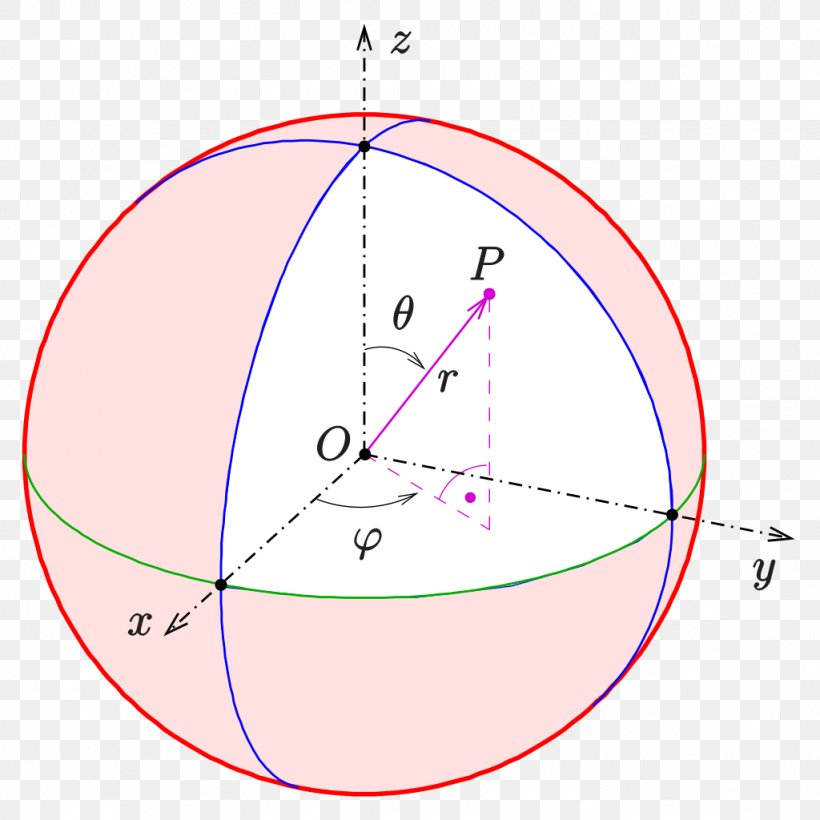
\includegraphics[width=\textwidth]{球坐标换元.png}
        \caption{球坐标换元}
        \label{fig:球坐标换元}
    \end{marginfigure}
        \begin{itemize}
            \item 雅可比行列式:$\frac{\partial(x,y,z)}{\partial(r,\theta,\varphi)}=r^2\cos(\varphi)$
            \item 参数范围:$(r,\theta,\varphi)\in(0,\infty)\times (-\pi,\pi)\times (-\frac{\pi}{2},\frac{\pi}{2})$
        \end{itemize}
\end{itemize}

\begin{kaobox}[frametitle=球坐标换元的说明]
    球坐标换元并不唯一,这里我们采用了\sidecite{于品}的定义,此外
    \[
        (x,y,z)=(r\cos(\varphi)\sin(\theta),r\sin(\varphi)\sin(\theta),r\cos(\theta))
    \]
    也是一个球坐标换元. 雅可比行列式为$r^2\sin(\theta)$. 参数取值范围为
    \[
        (r,\theta,\varphi)\in[0,\infty)\times[0,\pi)\times[0,2\pi)
    \]
\end{kaobox}

\subsection{Poisson公式和余面积公式}

球面外法向量:球面$(x-x_0)^2+(y-y_0)^2+(z-z_0)^2=r^2$在其上任意一点$(x,y,z)$的单位外法向量为
\[
    \left(\frac{x-x_0}{r},\frac{y-y_0}{r},\frac{z-z_0}{r}\right)
\]
\begin{theorem}[余面积公式]\label{thm:residual-area-formula}\marginnote{该公式串联了重积分、曲线积分、曲面积分,非常好用.}
    \begin{enumerate}
        \item \[\iint\limits_{r_1 \leqslant F(x, y) \leqslant r_2} f(x, y) \mathrm{d} x \mathrm{d} y=\int_{r_1}^{r_2} \mathrm{d} r \int_{F(x, y)=r} \frac{f(x, y)}{\sqrt{\left|\frac{\partial F}{\partial x}\right|^2+\left|\frac{\partial F}{\partial y}\right|^2}} \mathrm{d} s .\]
        \item \[\iiint\limits_{r_1 \leqslant F(x, y, z) \leqslant r_2} f(x, y, z) \mathrm{d} x \mathrm{d} y \mathrm{d} z=\int_{r_1}^{r_2} \mathrm{d} r \iint\limits_{F(x, y, z)=r} \frac{f(x, y, z)}{\sqrt{\left|\frac{\partial F}{\partial x}\right|^2+\left|\frac{\partial F}{\partial y}\right|^2+\left|\frac{\partial F}{\partial z}\right|^2}} \mathrm{d} S .\]
    \end{enumerate}
\end{theorem}

接下来展示一个利用余面积公式计算变态重积分的例子.

\begin{exercise}
计算
$$
\iiint\limits_{\Omega} \frac{1}{(1+x+y+z)^3} \mathrm{d} x \mathrm{d} y \mathrm{d} z,
$$
这里
$$
\Omega=\left\{(x, y, z) \in \mathbb{R}^3: x, y, z \geqslant 0, x+y+z \leqslant 1\right\} .
$$
\end{exercise}

\begin{solution}
    利用余面积公式\ref{thm:residual-area-formula},我们有
{\small
$$
\begin{aligned}
& \iiint\limits_{\Omega} \frac{1}{(1+x+y+z)^3} \mathrm{d} x \mathrm{d} y \mathrm{d} z=\iiint\limits_{x+y+z \leqslant 1} \frac{\chi_{[0,+\infty)^3}(x, y, z)}{(1+x+y+z)^3} \mathrm{d} x \mathrm{d} y \mathrm{d} z \\
& \quad=\frac{1}{\sqrt{3}} \int_{-\infty}^1 \mathrm{d} r \iint\limits_{x+y+z=r} \frac{\chi_{[0,+\infty)^3}(x, y, z)}{(1+x+y+z)^3} \mathrm{d} S=\frac{1}{\sqrt{3}} \int_0^1 \mathrm{d} r \iint\limits_{x+y+z=r} \frac{\chi_{[0,+\infty)^3}(x, y, z)}{(1+r)^3} \mathrm{d} S \\
& \quad=\frac{1}{\sqrt{3}} \int_0^1 \frac{1}{(1+r)^3} \mathrm{d} r \iint\limits_{x+y+z=r, x, y, z \geqslant 0} 1 \mathrm{d} S=\frac{1}{2} \int_0^1 \frac{r^2}{(1+r)^3} \mathrm{d} r=\frac{\ln 2}{2}-\frac{5}{16} .
\end{aligned}
$$
}
\end{solution}

作为多元积分换元法的应用,我们有Poisson公式\sidenote[][-1mm]{Poisson公式本质上依赖于还原法,所以实际运用中要注意变通,并不仅仅适用于上述形式. 此外Poisson公式在一些常见例题中,右端项还可以进一步简化为单变量积分,那样不利于记忆,这里给出便于记忆的形式. 而且,Poisson公式对于$n$重积分和$n$重曲面积分也是正确的.}.

\begin{theorem}[二元函数Poisson公式]
    设 $r>0, a, b, c \in \mathbb{R}$, 且下述积分有意义, 则有
{\small
\begin{align}
    \iint\limits_{x^2+y^2 \leqslant r^2} f(a x+b y) g\left(x^2+y^2\right) \mathrm{d} x \mathrm{d} y & =\iint\limits_{x^2+y^2 \leqslant r^2} f\left(\sqrt{a^2+b^2} y\right) g\left(x^2+y^2\right) \mathrm{d} x \mathrm{d} y \\
    \oint\limits_{x^2+y^2=r^2} f(a x+b y) g\left(x^2+y^2\right) \mathrm{d} s & =\oint\limits_{x^2+y^2=r^2} f\left(\sqrt{a^2+b^2} y\right) g\left(x^2+y^2\right) \mathrm{d} s .
\end{align}
}
\end{theorem}

\begin{theorem}[三元函数Poisson公式]
    设 $r>0, a, b, c \in \mathbb{R}$, 且下述积分有意义, 则有
{\small 
\begin{equation}
    \begin{split}
        & \iiint\limits_{x^2+y^2+z^2 \leqslant r^2}  f(a x+b y+c z) g\left(x^2+y^2+z^2\right) \mathrm{d} x \mathrm{d} y \mathrm{d} z \\
        = & \iiint\limits_{x^2+y^2+z^2 \leqslant r^2} f\left(\sqrt{a^2+b^2+c^2} z\right) g\left(x^2+y^2+z^2\right) \mathrm{d} x \mathrm{d} y \mathrm{d} z 
    \end{split}
\end{equation}
\begin{equation}
    \begin{split}
        & \iint\limits_{x^2+y^2+z^2=r^2}  f(a x+b y+c z) g\left(x^2+y^2+z^2\right) \mathrm{d} S \\
        = & \iint\limits_{x^2+y^2+z^2=r^2} f\left(\sqrt{a^2+b^2+c^2} z\right) g\left(x^2+y^2+z^2\right) \mathrm{d} S
    \end{split}
\end{equation}
}   
\end{theorem}

\begin{exercise}
    设$a,b,c\in\mathbb{R}\setminus\{0\}$,计算
    \[
        \iiint\limits_{x^2+y^2+z^2\leq r^2} (x^2+y^2+z^2)^p\left|ax+by+cz\right|^q\mathrm{d}x\mathrm{d}y\mathrm{d}z
    \]\marginnote{如何判断广义重积分的收敛性?直接加上绝对值爆算,算出来收敛就收敛,算出来发散就发散.}
\end{exercise}

\begin{solution}
    直接计算有
    \begin{align*}
        &\iiint\limits_{x^2+y^2+z^2\leq r^2} (x^2+y^2+z^2)^p\left|ax+by+cz\right|^q\mathrm{d}x\mathrm{d}y\mathrm{d}z\\
        &\overset{\text{余面积公式}\ref{thm:residual-area-formula}}{=}\int_0^r t^{2p}\mathrm{d}t\iint\limits_{x^2+y^2+z^2=t^2} (x^2+y^2+z^2)^p\left|ax+by+cz\right|^q\mathrm{d}S\\
        &\overset{\text{Poisson公式}\ref{thm:second-type-surface-integral-change-of-variable}}{=}(a^2+b^2+c^2)^{q/2}\int_0^r t^{2p}\mathrm{d}t\iint\limits_{x^2+y^2+z^2=t^2} \left|z\right|^q\mathrm{d}S\\
        &=2(a^2+b^2+c^2)^{q/2}\int_0^r t^{2p}\mathrm{d}t\iint\limits_{x^2+y^2+z^2=t^2,z\ge 0} z^q\mathrm{d}S\\
        &\overset{\text{换元法}}{=}2(a^2+b^2+c^2)^{q/2}\int_0^r t^{2p+q+2}\mathrm{d}t\iint\limits_{x^2+y^2+z^2=1,z\ge 0} z^q\mathrm{d}S\\
        &=2(a^2+b^2+c^2)^{q/2}\int_0^r t^{2p+q+2}\mathrm{d}t\iint\limits_{x^2+y^2\le 1} (1-x^2-y^2)^{(q-1)/2}\mathrm{d}x\mathrm{d}y\\
        &\overset{\text{余面积公式}\ref{thm:residual-area-formula}}{=}2(a^2+b^2+c^2)^{q/2}\int_0^r t^{2p+q+2}\mathrm{d}t\int_0^1\mathrm{d}v\int_{x^2+y^2=v^2} (1-x^2-y^2)^{(q-1)/2}\mathrm{d}s\\
        &=4\pi(a^2+b^2+c^2)^{q/2}\int_0^r t^{2p+q+2}\mathrm{d}t\int_0^1 v(1-v^2)^{(q-1)/2}\mathrm{d}v\\
    \end{align*}
    因此积分收敛等价于
    \[
    2p+q+2>-1,\quad \frac{q-1}{2}>-1
    \]
    于是积分收敛时,有
    \[
    \iiint\limits_{x^2+y^2+z^2\leq r^2} (x^2+y^2+z^2)^p\left|ax+by+cz\right|^q\mathrm{d}x\mathrm{d}y\mathrm{d}z=\frac{4\pi}{2p+q+3}(a^2+b^2+c^2)^{q/2}r^{2p+q+3}(q+1)
    \]
\end{solution}

\begin{exercise}
    计算积分
    \[
        L=\iiint_{(T)}\left(\frac{x^2}{a^2}+\frac{y^2}{b^2}+\frac{z^2}{c^2}\right) \mathrm{d}x\mathrm{d}y\mathrm{d}z
    \]
    其中$(T)$是整个椭球体$\frac{x^2}{a^2}+\frac{y^2}{b^2}+\frac{z^2}{c^2} \leqslant 1$.
\end{exercise}

\begin{solution}
    应用投影法,得
    \[
        L=\int_{-a}^a \frac{x^2}{a^2} \mathrm{d}x \iint_{(P_x)} \mathrm{d}y\mathrm{d}z+\int_{-b}^b \frac{y^2}{b^2} \mathrm{d}y \iint_{(Q_y)} \mathrm{d}z\mathrm{d}x+\int_{-c}^c \frac{z^2}{c^2} \mathrm{d}z \iint_{(R_z)} \mathrm{d}x\mathrm{d}y
    \]
    于是,
    \begin{align*}
        L &= \frac{\pi bc}{a^2} \int_{-a}^a x^2\left(1-\frac{x^2}{a^2}\right) \mathrm{d}x+\frac{\pi ca}{b^2} \int_{-b}^b y^2\left(1-\frac{y^2}{b^2}\right) \mathrm{d}y \\
        &\quad +\frac{\pi ab}{c^2} \int_{-c}^c z^2\left(1-\frac{z^2}{c^2}\right) \mathrm{d}z \\
        &= \frac{4}{5} \cdot \pi abc
    \end{align*}
\end{solution}


\section{投影法}

用于计算第二型曲面积分. 第二型曲面积分不同于第一型,它是有向的. 如下等式揭示了这两者的关系:
\[
    \iint_S Pdxdy+Qdydz+Rdzdx=\iint_S P\cos\alpha+Q\cos\beta+R\cos\gamma\mathrm{d}S
\]
其中$(\cos\alpha,\cos\beta,\cos\gamma)$是曲面$S$在点$(x,y,z)$处的法向量的方向余弦,给出了曲面$S$的那一侧.

根据上述讨论,我们已经可以将第二型曲面积分转化为第一型曲面积分,不过下面的定理(投影法)表明,可以直接把第二型曲面积分化为二重积分进行计算.
\begin{theorem}[投影法]
    设$R(x,y,z)$在光滑曲面
    $$
    S:z=z(x,y), (x,y)\in D
    $$
    上连续,则
    $$
    \iint_S R(x,y,z)dxdy=\pm \iint_D R(x,y,z(x,y))dxdy
    $$
    其中$S$表示上侧时取正号,$S$表示下侧时取负号.
\end{theorem}

\section{重积分换元技巧}

换元并不一定是标准换元,换元技巧是多样的.

\begin{exercise}
    计算曲面
    \[
        \left(\frac{x}{a}\right)^{2/3}+\left(\frac{y}{b}\right)^{2/3}+\left(\frac{z}{c}\right)^{2/3}=1
    \]
    所围立体的体积.
\end{exercise}

\begin{solution}
    按下面公式引入新的坐标:
    $$
    \begin{aligned}
    x= & a r \sin ^3 \varphi \cos ^3 \theta, y=b r \sin ^3 \varphi \sin ^3 \theta, z=c r \cos ^3 \varphi \\
    & (0 \leqslant r \leqslant 1,0 \leqslant \varphi \leqslant \pi, 0 \leqslant \theta \leqslant 2 \pi)
    \end{aligned}
    $$
    这时雅可比式
    $$
    J=9 a b c r^2 \sin ^5 \varphi \cos ^2 \varphi \sin ^2 \theta \cos ^2 \theta,
    $$
    所以

    $$
    V=9 a b c \int_0^1 r^2 d r \int_0^\pi \sin ^5 \varphi \cos ^2 \varphi d \varphi \int_0^{2 \pi} \sin ^2 \theta \cos ^2 \theta d \theta=\frac{4}{35} \pi a b c .
    $$
\end{solution}

\begin{exercise}
    求曲面
    \[
        (x+y+z)^2=a y, x=0, y=0, z=0
    \]
    所围立体的体积.
\end{exercise}

\begin{solution}
    令
    $$
    \begin{aligned}
    x= & r \sin ^2 \varphi \cos ^2 \theta, y=r \sin ^2 \varphi \sin ^2 \theta, z=r \cos ^2 \varphi \\
    & \left(r \geqslant 0,0 \leqslant \varphi \leqslant \frac{\pi}{2}, 0 \leqslant \theta \leqslant \frac{\pi}{2}\right)
    \end{aligned}
    $$
    这时雅可比式
    $$
    J=4 r^2 \sin ^3 \varphi \cos \varphi \sin \theta \cos \theta
    $$
    代入原方程$(x+y+z)^2=ay$得:
    $$
    (r\sin^2\varphi\cos^2\theta + r\sin^2\varphi\sin^2\theta + r\cos^2\varphi)^2 = ar\sin^2\varphi\sin^2\theta
    $$
    即
    $$
    r^2 = ar\sin^2\varphi\sin^2\theta
    $$
    所以$r = a\sin^2\varphi\sin^2\theta$,因此体积为$V = \frac{a^3}{60}$.
\end{solution}

\begin{exercise}
    计算逐次积分
    $$
    \int_1^{\infty} d z \int_1^{\infty} y d y \int_0^{\frac{1}{y z}} e^{x y z} x^2 d x
    $$
\end{exercise}

\begin{solution}
    将它换作三重积分
    $$
    \iiint_{\substack{x \geqslant 0, y, z \geqslant 1 \\ x y z \leqslant 1}} e^{x y z} x^2 y d x d y d z,
    $$
    再采用替换
    $$
    x=u, \quad y=\frac{u+v}{u}, \quad z=\frac{u+v+w}{u+v}, \quad J=\frac{1}{u(u+v)} .
    $$
    积分化为:
    $$
    \iiint_{\substack{u, v, w \geqslant 0 \\ u+v+w \leqslant 1}} e^{u+v+w} d u d v d w
    $$
    这很容易计算,结果为$\frac{e}{2}-1$.
\end{solution}

\begin{exercise}
    计算积分
    $$
    H=\iiint_{\substack{x, y, z \geqslant 0 \\ x^2+y^2+z^2 \leqslant R^2}} \frac{x y z d x d y d z}{\sqrt{\alpha^2 x^2+\beta^2 y^2+\gamma^2 z^2}} \quad(\alpha>\beta>\gamma>0)
    $$
\end{exercise}

\begin{solution}
    在球坐标下
    $$
    H=\int_0^{\frac{\pi}{2}} \int_0^{\frac{\pi}{2}} \int_0^R \frac{r^4 \sin ^3 \varphi \cos \varphi \sin \theta \cos \theta d r d \varphi d \theta}{\sqrt{\alpha^2 \sin ^2 \varphi \cos ^2 \theta+\beta^2 \sin ^2 \varphi \sin ^2 \theta+\gamma^2 \cos ^2 \varphi}} .
    $$
    进行替换 $\sin ^2 \varphi=u, \sin ^2 \theta=v$ 较为方便. 则
    $$
    \begin{aligned}
    H & =\frac{1}{4} \int_0^1 \int_0^1 \int_0^R r^4 \frac{u d r d u d v}{\sqrt{\alpha^2 u(1-v)+\beta^2 u v+\gamma^2(1-u)}} \\
    & =\frac{R^5}{20} \int_0^1 u d u \int_0^1 \frac{d v}{\sqrt{\left[\gamma^2+\left(\alpha^2-\gamma^2\right) u\right]+\left(\beta^2-\alpha^2\right) u v}} \\
    & =\frac{R^5}{15} \frac{\beta \gamma+\gamma \alpha+\alpha \beta}{(\beta+\gamma)(\gamma+\alpha)(\alpha+\beta)} .
    \end{aligned}
    $$
\end{solution}

\section{三角函数积分}

计算:
\[
    \int_0^{\pi/2}\sin^n x dx=\begin{cases}
        \frac{(n-1)!!}{n!!}\cdot\frac{\pi}{2},&n\text{为偶数}\\
        \frac{(n-1)!!}{n!!},&n\text{为奇数}
    \end{cases}
\]
\begin{solution}
    令$I_n=\int_0^{\pi/2}\sin^n x dx$,则有
    \begin{align*}
        I_n &= \int_0^{\pi/2}\sin^n x dx = \int_0^{\pi/2}\sin^{n-1} x \sin x dx \\
        &= \int_0^{\pi/2}\sin^{n-1} x d(\cos x) \\
        &= -\cos x \sin^{n-1} x \Big|_0^{\pi/2} + (n-1)\int_0^{\pi/2}\sin^{n-2} x (1-\cos^2 x) dx \\
        &= (n-1)I_{n-2}-(n-1)I_n
    \end{align*}
    于是
    \[
        I_n=\frac{n-1}{n}I_{n-2},\quad I_0=\frac{\pi}{2},I_1=1
    \]
    递推下去,当$n$为偶数时,$I_n = \frac{(n-1)!!}{n!!}\cdot\frac{\pi}{2}$,当$n$为奇数时,$I_n = \frac{(n-1)!!}{n!!}$.
\end{solution}

\section{特殊函数}

\begin{definition}[Gamma函数]
    Gamma函数定义为
    $$
    \Gamma(x) = \int_0^\infty t^{x-1}e^{-t}\mathrm{d}t
    $$
\end{definition}

\begin{theorem}[Gamma函数的性质]
    Gamma函数满足以下性质:
    \begin{enumerate}
        \item $\Gamma(x+1) = x\Gamma(x)$
        \item $\Gamma(n) = (n-1)!,\forall n\in\mathbb{N}$
        \item $\Gamma\left(\frac{1}{2}\right) = \sqrt{\pi}$
        \item $\Gamma(x)\Gamma(1-x) = \frac{\pi}{\sin(x\pi)},\forall x\in(0,1)$\sidenote{余元公式.}
    \end{enumerate}
\end{theorem}

\begin{definition}[Beta函数]
    Beta函数定义为
    $$
    B(x,y) = \int_0^1 t^{x-1}(1-t)^{y-1}\mathrm{d}t=\frac{\Gamma(x)\Gamma(y)}{\Gamma(x+y)}
    $$
\end{definition}

\begin{theorem}[Beta函数的性质]
    Beta函数满足以下性质:
    \begin{enumerate}
        \item $B(x,y) = B(y,x)$
        \item $B(x,y) = \int_0^\infty \frac{u^{x-1}}{(1+u)^{x+y}}\mathrm{d}u$\sidenote{换元令$t=\frac{u}{1+u}$即可得到}
        \item $B(x,y) = \frac{\Gamma(x)\Gamma(y)}{\Gamma(x+y)}$
        \item $B(x,1-x) = \frac{\pi}{\sin(x\pi)},\forall x\in(0,1)$\sidenote{余元公式.}
        \item $B(x,y)={\color{red}2}\int_0^{\pi/2}\sin^{2x-1}\theta\cos^{2y-1}\theta\mathrm{d}\theta$\sidenote{令$t=\sin^2\theta$换元.}
        \item $B\left(\frac{1}{2},\frac{1}{2}\right) = \pi$
    \end{enumerate}
\end{theorem}

\begin{exercise}
    证明: 对任意 $p>0$ 都有
$$
\int_0^{\frac{\pi}{2}} \sin ^p x \mathrm{~d} x=\int_0^{\frac{\pi}{2}} \cos ^p x \mathrm{~d} x=\frac{1}{2} \mathrm{~B}\left(\frac{1}{2}, \frac{p+1}{2}\right) .
$$
并据此计算当 $p$ 为正整数时的积分值.
\end{exercise}
\begin{exercise}
    证明: $\lim _{n \rightarrow \infty} \int_0^{+\infty} \mathrm{e}^{-x^n} \mathrm{~d} x=1$.
\end{exercise}

\section{曲线积分与曲面积分}

设曲面 $S$ 的参数方程为
$$
x=x(u, v), \quad y=y(u, v), \quad z=z(u, v), \quad(u, v) \in D,
$$
其中, $D$ 是平面上一个具有连续边界的有界闭区域, $x(u, v), y(u, v)$ 和 $z(u, v)$ 都是区域 $D$ 上的连续可微函数, 使得矩阵
$$
\left(\begin{array}{lll}
x_u & y_u & z_u \\
x_v & y_v & z_v
\end{array}\right)
$$
在 $D$ 上每个点处的秩都是 2 . 又设 $f(x, y, z)$ 是定义在曲面 $S$ 上的连续函数. 则 $f$ 在 $S$ 上可积, 且
\begin{align*}
\iint f(x, y, z) \mathrm{d} \sigma &= \iint f(x(u, v), y(u, v), z(u, v)) \\
&\quad \times \sqrt{\left|\frac{\partial(x, y)}{\partial(u, v)}\right|^2+\left|\frac{\partial(y, z)}{\partial(u, v)}\right|^2+\left|\frac{\partial(z, x)}{\partial(u, v)}\right|^2} \mathrm{~d} u \mathrm{~d} v
\end{align*}

\begin{theorem}[第二型曲线积分与第一型曲线积分的关系]
    设 $C$ 是连续可微的有向曲线, 它在其上点 $(x, y, z)$ 处的单位切向量为 $\boldsymbol{v}(x, y, z)$. 又设 $\boldsymbol{F}(x, y, z)$ 是定义在曲线 $C$ 上的向量函数. 则有
    $$
    \int_C \boldsymbol{F}(x, y, z) \cdot \mathrm{d} \boldsymbol{r}=\int_C \boldsymbol{F}(x, y, z) \cdot \boldsymbol{v}(x, y, z) \mathrm{d} s .
    $$
    即 $\boldsymbol{F}(x, y, z)$ 沿曲线 $C$ 的第二型曲线积分等于它与 $C$ 的单位切向量函数 $\boldsymbol{v}(x, y, z)$ 的内积 $\boldsymbol{F}(x, y, z) \cdot \boldsymbol{v}(x, y, z)$ 在 $C$ 上的第一型曲线积分.
\end{theorem}

\begin{theorem}[第二型曲面积分与第一型曲面积分的关系]
    设有向曲面 $S$ 的参数方程为
    $$
    x=x(u, v), \quad y=y(u, v), \quad z=z(u, v), \quad(u, v) \in D,
    $$
    其中, $D$ 是平面上一个具有连续边界的有界闭区域, $x(u, v), y(u, v)$ 和 $z(u, v)$ 都是区域 $D$ 上的连续可微函数, 使得矩阵
    $$
    \left(\begin{array}{lll}
    x_u & y_u & z_u \\
    x_v & y_v & z_v
    \end{array}\right)
    $$
    在 $D$ 上每个点处的秩都是 2. 又设 $\boldsymbol{F}(x,y,z)$ 是定义在曲面 $S$ 上的向量函数. 则有
    $$
    \iint_S \boldsymbol{F}(x,y,z) \cdot \mathrm{d}\boldsymbol{S} = \iint_S \boldsymbol{F}(x,y,z) \cdot \boldsymbol{n}(x,y,z) \mathrm{d}\sigma,
    $$
    其中 $\boldsymbol{n}(x,y,z)$ 是曲面 $S$ 在点 $(x,y,z)$ 处的单位法向量.
\end{theorem}

\begin{theorem}[第二型曲面积分正负号的确定]\label{第二型曲面积分正负号的确定}
    设有向曲面 $S$ 的参数方程为
    $$
    x=x(u, v), \quad y=y(u, v), \quad z=z(u, v), \quad(u, v) \in D,
    $$
    其中, $D$ 是平面上一个具有连续边界的有界闭区域, $x(u, v), y(u, v)$ 和 $z(u, v)$ 都是区域 $D$ 上的连续可微函数, 使得矩阵
    $$
    \left(\begin{array}{lll}
    x_u & y_u & z_u \\
    x_v & y_v & z_v
    \end{array}\right)
    $$
    在 $D$ 上每个点处的秩都是 2. 又设 $\boldsymbol{F}(x, y, z)$ 是定义在曲面 $S$ 上的连续向量函数, 其分量表达式为
    $$
    \boldsymbol{F}(x, y, z)=P(x, y, z) \boldsymbol{i}+Q(x, y, z) \boldsymbol{j}+R(x, y, z) \boldsymbol{k} .
    $$
    则有
    $$
    \iint_S \boldsymbol{F}(x,y,z) \cdot \mathrm{d}\boldsymbol{S} = \iint_D \left|\begin{array}{ccc}
    P & Q & R \\
    x_u & y_u & z_u \\
    x_v & y_v & z_v
    \end{array}\right| \mathrm{d}u\mathrm{d}v.
    $$
    其中, $P(u, v)=P(x(u, v), y(u, v), z(u, v)), Q(u, v)=Q(x(u, v), y(u, v), z(u, v))$,$ R(u, v)=R(x(u, v), y(u, v), z(u, v))$. 等式右端正负号的选取规则为当 $S$ 的给定法向量 $\boldsymbol{n}$ 与向量 $\boldsymbol{r}_u \times \boldsymbol{r}_v$ (其中 $\boldsymbol{r}=x(u, v) \boldsymbol{i}+y(u, v) \boldsymbol{j}+z(u, v) \boldsymbol{k}$) 同向时取正号, 反向时则取负号.
\end{theorem}

设有向曲面 $S$ 的参数方程为
$$
x=x(u, v), \quad y=y(u, v), \quad z=z(u, v), \quad(u, v) \in D,
$$
其中, $D$ 是平面上一个具有连续边界的有界闭区域, $x(u, v), y(u, v)$ 和 $z(u, v)$ 都是区域 $D$ 上的连续可微函数, 使得矩阵
$$
\left(\begin{array}{lll}
x_u & y_u & z_u \\
x_v & y_v & z_v
\end{array}\right)
$$
在 $D$ 上每个点处的秩都是 2 . 又设 $f(x, y, z)$ 是定义在曲面 $S$ 上的连续函数. 则有
$$
\begin{aligned}
& \iint_S f(x, y, z) \mathrm{d} y \mathrm{~d} z= \pm \iint_D f(x(u, v), y(u, v), z(u, v)) \frac{\partial(y, z)}{\partial(u, v)} \mathrm{d} u \mathrm{~d} v \\
& \iint_S f(x, y, z) \mathrm{d} z \mathrm{~d} x= \pm \iint_D f(x(u, v), y(u, v), z(u, v)) \frac{\partial(z, x)}{\partial(u, v)} \mathrm{d} u \mathrm{~d} v \\
& \iint_S f(x, y, z) \mathrm{d} x \mathrm{~d} y= \pm \iint_D f(x(u, v), y(u, v), z(u, v)) \frac{\partial(x, y)}{\partial(u, v)} \mathrm{d} u \mathrm{~d} v .
\end{aligned}
$$
这里正负号的选取规则如定理\ref{第二型曲面积分正负号的确定}所述.

特别地,如果曲面 $S$ 是由显式方程
$$
z=\varphi(x, y), \quad(x, y) \in D
$$
给出,其中, $D$ 是平面上具连续边界的有界闭区域, $f(x, y)$ 是定义在区域 $D$ 上的一阶连续可微函数,且 $S$ 的正向指向曲面的上方,则应用以上公式可知
$$
\begin{aligned}
& \iint_S f(x, y, z) \mathrm{d} y \mathrm{~d} z=-\iint_D f(x, y, \varphi(x, y)) \varphi_x(x, y) \mathrm{d} x \mathrm{~d} y \\
& \iint_S f(x, y, z) \mathrm{d} z \mathrm{~d} x=-\iint_D f(x, y, \varphi(x, y)) \varphi_y(x, y) \mathrm{d} x \mathrm{~d} y \\
& \iint_S f(x, y, z) \mathrm{d} x \mathrm{~d} y=\iint_D f(x, y, \varphi(x, y)) \mathrm{d} x \mathrm{~d} y
\end{aligned}
$$
与第二型曲线积分类似,对于第二型曲面积分,改变曲面的定向就改变了积分的正负号,即
$$
\begin{aligned}
& \iint_{S^{-}} P(x, y, z) \mathrm{d} y \mathrm{~d} z+Q(x, y, z) \mathrm{d} z \mathrm{~d} x+R(x, y, z) \mathrm{d} x \mathrm{~d} y \\
= & -\iint_S P(x, y, z) \mathrm{d} y \mathrm{~d} z+Q(x, y, z) \mathrm{d} z \mathrm{~d} x+R(x, y, z) \mathrm{d} x \mathrm{~d} y,
\end{aligned}
$$
其中 $S^{-}$表示把 $S$ 的方向改变为反方向所得到的有向曲面。这是第二型曲面积分与第一型曲面积分的一个重要区别。
\begin{example}
计算第二型曲面积分
$$
I=\iint_S \frac{\mathrm{~d} y \mathrm{~d} z}{x}+\frac{\mathrm{d} z \mathrm{~d} x}{y}+\frac{\mathrm{d} x \mathrm{~d} y}{z},
$$
其中 $S$ 是椭球面 $\frac{x^2}{a^2}+\frac{y^2}{b^2}+\frac{z^2}{c^2}=1$, 以外侧为正侧.
\end{example}

\begin{solution}
    利用对称性,只需计算三个积分中的任何一个. 下面以第三个积分 $I_3$ 为例来计算。椭球面 $S$ 分为上、下两半,分别记为 $S_1$ 和 $S_2$ 。因为 $S_1$ 以上侧为正向, $S_2$ 以下侧为正向,所以
$$
\begin{aligned}
I_3 & =\iint_{S_1} \frac{\mathrm{~d} x \mathrm{~d} y}{z}+\iint_{S_2} \frac{\mathrm{~d} x \mathrm{~d} y}{z} \\
& =\iint_D \frac{\mathrm{~d} x \mathrm{~d} y}{c \sqrt{1-\frac{x^2}{a^2}-\frac{y^2}{b^2}}}-\iint_D \frac{\mathrm{~d} x \mathrm{~d} y}{-c \sqrt{1-\frac{x^2}{a^2}-\frac{y^2}{b^2}}}=\frac{2}{c} \iint_D \frac{\mathrm{~d} x \mathrm{~d} y}{\sqrt{1-\frac{x^2}{a^2}-\frac{y^2}{b^2}}},
\end{aligned}
$$
其中 $D$ 是平面上的椭圆形区域 $\frac{x^2}{a^2}+\frac{y^2}{b^2} \leqslant 1$. 作广义极坐标变换 $x=\operatorname{ar} \cos \theta, y=$ $b r \sin \theta$ ,便有
$$
I_3=\frac{2}{c} \int_0^{2 \pi} \int_0^1 \frac{a b r}{\sqrt{1-r^2}} \mathrm{~d} r \mathrm{~d} \theta=\left.\frac{4 \pi a b}{c}\left(-\sqrt{1-r^2}\right)\right|_0 ^1=\frac{4 \pi a b}{c} .
$$
由对称性有
$$
I_1=\frac{4 \pi b c}{a}, \quad I_2=\frac{4 \pi a c}{b}
$$
因此
$$
I=I_1+I_2+I_3=\frac{4 \pi}{a b c}\left(a^2 b^2+a^2 c^2+b^2 c^2\right) .
$$
\end{solution}

\section{各种积分之间的联系与场论初步}

参考\cite{邓东皋},\cite{崔尚斌}.

\subsection{格林公式}
\begin{theorem}[\textcolor{green}{格林公式}]\label{格林公式}
设 $D$ 是由逐段光滑闭曲线 $L$ 围成的平面单连通闭区域, 函数 $P(x, y), Q(x, y)$ 在 $D$ 上有一阶连续偏导数, 则有
$$
\iint_D\left(\frac{\partial Q}{\partial x}-\frac{\partial P}{\partial y}\right) \mathrm{d} x \mathrm{~d} y=\oint_L P \mathrm{d} x+Q \mathrm{~d} y .
$$
其中右端的积分路径是闭曲线 $L$, 方向取正向.
\end{theorem}
\begin{marginfigure}
    \centering
    \includegraphics[width=\textwidth]{Green.png}
    \caption{格林公式}
    \label{fig:格林公式}
\end{marginfigure}
回忆闭曲线正向的含义是,当一人沿着曲线 $L$ 走时,区域 $D$ 始终在他的左边.

格林公式\ref{格林公式}还可以用来计算曲线所围成区域的面积,公式如下
\[
|D|=\frac{1}{2}\oint_L x \mathrm{d} y-y \mathrm{d} x
\]
如果使用极坐标换元,则有
\[
|D|=\frac{1}{2}\oint_L r^2 \mathrm{d} \theta 
\]
\marginnote[*-1]{注意这里的$\theta$取值范围要根据实际情况而定,并不是简单的从$0$到$2\pi$}

\begin{corollary}[二维分部积分公式]
    设 $D$ 是平面上由一条或数条分段光滑的闭曲线围成的区域, $P, Q, U, V$ 是 $D$ 上的连续可微函数. 则有
$$
\iint_D\left(P \frac{\partial U}{\partial x}+Q \frac{\partial V}{\partial y}\right) \mathrm{d} x \mathrm{~d} y=\int_{\partial D} P U \mathrm{~d} y-Q V \mathrm{~d} x-\iint_D\left(U \frac{\partial P}{\partial x}+V \frac{\partial Q}{\partial y}\right) \mathrm{d} x \mathrm{~d} y .
$$
其中 $\partial D$ 的正向取为按 $D$ 右旋的方向.
\end{corollary}
\begin{proof}
    根据格林公式, 有 
    \begin{align*}
        & \iint_D\left(P \frac{\partial U}{\partial x}+Q \frac{\partial V}{\partial y}\right) \mathrm{d} x \mathrm{~d} y+\iint_D\left(U \frac{\partial P}{\partial x}+V \frac{\partial Q}{\partial y}\right) \mathrm{d} x \mathrm{~d} y \\
        = & \iint_D\left(\frac{\partial(P U)}{\partial x}+\frac{\partial(Q V)}{\partial y}\right) \mathrm{d} x \mathrm{~d} y=\int_{\partial D} P U \mathrm{~d} y-Q V \mathrm{~d} x .
    \end{align*}
\end{proof}

\begin{example}[计算曲线积分]\label{ex:格林公式}
    计算曲线积分
    $$
    I=\int_C \frac{x \mathrm{~d} y-y \mathrm{~d} x}{x^2+y^2}
    $$
    其中 $C$ 是逆时针旋转且不经过坐标原点的封闭分段光滑曲线. 考虑两种情况:
    \begin{enumerate}
        \item $C$ 包围的区域不包含坐标原点;
        \item $C$ 包围的区域包含坐标原点.
    \end{enumerate}
\end{example}

\begin{marginfigure}
    \centering
    \includegraphics[width=\textwidth]{Green_ex1.png}
    \caption{例\ref{ex:格林公式}中的$D / B_{\varepsilon}(0)$}
    \label{fig:格林公式ex1}
\end{marginfigure}

\begin{solution}
    用 $D$ 表小 $C$ 包围的区域. 则当 $D$ 不包含坐标原点时, 函数 $P(x, y)=-\frac{y}{x^2+y^2}$ 和 $Q(x, y)=\frac{x}{x^2+y^2}$ 都在 $D$ 中连续可微. 因此应用格林公式得
$$
\begin{aligned}
\int_C \frac{x \mathrm{~d} y-y \mathrm{~d} x}{x^2+y^2} & =\iint_D\left[\frac{\partial}{\partial x}\left(\frac{x}{x^2+y^2}\right)-\frac{\partial}{\partial y}\left(\frac{-y}{x^2+y^2}\right)\right] \mathrm{d} x \mathrm{~d} y \\
& =\iint_D\left(\frac{y^2-x^2}{\left(x^2+y^2\right)^2}+\frac{x^2-y^2}{\left(x^2+y^2\right)^2}\right) \mathrm{d} x \mathrm{~d} y=0 .
\end{aligned}
$$
当 $D$ 包含坐标原点时, 因原点是函数 $P(x, y)=-\frac{y}{x^2+y^2}$ 和 $Q(x, y)=\frac{x}{x^2+y^2}$ 的奇点, 即 $P$ 和 $Q$ 不可微因而不满足格林公式条件的点, 所以不能直接应用格林公式. 这时取 $\varepsilon>0$ 充分小使闭圆盘 $\overline{B_{\varepsilon}(0)}$ 包含于 $D^{\circ}$ (图 20-3-5). 在区域 $D \backslash B_{\varepsilon}(0)$ 上应用格林公式得
$$
\begin{aligned}
\int_C \frac{x \mathrm{~d} y-y \mathrm{~d} x}{x^2+y^2} & =\iint_{D \backslash B_{\varepsilon}(0)}\left[\frac{\partial}{\partial x}\left(\frac{x}{x^2+y^2}\right)-\frac{\partial}{\partial y}\left(\frac{-y}{x^2+y^2}\right)\right] \mathrm{d} x \mathrm{~d} y+\int_{\partial B_{\varepsilon}(0)} \frac{x \mathrm{~d} y-y \mathrm{~d} x}{x^2+y^2} \\
& =\frac{1}{\varepsilon^2} \int_{\partial B_{\varepsilon}(0)} x \mathrm{~d} y-y \mathrm{~d} x
\end{aligned}
$$
对最后这个积分再次应用格林公式,就得到
$$
\begin{aligned}
\int_C \frac{x \mathrm{~d} y-y \mathrm{~d} x}{x^2+y^2} & =\frac{1}{\varepsilon^2} \iint_{B_{\varepsilon}(0)}\left(\frac{\partial x}{\partial x}-\frac{\partial(-y)}{\partial y}\right) \mathrm{d} x \mathrm{~d} y \\
& =\frac{2}{\varepsilon^2} \iint_{B_{\varepsilon}(0)} \mathrm{d} x \mathrm{~d} y=\frac{2}{\varepsilon^2} \cdot \pi \varepsilon^2=2 \pi
\end{aligned}
$$
\end{solution}



\subsection{高斯公式}
\begin{theorem}[高斯公式]\label{thm:gauss}
设空间区域 $V$ 由分片光滑的双侧封闭曲面 $S$ 围成,函数 $P(x, y, z), Q(x, y, z), R(x, y, z)$ 在 $V$ 及 $S$ 上有一阶连续偏导数, 则有
$$
\iiint_V\left(\frac{\partial P}{\partial x}+\frac{\partial Q}{\partial y}+\frac{\partial R}{\partial z}\right) \mathrm{d} x \mathrm{~d} y \mathrm{~d} z=\oiint_S P \mathrm{~d} y \mathrm{~d} z+Q \mathrm{~d} z \mathrm{~d} x+R \mathrm{~d} x \mathrm{~d} y,
$$
其中 $S$ 的方向为外侧.
\end{theorem}
\begin{corollary}[三维分部积分公式]
    设 $\Omega$ 是 $\mathbf{R}^3$ 中具有连续边界的有界闭区域, $P, Q, R, U, V, W$ 都是 $\Omega$ 上的连续可微函数. 则有
$$
\begin{aligned}
& \iiint_{\Omega}\left(P \frac{\partial U}{\partial x}+Q \frac{\partial V}{\partial y}+R \frac{\partial W}{\partial z}\right) \mathrm{d} x \mathrm{~d} y \mathrm{~d} z\\
= & \iint_{\partial \Omega}(P U \cos \alpha+Q V \cos \beta+R W \cos \gamma) \mathrm{d} \sigma \\
& -\iiint_{\Omega}\left(U \frac{\partial P}{\partial x}+V \frac{\partial Q}{\partial y}+W \frac{\partial R}{\partial z}\right) \mathrm{d} x \mathrm{~d} y \mathrm{~d} z .
\end{aligned}
$$
其中 $(\cos \alpha, \cos \beta, \cos \gamma)$ 是 $\Omega$ 边界的单位外法向量的方向余弦.
\end{corollary}
\begin{proof}
    应用高斯公式, 有
    {
        \small
        \begin{align*}
            & \iiint_{\Omega}\left(P \frac{\partial U}{\partial x}+Q \frac{\partial V}{\partial y}+R \frac{\partial W}{\partial z}\right) \mathrm{d} x \mathrm{~d} y \mathrm{~d} z+\iiint_{\Omega}\left(U \frac{\partial P}{\partial x}+V \frac{\partial Q}{\partial y}+W \frac{\partial R}{\partial z}\right) \mathrm{d} x \mathrm{~d} y \mathrm{~d} z \\
            = & \iiint_{\Omega}\left(\frac{\partial(P U)}{\partial x}+\frac{\partial(Q V)}{\partial y}+\frac{\partial(R W)}{\partial z}\right) \mathrm{d} x \mathrm{~d} y \mathrm{~d} z \\
            = & \iint_{\partial \Omega} P U \mathrm{~d} y \mathrm{~d} z+Q V \mathrm{~d} z \mathrm{~d} x+R W \mathrm{~d} x \mathrm{~d} y \\
            = & \iint_{\partial \Omega}(P U \cos \alpha+Q V \cos \beta+R W \cos \gamma) \mathrm{d} \sigma .
        \end{align*}
    }
\end{proof}

\subsection{斯托克斯公式}

\begin{theorem}[斯托克斯公式]
    若光滑曲面 $S$ 的边界为光滑曲线 $L$, 函数 $P, Q, R$ 在曲面 $S$ 及曲线 $L$ 上具有连续的一阶偏导数,则
    $$
    \begin{aligned}
    & \iint_S\left(\frac{\partial R}{\partial y}-\frac{\partial Q}{\partial z}\right) \mathrm{d} y \mathrm{~d} z+\left(\frac{\partial P}{\partial z}-\frac{\partial R}{\partial x}\right) \mathrm{d} z \mathrm{~d} x+\left(\frac{\partial Q}{\partial x}-\frac{\partial P}{\partial y}\right) \mathrm{d} x \mathrm{~d} y \\
    = & \oint_L P \mathrm{~d} x+Q \mathrm{~d} y+R \mathrm{~d} z
    \end{aligned}
    $$
    其中 $S$ 的侧与 $L$ 的方向按右手法则确定, 即若四个手指的方向为 $L$ 的方向,则大拇指所指的方向就是曲面 $S$ 的方向, 如图 22-13.
\end{theorem}

斯托克斯公式建立了函数在空间曲面 $S$ 上的第二型曲面积分与其 "原函数" 在 $S$ 的边界曲线 $L$ 上的第二型曲线积分之间的联系, 因此也是牛顿 - 莱布尼茨公式的一种高维的推广. 利用两种曲面积分之间的关系, 常把它写成如下便于记忆的形式:
$$
\begin{aligned}
\oint_L P \mathrm{~d} x+Q \mathrm{~d} y+R \mathrm{~d} z
& =\iint_S\left|\begin{array}{ccc}
\mathrm{d} y \mathrm{~d} z & \mathrm{~d} z \mathrm{~d} x & \mathrm{~d} x \mathrm{~d} y \\
\frac{\partial}{\partial x} & \frac{\partial}{\partial y} & \frac{\partial}{\partial z} \\
P & Q & R
\end{array}\right| \\
& =\iint_S\left|\begin{array}{ccc}
\cos \alpha & \cos \beta & \cos \gamma \\
\frac{\partial}{\partial x} & \frac{\partial}{\partial y} & \frac{\partial}{\partial z} \\
P & Q & R
\end{array}\right| \mathrm{d} S .
\end{aligned}
$$
不难看出,格林公式是斯托克斯公式的特殊情形。当 $L$ 是 $O x y$ 平面上的闭曲线时, $\mathrm{d} z=0$. 取 $S$ 为 $O x y$ 面上由 $L$ 围成的区域, 则 $S$ 在 $O_{y z}$ 和 $O_{z x}$ 平面上的投影为零, 因此对 $\mathrm{d} y \mathrm{~d} z, \mathrm{~d} z \mathrm{~d} x$ 的积分为 0 , 这时斯托克斯公式化为格林公式
$$
\oint_L P \mathrm{~d} x+Q \mathrm{~d} y=\iint_S\left|\begin{array}{cc}
\frac{\partial}{\partial x} & \frac{\partial}{\partial y} \\
P & Q
\end{array}\right| \mathrm{d} x \mathrm{~d} y .=\iint_S\left(\frac{\partial Q}{\partial x}-\frac{\partial P}{\partial y}\right) \mathrm{d} x \mathrm{~d} y .
$$

\begin{example}
    计算曲线积分
$$
\int_C\left(x^2-y z\right) \mathrm{d} x+\left(y^2-x z\right) \mathrm{d} y+\left(z^2-x y\right) \mathrm{d} z,
$$
其中 $C$ 是螺线 $x=a \cos \theta, y=a \sin \theta, z=b \theta$ 从点 $A(a, 0,0)$ 到点 $B(a, 0,2 \pi b)$ 的部分.
\end{example}

\begin{solution}
令 $S$ 是以由直线段 $A B$ 和曲线 $C$ 形成的封闭曲线为边界的任意光滑曲面,正侧为 $O z$ 轴的正向一侧. 则根据斯托克斯公式有
$$
\begin{aligned}
& \int_C\left(x^2-y z\right) \mathrm{d} x+\left(y^2-x z\right) \mathrm{d} y+\left(z^2-x y\right) \mathrm{d} z \\
& =\int_{\overline{A B}}\left(x^2-y z\right) \mathrm{d} x+\left(y^2-x z\right) \mathrm{d} y+\left(z^2-x y\right) \mathrm{d} z+\iint_S\left|\begin{array}{ccc}
\mathrm{d} y \mathrm{~d} z & \mathrm{~d} z \mathrm{~d} x & \mathrm{~d} x \mathrm{~d} y \\
\frac{\partial}{\partial x} & \frac{\partial}{\partial y} & \frac{\partial}{\partial z} \\
x^2-y z & y^2-x z & z^2-x y
\end{array}\right| \\
& =\int_0^{2 \pi b} z^2 \mathrm{~d} z=\frac{8}{3} \pi^3 b^3 .
\end{aligned}
$$
\end{solution}

\section{期末练习}

\begin{exercise}
    求 $\frac{\mathrm{d}}{\mathrm{d} x} \int_x^{x^2} \frac{\sin x y}{y} \mathrm{~d} y$, 其中 $x>0$.\marginnote{含参变量积分求导}
\end{exercise}
\begin{solution}
    利用\ref{thm:derivative-of-integral-with-parameter},我们有
    \begin{align*}
        ...=&\frac{2\sin x^3}{x^2}-\frac{\sin x^2}{x}+\int_x^{x^2}\cos(xy)\mathrm{d}y\\
        =&\frac{2\sin x^3}{x^2}-\frac{\sin x^2}{x}+\frac{\sin x^3}{x^2}-\frac{\sin x^2}{x}\\
        =&\frac{3\sin x^3}{x^2}-\frac{2\sin x^2}{x}
    \end{align*}
\end{solution}

\begin{exercise}
    利用Euler积分计算$\int_0^{\frac{\pi}{2}} \sin ^8 x \cos ^4 x \mathrm{~d} x$. 提示 $\Gamma(1 / 2)=\sqrt{\pi}$.\marginnote{使用Euler积分和Beta函数的性质}
\end{exercise}
\begin{solution}
    令$t=\sin^2x$,则有
    \begin{align*}
        \int_0^{\frac{\pi}{2}} \sin ^8 x \cos ^4 x \mathrm{~d} x&=\int_0^1 t^4(1-t)\cdot \frac{1}{2\sqrt{t(1-t)}}\mathrm{d}t\\
        &=\frac{B(\frac{9}{2},\frac{5}{2})}{2}=\frac{7\pi}{2^{11}}
    \end{align*}
\end{solution}
\begin{exercise}
    求圆锥面$z=\sqrt{x^2+y^2}$被$z^2=2x$截得的截面面积.\marginnote{直接使用投影法}
\end{exercise}
\begin{solution}
    考虑投影法投影到$Oxy$平面,则有
    \[
    dS=\sqrt{1+\left(\frac{\partial z}{\partial x}\right)^2+\left(\frac{\partial z}{\partial y}\right)^2}\mathrm{d}x\mathrm{d}y=\sqrt{1+1}\mathrm{d}x\mathrm{d}y
    \]
    联立$z=\sqrt{x^2+y^2}$和$z^2=2x$,可以得到$x^2+y^2=2x$,即$(x-1)^2+y^2=1$,因此这个投影是一个半径为1 的圆,面积为$\pi$,因此截面面积为$\pi\sqrt{2}$.所以积分
    \[
    \iint_S\mathrm{d}S=\iint_{x^2+y^2\leq 2x}\sqrt{1+1}\mathrm{d}x\mathrm{d}y=\sqrt{2}\pi
    \]
\end{solution}
\begin{exercise}
    设 $u=\mathrm{e}^x+x \sin y, v=\mathrm{e}^x-x \cos y$, 求 $\frac{\partial x}{\partial u} 、 \frac{\partial y}{\partial v}$ 。\marginnote{直接暴力求导}
\end{exercise}
\begin{solution}
对等式左右同时对 $u$ 求导得:
$$
\begin{cases}1= & \mathrm{e}^x \frac{\partial x}{\partial u}+\sin y \frac{\partial x}{\partial u}+x \cos y \frac{\partial y}{\partial u} \\ 0= & \mathrm{e}^x \frac{\partial x}{\partial u}-\cos y \frac{\partial x}{\partial u}+x \sin y \frac{\partial y}{\partial u}\end{cases}
$$
所以 $\sin y=\left[\left(\mathrm{e}^x+\sin y\right) \sin y-\left(\mathrm{e}^x-\cos y\right) \cos y\right] \frac{\partial x}{\partial u}$
$$
\frac{\partial x}{\partial u}=\frac{\sin y}{\mathrm{e}^x \sin y-\mathrm{e}^x \cos y+1}
$$
对等式左右同时对 $v$ 求导得:
$$
\begin{cases}0= & \mathrm{e}^x \frac{\partial x}{\partial v}+\sin y \frac{\partial x}{\partial v}+x \cos y \frac{\partial y}{\partial v} \\ 1= & \mathrm{e}^x \frac{\partial x}{\partial v}-\cos y \frac{\partial x}{\partial v}+x \sin y \frac{\partial y}{\partial v}\end{cases}
$$
所以 $-\cos y=\left(\mathrm{e}^x \sin y-\mathrm{e}^x \cos y+1\right) \frac{\partial x}{\partial v}$
$$
\begin{aligned}
& \frac{\partial x}{\partial v}=\frac{-\cos y}{\mathrm{e}^x \sin y-\mathrm{e}^x \cos y+1} \\
& \frac{\partial y}{\partial v}=\frac{\mathrm{e}^x+\sin y}{x\left(\mathrm{e}^x \sin y-\mathrm{e}^x \cos y+1\right)}
\end{aligned}
$$
\end{solution}
\begin{exercise}
    将三重积分 $\iiint_{\Omega} f(x, y, z) \mathrm{d} V$ 分别写成球坐标和柱坐标的三次积分的形式, 其中 $\Omega$ 是球 $x^2+y^2+(z-1)^2 \leqslant 1$ 和锥 $z \geqslant \sqrt{x^2+y^2}$ 的公共部分。\marginnote{球坐标和柱坐标换元,以及积分区域的确定}
\end{exercise}
\begin{solution}
\begin{enumerate}
    \item 球坐标:
    令 
    \[
    \left\{\begin{array}{l}x=r \cos \theta \\ y=r \sin \theta, \text { 其中 } \theta \in(0,2 \pi) \quad \varphi \in(0, \pi) \quad r \in(0,1), r \cos \varphi+1 \\ z=r\end{array}\right.
    \]
    因为 $z \geq \sqrt{x^2+y^2}$, 所以 $r \cos \varphi+1 \geq r \sin \varphi$
    $$
    r(\sin \varphi-\cos \varphi)=\sqrt{2} r \sin \left(\varphi-\frac{\pi}{4}\right) \leq 1
    $$
    若 $\varphi \in\left(0, \frac{\pi}{2}\right)$ 则 $r \in(0,1)$

    若 $\varphi \in\left(\frac{\pi}{2}, \pi\right)$ 则 $r \in\left(0, \frac{1}{\sin \varphi-\cos \varphi}\right)$
    所以
    $$
    \begin{aligned}
    \iiint_{\Omega} f(x, y, z) \mathrm{d} V& =\int_0^{2 \pi} \mathrm{~d} \theta \int_0^{\frac{\pi}{2}} \mathrm{~d} \varphi \int_0^1 f(r \cos \theta, r \sin \theta, r \cos \varphi+1) r^2 \sin \varphi \mathrm{~d} r \\
& +\int_0^{2 \pi} \mathrm{~d} \theta \int_{\frac{\pi}{2}}^\pi \mathrm{d} \varphi \int_0^{\frac{1}{\sin \varphi-\cos \varphi}} f(r \cos \theta, r \sin \theta, r \cos \varphi+1) r^2 \sin \varphi \mathrm{~d} r
\end{aligned}
$$
\item 柱坐标:

令 
\[\left\{\begin{array}{ll}
    x= & r \cos \theta \\
    y= & r \sin \theta
    \end{array} \text {, 其中 } \theta \in(0,2 \pi)\right.\]
则  $r^2+(z-1)^2  \leq 1   ,r   \leq z $

令 $1-(z-1)^2=z^2$, 解得 $z=0$ 或 $z=1$

所以 $0<z \leq 1$ 时, $1-(z-1)^2 \geq z^2 ; 1<z<2$ 时, $1-(z-1)^2<z^2$

所以
\begin{align*}
    \iiint_{\Omega} f(x, y, z) \mathrm{d} V&=\int_0^1 \mathrm{~d} z \int_0^{2 \pi} \mathrm{~d} \theta \int_0^z f(r \cos \theta, r \sin \theta, z) r \mathrm{~d} r\\
    &=\int_1^2 \mathrm{~d} z \int_0^{2 \pi} \mathrm{~d} \theta \int_0^{\sqrt{1-(z-1)^2}} f(r \cos \theta, r \sin \theta, z) r \mathrm{~d} r
\end{align*}    
\end{enumerate}
\end{solution}

\begin{exercise}
    求函数 $f(x, y)=\mathrm{e}^{2 x}\left(x+y^2+2 y\right)$ 的极值。\marginnote{函数极值的判断与验证(使用Hessian矩阵)}
\end{exercise}
\begin{solution}
    \[\begin{cases}
        \frac{\partial f}{\partial x}&=2 \mathrm{e}^{2 x}\left(x+y^2+2 y\right)+\mathrm{e}^{2 x}=\mathrm{e}^{2 x}\left(2 x+2 y^2+4 y+1\right)=0\\
        \frac{\partial f}{\partial y}&=\mathrm{e}^{2 x}(2 y+2)=0
    \end{cases}\]
解得 $\left\{\begin{array}{l}x=\frac{1}{2} \\ y-1\end{array}\right.$ 这是$f(x,y)$的唯一可能的极值点,接下来我们借助Hessian矩阵判断其是否为极值点,为什么类型的极值点。\sidenote{Hessian矩阵正定时,函数在该点取极小值;Hessian矩阵负定时,函数在该点取极大值;Hessian矩阵不定时,函数在该点不取极值,这个点是鞍点。\ref{thm:hessian-discrimination}}
\begin{align*}
    \frac{\partial^2 f}{\partial x^2}&=\mathrm{e}^{2 x}\left(4 x+4 y^2+8 y+4\right)=2 \mathrm{e}\\
    \frac{\partial^2 f}{\partial x \partial y}&=\mathrm{e}^{4 y+4}=0 \\
    \frac{\partial^2 f}{\partial y^2}&=2 \mathrm{e}^{2 x}=2 \mathrm{e}
\end{align*}
黑塞矩阵 $H=\left[\begin{array}{cc}2 \mathrm{e} & 0 \\ 0 & 2 \mathrm{e}\end{array}\right]$ 正定
所以原函数在 $\left(\frac{1}{2},-1\right)$ 处取极小值 $-\frac{\mathrm{e}}{2}$
\end{solution}

\begin{exercise}
    \marginnote{曲线积分参数化}求
    \[\int_L\left(x^{4/3}+y^{4/3}\right)\mathrm{d}s\]
    其中$L$为曲线$x^{2/3}+y^{2/3}=1$。
\end{exercise}
\begin{solution}
    换元令$x=\cos^3t,y=\sin^3t$,则有
    \[
        ds=\sqrt{\left(\frac{\partial x}{\partial t}\right)^2+\left(\frac{\partial y}{\partial t}\right)^2}\mathrm{d}t=\sqrt{9\cos^2t\sin^2t}\mathrm{d}t=3|\cos t\sin t|\mathrm{d}t
    \]
    同时
    \[
        x^{4/3}+y^{4/3}=\cos^4t+\sin^4t=\left(\cos^2t+\sin^2t\right)^2-2\cos^2t\sin^2t=1-2\cos^2t\sin^2t=1-\frac{1}{2}\sin^2(2t)
    \]
    于是
    \begin{align*}
        \int_L\left(x^{\frac{4}{3}}+y^{\frac{4}{3}}\right) d s= &\int_L\left(1-2 x^{\frac{2}{3}} y^{\frac{2}{3}}\right) d s \\
        = & \frac{3}{2} \int_0^{2 \pi}\left(2-\sin ^2 2 t\right)|\sin t \cos t| d t \\
        = & 4
    \end{align*}
\end{solution}
\begin{exercise}
    求
    \[
        \iint_\Omega u^3v^3\mathrm{d}u\mathrm{d}v
    \]
    其中$\Omega$是由$u=v^3,u=2v^3,u^3=v,u^3=2v,(u,v\ge 0)$所围成的区域.\marginnote{换元利用Jacobi行列式,为了简化运算,利用Jacobi矩阵的逆计算Jacobi行列式.}
\end{exercise}
\begin{solution}
    换元令$x=\frac{v^3}{u},y=\frac{u^3}{v},x\in[\frac{1}{2},1],y\in[1,2]$,则有\sidenote{
        利用
        \[
            \begin{pmatrix}
                \frac{\partial u}{\partial x}&\frac{\partial u}{\partial y}\\
                \frac{\partial v}{\partial x}&\frac{\partial v}{\partial y}
            \end{pmatrix}=\begin{pmatrix}
                \frac{\partial x}{\partial u}&\frac{\partial x}{\partial v}\\
                \frac{\partial y}{\partial u}&\frac{\partial y}{\partial v}
            \end{pmatrix}^{-1}
        \]
    }
    \[
        \mathrm{d}u\mathrm{d}v=\left|\begin{array}{cc}
        \frac{\partial x}{\partial u}&\frac{\partial x}{\partial v}\\
        \frac{\partial y}{\partial u}&\frac{\partial y}{\partial v}
        \end{array}\right|^{-1}\mathrm{d}x\mathrm{d}y=\left|\begin{array}{cc}
        -\frac{v^3}{u^2}&-\frac{3v^2}{u}\\
        \frac{3u^2}{v}&-\frac{u^3}{v^2}
        \end{array}\right|^{-1}\mathrm{d}x\mathrm{d}y=(8uv)^{-1}\mathrm{d}x\mathrm{d}y
    \]
    于是
    \[
        \iint_\Omega u^3v^3\mathrm{d}u\mathrm{d}v=\int_{\frac{1}{2}}^1\int_1^2\frac{u^3v^3}{8uv}\mathrm{d}x\mathrm{d}y=\frac{1}{8}\int_{\frac{1}{2}}^1\int_1^2 xy\mathrm{d}x\mathrm{d}y=\frac{9}{128}
    \]
\end{solution}

\begin{exercise}
    \marginnote{微分中值定理}设$u(x,y)$在区域$\Omega$内存在偏导数,且$u_x(x,y)=u_y(x,y)=0$,证明:$u(x,y)$在$\Omega$内恒为常数。
\end{exercise}
\begin{proof}
    由微分中值定理:
    \[
        u(x+\Delta x,y+\Delta y)-u(x,y)=\underbrace{=0}{u_x(x+\theta\Delta x,y+\theta\Delta y)}\Delta x+\underbrace{=0}{u_y(x+\theta\Delta x,y+\theta\Delta y)}\Delta y=0
    \]
\end{proof}

\begin{exercise}
    (15 分)设 $\int_{-\infty}^{+\infty}|u(x)| d x$ 收敛.证明:$I(y)=\int_{-\infty}^{+\infty} u(x) \sin (x y) d x$ 在 $(-\infty,+\infty)$ 上
    \begin{enumerate}
        \item 一致收敛;
        \item 连续;
        \item 一致连续.
    \end{enumerate}
\end{exercise}

\begin{exercise}
    计算第一型曲面积分$\iint_\Sigma(xy+xz+yz)\mathrm{d}S$,其中$\Sigma$是圆锥面$z=\sqrt{x^2+y^2}$被曲面$x^2+y^2=2ax$所割下的部分.
\end{exercise}
\begin{solution}
    直接霸道柱坐标换元
\end{solution}
\begin{exercise}
    求
    \[
        \iint_S(2x+z)dydz+zdxdy
    \]
    其中$S=\{(x,y,z):z=x^2+y^2,z\in[0,1]\}$,取上侧.\marginnote{出现$dydz,dxdy$,考虑计算两次Jacobi行列式
    \[
        \frac{\partial(y,z)}{\partial(r,\theta)},\quad \frac{\partial(x,y)}{\partial(r,\theta)}
    \]}
\end{exercise}
\begin{solution}
    $S$的参数方程为$x=r\cos\theta,y=r\sin\theta,z=r^2$,则有
    \[
    \begin{aligned}
    & \quad \frac{\partial(y, z)}{\partial(r, \theta)}=\left|\begin{array}{cc}
    \sin \theta & r \cos \theta \\
    2 r & 0
    \end{array}\right|=-2 r^2 \cos \theta, \frac{\partial(x, y)}{\partial(r, \theta)}=\left|\begin{array}{cc}
    \cos \theta & -r \sin \theta \\
    \sin \theta & r \cos \theta
    \end{array}\right|=r . \\
    & \iint_S(2 x+z) \mathrm{d} y \mathrm{~d} z+z \mathrm{~d} x \mathrm{~d} y=\iint_{\substack{0 \leq r \leq 1 \\
    0 \leq \theta \leq 2 \pi}}\left[\left(2 r \cos \theta+r^2\right)\left(-2 r^2 \cos \theta\right)+r^2 \cdot r\right] \mathrm{d} r \mathrm{~d} \theta \\
    & =\iint_{0 \leq r \leq 1}\left(-4 r^3 \cos ^2 \theta-2 r^4 \cos \theta+r^3\right) \mathrm{d} r \mathrm{~d} \theta \\
    & =-4\left(\int_0^1 r^3 \mathrm{~d} r\right)\left(\int_0^{2 \pi} \cos ^2 \theta \mathrm{~d} \theta\right)-2\left(\int_0^1 r^4 \mathrm{~d} r\right)\left(\int_0^{2 \pi} \cos \theta \mathrm{~d} \theta\right)+\left(\int_0^1 r^3 \mathrm{~d} r\right)\left(\int_0^{2 \pi} \mathrm{~d} \theta\right) \\
    & =-4 \times \frac{1}{4} \times \pi-2 \times \frac{1}{5} \times 0+\frac{1}{4} \times 2 \pi=-\frac{\pi}{2} .
    \end{aligned}
    \]
\end{solution}
\begin{exercise}
    求积分\marginnote{广义二重积分}
    \[
        \iint_{x^2+y^2\leq 1}\frac{(3x+4y)^{2019}}{25-(3x+4y)^2}\mathrm{d}x\mathrm{d}y
    \]
\end{exercise}
\begin{solution}
    这是广义二重积分,瑕点为$(\frac{3}{5},\frac{4}{5}),(-\frac{3}{5},-\frac{4}{5})$,考虑积分
    $$
\begin{aligned}
\iint_{x^2+y^2 \leq a^2}\left|\frac{(3 x+4 y)^{2019}}{\sqrt{25-(3 x+4 y)^2}}\right| \mathrm{d} x \mathrm{~d} y & \leq \iint_{x^2+y^2 \leq a^2} \frac{\left(5 \sqrt{x^2+y^2}\right)^{2019}}{\sqrt{25-25\left(x^2+y^2\right)}} \mathrm{d} x \mathrm{~d} y \\
& \leq 5^{2018} a^{2019} \iint_{x^2+y^2 \leq a^2} \frac{\mathrm{~d} x \mathrm{~d} y}{\sqrt{1-\left(x^2+y^2\right)}} \\
& =5^{2018} a^{2019} \iint_{0 \leq r \leq a} \frac{r \mathrm{~d} r \mathrm{~d} \theta}{\sqrt{1-r^2}} \\
& =5^{2018} a^{2019}\left(\int_0^a \frac{r \mathrm{~d} r}{\sqrt{1-r^2}}\right)\left(\int_0^{2 \pi} \mathrm{~d} \theta\right) \\
& =2 \times 5^{2018} \pi a^{2019}\left(1-\sqrt{1-a^2}\right) \\
& \leq 2 \times 5^{2018} \pi<\infty .
\end{aligned}
$$
由此可知所求积分是绝对收敛的,因而是收敛的.

作变量代换 $z=\frac{3 x+4 y}{5}, w=\frac{-4 x+3 y}{5}$ .则 $x^2+y^2=z^2+w^2$ ,并且
$$
\frac{\partial(z, w)}{\partial(x, y)}=\left|\begin{array}{cc}
\frac{3}{5} & \frac{4}{5} \\
-\frac{4}{5} & \frac{3}{5}
\end{array}\right|=1,\left|\frac{\partial(x, y)}{\partial(z, w)}\right|=\left|\frac{\partial(z, w)}{\partial(x, y)}\right|^{-1}=1
$$
于是,对任意 $a \in(0,1)$ ,有
$$
\begin{aligned}
\iint_{x^2+y^2 \leq a^2} \frac{(3 x+4 y)^{2019}}{\sqrt{25-(3 x+4 y)^2}} \mathrm{~d} x \mathrm{~d} y & =\iint_{z^2+w^2 \leq a^2} \frac{(5 z)^{2019}}{\sqrt{25-(5 z)^2}} \mathrm{~d} z \mathrm{~d} w \\
& =5^{2018} \iint_{z^2+w^2 \leq a^2} \frac{z^{2019}}{\sqrt{1-z^2}} \mathrm{~d} z \mathrm{~d} w \\
& =5^{2018} \int_{-a}^a \int_{-\sqrt{a^2-w^2}}^{\sqrt{a^2-w^2}} \frac{z^{2019}}{\sqrt{1-z^2}} \mathrm{~d} z \mathrm{~d} w \\
& =0
\end{aligned}
$$
因此有
$$
\iint_{x^2+y^2 \leq 1} \frac{(3 x+4 y)^{2019}}{\sqrt{25-(3 x+4 y)^2}} \mathrm{~d} x \mathrm{~d} y=\lim _{a \rightarrow 1^{-}} \iint_{x^2+y^2 \leq a^2} \frac{(3 x+4 y)^{2019}}{\sqrt{25-(3 x+4 y)^2}} \mathrm{~d} x \mathrm{~d} y=0
$$
\end{solution}





\begin{thebibliography}{99}
    \bibitem{崔尚斌} 崔尚斌. 数学分析教程(下册).
    \bibitem{邓东皋} 邓东皋, 尹景学. 数学分析简明教程 下册[M]. 高等教育出版社, 2010.
    \bibitem{清疏} 清疏竞赛班讲义.
    \bibitem{于品} 于品. 数学分析之课程讲义Analysis 123.
    \bibitem{Apostol} Apostol, T. M. Mathematical Analysis. Addison-Wesley, 1957.
    \bibitem{菲赫金哥尔茨} 菲赫金哥尔茨. 微积分学教程 第三卷.
    \bibitem{金玉明} 金玉明. 积分的方法与技巧.
\end{thebibliography}


\setchapterimage[8cm]{Paul Pastourmatzis Unsplash}
\setchapterpreamble[u]{\margintoc}
\chapter{数值分析}
\labch{numerical_analysis}

\section{误差分析}
绝对误差
\[
    \Delta x = |x - x^*|
\]
相对误差
\[
    r_{x^*} = \frac{\Delta x}{x^*} = \frac{|x - x^*|}{x^*}
\]
若实数 $a= \pm a_0 a_1 \cdots a_m \cdot a_{m+1} \cdots$($ a_n a_{n+1} \cdots(a_i \in\{0,1, \cdots, 9\})$ ,且当 $m \neq 0$ 时 $a_0 \neq 0$ )的近似 $\bar{a}$ 取为
$$
\bar{a}= \begin{cases} \pm a_0 a_1 \cdots a_m \cdot a_{m+1} \cdots a_n, & a_{n+1} \leq 4 \\ \pm\left(a_0 a_1 \cdots a_m \cdot a_{m+1} \cdots a_n+10^{-(n-m)}\right), & a_{n+1} \geq 5\end{cases}
$$
此时,
\begin{equation}\label{eq:rounding_error}
    \left|e_{\bar{a}}\right|=|a-\bar{a}| \leq \frac{1}{2} \times 10^{-(n-m)}
\end{equation}
把 $e_{\bar{a}}$ 叫做\textcolor{red}{舍入误差}.

若 $\bar{a}$ 的绝对误差满足式\ref{eq:rounding_error},$a_s$ 是 $\bar{a}$ 的从左到右第一位非零数字,则自 $a_s$ 起到最右边的数字为止,所有的数字都叫 $\bar{a}$ 的有效数字,并且说 $a$ 是具有 $(n+1-s)$ 位有效数字的有效数.



\section{Gauss消去法}

Gauss消去法就是将矩阵$A$化为上三角矩阵,然后回代求解。


\section{(矩阵)直接三角分解方法}

\subsection{Doolittle分解}
设系数矩阵 $\boldsymbol{A}=\left[a_{i j}\right] \in \mathbb{R}^{n \times n}$, 它的顺序主子式 $\Delta_i \neq 0, i=1,2, \cdots, n$. 有\textcolor{red}{定理}可以保证如下分解
{\small
\[
    \left[\begin{array}{cccc}
            a_{11}  & a_{12}  & \cdots & a_{1 n} \\
            a_{21}  & a_{22}  & \cdots & a_{2 n} \\
            \vdots  & \vdots  &        & \vdots  \\
            a_{n 1} & a_{n 2} & \cdots & a_{n n}
        \end{array}\right]=\left[\begin{array}{cccc}
            1       &         &        &   \\
            l_{21}  & 1       &        &   \\
            \vdots  & \vdots  & \ddots &   \\
            l_{n 1} & l_{n 2} & \cdots & 1
        \end{array}\right]\left[\begin{array}{cccc}
            u_{11} & u_{12} & \cdots & u_{1 n} \\
                   & u_{22} & \cdots & u_{2 n} \\
                   &        & \ddots & \vdots  \\
                   &        &        & u_{n n}
        \end{array}\right]=: \boldsymbol{L}\boldsymbol{U}
\]}
\begin{note}
    具体求解这个分解,可以直接硬算.
\end{note}
于是我们只需要求解方程组$LUx=b$,就可以得到$x$的解.
\subsection{对称矩阵的三角分解、Cholesky方法}

\begin{theorem}[对称正定矩阵的 Cholesky 分解定理]\label{thm:cholesky_decomposition}
    $A \in \mathbb{R}^{n \times n}$, 假设 $A$ 对称正定, 则存在唯一的对角元素为正数的下三角形矩阵 $\boldsymbol{L}$, 使
    \[
        \boldsymbol{A}=\boldsymbol{L} \boldsymbol{L}^{\top} .
    \]
\end{theorem}
\begin{proof}
    证明考虑归纳法.
\end{proof}
接下来我们介绍Cholesky分解的算法.

对于系数矩阵对称正定的方程组$Ax=b$,利用定理\ref{thm:cholesky_decomposition}的因式分解求解的方法被称为Cholesky方法.
\[
    \boldsymbol{A}=\left[\begin{array}{cccc}
            l_{11}  &         &        &         \\
            l_{21}  & l_{22}  &        &         \\
            \vdots  & \vdots  & \ddots &         \\
            l_{n 1} & l_{n 2} & \cdots & l_{n n}
        \end{array}\right]\left[\begin{array}{cccc}
            l_{11} & l_{21} & \cdots & l_{n 1} \\
                   & l_{22} & \cdots & l_{n 2} \\
                   &        & \ddots & \vdots  \\
                   &        &        & l_{n n}
        \end{array}\right] =: \boldsymbol{L}\boldsymbol{L}^{\top}
\]
\begin{note}
    具体求解这个分解,可以直接硬算. 先从$l_{11}=\sqrt{a_{11}}$开始,然后$l_{21}l_{11}=a_{21}$,以此类推.
\end{note}

\subsection{对称非定矩阵}
可以利用三角分解方法解决一半的工作量和存储空间. 我们有如下定理:
\begin{theorem}
    $\boldsymbol{A} \in \mathbb{R}^{n \times n}$, 设 $\boldsymbol{A}$ 对称, 且 $\boldsymbol{A}$ 的顺序主子式 $\Delta_i \neq 0, i=1,2, \cdots, n$, 则存在唯一的单位下三角形矩阵 $\boldsymbol{L}$ 和对角矩阵 $\boldsymbol{D}$, 使
    \[
        \boldsymbol{A}=\boldsymbol{L} \boldsymbol{D} \boldsymbol{L}^{\top} .
    \]
\end{theorem}
\section{带状矩阵方程组的直接方法}


\section{条件与条件数}

\begin{definition}[矩阵的条件数]
    将矩阵$\boldsymbol{A}$关于范数$\lVert\cdot\rVert$的条件数记为$\kappa(\boldsymbol{A})$\footnote{也记为$\operatorname{cond}(\boldsymbol{A})$}.
    \[
        \kappa(\boldsymbol{A})=\lVert \boldsymbol{A}\rVert\lVert \boldsymbol{A}^{-1}\rVert
    \]
\end{definition}

\begin{property}
    条件数的性质:
    \begin{enumerate}
        \item 对任何非奇异矩阵 $\boldsymbol{A}$, 都有 $\operatorname{cond}(\boldsymbol{A})_v \geqslant 1$\sidenote{这里的$\lVert\cdot\rVert_v$表示某种范数,通常$v=1,2,\infty$}. 事实上,
              $$
                  \operatorname{cond}(\boldsymbol{A})_v=\left\|\boldsymbol{A}^{-1}\right\|_v\|\boldsymbol{A}\|_v \geqslant\left\|\boldsymbol{A}^{-1} \boldsymbol{A}\right\|_v=1
              $$
        \item 设 $\boldsymbol{A}$ 为非奇异阵且 $c \neq 0$ (常数), 则
              $$
                  \operatorname{cond}(c \boldsymbol{A})_v=\operatorname{cond}(\boldsymbol{A})_v
              $$
        \item 如果 $\boldsymbol{A}$ 为正交矩阵, 则 $\operatorname{cond}(\boldsymbol{A})_2=1$; 如果 $\boldsymbol{A}$ 为非奇异矩阵, $\boldsymbol{R}$ 为正交矩阵, 则
              $$
                  \operatorname{cond}(\boldsymbol{R} \boldsymbol{A})_2=\operatorname{cond}(\boldsymbol{A} \boldsymbol{R})_2=\operatorname{cond}(\boldsymbol{A})_2
              $$
    \end{enumerate}
\end{property}

下面介绍三种常用的范数:
\begin{itemize}
    \item 1-范数\sidenote{1-范数也称为列和范数,表示矩阵列向量绝对值之和的最大值}:
          \[
              \lVert \boldsymbol{A}\rVert_1=\max_{1\leqslant j\leqslant n}\sum_{i=1}^n|a_{ij}|
          \]
    \item $\infty$-范数\sidenote{$\infty$-范数也称为行和范数,表示矩阵行向量绝对值之和的最大值}:
          \[
              \lVert \boldsymbol{A}\rVert_\infty=\max_{1\leqslant i\leqslant n}\sum_{j=1}^n|a_{ij}|
          \]
    \item 2-范数\sidenote{2-范数也称为谱范数,表示矩阵特征值的平方和的最大值}:
          \[
              \lVert \boldsymbol{A}\rVert_2=\sqrt{\lambda_{\max}(\boldsymbol{A}^*\boldsymbol{A})}
          \]
          \marginnote[1cm]{$\boldsymbol{A}$的谱条件数为
              \[
                  \kappa_2(\boldsymbol{A})=\frac{\lVert \boldsymbol{A}\rVert_2}{\lVert \boldsymbol{A}^{-1}\rVert_2}=\sqrt{\frac{\lambda_{\max}(\boldsymbol{A}^*\boldsymbol{A})}{\lambda_{\min}(\boldsymbol{A}^*\boldsymbol{A})}}
              \]
              当$\boldsymbol{A}$为对称矩阵时
              \[
                  \kappa_2(\boldsymbol{A})=\frac{\lVert \boldsymbol{A}\rVert_2}{\lVert \boldsymbol{A}^{-1}\rVert_2}=\sqrt{\frac{\lambda_{\max}(\boldsymbol{A})}{\lambda_{\min}(\boldsymbol{A})}}
              \]
          }
\end{itemize}

\begin{property}[范数运算法则]
    设$\lVert\cdot\rVert$为任意一种范数,则
    \begin{enumerate}[label=\roman*)]
        \item $\lVert \boldsymbol{A}\rVert\geqslant 0$,且$\lVert \boldsymbol{A}\rVert=0$当且仅当$\boldsymbol{A}=0$;
        \item $\lVert \alpha \boldsymbol{A}\rVert=\lvert\alpha\rvert\lVert \boldsymbol{A}\rVert$,其中$\alpha$为常数;
        \item $\lVert \boldsymbol{A}+\boldsymbol{B}\rVert\leqslant \lVert \boldsymbol{A}\rVert+\lVert \boldsymbol{B}\rVert$;
        \item $\lVert \boldsymbol{A}\boldsymbol{B}\rVert\leqslant \lVert \boldsymbol{A}\rVert\lVert \boldsymbol{B}\rVert$。
    \end{enumerate}
\end{property}

\begin{theorem}\label{norm_approximation_of_inverse}
    当$\lVert \boldsymbol{A}\rVert<1$时,
    \[
        \lVert (\boldsymbol{I}\pm \boldsymbol{A})^{-1}\rVert \leqslant \frac{1}{1-\lVert \boldsymbol{A}\rVert}
    \]
\end{theorem}


有了上述定义和性质,接下来我们研究参数的扰动对于如下方程解的影响.\marginnote{来源:\href{https://math.ecnu.edu.cn/~sfzhu/course/NumerAnal/ErrorAnalysis.pdf}{5.4 误差分析–矩阵的条件数·朱升峰·华东师范大学·数学科学学院}}
\begin{equation}\label{eq:linear_system}
    \boldsymbol{A}\boldsymbol{x}=\boldsymbol{b}
\end{equation}
设$\boldsymbol{b}$有微小扰动$\delta \boldsymbol{b}$,则解$\boldsymbol{x}$的扰动为$\delta \boldsymbol{x}$,满足
\[
    \boldsymbol{A}(\boldsymbol{x}+\delta \boldsymbol{x})=\boldsymbol{b}+\delta \boldsymbol{b}\overset{\boldsymbol{A}\boldsymbol{x}=\boldsymbol{b}}{\implies} \delta \boldsymbol{x}=\boldsymbol{A}^{-1}\delta \boldsymbol{b}
\]
于是
\[
    \lVert \delta \boldsymbol{x}\rVert\leqslant \lVert \boldsymbol{A}^{-1}\rVert\lVert\delta \boldsymbol{b}\rVert
\]
又由线性方程组\ref{eq:linear_system},有
\[
    \lVert \boldsymbol{b}\rVert\leqslant \lVert \boldsymbol{A}\rVert\lVert \boldsymbol{x}\rVert\implies \frac{1}{\lVert \boldsymbol{x}\rVert}\leqslant \frac{\lVert \boldsymbol{A}\rVert}{\lVert \boldsymbol{b}\rVert}\quad (\boldsymbol{b}\ne 0)
\]
从而有如下定理:
\begin{theorem}
    设$\boldsymbol{A}$为非奇异矩阵,$\boldsymbol{A}\boldsymbol{x}=\boldsymbol{b}\ne 0$,且
    \[
        \boldsymbol{A}(\boldsymbol{x}+\delta \boldsymbol{x})=\boldsymbol{b}+\delta \boldsymbol{b}
    \]
    则
    \[
        \frac{\lVert \delta \boldsymbol{x}\rVert}{\lVert \boldsymbol{x}\rVert}\leqslant \underbrace{\lVert \boldsymbol{A} \rVert\lVert \boldsymbol{A}^{-1}\rVert}_{\kappa(\boldsymbol{A})}\frac{\lVert \delta \boldsymbol{b}\rVert}{\lVert \boldsymbol{b}\rVert}
    \]
\end{theorem}

设$\boldsymbol{A}$有微小扰动$\delta \boldsymbol{A}$,$\boldsymbol{b}$是精确值,则$(\boldsymbol{A}+\delta \boldsymbol{A})(\boldsymbol{x}+\delta \boldsymbol{x})=\boldsymbol{b}$,于是
\begin{equation}\label{eq:perturbation_A}
    (\boldsymbol{A}+\delta \boldsymbol{A})\delta \boldsymbol{x}=-(\delta \boldsymbol{A})\boldsymbol{x}
\end{equation}
如果$\delta \boldsymbol{A}$不加限制的话,$\boldsymbol{A}+\delta \boldsymbol{A}$可能成为奇异矩阵,而
\[
    (\boldsymbol{A}+\delta \boldsymbol{A})=\boldsymbol{A}(\boldsymbol{I}+\boldsymbol{A}^{-1}\delta \boldsymbol{A})
\]
由\ref{eq:perturbation_A},当$\lVert\boldsymbol{A}^{-1}\delta \boldsymbol{A}\rVert<1$时,$(\boldsymbol{I}+\boldsymbol{A}^{-1}\delta \boldsymbol{A})^{-1}$存在,于是
\[
    \delta \boldsymbol{x} = -(\boldsymbol{I}+\boldsymbol{A}^{-1}\delta \boldsymbol{A})^{-1}\boldsymbol{A}^{-1}(\delta \boldsymbol{A}) \boldsymbol{x}
\]
因此
\[
    \lVert\delta \boldsymbol{x}\rVert\leqslant \lVert (\boldsymbol{I}+\boldsymbol{A}^{-1}\delta \boldsymbol{A})^{-1}\rVert\lVert \boldsymbol{A}^{-1}\rVert\lVert\delta \boldsymbol{A}\rVert\lVert \boldsymbol{x}\rVert\overset{\ref{norm_approximation_of_inverse}}{\leqslant} \frac{\lVert\delta \boldsymbol{A}\rVert\lVert \boldsymbol{A}^{-1}\rVert\lVert \boldsymbol{x}\rVert}{1-\lVert \boldsymbol{A}^{-1}(\delta \boldsymbol{A})\rVert}
\]
设$\lVert\delta \boldsymbol{A}^{-1}\rVert \lVert \delta \boldsymbol{A}\rVert<1$\sidenote{这将推出$\lVert \boldsymbol{A}^{-1}\delta \boldsymbol{A}\rVert\le \lVert\delta \boldsymbol{A}^{-1}\rVert\lVert\delta \boldsymbol{A}\rVert<1$},则
\[
    \frac{\|\delta \boldsymbol{x}\|}{\|\boldsymbol{x}\|} \leqslant \frac{\left\|\boldsymbol{A}^{-1}\right\|\|\boldsymbol{A}\| \frac{\|\delta \boldsymbol{A}\|}{\|\boldsymbol{A}\|}}{1-\left\|\boldsymbol{A}^{-1}\right\|\|\boldsymbol{A}\| \frac{\|\delta \boldsymbol{A}\|}{\|\boldsymbol{A}\|}} .
\]
也就证明了如下定理:
\begin{theorem}
    设 $\boldsymbol{A}$ 为非奇异阵, $\boldsymbol{A x}=\boldsymbol{b} \neq 0$, 且

    $$
        (\boldsymbol{A}+\delta \boldsymbol{A})(\boldsymbol{x}+\delta \boldsymbol{x})=\boldsymbol{b}
    $$
    如果 $\left\|\boldsymbol{A}^{-1}\right\|\|\delta \boldsymbol{A}\|<1$, 则
    $$
        \frac{\|\delta \boldsymbol{x}\|}{\|\boldsymbol{x}\|} \leqslant \frac{\left\|\boldsymbol{A}^{-1}\right\|\|\boldsymbol{A}\| \frac{\|\delta \boldsymbol{A}\|}{\|\boldsymbol{A}\|}}{1-\left\|\boldsymbol{A}^{-1}\right\|\|\boldsymbol{A}\| \frac{\|\delta \boldsymbol{A}\|}{\|\boldsymbol{A}\|}} .
    $$
\end{theorem}
















\section{线性代数方程组的迭代解法}

\subsection{迭代公式的构造}

对于方程组
\begin{equation}\label{eq:iterative_method}
    \boldsymbol{A}\boldsymbol{x}=\boldsymbol{b}
\end{equation}
其中$\boldsymbol{A}$为非奇异矩阵,$\boldsymbol{b}\in\mathbb{R}^n$. 将$\boldsymbol{A}$分解为
\[
    \boldsymbol{A}=\boldsymbol{M}-\boldsymbol{N}
\]
其中$\boldsymbol{M}$为非奇异矩阵. 则由\ref{eq:iterative_method},有
\begin{equation}\label{eq:iterative_method_decomposition}
    \boldsymbol{x}=\boldsymbol{M}^{-1}\boldsymbol{N}\boldsymbol{x}+\boldsymbol{M}^{-1}\boldsymbol{b}
\end{equation}
令
\begin{align*}
    \boldsymbol{B} & =\boldsymbol{M}^{-1}\boldsymbol{N}=\boldsymbol{I}-\boldsymbol{M}^{-1}\boldsymbol{A} \\
    \boldsymbol{f} & =\boldsymbol{M}^{-1}\boldsymbol{b}
\end{align*}
则迭代公式为
\begin{equation}\label{eq:iterative_formula}
    \boldsymbol{x}^{(k+1)}=\boldsymbol{B}\boldsymbol{x}^{(k)}+\boldsymbol{f}
\end{equation}
按照公式\ref{eq:iterative_formula},我们可以构造出多种迭代方法,下面介绍几种常用的迭代方法。
\subsubsection{Jacobi迭代法}
设 $\boldsymbol{D}$ 非奇异, 即 $a_{i i} \neq 0, i=1,2, \cdots, n$. 将 $\boldsymbol{A}$ 分裂为 $\boldsymbol{A}=\boldsymbol{M} \boldsymbol{-} \boldsymbol{N}$, 其中 $\boldsymbol{M}=\boldsymbol{D}, \boldsymbol{N}=$ $\boldsymbol{L}+\boldsymbol{U}$, 可得到与\ref{eq:iterative_method}等价的方程组
$$
    \boldsymbol{x}=\boldsymbol{B}_J \boldsymbol{x}+\boldsymbol{f}_J .
$$
其中
$$
    \begin{aligned}
         & \boldsymbol{B}_J=\boldsymbol{D}^{-1}(\boldsymbol{L}+\boldsymbol{U})=\boldsymbol{I}-\boldsymbol{D}^{-1} \boldsymbol{A}, \\
         & \boldsymbol{f}_J=\boldsymbol{D}^{-1} \boldsymbol{b} .
    \end{aligned}
$$
由此构造迭代法
\begin{equation}\label{eq:jacobi_iterative_formula}
    \boldsymbol{x}^{(k+1)}=\boldsymbol{B}_J \boldsymbol{x}^{(k)}+\boldsymbol{f}_J, \quad k=0,1, \cdots .
\end{equation}
这就是解方程组\ref{eq:iterative_method}的Jacobi迭代法, 简称J法. \ref{eq:jacobi_iterative_formula}式的分量形式是
\begin{equation}\label{eq:jacobi_iterative_formula_component}
    x_i^{(k+1)}=\frac{1}{a_{i i}}\left(b_i-\sum_{j=1}^{i-1} a_{i j} x_j^{(k)}-\sum_{j=i+1}^n a_{i j} x_j^{(k)}\right), \quad i=1,2, \cdots, n .
\end{equation}
\subsubsection{Gauss-Seidel迭代法}
同样设 $\boldsymbol{D}$ 非奇异, 在 $\boldsymbol{A}$ 的分裂 $\boldsymbol{A}=\boldsymbol{M}-\boldsymbol{N}$ 中, 取 $\boldsymbol{M}=\boldsymbol{D - L}, \boldsymbol{N}=\boldsymbol{U}$, 得到等价方程组
$$
    \boldsymbol{x}=\boldsymbol{B}_G \boldsymbol{x}+\boldsymbol{f}_G,
$$
其中
$$
    \begin{aligned}
         & \boldsymbol{B}_G=(\boldsymbol{D}-\boldsymbol{L})^{-1} \boldsymbol{U}=\boldsymbol{I}-(\boldsymbol{D}-\boldsymbol{L})^{-1} \boldsymbol{A}, \\
         & \boldsymbol{f}_G=(\boldsymbol{D}-\boldsymbol{L})^{-1} \boldsymbol{b} .
    \end{aligned}
$$
由此构造迭代法
$$
    \boldsymbol{x}^{(k+1)}=\boldsymbol{B}_G \boldsymbol{x}^{(k)}+\boldsymbol{f}_G, \quad k=0,1, \cdots .
$$
这称为 Gauss-Seidel 迭代法,简称 GS 法。它的分量形式是
\begin{equation}\label{eq:gs_iterative_formula_component}
    x_i^{(k+1)}=\frac{1}{a_{i i}}\left(b_i-\sum_{j=1}^{i-1} a_{i j} x_j^{(k+1)}-\sum_{j=i+1}^n a_{i j} x_j^{(k)}\right), \quad i=1,2, \cdots, n .
\end{equation}
区别是GS法计算$x_i^{(k+1)}$时,已经利用了$x_1^{(k+1)},\cdots,x_{i-1}^{(k+1)}$的最新值。

\subsubsection{例子}
下面举例说明Jacobi迭代法和Gauss-Seidel迭代法的构造。
\begin{example}
    方程组
    $$
        \left\{\begin{aligned}
            10 x_1+3 x_2+x_3   & =14 \\
            2 x_1-10 x_2+3 x_3 & =-5 \\
            x_1+3 x_2+10 x_3   & =14
        \end{aligned}\right.
    $$
    的解为$x=(1,1,1)^\top$.
\end{example}
在本例中,$\boldsymbol{A}$的分解为
\[
    \boldsymbol{A}=M-N=\begin{bmatrix}
        10 & 0   & 0  \\
        0  & -10 & 0  \\
        0  & 0   & 10
    \end{bmatrix}-\begin{bmatrix}
        0  & -3 & -1 \\
        -2 & 0  & -3 \\
        -1 & -3 & 0
    \end{bmatrix}
\]
于是
\[
    \boldsymbol{B}=\boldsymbol{M}^{-1}\boldsymbol{N}=\begin{bmatrix}
        0             & -\frac{3}{10} & -\frac{1}{10} \\
        \frac{1}{5}   & 0             & \frac{3}{10}  \\
        -\frac{1}{10} & -\frac{3}{10} & 0
    \end{bmatrix},\quad \boldsymbol{f}=\boldsymbol{M}^{-1}\boldsymbol{b}=\begin{bmatrix}
        \frac{14}{10} \\
        \frac{5}{10}  \\
        \frac{14}{10}
    \end{bmatrix}
\]
迭代法$x^{(k+1)}=\boldsymbol{B}x^{(k)}+\boldsymbol{f}$的迭代公式为
\[
    \begin{cases}
        x_1^{(k+1)}=-\frac{3}{10}x_2^{(k)}-\frac{1}{10}x_3^{(k)}+\frac{14}{10} \\
        x_2^{(k+1)}=\frac{1}{5}x_1^{(k)}-\frac{3}{10}x_3^{(k)}+\frac{5}{10}    \\
        x_3^{(k+1)}=-\frac{1}{10}x_1^{(k)}-\frac{3}{10}x_2^{(k)}+\frac{14}{10}
    \end{cases}
\]
以上是Jacobi迭代法的迭代公式,接下来我们构造Gauss-Seidel迭代法的迭代公式
\[
    \begin{cases}
        x_1^{(k+1)}=-\frac{3}{10}x_2^{(k)}-\frac{1}{10}x_3^{(k)}+\frac{14}{10} \\
        x_2^{(k+1)}=\frac{1}{5}x_1^{(k+1)}-\frac{3}{10}x_3^{(k)}+\frac{5}{10}  \\
        x_3^{(k+1)}=-\frac{1}{10}x_1^{(k+1)}-\frac{3}{10}x_2^{(k+1)}+\frac{14}{10}
    \end{cases}
\]

\subsection{Jacobi迭代法和Gauss-Seidel迭代法的收敛性}
矩阵的谱半径,就是其特征值绝对值(复数取模)中的最大值.
\[
    \rho(\boldsymbol{B})\coloneqq \max_{1\le i\le n}|\lambda_i|
\]
形式上定义矩阵$\boldsymbol{B}$的谱半径为
\[
    \rho(\boldsymbol{B})\coloneqq \lim_{k\to\infty}\lVert \boldsymbol{B}^k\rVert^{1/k}
\]
\begin{theorem}[迭代法收敛的充要条件]\label{theorem:iterative_method_convergence}
    迭代法 $\boldsymbol{x}^{(k+1)}=\boldsymbol{B} \boldsymbol{x}^{(k)}+\boldsymbol{f}(k=0,1, \cdots)$ 收敛的两个充分必要条件分别是:
    \marginnote{
        以下三个命题等价:
        \begin{itemize}
            \item $\lim _{k \rightarrow \infty} \boldsymbol{B}^k=\boldsymbol{O}$
            \item $\rho(\boldsymbol{B})<1$
            \item 至少存在一种矩阵从属范数 $\|\cdot\|$, 使 $\|\boldsymbol{B}\|<1$
        \end{itemize}
    }
    \begin{enumerate}
        \item $\rho(\boldsymbol{B})<1$;
        \item 至少存在一种矩阵从属范数 $\|\cdot\|$, 使 $\|\boldsymbol{B}\|<1$.
    \end{enumerate}
\end{theorem}
\begin{theorem}[迭代法的误差估计]
    设 $\boldsymbol{x}^*$ 是方程组 $\boldsymbol{x}=\boldsymbol{B} \boldsymbol{x}+f$ 的唯一解, $\|\cdot\|$ 是一种向量范数, 从属于它的矩阵范数 $\|\boldsymbol{B}\|=q<1$, 则迭代法 $\boldsymbol{x}^{(k+1)}=\boldsymbol{B} \boldsymbol{x}^{(k)}+\boldsymbol{f}$ 收敛, 且
    \[
        \begin{aligned}
             & \left\|\boldsymbol{x}^{(k)}-\boldsymbol{x}^{\cdot}\right\| \leqslant \frac{q}{1-q}\left\|\boldsymbol{x}^{(k)}-\boldsymbol{x}^{(k-1)}\right\|,  \\
             & \left\|\boldsymbol{x}^{(k)}-\boldsymbol{x}^{\cdot}\right\| \leqslant \frac{q^k}{1-q}\left\|\boldsymbol{x}^{(1)}-\boldsymbol{x}^{(0)}\right\| .
        \end{aligned}
    \]
\end{theorem}
\begin{definition}
    设迭代法 $\boldsymbol{x}^{(k+1)}=\boldsymbol{B} \boldsymbol{x}^{(k)}+\boldsymbol{f}$ 收敛,定义
    \[
        R(\boldsymbol{B})=-\ln \rho(\boldsymbol{B})
    \]
    称为迭代法\ref{eq:iterative_formula}的渐近收敛率,或称渐近收敛速度。
\end{definition}
由定理\ref{theorem:iterative_method_convergence}可知, J 法和 GS 法收敛的充分必要条件分别是 $\rho\left(\boldsymbol{B}_J\right)<1$ 和 $\rho\left(\boldsymbol{B}_G\right)<1$. 还可以把 $\left\|\boldsymbol{B}_J\right\|<1$ 和 $\left\|\boldsymbol{B}_G\right\|<1$ 分别作为 J 法和 GS 法收敛的充分条件, 这里的范数指任一种矩阵范数.下面给出一些容易验证的收敛充分条件.
\begin{theorem}[对角占优矩阵的迭代法收敛性]\label{theorem:iterative_method_convergence_of_diagonally_dominant_matrix}
    设 $\boldsymbol{A}$ 为严格对角占优矩阵, 或为不可约的弱对角占优矩阵, 则解方程组 $\boldsymbol{A x}=\boldsymbol{b}$ 的 Jacobi 迭代法和 Gauss-Seidel 迭代法都收敛.
\end{theorem}
\begin{theorem}[对称矩阵的Jacobi迭代法收敛条件]\label{theorem:iterative_method_convergence_of_symmetric_matrix}
    设 $\boldsymbol{A}$ 对称, 且其对角元素 $a_{i i}>0, i=1,2, \cdots, n$, 则方程组 $\boldsymbol{A x}=\boldsymbol{b}$ 的Jacobi迭代法收敛的充分必要条件是 $\boldsymbol{A}$ 和 $2 \boldsymbol{D}-\boldsymbol{A}$ 均正定, 其中 $\boldsymbol{D}=\operatorname{diag}\left(a_{11}, a_{22}, \cdots, a_{n n}\right)$.
\end{theorem}
\begin{theorem}[对称正定矩阵的Gauss-Seidel迭代法收敛性]\label{theorem:gs_convergence_symmetric_positive_definite}
    设 $\boldsymbol{A}$ 对称正定, 则方程组 $\boldsymbol{A x}=\boldsymbol{b}$ 的Gauss-Seidel迭代法收敛.
\end{theorem}

\begin{theorem}[Gauss-Seidel迭代法收敛的必要条件]\label{theorem:gs_convergence_necessary_condition}
    设 $\boldsymbol{A} \in \mathbb{R}^{n \times n}$, $\boldsymbol{A}$ 对称、非奇异, 且对角元素 $a_{i i}>0, i=1,2, \cdots, n$. 若方程组 $\boldsymbol{A x}=\boldsymbol{b}$ 的Gauss-Seidel迭代法收敛, 则 $\boldsymbol{A}$ 正定.
\end{theorem}

\subsection{超松弛迭代法}

同上节记 $\boldsymbol{A}=\boldsymbol{D}-\boldsymbol{L} \boldsymbol{-} \boldsymbol{U} . \mathrm{SOR}$ 法的分量形式 (3.1) 可以写成向量形式
$$
    \begin{gathered}
        \boldsymbol{x}^{(k+1)}=(1-\omega) \boldsymbol{x}^{(k)}+\omega \boldsymbol{D}^{-1}\left(\boldsymbol{b}+\boldsymbol{L} \boldsymbol{x}^{(k+1)}+\boldsymbol{U} \boldsymbol{x}^{(k)}\right), \\
        (\boldsymbol{D}-\omega \boldsymbol{L}) \boldsymbol{x}^{(k+1)}=[(1-\omega) \boldsymbol{D}+\omega \boldsymbol{U}] \boldsymbol{x}^{(k)}+\omega \boldsymbol{b} .
    \end{gathered}
$$
整理成
$$
    \boldsymbol{x}^{(k+1)}=\mathscr{L}_\omega \boldsymbol{x}^{(k)}+\omega(\boldsymbol{D}-\omega \boldsymbol{L})^{-1} \boldsymbol{b},
$$
其中 $\mathscr{L}_\omega$ 为 SOR 法的迭代矩阵:
$$
    \mathscr{L}_\omega=(\boldsymbol{D}-\omega \boldsymbol{L})^{-1}[(1-\omega) \boldsymbol{D}+\omega \boldsymbol{U}] .
$$

\section{正交多项式}

\begin{itemize}
    \item Legendre多项式:$P_n(x)$
          \[
              P_n(x) = \frac{1}{2^n n!} \frac{d^n}{dx^n} \left[(x^2 - 1)^n\right]
          \]
    \item Laguerre多项式:$L_n(x)$
          \[
              L_n(x) = \frac{e^x}{n!} \frac{d^n}{dx^n} \left(e^{-x} x^n\right)
          \]
    \item Hermite多项式:$H_n(x)$
          \[
              H_n(x) = (-1)^n e^{x^2} \frac{d^n}{dx^n} \left(e^{-x^2}\right)
          \]
    \item Chebyshev多项式:$T_n(x)$
          \[
              T_n(x) = \cos(n \arccos(x))
          \]
\end{itemize}
我们关心的是Legendre多项式和Chebyshev多项式.
\subsection{Legendre多项式}
Legendre多项式是以$[-1,1]$为定义域,以$1$为权函数的正交多项式。满足递推关系
\[
    (n+1)P_{n+1}(x)=(2n+1)xP_n(x)-nP_{n-1}(x),\quad P_0(x)=1,P_1(x)=x
\]
\subsection{Chebyshev多项式}
Chebyshev多项式是以$[-1,1]$为定义域,以$1/\sqrt{1-x^2}$为权函数的正交多项式。满足递推关系
\[
    T_{n+1}(x)=2xT_n(x)-T_{n-1}(x),\quad T_0(x)=1,T_1(x)=x
\]
\subsection{最佳平方逼近}
下面是一个在$[0,1]$上关于$\rho(x) \equiv 1$的最佳平方逼近的例子:
\begin{example}
    设 $f(x)=\sin \pi x, x \in[0,1]$ ,求 $f$ 在 $[0,1]$ 上关于 $\rho(x) \equiv 1, x \in[0,1]$ 在 $\mathscr{P}_2=\operatorname{span}\left\{1, x, x^2\right\}$ 中的最佳平方逼近多项式.
\end{example}

\begin{solution}
    $$
        \begin{aligned}
             & \left(\varphi_0, \varphi_0\right)=\int_0^1 1 \mathrm{~d} x=1, \quad\left(\varphi_0, \varphi_1\right)=\int_0^1 x \mathrm{~d} x=\frac{1}{2},                   \\
             & \left(\varphi_0, \varphi_2\right)=\int_0^1 x^2 \mathrm{~d} x=\frac{1}{3}, \quad\left(\varphi_1, \varphi_1\right)=\int_0^1 x^2 \mathrm{~d} x=\frac{1}{3},     \\
             & \left(\varphi_1, \varphi_2\right)=\int_0^1 x^3 \mathrm{~d} x=\frac{1}{4}, \quad\left(\varphi_2, \varphi_2\right)=\int_0^1 x^4 \mathrm{~d} x=\frac{1}{5},     \\
             & \left(f, \varphi_0\right)=\int_0^1 \sin \pi x \mathrm{~d} x=\frac{2}{\pi}, \quad\left(f, \varphi_1\right)=\int_0^1 x \sin \pi x \mathrm{~d} x=\frac{1}{\pi}, \\
             & \left(f, \varphi_2\right)=\int_0^1 x^2 \sin \pi x \mathrm{~d} x=\frac{1}{\pi^3}\left(\pi^2-4\right) .
        \end{aligned}
    $$
    法方程为
    $$
        \left[\begin{array}{ccc}
                1           & \frac{1}{2} & \frac{1}{3} \\
                \frac{1}{2} & \frac{1}{3} & \frac{1}{4} \\
                \frac{1}{3} & \frac{1}{4} & \frac{1}{5}
            \end{array}\right]\left[\begin{array}{c}
                a_0 \\
                a_1 \\
                a_2
            \end{array}\right]=\left[\begin{array}{c}
                \frac{2}{\pi} \\
                \frac{1}{\pi} \\
                \frac{\pi^2-4}{\pi^3}
            \end{array}\right]
    $$
    求解得到$a_0,a_1,a_2$,然后得到最佳平方逼近多项式:
    \[
        p(x)=a_0+a_1x+a_2x^2
    \]
\end{solution}
\section{Lagrange插值多项式}

对于给定的 $n+1$ 个节点 $x_i, i=0,1, \cdots, n$, 记
$$
    l_i(x)=\prod_{\substack{j=0 \\ j \neq i}}^n \frac{\left(x-x_j\right)}{\left(x_i-x_j\right)}, \quad i=0,1, \cdots, n .
$$
$l_i, i=0,1, \cdots, n$ 是 $n$ 次多项式并满足
$$
    l_i\left(x_j\right)= \begin{cases}1, & j=i, \\ 0, & j \neq i .\end{cases}
$$
令
$$
    L_n(x)=\sum_{i=0}^n f\left(x_i\right) l_i(x),
$$
显然, $L_n \in \mathscr{P}_n$, 并满足插值条件
$$
    L_n\left(x_j\right)=f\left(x_j\right), \quad j=0,1, \cdots, n .
$$
写成(1.3)形式的 $n$ 次插值多项式 $L_n$ 称为 $\boldsymbol{n}$ 次 Lagrange 插值多项式, $l_i \in$ $\mathscr{P}_n(i=0,1, \cdots, n)$ 称为 $\boldsymbol{n}$ 次 Lagrange 插值基函数.
\begin{proposition}[零多项式定理]\label{proposition:zero_polynomial}
    零点数大于$n$的$n$次多项式$P(x)$为零多项式。
\end{proposition}
\begin{proof}
    设 $p(x)=\sum_{k=0}^n a_k x^k$, 若 $n=0$, 则显然有 $p(x) \equiv 0$. 用归纳法来证明. 假定 $n \geqslant 0$ 结论成立. 那么对于 $p \in \mathscr{P}_{n+1}$, 对 $x^k=[(x-\alpha)+\alpha]^k$ 用二项式公式, 有
    $$
        p(x)=\sum_{k=1}^{n+1} b_k(x-\alpha)^k+b_0 .
    $$
    其中系数 $b_0, b_1, \cdots, b_{n+1}$ 依赖于 $a_0, a_1, \cdots, a_{n+1}$ 和 $\alpha$.

    如果 $\alpha$ 为 $p$ 的一个零点, 那么可以得到 $b_0=0$. 并且 $p(x)=(x-\alpha) q(x)$, $q \in \mathscr{P}_n$. 由于 $p \in \mathscr{P}_{n+1}$ 具有多于 $n+1$ 个零点, 所以 $q$ 具有多于 $n$ 个零点. 利用归纳假定, $q$ 恒为零, 从而 $p \in \mathscr{P}_{n+1}$ 恒为零.
\end{proof}
\begin{proposition}
    Lagrange插值多项式唯一.
\end{proposition}
\begin{proof}
    这是命题\ref{proposition:zero_polynomial}的直接推论.
\end{proof}
余项估计:
\[R_n(x)=f(x)-L_n(x)=\frac{f^{(n+1)}(\xi)}{(n+1)!}\prod_{i=0}^n(x-x_i)\le \frac{M}{(n+1)!}\prod_{i=0}^n|x-x_i|\]
其中$\xi=\xi(x)\in(a,b)$,$M=\max_{x\in[a,b]}|f^{(n+1)}(x)|$. $\xi$的得出考虑使用$K$值法并反复使用Rolle定理。
\section{均差与Newton插值多项式}
设函数 $f$ 在 $n+1$ 个不同节点 $x_0, x_1, \cdots, x_n$ 上的值为 $f\left(x_0\right), f\left(x_1\right), \cdots, f\left(x_n\right)$.分别称
$$
    \begin{aligned}
         & f\left[x_k\right]=f\left(x_k\right),                                                                                    \\
         & f\left[x_k, x_{k+1}\right]=\frac{f\left[x_{k+1}\right]-f\left[x_k\right]}{x_{k+1}-x_k},                                 \\
         & \hat{f}\left[x_k, x_{k+1}, x_{k+2}\right]=\frac{f\left[x_{k+1}, x_{k+2}\right]-f\left[x_k, x_{k+1}\right]}{x_{k+2}-x_k}
    \end{aligned}
$$
为 $f$ 在 $x_k$ 上的零阶均差, 在 $x_k, x_{k+1}$ 上的一阶均差和在 $x_k, x_{k+1}, x_{k+2}$ 上的二阶均差.一般的, 称
$$
    f\left[x_k, x_{k+1}, \cdots, x_{k+j}\right]=\frac{f\left[x_{k+1}, \cdots, x_{k+j}\right]-f\left[x_k, \cdots, x_{k+j-1}\right]}{x_{k+j}-x_k}
$$
为 $f$ 在节点 $x_k, x_{k+1}, \cdots, x_{k+j}$ 上的 $j$ 阶均差, 其中 $f\left[x_{k+1}, \cdots, x_{k+j}\right], f\left[x_k, \cdots, x_{k+j-1}\right]$ 分别为 $f$ 在节点 $x_{k+1}, \cdots, x_{k+j}$ 上和在节点 $x_k, \cdots, x_{k+j-1}$ 上的 $k-1$ 阶均差.
\begin{proposition}
    $k$ 阶均差 $f\left[x_0, x_1, \cdots, x_k\right]$ 是函数值 $f\left(x_0\right), f\left(x_1\right), \cdots, f\left(x_k\right)$ 的线性组合
    $$
        \begin{aligned}
              & f\left[x_0, x_1, \cdots, x_k\right]                                                                                                                                 \\
            = & \sum_{j=0}^k \frac{f\left(x_j\right)}{\left(x_j-x_0\right)\left(x_j-x_1\right) \cdots\left(x_j-x_{j-1}\right)\left(x_j-x_{j+1}\right) \cdots\left(x_j-x_k\right)} .
        \end{aligned}
    $$
\end{proposition}
\begin{proposition}[对称性]
    任意交换均差中节点的次序,均差$f\left[x_0, x_1, \cdots, x_k\right]$不变。
\end{proposition}
\begin{proposition}
    如果 $f\left[x, x_0, x_1, \cdots, x_k\right]$ 是 $x$ 的 $m$ 次多项式,那么 $f\left[x, x_0, x_1, \cdots, x_k, x_{k+1}\right]$ 是 $x$ 的 $m-1$ 次多项式.
\end{proposition}
\begin{corollary}
    设 $f \in \mathscr{P}_n$, 那么 $f\left[x, x_0, x_1, \cdots, x_n\right]$ 恒等于零.
\end{corollary}
\begin{proposition}
    设 $f \in C^n[a, b], x_j \in[a, b], j=0,1, \cdots, n$ 为相异节点, 则有
    $$
        f\left[x_0, x_1, \cdots, x_n\right]=\frac{1}{n!} f^{(n)}(\xi),
    $$
    其中 $\xi \in(a, b)$.
\end{proposition}
Newton插值多项式:
\begin{align}
    N_n(x)= & f\left(x_0\right)+f\left[x_0, x_1\right]\left(x-x_0\right)+f\left[x_0, x_1, x_2\right]\left(x-x_0\right)\left(x-x_1\right)+\cdots+ \\
            & f\left[x_0, x_1, \cdots, x_n\right]\left(x-x_0\right)\left(x-x_1\right) \cdots\left(x-x_{n-1}\right) .
\end{align}
反复利用均差的定义可以得到
\[
    f(x)=N_n(x)+f\left[x, x_0, x_1, \cdots, x_n\right]\left(x-x_0\right)\left(x-x_1\right) \cdots\left(x-x_n\right) .
\]
简单计算可知$L_n=N_n$,所以Newton插值多项式是Lagrange插值多项式的另一种形式。

所以他们的余项估计是相同的。
\section{Hermite插值多项式}

实际上, 最一般的情况是拟合闭区间 $[a, b]$ 中的 $m$ 个点 $a \leqslant x_1<x_2<\cdots<x_m \leqslant b$, 每个点要求拟合 $s_j \in \mathbb{N}_0, j=1,2, \cdots, m$ 阶导的情况,即
\begin{equation}\label{eq:hermite_interpolation_condition}
    p^{(i)}\left(x_j\right)=f^{(i)}\left(x_j\right), i=0,1, \cdots, s_j, j=1,2, \cdots, m .
\end{equation}
\begin{proposition}[Hermite 插值多项式的存在性和唯一性]
    给定 $a \leqslant x_1<x_2<\cdots<x_m \leqslant b$ 和非负整数 $s_j, j=0,1,2, \cdots, m$. 设 $f \in D^{\max _{1 \leqslant j \leqslant m} s_j}[a, b]$.则存在唯一的次数不超过 $\sum_{j=1}^m\left(s_j+1\right)-1$ 的多项式 $p \in \mathbb{R}[x]$, 使得条件(10.5)成立.
\end{proposition}
\begin{theorem}[Hermite 插值定理]
    给定 $a<x_1<x_2<\cdots<x_m<b$ 和非负整数 $s_j, j=0,1,2, \cdots, m$. 设 $f \in C^{\sum_{j=1}^m\left(s_j+1\right)-1}[a, b]$且 $f \in D^{\sum_{j=1}^m\left(s_j+1\right)}(a, b)$ 的满足条件\eqref{eq:hermite_interpolation_condition}的 Hermite 插值多项式为 $p$, 则对每个 $x \in[a, b]$, 都存在 $\theta \in\left(\min \left\{x, x_1\right\}, \max \left\{x, x_m\right\}\right)$ ,使得
    $$
        f(x)=p(x)+\frac{f^{\left(\sum_{j=1}^m\left(s_j+1\right)\right)}(\theta)}{\left(\sum_{j=1}^m\left(s_j+1\right)\right)!}\left(x-x_1\right)^{s_1+1}\left(x-x_2\right)^{s_2+1} \cdots\left(x-x_m\right)^{s_m+1} .
    $$
\end{theorem}
为了计算Hermite插值多项式.\sidenote{\href{https://www.bilibili.com/video/BV1PS4y1U76c/?spm_id_from=333.337.search-card.all.click&vd_source=b55594d2ba73cdd7666e94ca2cf2fe93}{Fiddie的讲解}本质上就是先看题目中要求的次数,然后选择一组合适的基,待定系数算出来Hermite插值多项式。余项估计考虑用K值法算出余项,可以参考Fiddie的讲解,时间为20:20}

设 $\Lambda \subset\{1,2, \cdots, m\}$. 若在条件\ref{eq:hermite_interpolation_condition}中, $s_j=1, j \in \Lambda, s_j=0, j \notin \Lambda$. 则插值多项式 $p$ 可以如下确定.设 $g=\sum_{j=1}^m \frac{\prod_{1 \leqslant i \leqslant m, i \neq j}\left(x-x_i\right)}{\prod_{1 \leqslant i}\left(x_j-x_i\right)} f\left(x_j\right)$ 是拉格朗日插值部分, 待定 $|\Lambda|-1$ 次多项式 $r$, 令
\begin{equation}\label{eq:hermite_interpolation_polynomial}
    p(x)=g(x)+r(x) \prod_{j=1}^m\left(x-x_j\right)
\end{equation}
在\ref{eq:hermite_interpolation_polynomial}中两边求导, 并由方程 $p^{\prime}\left(x_\lambda\right)=f^{\prime}\left(x_\lambda\right), \lambda \in \Lambda$ 唯一确定多项式 $r$, 则得 $p$.

\begin{kaobox}
    真正做题的时候不是这样插的,是先取一组合适的基,然后待定系数算出来Hermite插值多项式。
\end{kaobox}

\subsection{误差估计}
对于三次Hermite插值多项式$H_3$,满足插值条件
\begin{align*}
    H_3(x_i)  & =f(x_i)              \\
    H_3'(x_i) & =f'(x_i),\quad i=0,1
\end{align*}
根据Newton插值多项式,可以类似地有
\[
    R_3(x)=f(x)-H_3(x)=f[x_0,x_0,x_1,x_1,x](x-x_0)^2(x-x_1)^2
\]
如果$f\in C^4[x_0,x_1]$,则\sidenote{这是利用了均差的中值定理}
\[
    R_3(x)=\frac{f^{(4)}(\xi(x))}{4!}(x-x_0)^2(x-x_1)^2,\quad \xi(x)\in(x_0,x_1)
\]
于是
\[
    |f(x)-H_3(x)|\le \frac{1}{384}(x_1-x_0)^4\max_{x\in[x_0,x_1]}|f^{(4)}(x)|
\]

% \subsection{分段线性多项式插值}

% \subsection{三次样条插值}

\section{函数逼近}

\subsection{最佳平方逼近}
对于线性空间$\Phi=\mathrm{span} \left\{\varphi_0, \varphi_1, \cdots, \varphi_n\right\}$,记
\[
    \left(\varphi_k, \varphi_j\right)=\int_a^b \rho(x) \varphi_k(x) \varphi_j(x) \mathrm{d} x, \quad\left(f, \varphi_k\right)=\int_a^b \rho(x) f(x) \varphi_k(x) \mathrm{d} x .
\]
求解
\[
    \left[\begin{array}{cccc}
            \left(\varphi_0, \varphi_0\right) & \left(\varphi_0, \varphi_1\right) & \cdots & \left(\varphi_0, \varphi_n\right) \\
            \left(\varphi_1, \varphi_0\right) & \left(\varphi_1, \varphi_1\right) & \cdots & \left(\varphi_1, \varphi_n\right) \\
            \vdots                            & \vdots                            &        & \vdots                            \\
            \left(\varphi_n, \varphi_0\right) & \left(\varphi_n, \varphi_1\right) & \cdots & \left(\varphi_n, \varphi_n\right)
        \end{array}\right]\begin{bmatrix}
        c_0    \\
        c_1    \\
        \vdots \\
        c_n
    \end{bmatrix}=\begin{bmatrix}
        (f, \varphi_0) \\
        (f, \varphi_1) \\
        \vdots         \\
        (f, \varphi_n)
    \end{bmatrix}
\]
得到$c_0,c_1,\cdots,c_n$,然后代入
\[
    p(x)=c_0\varphi_0(x)+c_1\varphi_1(x)+\cdots+c_n\varphi_n(x)
\]
得到最佳平方逼近多项式。

\section{数值积分}

可参考\href{https://www.bilibili.com/video/BV1jZ4y1B7w2?spm_id_from=333.788.videopod.sections&vd_source=b55594d2ba73cdd7666e94ca2cf2fe93}{Fiddie的讲解}

\subsection{插值型求积公式}

回顾前一章的插值求积公式,$f(x)$在$x_0,x_1,\cdots,x_n$上的Lagrange插值多项式$L_n(x)$为
\[
    L_n(x)=\sum_{i=0}^n f(x_i) l_i(x)
\]
其中
\[
    l_i(x)=\prod_{\substack{j=0 \\ j \neq i}}^n \frac{\left(x-x_j\right)}{\left(x_i-x_j\right)}, \quad i=0,1, \cdots, n .
\]
用$p(x)$来近似$f(x)$,则
\[
    \int_a^b f(x) \, dx \approx \int_a^b p(x) \, dx = \int_a^b \sum_{i=0}^n f(x_i) l_i(x) \, dx = \sum_{i=0}^n f(x_i) \int_a^b l_i(x) \, dx
\]
由于$l_i(x)$是$n$次多项式,所以它的积分很容易被求出来. 记$A_i=\int_a^b l_i(x) \, dx$,则积分公式可以改写为
\[
    \int_a^b f(x) \, dx \approx \sum_{i=0}^n f(x_i) A_i
\]

\subsubsection{复合梯形求积公式}

将积分区间 $[a, b]$ 分为 $n$ 等份,$x_k=a+k h, h=\frac{b-a}{n}, k=0,1, \cdots, n$ .在每个子区间 $\left[x_{k-1}, x_k\right](k=1,2, \cdots, n)$ 上采用梯形公式,那么有
$$
    \begin{aligned}
        \int_a^b f(x) \mathrm{d} x & =\sum_{k=1}^n \int_{x_{k-1}}^{x_k} f(x) \mathrm{d} x                                               \\
                                   & =\frac{h}{2} \sum_{k=1}^n\left[f\left(x_{k-1}\right)+f\left(x_k\right)\right]+\widetilde{E}_n(f) .
    \end{aligned}
$$
令
$$
    \begin{aligned}
        T_n(f) & =\frac{h}{2} \sum_{k=1}^n\left[f\left(x_{k-1}\right)+f\left(x_k\right)\right] \\
               & =\frac{h}{2}\left[f(a)+2 \sum_{k=1}^{n-1} f\left(x_k\right)+f(b)\right],
    \end{aligned}
$$
此公式称为复合梯形公式.

\subsubsection{Simpson公式}

Simpson公式是一种常用的数值积分方法,用于近似计算定积分。其基本思想是用二次多项式来逼近被积函数。Simpson公式的表达式如下:

\[
    \int_a^b f(x) \, dx \approx \frac{b-a}{6} \left[ f(a) + 4f\left( \frac{a+b}{2} \right) + f(b) \right]
\]

其中,$a$ 和 $b$ 是积分区间的端点,$f(x)$ 是被积函数。

对于更高精度的计算,可以将积分区间分成多个小区间,应用复合Simpson公式:

\[
    \int_a^b f(x) \, dx \approx \frac{h}{3} \left[ f(x_0) + 4 \sum_{i=1,3,5,\ldots}^{n-1} f(x_i) + 2 \sum_{i=2,4,6,\ldots}^{n-2} f(x_i) + f(x_n) \right]
\]

其中,$h = \frac{b-a}{n}$,$x_i = a + ih$,$n$ 是偶数。

Simpson公式具有较高的精度,适用于被积函数较为平滑的情况。

\subsubsection{误差分析}

\begin{theorem}[插值多项式误差定理]
    设 $f$ 是 $C^{n+1}[a, b]$ 中的函数,多项式 $p$ 是函数 $f$ 在区间 $[a, b]$ 的 $n+1$ 个不同点 $x_0, \cdots, x_n$ 上次数不超过 $n$ 的插值多项式. 对 $[a, b]$ 中的每个 $x$, 都有 $(a, b)$ 中的一点 $\xi_x$ 与之对应, 使得
    \[
        f(x)-p(x)=\frac{1}{(n+1)!} f^{(n+1)}\left(\xi_x\right) w(x) .
    \]
    其中,$w(x) = (x - x_0)(x - x_1) \cdots (x - x_n)$.
\end{theorem}
对上式两端积分,得到误差项为
\[
    \int_a^b f(x) \, dx - \int_a^b p(x) \, dx = \frac{1}{(n+1)!}\int_a^b  f^{(n+1)}\left(\xi_x\right) w(x) \, dx
\]


\subsection{待定系数法}

先待定系数,然后带入$\{ 1,x,x^2,\cdots,x^n \}$求解出来.
\[
    \int_a^b f(x)dx=\sum_{i=0}^n A_i f(x_i)
\]
其中$A_i$是待定系数,$x_i$是节点。

代数精度:若对于$f(x)=x^k$,上式成立,但是对于$f(x)=x^{k+1}$不成立,则称该求积公式具有$k$次代数精度。

% \section{数值微分}

% \subsection{插值型数值微分公式}

% \subsection{复化求导公式}

% \subsection{Romberg求导公式}

% \subsection{数值微分的误差估计}
\section{期末练习}

\begin{exercise}
    已知$A\in \mathbb{R}^{n\times n}$,$I$为$n$阶单位矩阵,且$||A||<1$,证明$I+A$可逆,且
    \[
        ||(I+A)^{-1}||\leq \frac{1}{1-||A||}
    \]
\end{exercise}
\begin{proof}
    考虑反证,若$I+A$不可逆,则$\det(I+A)=0$,则$(I+A)x=0$有非零解。因此$\exists x_0\neq 0$,使得$(I+A)x_0=0$,即$x_0=-Ax_0$,即
    \[
        ||Ax_0||=||x_0||\implies ||A||\geq \frac{||Ax_0||}{||x_0||}=1
    \]
    这与$||A||<1$矛盾,因此$I+A$可逆。又因为$(I+A)(I+A)^{-1}=I$,有$(I+A)^{-1}=I-A(I+A)^{-1}$,因此
    \[
        ||(I+A)^{-1}||\leq ||I||+||A|||(I+A)^{-1}||\implies ||(I+A)^{-1}||\leq \frac{1}{1-||A||}
    \]
\end{proof}

\begin{exercise}
    严格对角占优矩阵非奇异。
\end{exercise}
\begin{proof}
    只需证明严格对角占有矩阵的行列式不为零。

    反证而设$A$奇异,则$Ax=0$有非零解,不妨设$Ax_0=0$,即$A$的特征值为0,于是有
    \[
        \sum_{j=1}^n a_{ij}x_j=0 \quad (i=1,2,\cdots,n)
    \]
    不妨设$x_i$为$x_0$中绝对值最大的分量,则有
    \[
        |a_{ii}x_i|\le \sum_{j=1,j\neq i}^n |a_{ij}x_j|\le \sum_{j=1,j\neq i}^n |a_{ij}| |x_i|\implies |a_{ii}|\le \sum_{j=1,j\neq i}^n |a_{ij}|
    \]
    这与$A$严格对角占优矛盾,因此$A$非奇异。
\end{proof}

\begin{exercise}
    2.对 $n=0,1,2$ ,写出 n 次 Chebyshev 多项式的表达式,利用 Chebyshev 多项式的极小零偏差性质,求 $f(x)=5x^2-x+2$ 在 $[-1,1]$ 上的最佳一致逼近线性多项式(12 分)
\end{exercise}
\begin{solution}
    \[
        T_0(x)=1, \quad T_1(x)=x, \quad T_2(x)=2x^2-1
    \]
    假设$p(x)=ax+b$为最佳一致逼近线性多项式,则有
    \[
        \max_{x\in[-1,1]} |f(x)-p(x)|=\min_{P\in \mathcal{P}_1} (\max_{x\in[-1,1]} |f(x)-P(x)|)
    \]
    根据Chebyshev多项式的极小零偏差性质,有
    \[
        f(x)-p(x)=\frac{5}{2}T_2(x)=\frac{5}{2}(2x^2-1)
    \]
    此时多项式$f(x)-p(x)$的零偏差最小,于是
    \[
        p(x)=-x+\frac{9}{2}
    \]
\end{solution}

\begin{exercise}
    对权函数$\rho(x)=1+x^2$,区间$[-1,1]$,求首项系数为1的正交多项式$\Phi_n(x),n=0,1,2.$
\end{exercise}
\begin{solution}
    采用正交化方法
    \begin{align*}
        \Phi_0(x) & =1                                                                                                               \\
        \Phi_1(x) & =x-\frac{(x,\Phi_0)}{(1,\Phi_0)}\Phi_0=x-\frac{1}{2}                                                             \\
        \Phi_2(x) & =x^2-\frac{(x^2,\Phi_0)}{(\Phi_0,\Phi_0)}\Phi_0(x)-\frac{(x^2,\Phi_1)}{(\Phi_1,\Phi_1)}\Phi_1(x)=x^2-\frac{2}{5}
    \end{align*}
\end{solution}

\begin{exercise}
    已知 $f(0)=3, f(1)=1, f^{\prime}(1)=-4, f(2)=-3$ ,求 $f$ 的 Hermite 型三次插值多项式.(6 分)
\end{exercise}
\begin{solution}
    首先适当选取$\mathcal{P}_3$的基,我们取$1,x,x(x-1),x(x-1)^2$,设
    \[
        H(x)=c_0+c_1x+c_2x(x-1)+c_3x(x-1)^2
    \]
    带入$H(0)=f(0)=3,H(1)=f(1)=1,H'(1)=f'(1)=-4,H(2)=f(2)=-3$,可以得到
    \[
        \begin{cases}
            c_0=3      \\
            c_0+c_1=1  \\
            c_1+c_2=-4 \\
            c_0+2c_1+2c_2+2c_3=-3
        \end{cases}\Rightarrow \begin{cases}
            c_0=3  \\
            c_1=-2 \\
            c_2=-2 \\
            c_3=1
        \end{cases}
    \]
    因此,$H(x)=3-2x-2x(x-1)+x(x-1)^2$。
\end{solution}

\begin{exercise}
    \marginnote{验证内积定义}对于$f,g\in C^1[0,1]$,定义
    \[(f,g)\coloneqq \int_0^1f'(x)g'(x)dx+f(0)g(0)\]
    验证其为内积。
\end{exercise}
\begin{solution}
    验证内积定义的三个条件:
    \begin{enumerate}
        \item 正定性:$(f,f)=\int_0^1f'(x)^2dx+f(0)^2\geq 0$,且$(f,f)=0\Leftrightarrow f'(x)=0,f(x)=0$。\sidenote{这里利用到了$C^1$的性质,否则有反例Cantor-Lebesgue函数。}
        \item 对称性:$(f,g)=(g,f)$。(显然)
        \item 线性性:$(f+g,h)=(f,h)+(g,h),(\lambda f,g)=\lambda(f,g)$。(显然)
    \end{enumerate}
\end{solution}

\begin{exercise}
    \marginnote{插值多项式误差分析}确定下面的求积公式中的参数的值,使其代数精度尽可能高:
    \[
        \int_0^3f(x)dx\approx A_0f(0)+A_1f(1)+A_2f(3)
    \]
    确定该公式的代数精度,并写出误差估计式.
\end{exercise}
\begin{solution}
    代入$1,x,x^2$可以解得$A_0=0,A_1=\frac{9}{4},A_2=\frac{3}{4}$,此时代数精度为2。接下来计算误差
    \[
        R[f]=kf'''(\xi)=\int_0^3f(x)dx-\frac{9}{4}f(1)-\frac{3}{4}f(3)
    \]
    带入$f(x)=x^3$,可以得到$k=-\frac{3}{8}$,因此误差估计式为
    \[
        R[f]=-\frac{3}{8}f'''(\xi),\quad \xi\in(0,3)
    \]
\end{solution}

\begin{exercise}
    \marginnote{条件数与矩阵范数}对矩阵
    $$
        A:=\left[\begin{array}{cc}
                2 \lambda & \lambda \\
                1         & 1
            \end{array}\right],
    $$
    当入取什么值时 $\operatorname{cond}(A)_{\infty}$ 达到最小?(12 分)
\end{exercise}
\begin{solution}
    利用公式$\operatorname{cond}(A)_{\infty}=\|A\|_{\infty}\|A^{-1}\|_{\infty}$,其中$\|\cdot\|_{\infty}$表示矩阵行向量绝对值之和的最大值. 接下来照章办事即可.
\end{solution}

\begin{exercise}
    \marginnote{证明$LU$分解唯一性}设 $n$ 阶方阵 $A$ 的顺序主子式 $D_i \neq 0(i=1,2, \cdots, n-1)$ ,则其可分解为 $A=L U$ ,其中 $L$ 是单位下三角矩阵,$U$ 是上三角矩阵。分 $A$ 奇异和非奇异两种情况,证明 $A$ 的 $L U$ 分解是唯一的。
\end{exercise}
\begin{proof}
    \begin{enumerate}
        \item $A$ 为非奇异阵,设 $A=LU=L_1U_1$,$L, L_1$ 为单位下三角矩阵,$U, U_1$ 为上三角矩阵。由于 $U_1^{-1}$ 存在,故 $L^{-1}L_1=UU_1^{-1}$,等式左边为单位下三角矩阵,右边为上三角矩阵,故两侧为单位阵,$L=L_1, U=U_1$。
        \item $A$ 为奇异矩阵,$n=2$ 时易于证明,设 $n-1$ 阶时成立,对于 $n$ 阶 $A=LV$,$L$ 为单位下三角矩阵,$V$ 形如
              \[
                  \begin{pmatrix}
                      V & * \\
                      0 & 0
                  \end{pmatrix}
              \]
              设 $A=L_1U_1=L_2U_2$,令
              \[
                  L_1=\begin{pmatrix}
                      A_1        & 0 \\
                      x_1^{\top} & 1
                  \end{pmatrix}, \quad
                  L_2=\begin{pmatrix}
                      A_2        & 0 \\
                      x_2^{\top} & 1
                  \end{pmatrix}, \quad
                  U_1=\begin{pmatrix}
                      B_1 & y_1 \\
                      0   & 0
                  \end{pmatrix}, \quad
                  U_2=\begin{pmatrix}
                      B_2 & y_2 \\
                      0   & 0
                  \end{pmatrix}
              \]
              因此
              \[
                  \begin{aligned}
                      A_1B_1        & = A_2B_2        \\
                      A_1y_1        & = A_2y_2        \\
                      x_1^{\top}B_1 & = x_2^{\top}B_2
                  \end{aligned}
              \]
              由于 $A_1B_1=A_2B_2=A_{n-1}$ 为 $n-1$ 阶非奇异矩阵,所以 $A_{n-1}$ 的 $LU$ 分解唯一,从而 $A_1=A_2, B_1=B_2, y_1=y_2, x_1^{\top}=x_2^{\top}$。
    \end{enumerate}
\end{proof}

\section{2024-1期末考内容}

\begin{itemize}
    \item 利用拉格朗日插值公式证明某个恒等式
    \item 各种插值计算
    \item 切比雪夫多项式
    \item 插值型求积公式及其误差分析
    \item 最佳平方逼近
    \item 对角占优矩阵
    \item Jacobi 迭代法和 Gauss-Seidel 迭代法的公式与谱半径、渐近收敛速度计算
\end{itemize}

\begin{thebibliography}{99}
    \bibitem{关治} 关治, 陆金甫. 数值分析基础(第三版)[M]. 高等教育出版社, 2008.
    \bibitem{trefethen} Trefethen, L. N., \& Bau III, D. Numerical Linear Algebra[M]. SIAM, 1997.
    \bibitem{林成森(上册)} 林成森. 数值计算方法(上册)[M]. 高等教育出版社, 1998.
    \bibitem{林成森(下册)} 林成森. 数值计算方法(下册)[M]. 高等教育出版社, 1998.
    \bibitem{Timothy Sauer} Numerical Analysis, 2nd Edition[M]. Pearson, 2011.
\end{thebibliography}





%----------------------------------------------------------------------------------------

\backmatter % Denotes the end of the main document content
% \setchapterstyle{plain} % Output plain chapters from this point onwards

% %----------------------------------------------------------------------------------------
% %	BIBLIOGRAPHY
% %----------------------------------------------------------------------------------------

% % The bibliography needs to be compiled with biber using your LaTeX editor, or on the command line with 'biber main' from the template directory

% \defbibnote{bibnote}{Here are the references in citation order.\par\bigskip} % Prepend this text to the bibliography
% %\printbibliography[heading=bibintoc, title=Bibliography, prenote=bibnote] % Add the bibliography heading to the ToC, set the title of the bibliography and output the bibliography note
% \printbibliography[heading=bibintoc, title=参考文献, prenote=bibnote] % Add the bibliography heading to the ToC and set the title of the bibliography

% %----------------------------------------------------------------------------------------
% %	NOMENCLATURE
% %----------------------------------------------------------------------------------------

% % The nomenclature needs to be compiled on the command line with 'makeindex main.nlo -s nomencl.ist -o main.nls' from the template directory

% \nomenclature{$c$}{Speed of light in a vacuum inertial frame}
% \nomenclature{$h$}{Planck constant}

% \renewcommand{\nomname}{Notation} % Rename the default 'Nomenclature'
% \renewcommand{\nompreamble}{The next list describes several symbols that will be later used within the body of the document.} % Prepend this text to the nomenclature

% \printnomenclature % Output the nomenclature

% %----------------------------------------------------------------------------------------
% %	GREEK ALPHABET
% % 	Originally from https://gitlab.com/jim.hefferon/linear-algebra
% %----------------------------------------------------------------------------------------

% % \vspace{1cm}

% % {\usekomafont{chapter}Greek Letters with Pronunciations} \\[2ex]
% % \begin{center}
% % 	\newcommand{\pronounced}[1]{\hspace*{.2em}\small\textit{#1}}
% % 	\begin{tabular}{l l @{\hspace*{3em}} l l}
% % 		\toprule
% % 		Character & Name & Character & Name \\ 
% % 		\midrule
% % 		$\alpha$ & alpha \pronounced{AL-fuh} & $\nu$ & nu \pronounced{NEW} \\
% % 		$\beta$ & beta \pronounced{BAY-tuh} & $\xi$, $\Xi$ & xi \pronounced{KSIGH} \\ 
% % 		$\gamma$, $\Gamma$ & gamma \pronounced{GAM-muh} & o & omicron \pronounced{OM-uh-CRON} \\
% % 		$\delta$, $\Delta$ & delta \pronounced{DEL-tuh} & $\pi$, $\Pi$ & pi \pronounced{PIE} \\
% % 		$\epsilon$ & epsilon \pronounced{EP-suh-lon} & $\rho$ & rho \pronounced{ROW} \\
% % 		$\zeta$ & zeta \pronounced{ZAY-tuh} & $\sigma$, $\Sigma$ & sigma \pronounced{SIG-muh} \\
% % 		$\eta$ & eta \pronounced{AY-tuh} & $\tau$ & tau \pronounced{TOW (as in cow)} \\
% % 		$\theta$, $\Theta$ & theta \pronounced{THAY-tuh} & $\upsilon$, $\Upsilon$ & upsilon \pronounced{OOP-suh-LON} \\
% % 		$\iota$ & iota \pronounced{eye-OH-tuh} & $\phi$, $\Phi$ & phi \pronounced{FEE, or FI (as in hi)} \\
% % 		$\kappa$ & kappa \pronounced{KAP-uh} & $\chi$ & chi \pronounced{KI (as in hi)} \\
% % 		$\lambda$, $\Lambda$ & lambda \pronounced{LAM-duh} & $\psi$, $\Psi$ & psi \pronounced{SIGH, or PSIGH} \\
% % 		$\mu$ & mu \pronounced{MEW} & $\omega$, $\Omega$ & omega \pronounced{oh-MAY-guh} \\
% % 		\bottomrule
% % 	\end{tabular} \\[1.5ex]
% % 	Capitals shown are the ones that differ from Roman capitals.
% % \end{center}

% %----------------------------------------------------------------------------------------
% %	GLOSSARY
% %----------------------------------------------------------------------------------------

% % The glossary needs to be compiled on the command line with 'makeglossaries main' from the template directory

% \setglossarystyle{listgroup} % Set the style of the glossary (see https://en.wikibooks.org/wiki/LaTeX/Glossary for a reference)
% \printglossary[title=Special Terms, toctitle=List of Terms] % Output the glossary, 'title' is the chapter heading for the glossary, toctitle is the table of contents heading

% %----------------------------------------------------------------------------------------
% %	INDEX
% %----------------------------------------------------------------------------------------

% % The index needs to be compiled on the command line with 'makeindex main' from the template directory

% \printindex % Output the index

%----------------------------------------------------------------------------------------
%	BACK COVER
%----------------------------------------------------------------------------------------

% If you have a PDF/image file that you want to use as a back cover, uncomment the following lines

%\clearpage
%\thispagestyle{empty}
%\null%
%\clearpage
%\includepdf{cover-back.pdf}

%----------------------------------------------------------------------------------------

\end{document}
